% Options for packages loaded elsewhere
\PassOptionsToPackage{unicode}{hyperref}
\PassOptionsToPackage{hyphens}{url}
%
\documentclass[
]{book}
\usepackage{lmodern}
\usepackage{amssymb,amsmath}
\usepackage{ifxetex,ifluatex}
\ifnum 0\ifxetex 1\fi\ifluatex 1\fi=0 % if pdftex
  \usepackage[T1]{fontenc}
  \usepackage[utf8]{inputenc}
  \usepackage{textcomp} % provide euro and other symbols
\else % if luatex or xetex
  \usepackage{unicode-math}
  \defaultfontfeatures{Scale=MatchLowercase}
  \defaultfontfeatures[\rmfamily]{Ligatures=TeX,Scale=1}
\fi
% Use upquote if available, for straight quotes in verbatim environments
\IfFileExists{upquote.sty}{\usepackage{upquote}}{}
\IfFileExists{microtype.sty}{% use microtype if available
  \usepackage[]{microtype}
  \UseMicrotypeSet[protrusion]{basicmath} % disable protrusion for tt fonts
}{}
\makeatletter
\@ifundefined{KOMAClassName}{% if non-KOMA class
  \IfFileExists{parskip.sty}{%
    \usepackage{parskip}
  }{% else
    \setlength{\parindent}{0pt}
    \setlength{\parskip}{6pt plus 2pt minus 1pt}}
}{% if KOMA class
  \KOMAoptions{parskip=half}}
\makeatother
\usepackage{xcolor}
\IfFileExists{xurl.sty}{\usepackage{xurl}}{} % add URL line breaks if available
\IfFileExists{bookmark.sty}{\usepackage{bookmark}}{\usepackage{hyperref}}
\hypersetup{
  pdftitle={Probability Theory and Statistics},
  pdfauthor={Malcolm Connolly},
  hidelinks,
  pdfcreator={LaTeX via pandoc}}
\urlstyle{same} % disable monospaced font for URLs
\usepackage{color}
\usepackage{fancyvrb}
\newcommand{\VerbBar}{|}
\newcommand{\VERB}{\Verb[commandchars=\\\{\}]}
\DefineVerbatimEnvironment{Highlighting}{Verbatim}{commandchars=\\\{\}}
% Add ',fontsize=\small' for more characters per line
\usepackage{framed}
\definecolor{shadecolor}{RGB}{248,248,248}
\newenvironment{Shaded}{\begin{snugshade}}{\end{snugshade}}
\newcommand{\AlertTok}[1]{\textcolor[rgb]{0.94,0.16,0.16}{#1}}
\newcommand{\AnnotationTok}[1]{\textcolor[rgb]{0.56,0.35,0.01}{\textbf{\textit{#1}}}}
\newcommand{\AttributeTok}[1]{\textcolor[rgb]{0.77,0.63,0.00}{#1}}
\newcommand{\BaseNTok}[1]{\textcolor[rgb]{0.00,0.00,0.81}{#1}}
\newcommand{\BuiltInTok}[1]{#1}
\newcommand{\CharTok}[1]{\textcolor[rgb]{0.31,0.60,0.02}{#1}}
\newcommand{\CommentTok}[1]{\textcolor[rgb]{0.56,0.35,0.01}{\textit{#1}}}
\newcommand{\CommentVarTok}[1]{\textcolor[rgb]{0.56,0.35,0.01}{\textbf{\textit{#1}}}}
\newcommand{\ConstantTok}[1]{\textcolor[rgb]{0.00,0.00,0.00}{#1}}
\newcommand{\ControlFlowTok}[1]{\textcolor[rgb]{0.13,0.29,0.53}{\textbf{#1}}}
\newcommand{\DataTypeTok}[1]{\textcolor[rgb]{0.13,0.29,0.53}{#1}}
\newcommand{\DecValTok}[1]{\textcolor[rgb]{0.00,0.00,0.81}{#1}}
\newcommand{\DocumentationTok}[1]{\textcolor[rgb]{0.56,0.35,0.01}{\textbf{\textit{#1}}}}
\newcommand{\ErrorTok}[1]{\textcolor[rgb]{0.64,0.00,0.00}{\textbf{#1}}}
\newcommand{\ExtensionTok}[1]{#1}
\newcommand{\FloatTok}[1]{\textcolor[rgb]{0.00,0.00,0.81}{#1}}
\newcommand{\FunctionTok}[1]{\textcolor[rgb]{0.00,0.00,0.00}{#1}}
\newcommand{\ImportTok}[1]{#1}
\newcommand{\InformationTok}[1]{\textcolor[rgb]{0.56,0.35,0.01}{\textbf{\textit{#1}}}}
\newcommand{\KeywordTok}[1]{\textcolor[rgb]{0.13,0.29,0.53}{\textbf{#1}}}
\newcommand{\NormalTok}[1]{#1}
\newcommand{\OperatorTok}[1]{\textcolor[rgb]{0.81,0.36,0.00}{\textbf{#1}}}
\newcommand{\OtherTok}[1]{\textcolor[rgb]{0.56,0.35,0.01}{#1}}
\newcommand{\PreprocessorTok}[1]{\textcolor[rgb]{0.56,0.35,0.01}{\textit{#1}}}
\newcommand{\RegionMarkerTok}[1]{#1}
\newcommand{\SpecialCharTok}[1]{\textcolor[rgb]{0.00,0.00,0.00}{#1}}
\newcommand{\SpecialStringTok}[1]{\textcolor[rgb]{0.31,0.60,0.02}{#1}}
\newcommand{\StringTok}[1]{\textcolor[rgb]{0.31,0.60,0.02}{#1}}
\newcommand{\VariableTok}[1]{\textcolor[rgb]{0.00,0.00,0.00}{#1}}
\newcommand{\VerbatimStringTok}[1]{\textcolor[rgb]{0.31,0.60,0.02}{#1}}
\newcommand{\WarningTok}[1]{\textcolor[rgb]{0.56,0.35,0.01}{\textbf{\textit{#1}}}}
\usepackage{longtable,booktabs}
% Correct order of tables after \paragraph or \subparagraph
\usepackage{etoolbox}
\makeatletter
\patchcmd\longtable{\par}{\if@noskipsec\mbox{}\fi\par}{}{}
\makeatother
% Allow footnotes in longtable head/foot
\IfFileExists{footnotehyper.sty}{\usepackage{footnotehyper}}{\usepackage{footnote}}
\makesavenoteenv{longtable}
\usepackage{graphicx,grffile}
\makeatletter
\def\maxwidth{\ifdim\Gin@nat@width>\linewidth\linewidth\else\Gin@nat@width\fi}
\def\maxheight{\ifdim\Gin@nat@height>\textheight\textheight\else\Gin@nat@height\fi}
\makeatother
% Scale images if necessary, so that they will not overflow the page
% margins by default, and it is still possible to overwrite the defaults
% using explicit options in \includegraphics[width, height, ...]{}
\setkeys{Gin}{width=\maxwidth,height=\maxheight,keepaspectratio}
% Set default figure placement to htbp
\makeatletter
\def\fps@figure{htbp}
\makeatother
\setlength{\emergencystretch}{3em} % prevent overfull lines
\providecommand{\tightlist}{%
  \setlength{\itemsep}{0pt}\setlength{\parskip}{0pt}}
\setcounter{secnumdepth}{5}
\usepackage{booktabs}
\usepackage{amsthm}
\usepackage{tikz}
\makeatletter
\def\thm@space@setup{%
  \thm@preskip=8pt plus 2pt minus 4pt
  \thm@postskip=\thm@preskip
}
\makeatother
\usepackage[]{natbib}
\bibliographystyle{apalike}

\title{Probability Theory and Statistics}
\author{Malcolm Connolly}
\date{Semester 2, 2023}

\usepackage{amsthm}
\newtheorem{theorem}{Theorem}[chapter]
\newtheorem{lemma}{Lemma}[chapter]
\newtheorem{corollary}{Corollary}[chapter]
\newtheorem{proposition}{Proposition}[chapter]
\newtheorem{conjecture}{Conjecture}[chapter]
\theoremstyle{definition}
\newtheorem{definition}{Definition}[chapter]
\theoremstyle{definition}
\newtheorem{example}{Example}[chapter]
\theoremstyle{definition}
\newtheorem{exercise}{Exercise}[chapter]
\theoremstyle{definition}
\newtheorem{hypothesis}{Hypothesis}[chapter]
\theoremstyle{remark}
\newtheorem*{remark}{Remark}
\newtheorem*{solution}{Solution}
\begin{document}
\maketitle

{
\setcounter{tocdepth}{1}
\tableofcontents
}
\hypertarget{intro}{%
\chapter{Introduction to Probability}\label{intro}}

Some things that happen are entirely predictable. For example, if one drops a ball from a height, we know it will hit the ground. Things that happen like this can be decribed as \emph{deterministic}. You may have heard people talk about things being written in the stars, or their fate, or destiny. The opinion that all things are pre-determined is called \emph{determinism}.

However, even if are a determinist, you will have to live with uncertainty. In our everyday lives we can think of examples where things happen that we cannot predict; a bus may be late, it may rain, or one might win the lottery. To one living with uncertainty, it is reasonable to quantify this uncertainty and act assuming outcomes are not pre-determined. If the outcome is not pre-determined then it is called \textbf{\emph{random}}.

The Mathematics of random phenomena is called Probability Theory. Most people have an intuitive idea of what is meant by probability or chance. Unfortunately Probability Theory is a subject in which there are endless examples of seemingly simple questions that turn out to be very complicated or have severely counter-intuitive answers.

\hypertarget{frequentist-perspective}{%
\section{Frequentist perspective}\label{frequentist-perspective}}

We need to start with some terminology.

\begin{definition}
\protect\hypertarget{def:experiment}{}\label{def:experiment}An \textbf{\emph{experiment}} is any procedure which happens at random with at least two different outcomes. For example rolling a die and observing the score is a statistical experiment. If the experiment is repeatable then each repetition is called a \textbf{\emph{run}}.
\end{definition}

By calculating the number of times an event occurs divided by the number of runs one can estimate the theoretical probability. The idea is that the relative cumulative frequency of outcomes will tend to the actual probability in the long run. This is perspective of probability is called \emph{Frequentist}, and is incredibly useful in practice.

gganim\_plot0100.png

We will recreate a plot like this in labs.

\begin{example}
\protect\hypertarget{exm:freq}{}\label{exm:freq}

Suppose we toss a \(10\) coins \(10\) times and the results are recorded in the table below, draw the graph of relative frequency.

\begin{longtable}[]{@{}lllllllllll@{}}
\toprule
Run & 1 & 2 & 3 & 4 & 5 & 6 & 7 & 8 & 9 & 10\tabularnewline
\midrule
\endhead
Outcome & 6H & 3H & 3H & 1H & 6H & 3H & 6H & 5H & 5H & 7H\tabularnewline
\bottomrule
\end{longtable}

The cumulative relative frequencies are calculated as the cumulative number of flips divided by the cumulative number of heads:

\begin{longtable}[]{@{}lllllllllll@{}}
\toprule
Cumulative flips \(n\) & 10 & 20 & 30 & 40 & 50 & 60 & 70 & 80 & 90 & 100\tabularnewline
\midrule
\endhead
Cumulative heads \(a_n\) & 6 & 9 & 12 & 13 & 19 & 22 & 28 & 33 & 38 & 45\tabularnewline
Relative Frequency & 0.6 & 0.45 & 0.4 & 0.325 & 0.38 & 0.367 & 0.4 & 0.413 & 0.422 & 0.45\tabularnewline
\bottomrule
\end{longtable}

\end{example}

In this course we will learn some R programming. R is a free open-source software language suitable for doing many probability and statistical calculations. The following R code will make a list of two outcomes Heads or Tails and create a sample of \(10\) random outcomes.

\begin{Shaded}
\begin{Highlighting}[]
\NormalTok{outcomes <-}\StringTok{ }\KeywordTok{c}\NormalTok{(}\StringTok{"Heads"}\NormalTok{,}\StringTok{"Tails"}\NormalTok{)}
\KeywordTok{sample}\NormalTok{(outcomes, }\DecValTok{10}\NormalTok{, }\DataTypeTok{replace=}\OtherTok{TRUE}\NormalTok{)}
\end{Highlighting}
\end{Shaded}

\begin{verbatim}
##  [1] "Heads" "Tails" "Heads" "Tails" "Heads" "Heads" "Tails" "Heads" "Tails"
## [10] "Heads"
\end{verbatim}

\begin{definition}
\protect\hypertarget{def:freq}{}\label{def:freq}If a statistical experiment has \(n\) runs, and the outcome \(A\) happens a cumulative number of times depending on \(n\) which we can call \(a_n\), then the \textbf{\emph{frequentist probability}} of the outcome \(A\), written \(P(A)\), is the limit:

\[P(A) = \lim_{n\to \infty} \frac{a_n}{n}\]
\end{definition}

So if it is possible to repeatedly run an experiment, frequentist methods are very useful for finding an approximation of the true theoretical probability.

Not all is so simple, consider the following questions. What is the probability that there is life on other planets? What is the probability that the Conservatives win the next general election?

These events are not like flipping a coin, and so it is not possible to find a frequentist interpretation for their probability.

\hypertarget{naive-probability}{%
\section{Naive probability}\label{naive-probability}}

We may not have the time or resources to do many thousands of runs. Therefore we also need to be able to evaluate the theoretical probability directly and exactly.

\begin{definition}
\protect\hypertarget{def:samplespace}{}\label{def:samplespace}The \textbf{\emph{sample space}} is a set whose elements are outcomes of an experiment. The sample space is denoted by the greek letter \(\Omega\).
\end{definition}

\begin{example}
\protect\hypertarget{exm:monthspace}{}\label{exm:monthspace}If we pick a person at random on the street and ask them the month of their birthday,
we can let
\[\Omega = \{\text{Jan}, \ \text{Feb}, \ \text{Mar},  \ \text{Apr}, \ \text{May}, \ \text{Jun}, \ \text{Jul}, \ \text{Aug}, \ \text{Sep}, \ \text{Oct}, \ \text{Nov}, \ \text{Dec} \}.\]
\end{example}

\begin{definition}
\protect\hypertarget{def:event}{}\label{def:event}An \textbf{\emph{event}} is a subset of the sample space \(\Omega\).
\end{definition}

\begin{example}
\protect\hypertarget{exm:landr}{}\label{exm:landr}As in example \ref{exm:monthspace}, let \(\text{L}\) be the \emph{event} that the month is a long month (i.e.~has 31 days). Then
\[\text{L} = \{\text{Jan}, \ \text{Mar}, \ \text{May},  \ \text{Jul}, \ \text{Aug},  \ \text{Oct}, \ \text{Dec} \}.\]

Let \(R\) be the \emph{event} that there is a letter \textbf{\emph{r}} in the name of the month when written fully. Here,

\[\text{R} = \{\text{Jan}, \ \text{Feb}, \ \text{Mar}, \ \text{Apr},  \ \text{Sep}, \ \text{Oct}, \ \text{Nov}, \  \text{Dec} \}\]
\end{example}

\begin{definition}
\protect\hypertarget{def:naiveprob}{}\label{def:naiveprob}Naively the the probability of an event \(A\) should be the number of elements of the set \(A\) divided by the size of the sample space \(\Omega\).That is,

\(\text{P} (A) = \frac{|A|}{|\Omega|}\).
\end{definition}

In our example \ref{exm:landr} above:

\[\text{P}(R) = \frac{|R|}{|\Omega|} = \frac{8}{12} = \frac{2}{3},\]

and,

\[\text{P}(L) = \frac{|L|}{|\Omega|} =\frac{7}{12}.\]

\begin{example}[Coin Tossing]
Toss a fair coin twice and record the possible outcomes. Let
\[A = \{\text{exactly one coin is Heads}\}\]
and
\[B = \{\text{neither coin is Heads}\}\]

The sample space here is \(\Omega = \{HH, HT, TH, TT\}\).

Events \(A\) and \(B\) correspond to:

\[A = \{HT, TH\}\]
and
\[B = \{ TT \}\]
Hence \(\text{P}(A) = \frac{2}{4} = \frac{1}{2}\), and \(\text{P}(B)=\frac{1}{4}\).
\end{example}

\begin{example}[Two dice]

Two dice are thrown, what is the probability that the total number of dots is:

\begin{enumerate}
\def\labelenumi{\alph{enumi})}
\tightlist
\item
  equal to \(7\)
\item
  equal to \(3\)
\item
  greater than \(5\)
\item
  an even number
\end{enumerate}

\emph{solution}

The sample space here is \(\Omega = \{ (n_1,n_2) : n_1 , n_2 \in \{1,2,3,4,5,6 \} \}\). However, not all sums are equally likely, which is best seen in a table.

\begin{longtable}[]{@{}ccccccc@{}}
\toprule
& 1 & 2 & 3 & 4 & 5 & 6\tabularnewline
\midrule
\endhead
1 & 2 & 3 & 4 & 5 & 6 & 7\tabularnewline
2 & 3 & 4 & 5 & 6 & 7 & 8\tabularnewline
3 & 4 & 5 & 6 & 7 & 8 & 9\tabularnewline
4 & 5 & 6 & 7 & 8 & 9 & 10\tabularnewline
5 & 6 & 7 & 8 & 9 & 10 & 11\tabularnewline
6 & 7 & 8 & 9 & 10 & 11 & 12\tabularnewline
\bottomrule
\end{longtable}

\begin{enumerate}
\def\labelenumi{\alph{enumi})}
\tightlist
\item
  \(\frac{6}{36}\)
\item
  \(\frac{2}{36}\)
\item
  \(\frac{26}{36}\)
\item
  \(\frac{18}{36}\)
\end{enumerate}

\end{example}

For infinite sets there is a problem with the naive definition \ref{def:naiveprob}. Consider the following:

\begin{example}
\protect\hypertarget{exm:randangle}{}\label{exm:randangle}Suppose a random unit vector is rotated about the origin anticlockwise, making an angle \(\theta\) with the positive \(x\)-axis. What is the probability that this angle is acute?

There are a continuum of infinitely many such angles. The naive definition says \(\frac{\infty}{\infty}\), which is absurd.

Intuitively, the answer \emph{should} be \(\frac{1}{4}\).
\end{example}

\hypertarget{complements-and-mutual-exclusivity}{%
\section{Complements and mutual exclusivity}\label{complements-and-mutual-exclusivity}}

In any case, as events are subsets of the sample space \(\Omega\) and follow the rules of set theory, and so it is important to know some set notation, definitions and results. Below is a recap of the important definitions.

\begin{definition}
\protect\hypertarget{def:union}{}\label{def:union}The \textbf{\emph{union}} of \(A\) and \(B\) is written:

\[A\cup B = \{ x \in \Omega :  x \in A \ \text{or} \ x\in B \}.\]
In Mathematics or is inclusive, which means we do not need to say ``or both'' as this is included in the union.
\end{definition}

\begin{definition}
\protect\hypertarget{def:intersection}{}\label{def:intersection}The \textbf{\emph{intersection}} of \(A\) and \(B\) is written:
\[A\cap B = \{ x \in \Omega:  x \in A \ \text{and} \ x\in B \}.\]
\end{definition}

\begin{definition}
\protect\hypertarget{def:mutex}{}\label{def:mutex}The empty set \(\varnothing\) is the set of no elements. As sets \(A\) and \(B\) are called disjoint if they have no elements in common, that is,

\(A \cap B = \varnothing.\)

In Probability Theory disjoint events are called \textbf{\emph{mutually exclusive}}.
\end{definition}

\begin{definition}
\protect\hypertarget{def:complement}{}\label{def:complement}The \textbf{\emph{complement}} of an event \(A\) is the event \(A^{c} = \{x \in \Omega : x\notin A\}.\)
Note \(A \cap A^{c} = \varnothing\). In words this means: any event is mutually exclusive with its complement.
\end{definition}

\begin{example}
Suppose the event is throwing a die. The event is that one throws an even number. The complement is that one throws an odd number.
\end{example}

\begin{example}
Suppose the event is that a random student has no siblings. The complement is not that they have one sibling. The complement is that they have \emph{at least} one sibling.
\end{example}

A theorem which we will not prove is De Morgan's laws

\begin{theorem}[DE MORGAN'S LAWS]
\protect\hypertarget{thm:demorgan}{}\label{thm:demorgan}The complement of a union is the intersection of the complements:
\[(A \cup B)^{c} = A^{c} \cap B^{c}\]

The complement of an intersection is the union of the complements:
\[(A \cap B)^{c} = A^{c} \cup B^{c}\]
\end{theorem}

In this way \(P\) is a `measure' function which maps the subsets of the sample space to the interval \(\left[0,1\right]\).

\begin{definition}
\protect\hypertarget{def:probability}{}\label{def:probability}

\textbf{\emph{Probability}} is a function whose input is a subset of the sample space \(A \subseteq \Omega\) and whose range is the interval \(\left[0,1\right]\), such that the following two axioms hold:

\begin{enumerate}
\def\labelenumi{(\roman{enumi})}
\item
  The probability of the whole set of possible events is unity. In the notation: \(\text{P}(\Omega ) =1\).
\item
  \emph{(additivity)} For any collection of disjoint events \(A_1 , A_2, A_3, \dots\) the probability of the union is the sum of the probabilities. In the notation this can be written as \[\text{P}(A_1 \cup A_2 \cup \dots ) = \text{P}(A_1) + \text{P}(A_2)+\dots .\]
\end{enumerate}

\end{definition}

The above definition \ref{def:probability} is due to the Russian Mathematician Kolmogorov. These axioms help make sense of the infinite case.

Using this definition we can prove the following important results.

\begin{proposition}[THE PROBABILITY OF A COMPLEMENT]
\protect\hypertarget{prp:sum}{}\label{prp:sum}For any event \(A\) we have:
\[\text{P}(A^{c}) = 1 - \text{P}(A).\]
\end{proposition}

\begin{proof}
Write \(\Omega = A \cup A^{c}\), which is a disjoint union. Then by additivity,
\[\text{P}(\Omega) = \text{P}(A) + \text{P}(A^{c}) \]
Now by axiom (i) the LHS is \(1\).
\end{proof}

\begin{theorem}[THE PROBABILITY OF A UNION]
\protect\hypertarget{thm:sum}{}\label{thm:sum}Given any two events \(A\) and \(B\) we have:

\[\text{P}(A\cup B) = \text{P}(A) + \text{P}(B) - \text{P}(A \cap B)\]
\end{theorem}

\begin{proof}
The idea is to write \(A\) as a disjoint union of the part that has intersection with \(B\), and that which does not: \(A=(A\cap B)\cup(A\cap B^{c})\). Hence,

\[\text{P}(A) = \text{P}(A\cap B) + \text{P}(A\cap B^{c})\]

If we split \(A\cup B\) in the same way, we obtain \((A\cup B)\cap B\) and \((A\cup B)\cap B^{c}\). The former is simply \(B\), and the latter is \(A \cap B^{c}\). Again by additivity,

\[\text{P}(A \cup B) = P(B) + P(A\cap B^{c}).\]
Eliminating \(P(A\cap B^{c})\) from the two equations above proves the rule.
\end{proof}

We will not be proving all Theorems in this course, neither will I ask you to recount a proof in an exam. You will however have to know how to use these results in applied problems.

\begin{example}[Multiple Choice]
Suppose a multiple choice test consists of three questions each of which has two options, the correct answer (C) or the wrong answer (W). What is the probability that a student who always randomly guesses the answers gets at least one correct?

\begin{align}
\text{P(at least one correct)} &= 1 - \text{P(all wrong)} \\
&= 1- \frac{1}{8}  \\
&=\frac{7}{8}
\end{align}
\end{example}

\begin{example}[Mode of travel]
The table shows the type of journey undertaken by a sample of commuters classified by where they live.

\begin{longtable}[]{@{}lccl@{}}
\toprule
& Town & Rural &\tabularnewline
\midrule
\endhead
Car & 40 & 30 & 70\tabularnewline
Bus & 25 & 5 & 30\tabularnewline
& 65 & 35 & 100\tabularnewline
\bottomrule
\end{longtable}

If an individual is selected at random from this group, find the probability that, they travel by car or live in the town

\emph{solution}

\(\text{P}(\text{Car}\cup \text{Town}) = \frac{25+40+30}{100}=0.95\)

\(\text{P}(\text{Car})+ \text{P}(\text{Town})-\text{P}(\text{Car}\cap \text{Town})= \frac{65}{100}+\frac{70}{100}-\frac{40}{100} =0.95\)
\end{example}

\begin{example}
In a particular city \(60\%\) of people watch the news in the morning, \(50\%\) of people watch the news in the evening and \(30\%\) watch both. What is the probability that an individual selected at random watches either the morning news or the evening news.

\emph{solution}

\(\text{P}(M\cup E) = 0.6 + 0.5 - 0.3 = 0.8\)
\end{example}

\hypertarget{outcomes-and-counting}{%
\section{Outcomes and counting}\label{outcomes-and-counting}}

One might imagine that the finite situation is then very simple, and even then we have seen this is not the full picture. One simply counts how many ways an event can happen out of the total number of configurations. This can actually be quite complicated. We will learn some formulae to enable us to count them.

\hypertarget{factorials}{%
\subsection{Factorials}\label{factorials}}

\begin{example}[Three people in a line]
\protect\hypertarget{exm:three}{}\label{exm:three}In how many ways can three people \(A\), \(B\) and \(C\) stand in a line?

\emph{solution}

\(ABC, ACB, BAC, BCA, CAB,CBA\) there are \(6\).
\end{example}

\begin{definition}
For any non-negative integer, \(n\) say, we define the factorial of \(n\), written \(n!\) to be equal to the product of \(n\) and all the numbers less than \(n\) down to \(1\). That is,

\[n! = n \times (n-1) \times (n-2) \times \dots 3 \times 2 \times 1\]
\end{definition}

\begin{definition}[Multiplication Rule]
If there are \(n\) ways for some operation to happen, and \(m\) ways for something else to happen, then the total number of ways for the sequence to occur is \(n \times m\).
\end{definition}

\begin{example}
MMU assigns each student an \(8\) digit ID number. How many possible ID numbers are there?

\emph{solution}
The first digit is not zero, there are \(9\) digits from which to choose.
All the other digits have \(10\) choices \(0,1,2,3,4,5,6,7,8,9\).

Total = \(9 \times 10^7\).
\end{example}

\begin{example}[objects in a line]
The number of ways of arranging \(n\) distinct objects in a line is \(n!\).
This is because there are \(n\) choices for the first number in line, then one fewer choice \((n-1)\) for the second, and so on, until the last one in the line there is only one choice remaining.
\end{example}

\begin{definition}[rule of division]
The number of ways of arranging \(n\) objects in a line where \(p\) are the same is \(\frac{n!}{p!}\).
\end{definition}

\begin{example}
\leavevmode

\begin{enumerate}
\def\labelenumi{\alph{enumi})}
\item
  Suppose you have the letters \(A,A,A,B\) - how many `words' can be made?
\item
  Suppose you have the letters \(A,A,A,B,B\) - how many `words' can be made?
\end{enumerate}

\emph{solution}
a)
AAAB, AABA, ABAA, BAAA

There are 4. How to find this number without having to write them down?

You might think \(4!\) but this is thinking each A is different, and so overcounts the same word. By what factor does it overcount? Take one of the words such as ABAA and number each A, one finds rearrangements of 1,2,3:

\(A_1BA_2A_3, A_1BA_3A_2, A_2BA_1A_3, A_2BA_3A_1, A_3BA_1A_2, A_3BA_2A_1.\)

The upshot is that you need to divide by the factorial of number of letters that are the same, here \(\frac{4!}{3!} =4\).

\begin{enumerate}
\def\labelenumi{\alph{enumi})}
\setcounter{enumi}{1}
\tightlist
\item
  Here there are \(3\) of the same letter \(A\), and \(2\) of the same letter \(B\). The correct number is
\end{enumerate}

\[\frac{5!}{3!\times2!} = 10\]

The words are AAABB, AABBA, ABBAA, BBAAA, BABAA, ABABA, AABAB, BAABA, ABAAB, BAAAB. (Here I can systematically list them by considering the number of A's between the B's).

\end{example}

\begin{definition}[rule of sum]
Given two disjoint events \(A\) and \(B\), then the size of the union is the sum of the sizes of \(A\) and \(B\). That is,

\[|A\cup B|=|A|+|B|\]
\end{definition}

\begin{example}
How many possible MMU IDs start with a \(1\) or a \(3\)?

\emph{solution}

The IDs are all of the form 1******* or 3*******. There is only 1 choice for the first digit and \(10^7\) choices for the next digits in either case.

The total number starting with a \(1\times 10^7 + 1\times 10^7 = 2\times 10^7.\)
\end{example}

\hypertarget{permutations}{%
\subsection{Permutations}\label{permutations}}

\begin{example}
Consider the number of ways of placing three of the letters \(A,B,C,D,E,F G\) in three empty spaces. The first space can be filled in \(7\) ways, the second in \(6\) ways and the last in \(5\) ways.

In total this is \(7\times 6\times 5 = 120\)

This number can be written as
\[\frac{7\times 6 \times 5\times 4\times 3\times 2\times 1}{4\times 3 \times 2\times 1}=\frac{7!}{(7-3)!}\]
\end{example}

\begin{definition}[Permutations]
The number of ways of choosing \(k\) distinct items from \(n\) when the order is relevant is
\[^n\text{P}_k = \frac{n!}{(n-k)!}\]
Any way of choosing \(k\) distinct items from \(n\) when order matters is called a \textbf{\emph{permutation}}.
\end{definition}

\begin{example}
My PIN has \(4\) different digits. How many different such PINs are there?

\emph{solution}

Order matters here - the guess 1234 is different from 4321, for example.

\[^{10}\text{P}_4 = \frac{10!}{(10-4)!} = \frac{10\times 9 \times \dots 2 \times 1 }{6!} =10\times 9 \times 8 \times 7 =5040\]
The expression \(10\times 9 \times 8 \times 7\) can be interpreted as saying there are \(10\) choices for the first digit, \(9\) or the second, and so on.
\end{example}

\begin{example}[The Birthday Problem]
\protect\hypertarget{exm:birthday}{}\label{exm:birthday}Suppose there are \(k\) people in a room. What is the probability that at least one has the same birthday as someone else in the room?

\emph{solution}

\[\text{P}(\text{at least one birthday the same}) = 1 - \text{P}(\text{all birthdays different})\]

The first person could be born on any day there are \(365\) such days, the second person has to have a different birthday so that is \(364\) and so on down to the \(k^{th}\) person.

\(\text{P}(\text{all birthdays different}) = \frac{^{365}\text{P}_k}{365^k}\)

This can be evaluated on a computer for different values of \(k\).

When \(k=23\) one finds \(\text{P}(\text{all birthdays different}) = 0.493\).

This implies that \(\text{P}(\text{at least one birthday the same}) = 1- 0.493 > 0.5\).

There is a greater than evens chance of two people having the same birthday in a room of \(23\) people.
\end{example}

\hypertarget{combinations}{%
\subsection{Combinations}\label{combinations}}

\begin{definition}[Combinations]
\protect\hypertarget{def:comb}{}\label{def:comb}The number of ways of choosing \(k\) distinct items from \(n\) when the order is not relevant is:

\[{}^nC_k = \frac{n!}{(n-k)!k!}\]
A way of choosing \(k\) distinct items from \(n\) when order does not matter is called a \textbf{\emph{combination}}.
\end{definition}

\begin{example}
In how many ways can \(4\) cards be dealt from an ordinary pack of \(52\) playing cards?

\emph{solution}

Suppose one such hand is the Ace of spades, the king of clubs, the three of hearts and the Jack of diamonds. It does not matter which card you were given first, as the hand is all that matters to play.

Here `order does not matter'.

The number of hands is \({}^{52}C_{4}=270725\).
\end{example}

\begin{example}[The National Lottery]
In the main National Lottery draw, six numbers are chosen from \(49\).

\begin{enumerate}
\def\labelenumi{\alph{enumi})}
\item
  What is the probability of winning the jackpot on the lottery (i.e.~all \(6\) match)?
\item
  What is the probability that three of the winning numbers come up on a lottery ticket?
\end{enumerate}

\emph{solutions}

\begin{enumerate}
\def\labelenumi{\alph{enumi})}
\tightlist
\item
  Total number of outcomes \({}^{49}C_{6} = 13983816\).
\end{enumerate}

The probability is \(\frac{1}{^{49}C_{6}}\), which is about \(1\) in \(14\) million.

\begin{enumerate}
\def\labelenumi{\alph{enumi})}
\setcounter{enumi}{1}
\tightlist
\item
  The three winning numbers can be any three of the six winning numbers with \(^6C_3\) combinations. The other numbers on the ticket can be any three from the \(43\) losing numbers that week. The number of ways of choosing these is \(^{43}C_3\).
\end{enumerate}

Therefore the probability of three winning numbers is
\[\text{P}(\text{three winning numbers}) = \frac{^{43}C_3 \times ^6C_3}{^{49}C_6} = 0.0177\]
This is approximately \(1\) in \(56\).
\end{example}

\hypertarget{exercises-week-1}{%
\section{Exercises Week 1}\label{exercises-week-1}}

\hypertarget{tutorial-exercises}{%
\subsection{Tutorial exercises}\label{tutorial-exercises}}

\begin{exercise}
A letter is chosen at random from the word STATISTICS.
a) What is the probability that it is a vowel?
b) What is the complement of the event in a)?
\end{exercise}

\begin{exercise}
Suppose you are eating in a restaurant with two friends. You agree to pay the bill as follows. Each person tosses a coin. The person who gets a result different from the other two will pay all the bill. If all three tosses are the same, the bill will be shared equally. Find the probability that:

\begin{enumerate}
\def\labelenumi{\alph{enumi})}
\tightlist
\item
  Only you will pay the bill
\item
  All three will share the bill
\end{enumerate}

Do you think this is a \emph{fair} way to split the bill?
\end{exercise}

\begin{exercise}
\protect\hypertarget{exr:invest}{}\label{exr:invest}

An investment can either; increase in value (I), break even (B) or make a loss (L). Suppose each outcome is equally likely. If two separate investments are made,

\begin{enumerate}
\def\labelenumi{\alph{enumi})}
\item
  List the sample space by drawing a tree diagram.
\item
  Find the probability that:
\end{enumerate}

\begin{enumerate}
\def\labelenumi{(\roman{enumi})}
\tightlist
\item
  both investments increase in value.
\item
  both investments make a loss.
\item
  At least one of the investments increases in value.
\end{enumerate}

\begin{enumerate}
\def\labelenumi{\alph{enumi})}
\setcounter{enumi}{2}
\tightlist
\item
  Suppose both investments were in the same type of company. How might this model be unrealistic, and how could you improve it?
\item
  How big would the sample space be if three separate investments were made?
\end{enumerate}

\end{exercise}

\begin{exercise}

A set of cards consists of the standard suits \(\clubsuit\), \(\spadesuit\), \(\diamondsuit\), \(\heartsuit\), with \(13\) cards in each suit.
a) Suppose one card is drawn at random. Find the probability that it is a:
(i) Ace of Hearts, \(A\heartsuit\)
(ii) The King of Spades \(K\spadesuit\).
(iii) Any picture card.

\begin{enumerate}
\def\labelenumi{\alph{enumi})}
\setcounter{enumi}{1}
\tightlist
\item
  Suppose two cards are drawn at random, but with the first being replaced and the deck shuffled before the second is drawn ( this is called sampling with replacement). Find the probability that:
\end{enumerate}

\begin{enumerate}
\def\labelenumi{(\roman{enumi})}
\tightlist
\item
  Both cards are the King of Hearts, \(K\heartsuit\).
\item
  Both cards are Aces.
\end{enumerate}

\end{exercise}

\begin{exercise}
Fifty male and fifty female students were asked whether they agreed with the statement ``Statistics are often misleading''. Seventy students, thirty of whom were male, agreed.
a) Summarise this information in a two-way table.
b) If a student is selected at random, find the probability that they:
(i) Agree
(ii) Are female
(iii) Are male
(iv) Are male and agree
(v) Are female or agree
\end{exercise}

\begin{exercise}
Interviews with \(120\) working people revealed that \(76\) were stressed, \(20\) were managers and \(14\) were both managers and stressed.
a) Summarise this information in a two-way table.
b) Assuming an individual is drawn at random, find the probability thatthey are
(i) Stressed
(ii) A shopfloor worker
(iii) A manager who is stressed
(iv) A shopfloor worker or is not stressed.
\end{exercise}

\begin{exercise}
Evaluate a) \(^5\text{P}_3\), b) \(^7\text{P}_4\), c) \(^6\text{P}_4\).
\end{exercise}

\begin{exercise}
For what value of \(n\) is the following equality true?
\[ ^{n+1}\text{P}_3 = ^n\text{P}_4 \]
\end{exercise}

\begin{exercise}
Three different Mathematics books and \(5\) different statistics books are to be arranged on a shelf. In how many ways can the books be arranged if,
a) The books in each subject must stand together
b) Only the statistics books must stand together
\end{exercise}

\begin{exercise}
Four different Mathematics books, \(5\) different statistics books and \(3\) different computing books are to be arranged on a shelf. In how many ways can the books be arranged if,
a) The books in each subject must stand together
b) Only the statistics books must stand together
\end{exercise}

\begin{exercise}
Evaluate a) \(^7\text{C}_6\), b) \(^5\text{C}_3\), c) \(^9\text{C}_5\), \(^9\text{C}_4\).
\end{exercise}

\begin{exercise}
How many different committees can be formed from \(8\) men and \(6\) women if the committee consists of:
a) \(1\) man and \(4\) women
b) \(5\) men and \(3\) women
c) \(4\) men and \(4\) women
d) An equal number of men and women.
\end{exercise}

\begin{exercise}
A council consists of \(10\) members, \(6\) from Party X and \(4\) from Party \(Y\).
a) In how many ways can a committee of \(4\) be formed?
b) In how many ways can a committee of \(4\) be formed so that:
i) Party X has the majority
ii) Party Y has the majority
iii) Neither party has the majority
\end{exercise}

\begin{exercise}
Ten equally qualified assistant managersare lined up for promotion. Seven are men and three are women. If the company promotes four of the ten at random, what is the probability that exactly two of the four chosen are women?
\end{exercise}

\begin{exercise}
Suppose a library bookshelf contains an equal number, \(n\) each say, of Mathematics books and Physics books. If the bookshelf is emptied and the books placed back randomly, what is the probability that the books for each subject are separated?
\end{exercise}

\begin{exercise}
Here are some miscellaneous questions on permutations and combinations:
a) From a group of \(20\) employees, \(4\) are chosen for promotion. In how many ways can they be chosen?
b) From a group of \(20\) employees, \(4\) are shosen for promotion, but each to a different role. In how many ways can they be chosen?
c) A product code consists of \(4\) letters followed by \(3\) digits. How many codes are possible if repetitions are not allowed?
d) A \(7\)-card hand is dealt from a normal pack of \(52\) cards. How many hands will contain \(4\) clubs and \(3\) hearts?
e) How many ways can merit awards be allocated to a group of \(15\) students if there is one first prize, one second prize and \(4\) identical third prizes?
f) Four students are to be chosen from a group of \(10\). If exactly \textbf{\emph{one}} of the first three students must be chosen, how many ways are there of choosing the four students?
\end{exercise}

\begin{exercise}
In the game of poker, five cards from a standard deck of \(52\) cards are dealt in a hand. Find the probability that a hand contains,
a) A royal flush (ace, king, queen, jack and \(10\) of the same suit)
b) Four of a kind (e.g.~all four \(5\)s)
c) Two pairs
d) A full house (i.e.~three of one kind and two of another)
e) One pair
\end{exercise}

\begin{exercise}
If \(\text{P(A)}=0.6\) and \(\text{P(B)}=0.5\), can A and B be mutually exclusive?
\end{exercise}

\begin{exercise}

The medical records of \(100\) male diabetic patients reported to a clinic their family history of diabetes (Yes or No), together with their symptoms as either mild or severe. This provided the following classification.

\begin{longtable}[]{@{}crr@{}}
\toprule
Age & Mild and Yes & Mild and No\tabularnewline
\midrule
\endhead
under 40 & 15 & 10\tabularnewline
40 or over & 15 & 20\tabularnewline
\bottomrule
\end{longtable}

\begin{longtable}[]{@{}crr@{}}
\toprule
Age & Severe and Yes & Severe and No\tabularnewline
\midrule
\endhead
under 40 & 8 & 2\tabularnewline
40 or over & 20 & 10\tabularnewline
\bottomrule
\end{longtable}

Suppose a patient is chosen at random from this clinic and the events A, B and C are defines as follows:

A : He has a severe disease

B : He is under \(40\)

C : His parents are diabetic

\begin{enumerate}
\def\labelenumi{\alph{enumi})}
\item
  Find the probabilities P(A), P(B), P(A\(\cap\)B), P(B\(\cap\)C), P(A\(\cap\)B\(\cap\)C).
\item
  Describe the following events in words and calculate them: A\(^c\cap\)B\(^c\), A\(^c\cup\)C\(^c\), A\(^c\cap\)B\(^c\cap\)C\(^c\).
\end{enumerate}

\end{exercise}

\hypertarget{exercises-for-feedback}{%
\subsection{Exercises for feedback}\label{exercises-for-feedback}}

\begin{enumerate}
\def\labelenumi{\arabic{enumi}.}
\tightlist
\item
  I cannot remember a phone number. It contains the following digits and is something like \(132 \ 747 \ 6965\).
\end{enumerate}

\begin{enumerate}
\def\labelenumi{\alph{enumi})}
\item
  What is the probability that the first number is even?
\item
  How many ways can the numbers above be rearranged?
\item
  In how many ways can the number be rearranged to start and end with an odd number?
\end{enumerate}

Suppose I am certain of the numbers in each of the blocks \(132\),\(747\) and \(6965\), but not am not sure of the order within each block.

\begin{enumerate}
\def\labelenumi{\alph{enumi})}
\setcounter{enumi}{2}
\item
  How many ways can the numbers be rearranged such that the numbers within each block are the same?
\item
  What is the probability that I wrote down the correct number originally?
\end{enumerate}

\begin{enumerate}
\def\labelenumi{\arabic{enumi}.}
\setcounter{enumi}{1}
\tightlist
\item
  In a lottery, \(6\) numbers are drawn from the numbers \(1\) to \(49\). Calculate the following probabilities.
\end{enumerate}

\begin{enumerate}
\def\labelenumi{\alph{enumi})}
\item
  The numbers \(1\), \(2\), \(3\), \(4\), \(5\), \(6\) are all drawn.
\item
  The numbers \(4\), \(23\), \(24\), \(35\), \(40\), \(45\) are all drawn.
\item
  \(44\) is one of the numbers drawn.
\end{enumerate}

\begin{enumerate}
\def\labelenumi{\arabic{enumi}.}
\setcounter{enumi}{2}
\tightlist
\item
  Three dice are rolled. The sum of the numbers on the dice is the score.
\end{enumerate}

\begin{enumerate}
\def\labelenumi{\alph{enumi})}
\item
  Describe the sample space.
\item
  How many ways could the score equal \(5\)?
\item
  What is the most likely score?
\end{enumerate}

\begin{enumerate}
\def\labelenumi{\arabic{enumi}.}
\setcounter{enumi}{3}
\tightlist
\item
  Suppose we have a finite set \(S\) of size \(n\).
  (Hint: this question is general, but you could check your answers with concrete example S = \{ a,b,c,d \})
\end{enumerate}

\begin{enumerate}
\def\labelenumi{\alph{enumi})}
\item
  How many subsets are there of \(S\)?
\item
  How many subsets of S are there of size \(1\)?
\item
  How many subsets of S are there of size \(k\), where \(1\leq k\leq n\)
\item
  Using a) and c), describe in words why the following equality holds.
\end{enumerate}

\[2^n = \sum_{k=0}^n {^n}C_k\]

\begin{enumerate}
\def\labelenumi{\arabic{enumi}.}
\setcounter{enumi}{4}
\tightlist
\item
  Five office workers write their names on a piece of paper, fold the paper and put them in a hat. The names are mixed up and each person then selects a piece of paper from the hat. After everyone has selected a piece of paper from the hat, the staff look at the names drawn. What is the probability that no member of staff selected their own name?
\end{enumerate}

\hypertarget{cond}{%
\chapter{Conditional Probability}\label{cond}}

In this chapter we will learn about conditional probability. This is the probability of an event, in the context of another event having happened or potentially happening.

\hypertarget{independence}{%
\section{Independence}\label{independence}}

Independence is a very important concept in Statistics, but one that is sometimes misused when it is assumed without justification. The basic idea is as follows:

\begin{definition}[Independence]
Two events \(\text{A}\) and \(\text{B}\) are \textbf{\emph{independent}} exactly when
\[\text{P}(\text{A}\cap\text{B}) = \text{P}(\text{A})\times \text{P}(\text{B}).\]
In words this means the probability that both \(\text{A}\) and \(\text{B}\) happen is the product of the individual probabilities of \(\text{A}\) and \(\text{B}\) respectively.
\end{definition}

\begin{example}

Some events that can be modelled as \textbf{\emph{independent}} include:
- Outcomes on successive tosses of a coin or die. What happened on the previous throw does not affect what happens on subsequent throws.

\begin{itemize}
\tightlist
\item
  The sex of babies. The sex of each baby is determined at random, notwithstanding the sexes of previous babies.
\end{itemize}

\end{example}

\begin{example}
Suppose a power plant has two safety systems, a primary system which works with probability \(0.999\), and a backup system which works with probability \(0.89\) Assuming that the two systems operate independently, what is the reliability or safety of the power plant.

\emph{solution}

We can work out \(\text{P}(\text{plant safe})\) using the complement:

\[\text{P}(\text{plant safe}) = 1-\text{P}(\text{plant fails}).\]

Let \(F\) be the event that the plant fails, \(F_1\) the event that the first system fails, and \(F_2\) the backup fails.

Then \(F = F_1 \cap F_2\).

\begin{align}
\text{P}(F) &= \text{P}(F_1 \cap F_2) \\
&= \text{P}(F_1) \times \text{P}(F_2) \\
&= (1-0.999)\times (1-0.89) \\
&= 0.00011
\end{align}

Then \(1-0.00011 = 0.99989\).
\end{example}

Calculations such as these have often been used to arrive at unrealistic figures for the safety of complex operating processes, e.g.~nuclear power plants. For example, it's easy to check that with three backup systems each with a reliability of \(0.99\), the probability of failure assuming independence is \(1\times 10^{-6}\) - a reassuringly small figure! However we can only make calculations \emph{if} we can justify the assumption of independence. For example it's not unusual to find that backup systems that are not used very often can be more unreliable than supposed when actually called upon.

You might have to give a reason why a particular context is not a good example in which to assume independence. For example \textbf{\emph{exercise}} \ref{exr:invest} part (c) asks why two investments may not be independent. There are many reasonable answers. Similar companies are dependent - if the companies are both bakeries, they may both be affected by the price of wheat. The companies may be competitors, in which case one company doing better may cause the other to do worse.

\begin{example}
Suppose you toss ten coins and coin how many are Heads. You could throw them all simultaneously. Or you could throw them one at a time, in some order. Does it matter?

\emph{solution}

No, as these are independent coins. Let
\[A_i =\{\text{The} \ i^{\text{th}} \ \text{coin is Heads} \}\]

The probability that they are simultaneously all Heads is the product of all the probabilities of each individual coin being Heads.
Notice that the order does not matter as
\[\text{P}(\text{A}_i)\times \text{P}(\text{A}_j) = \text{P}(\text{A}_j)\times \text{P}(\text{A}_i).\]
\end{example}

Assuming independence allows us to consider simultaneous events separately one after another, complicated examples can be analysed easily using tree diagrams. Each path of a tree diagram from the root to the leaf is a distinct outcome of the sample space.

\begin{example}

Vehicles approaching a crossroads must go in one of three directions - left, right or straight on. Observations by traffic engineers showed that of vehicles approaching from the north, \(45\%\) turn left, \(20\%\) turn right and \(35\%\) go straight on. Assuming that the driver of each vehicle chooses direction independently, what is the probability that of the next three vehicles approaching from the north:

\begin{enumerate}
\def\labelenumi{\alph{enumi})}
\item
  all go straight on
\item
  all go in the same direction
\item
  two turn left and one turns right
\item
  all go in different directions
\item
  exactly two turn left.
\end{enumerate}

\end{example}

\emph{solution}

\begin{figure}

{\centering 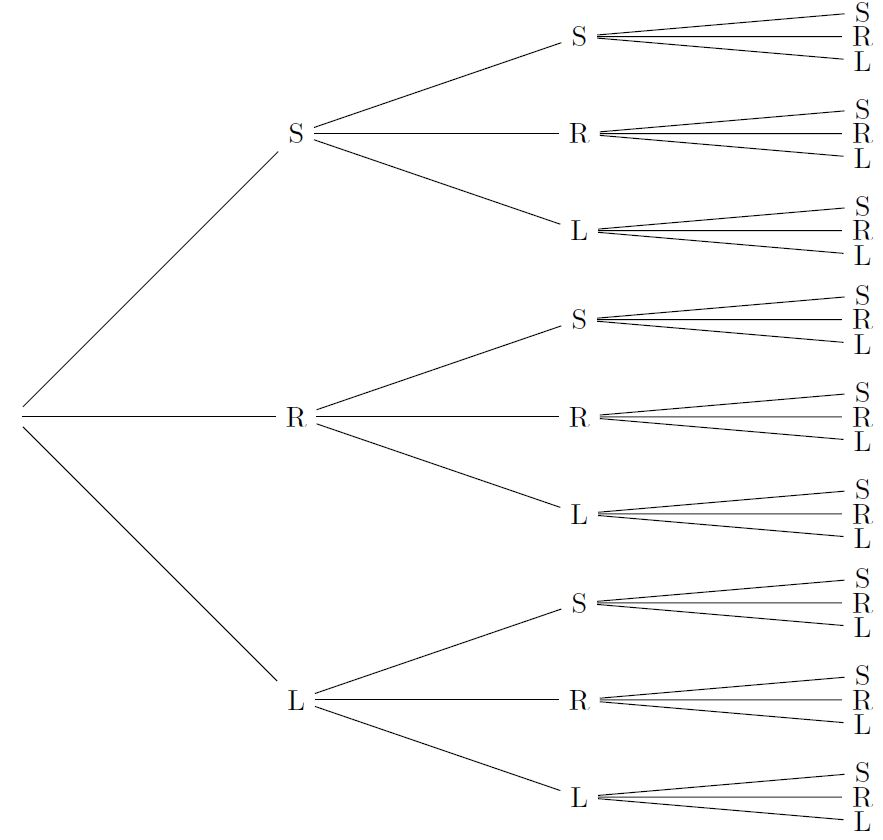
\includegraphics[width=12.26in]{./figures/vehicles} 

}

\caption{A tree diagram representing the choices for the three vehicles}\label{fig:tree}
\end{figure}

\begin{enumerate}
\def\labelenumi{\alph{enumi})}
\item
  \(0.35^3\)
\item
  \(0.45^3+0.2^3+0.35^3\)
\item
  LLR can be rearranged in \(3\) ways: LLR, LRL, RLL. \(3\times 0.45^2 \times 0.2\).
\item
  SRL can be rearranged in \(3!\) ways. \(3!\times 0.35 \times 0.45 \times 0.2\).
\item
  LLR or LLS. Each can be rearranged in \(3\) ways, then these are mutually exclusive outcomes so we can add the probabilities. \[3\times 0.45^2 \times 0.2 + 3\times 0.45^2 \times 0.35\].
\end{enumerate}

\hypertarget{conditional-probability}{%
\section{Conditional Probability}\label{conditional-probability}}

We will consider the following examples to motivate the definition of conditional probability.

\begin{example}

The number of insurance claims in the previous \(12\) months is cross tabulated with whether the driver involved was a young driver.

\begin{longtable}[]{@{}crrr@{}}
\toprule
& Under 25 & 25 and over & Total\tabularnewline
\midrule
\endhead
No claim & 225 & 725 & 950\tabularnewline
Claim & 25 & 25 & 50\tabularnewline
& 250 & 750 & 1000\tabularnewline
\bottomrule
\end{longtable}

\end{example}

The insurance company is interested in the claim rate. Overall the claim rate is,

\[\text{P}(\text{Claim})=\frac{50}{1000} = 0.05\]

An estimate for the probability of a driver claiming on the insurance is then \(1\) in \(20\).

However this figure hides a substantial difference in the claim rates for young and older drivers.

If we consider the \(250\) young drivers separately we have,

\[\text{P}(\text{Claim}|\text{Under}\ 25)=\frac{25}{250} = 0.1.\]
Whereas for the \(750\) older drivers we have,

\[\text{P}(\text{Claim}| 25 \ \text{and over})=\frac{25}{750} = 0.03.\]

The notation \(|\) is read `given that' and is a conditional statement. The conditional probabilities show that the claim rate is much higher for the younger drivers. One can compute the ratio of these probabilities to see how many times higher it is, \(0.1/0.03 \approx 3.3\), so this is just over three times higher. This relative risk scoring is common in medical statistics.

\begin{example}
\protect\hypertarget{exm:cancer}{}\label{exm:cancer}Consider the following data from a study on male lung cancer patients carried out in \(1950\) in the UK. This was one of the earliest applications of epidemiology - the use of statistics to study disease patterns in populations.

\begin{longtable}[]{@{}crrr@{}}
\toprule
& Non-smoker & Smoker & Total\tabularnewline
\midrule
\endhead
Lung cancer & 2 & 647 & 649\tabularnewline
No lung cancer & 27 & 620 & 647\tabularnewline
& 29 & 1267 & 1296\tabularnewline
\bottomrule
\end{longtable}

Calculate the relative risk of having lung cancer for a smoker compared to a non-smoker.

\emph{solution}

\[\text{P}(\text{Lung cancer}|\text{Smoker}) = \frac{647}{1267}\]

\[\text{P}(\text{Lung cancer}|\text{Non-smoker}) = \frac{2}{29}\]

There is \(\approx 7.4\) times higher relative risk of lung cancer in smokers.
\end{example}

These examples motivate the definition of conditional probability.

\begin{definition}[conditional probability]
The \textbf{\emph{conditional probability}} \(\text{P}(A|B)\) of an event \(A\) given another event of non-zero probability \(B\) is given by,

\[\text{P}(A|B) = \frac{\text{P}(A\cap B)}{\text{P}(B)}.\]
\end{definition}

One should verify that the fraction on the left is precisely how the conditional probability was calculated in the previous two examples.

\begin{theorem}
The conditional probability \(\text{P}(A|B)\) satisfies Kolmogorov's definition of probability.
\end{theorem}

\begin{proof}
Not lectured or examined, but here for completeness.

Firstly need to check \(P(A|B)\in[0,1]\). We have \(P(A|B) \geq 0\) because \(P(A\cap B)\geq0\) and \(P(B)>0\).

Because the intersection of \(B\) with another set is contained in \(B\), we have \(A\cap B \subseteq B\), and so
\[P(A\cap B) \leq P(B).\]
And dividing through by \(P(B)\) gives \(P(A|B) \leq 1\).

Secondly, \[P(\Omega|B) = \frac{P(\Omega \cap B)}{P(B)} = \frac{P(B)}{P(B)}=1.\]

Lastly, any given any two disjoint \(A_1\),\(A_2\) such that \(A_1\cap A_2 = \varnothing\).

We have that

\begin{align}
P(A_1\cup A_2 |B) &= \frac{P((A_1\cup A_2)\cap B)}{P(B)} \\
&= \frac{P((A_1\cap B)\cup (A_2\cap B))}{P(B)} \\
&= \frac{P(A_1\cap B)}{P(B)} + \frac{P(A_2\cap B)}{P(B)} \\
&= P(A_1|B) + P(A_2|B)
\end{align}
\end{proof}

\begin{example}
Note that \(P(A|B) \neq P(B|A)\). Revisiting the driver's example gives,

\begin{longtable}[]{@{}crrr@{}}
\toprule
& Under 25 & 25 and over & Total\tabularnewline
\midrule
\endhead
No claim & 225 & 725 & 950\tabularnewline
Claim & 25 & 25 & 50\tabularnewline
& 250 & 750 & 1000\tabularnewline
\bottomrule
\end{longtable}

\[\text{P}(\text{Claim}|\text{Under}\ 25)=0.1.\]
However,
\[\text{P}(\text{Under}\ 25|\text{Claim})=\frac{25}{50} = 0.5\]
\end{example}

\begin{theorem}
Two events \(A\) and \(B\) are \emph{independent} if and only if
\[\text{P}(A|B) = \text{P}(A) \ \text{ or } \ \text{P}(B|A) = \text{P}(B)\]
In other words, conditioning on either event does not affect the probability of the other event occurring.
\end{theorem}

\begin{proof}
Using the definition of conditional probability,
\[\text{P}(A\cap B) = \text{P}(A|B)\text{P}(B)=\text{P}(B|A)\text{P}(A)\]
If
\[\text{P}(A|B) = \text{P}(A) \ \text{ or } \ \text{P}(B|A) = \text{P}(B),\]
substituting this in the former yields
\[\text{P}(A\cap B) = \text{P}(A)\text{P}(B), \]
which is the definition of independence.
Conversely if two events are independent, we have
\[\text{P}(A|B) = \frac{\text{P}(A\cap B)}{\text{P}(B)} = \frac{\text{P}(A)\text{P}(B)}{\text{P}(B)} = \text{P}(A), \]
and likewise for \(\text{P}(B|A)\).
\end{proof}

When constructing tree diagrams the probabilities involved are usually conditional probabilities as there is a natural progression through the tree from left to right conditioning on what happened previously. In the diagram below, the events \(A\) and \(B\) may not be independent.

\begin{figure}

{\centering 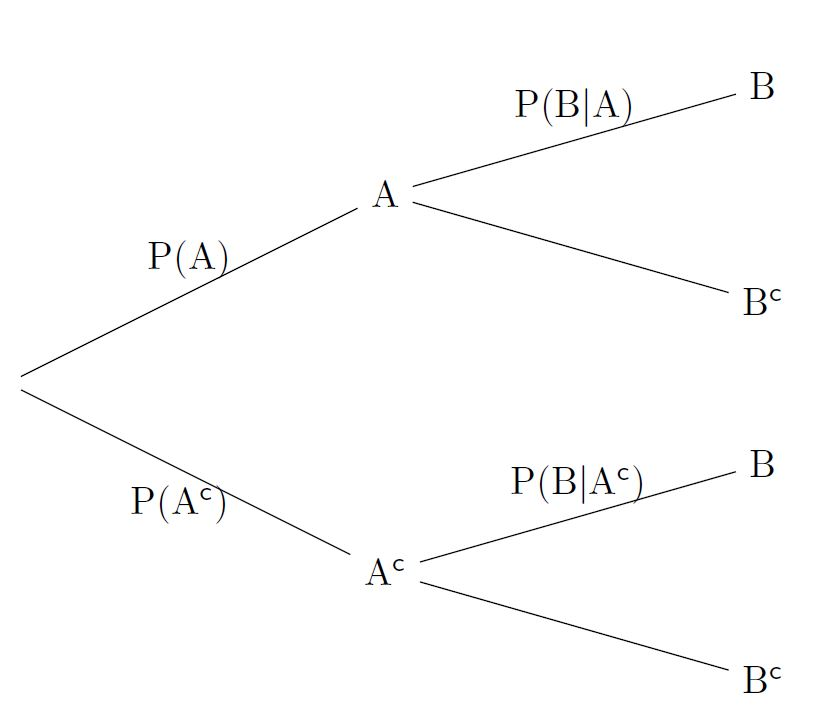
\includegraphics[width=11.31in]{./figures/condtree} 

}

\caption{The second level of branches represent the conditional probabilities of B given A or its complement, which may be different numbers}\label{fig:tree2}
\end{figure}

\begin{example}
Jon always goes to campus by bike or takes a tram. If one day he goes to campus by bike, the probability that he goes to campus by tram the next day is \(0.4\). If one day he goes to campus by tram, the probability that he goes to campus by bike the next day is \(0.7\).
Given that Jon goes to campus on Monday by tram, find the probability that he takes a tram to campus on Wednesday.

\emph{solution}

This may be solved by considering a tree diagram with levels for Tuesday and Wednesday. The probabilities in the question are \(\text{P}(\text{tram} \ |\ \text{bike})=0.4\) and \(\text{P}(\text{bike} \ |\ \text{tram})=0.7\).
Monday's journey is done. Possible sequences are `tram then tram', or `bike then tram'. These are mutually exclusive outcomes. The calculation is then

\[0.3^2+0.7\times 0.4 = 0.37\].
\end{example}

Surveys with questions of a sensitive or delicate nature often result in respondents missing that question or lying about their answers. Conditional probability can be used to mask the awkward question and find the proportion who would answer a certain way.

\begin{example}
A company want to find the proportion of employees who have ever called in sick to work, when in fact they were not sick. The boss asks each employee to toss a coin and hide the result.

If the result is \textbf{\emph{heads}}, the employee should answer the question `is your age an odd number?'.

If the result is \textbf{\emph{tails}}, they should answer `Have you ever taken a day off when you should not have?'.

Because the boss does not know which question people are answering, the employees can answer truthfully.

Suppose that \(40\%\) of employees mark `yes' as their answer. Let,

\[p= \text{P}(\text{taken a day off} \ | \ \text{tails})\]
Assume that ages are randomly distributed so that the chance of an even or odd number of years old is \(0.5\). How can we find \(p\)?
\end{example}

\emph{solution}

One can draw a tree diagram.

\begin{figure}

{\centering 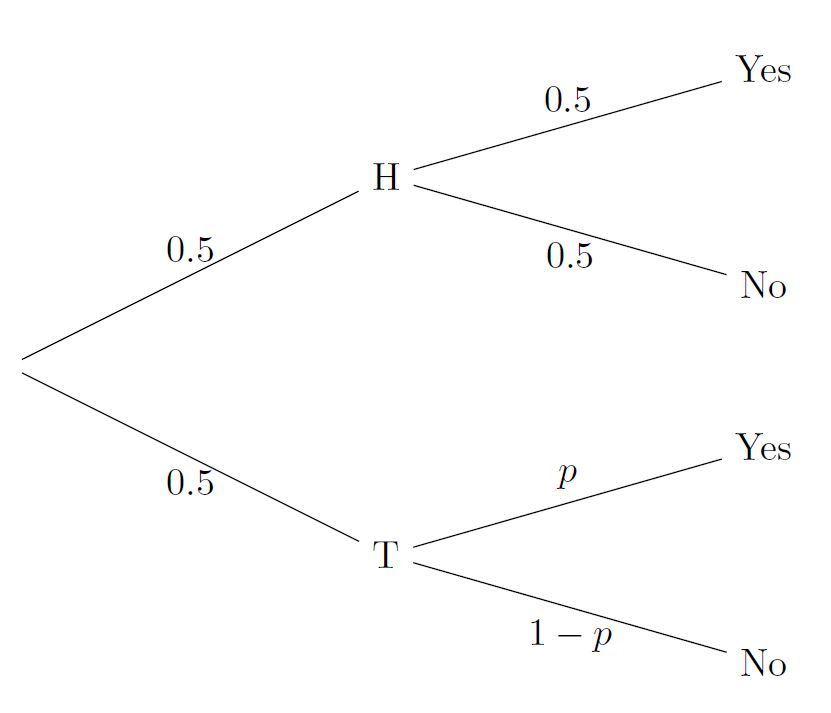
\includegraphics[width=11.54in]{./figures/survey} 

}

\caption{The outcomes of the survey.}\label{fig:tree3}
\end{figure}

The overall probability of answering `yes' is \(0.25+0.5p\), and in the survey \(40\%\) answered `yes'. We then have

\[0.25+0.5p = 0.4, \]
and hence \(p=0.3\). This means we can estimate that \(30\%\) of employees have taken a day of when they were not supposed to.

\hypertarget{bayes-theorem}{%
\section{Bayes Theorem}\label{bayes-theorem}}

\begin{example}
There are two coins in a bag. One coin is fair, while the other has heads on both sides (a double-header).

A coin is selected from the bag at random, and the selected coin is flipped three times. Unfortunately the coin which was selected is unknown to us.

On each of three flips the coin comes up heads.

Without doing any calculations, how likely do you think it is to be the unfair coin?
\end{example}

\emph{solution}

Let
\(A =\left\{ \text{The double-header is selected} \right\}\) and
\(B =\left\{ \text{The coin lands heads up three times in a row} \right\}\)

\begin{figure}

{\centering 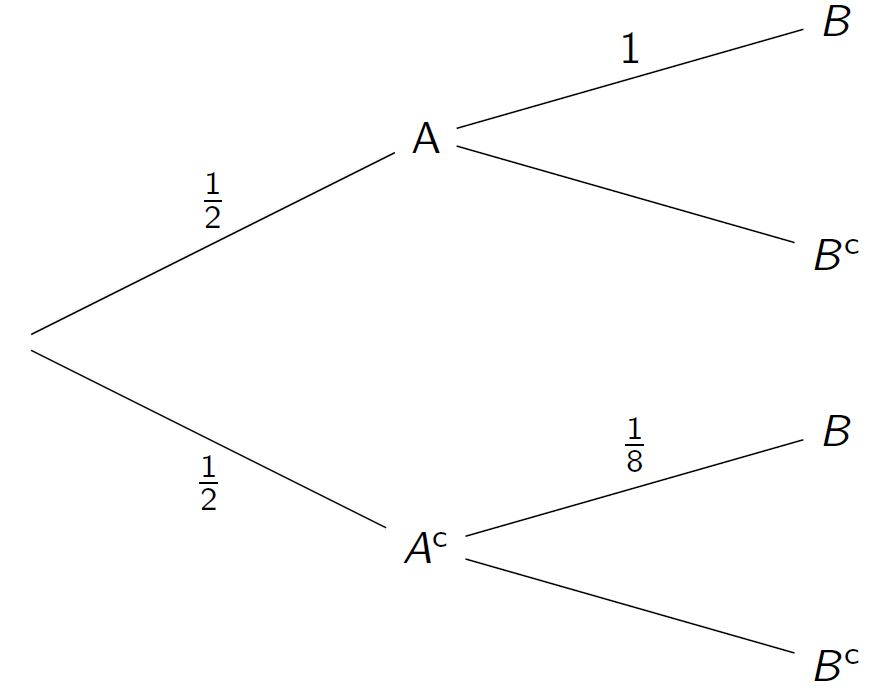
\includegraphics[width=12.38in]{./figures/doubleheader} 

}

\caption{A tree diagram for the double headed coin example.}\label{fig:tree4}
\end{figure}

One can use the tree diagram to find \(8/9\).

We can generalise this picture and come up with a formula for the conditional probability called Bayes' formula.

\begin{figure}

{\centering 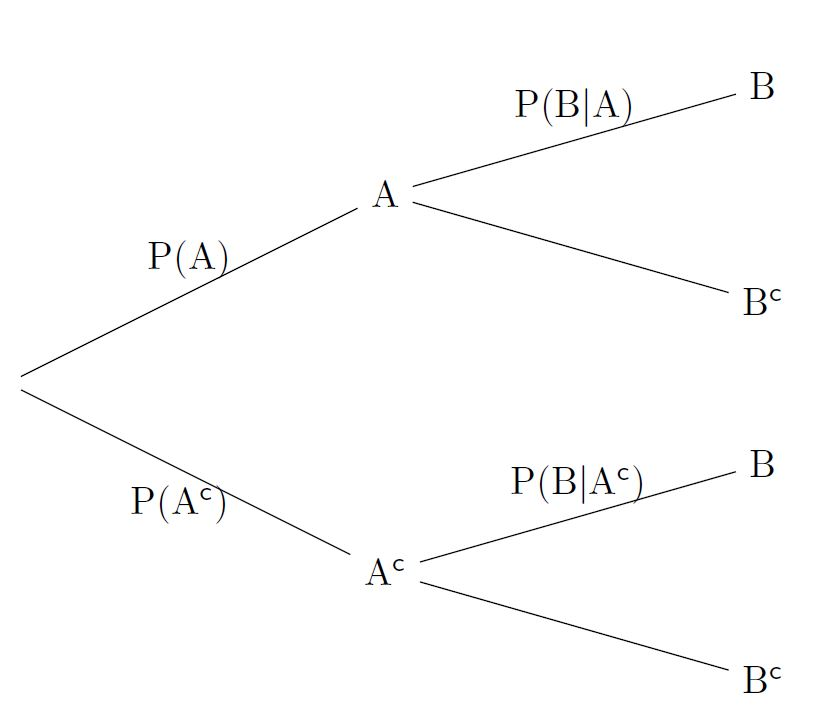
\includegraphics[width=11.31in]{./figures/condtree} 

}

\caption{Tree showing Bayes' formula}\label{fig:tree5}
\end{figure}

\[P(A|B) = \frac{P(A\cap B)}{P(B)} = \frac{P(A)P(B|A)}{P(A)P(B|A)+P(A^{\mathsf{c}})P(B|A^{\mathsf{c}})}\]

Previously, \(A_1=A\) and \(A_2 = A^{\mathsf{c}}\) are disjoint and their union gives the entire sample space. This situation is called a \emph{partition}.

This can be extended to a partition of \(n\) events \(A_1,A_2, \dots , A_n\).

\begin{definition}
A collection of events \(A_1, A_2, \dots , A_n\) is a \textbf{\emph{partition}} if their union is the entire sample space, that is \emph{exhaustive}, and they are mutually exclusive. That is

\begin{enumerate}
\def\labelenumi{\roman{enumi})}
\item
  \(\Omega = A_1 \cup A_2 \cup \dots \cup A_n\).
\item
  \(A_1 \cap A_2 \cap \dots \cap A_n = \varnothing\)
\end{enumerate}

Any event and its complement form a partition.
\end{definition}

Here is a picture of a partition:

\begin{figure}

{\centering 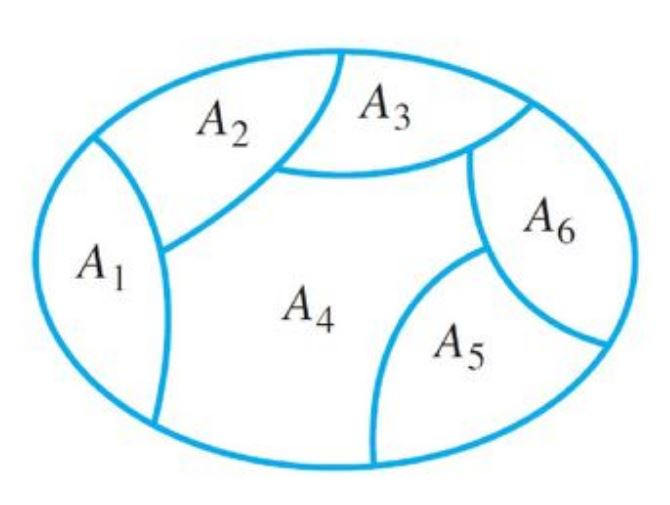
\includegraphics[width=9.31in]{./figures/partition} 

}

\caption{An example partition with six sets.}\label{fig:partition}
\end{figure}

We can now extend the concept of conditional probability to a general situation in which we condition on the event of at least one event of a partition.

\begin{theorem}[Law of Total Probability]
Suppose we have a partition \(A_1, A_2, \dots , A_n\) of the sample space \(\Omega\). Then for any event \(B \subseteq \Omega\), we have

\[\text{P}(B) =P(A_1)P(B|A_1)+ \dots + P(A_n)P(B|A_n) \]
\end{theorem}

An intuitive proof is to imagine a tree diagram with \(n\) branches for each of the \(A_i\) in the first layer, then \(B\) and \(B^{\mathsf{c}}\) in the next layer. As you multiply along all the branches the ways that \(B\) can occur you end up with the sum in the RHS.

\begin{theorem}[Bayes' Theorem]
Suppose we have a partition \(A_1, A_2, \dots , A_n\) of the sample space \(\Omega\). Then the conditional probability of any one event of the partition \(A_k\) for some \(k\), given any other event \(B\) can be written as,

\[\text{P}(A_k |B) = \frac{\text{P}(B|A_k)\text{P}(A_k)}{\sum^{n}_{i=1}\text{P}(B|A_i)P(A_i)}\]
\end{theorem}

\begin{proof}
Note that \(\text{P}(A_k\cap B) = \text{P}(B|A_k)\text{P}(A_k)\),

and that the denominator is \$\text{P}(B) using the law of total probability.
\end{proof}

\begin{example}
A company produces electrical components using three shifts. During the first shift \(50%
\) of components are produced, with \(20\%\) and \(30\%\) being produced during shifts \(2\) and \(3\) respectively. The proportion of defective components produced during shift \(1\) is \(6\%\). For shifts \(2\) and \(3\) the proportions are \(8\%\) and \(12\%\) respectively.

\begin{enumerate}
\def\labelenumi{\alph{enumi})}
\item
  Find the percentage of defective components.
\item
  If a component is defective, what is the probability that it came from shift \(3\)?
\end{enumerate}

\emph{solution}

Let \(D\) be the event that the component is defective and \(S_1,S_2,S_3\) denotethat it was produced during shifts \(1,2\) or \(3\) respectively.

\begin{enumerate}
\def\labelenumi{\alph{enumi})}
\item
  Use the theorem of total probability, as follows:
  \begin{align}
  \text{P}(D)  &= \text{P}(D|S_1)P(S_1)+\text{P}(D|S_2)\text{P}(S_2)+\text{P}(D|S_3)\text{P}(S_3) \\
  &= 0.06\times 0.5 + 0.08\times 0.2 + 0.12\times 0.3 \\
  &= 0.082
  \end{align}
\item
  Using Bayes' theorem,
\end{enumerate}

\[\text{P}(S_3|D) = \frac{\text{P}(D|S_3)\text{P}(S_3)}{\text{P}(D)}\]
The denominator was worked out in part a), this gives \(\frac{0.12\times 0.3}{0.082}=0.439\).
\end{example}

Bayes' theorem allows us to update the probability of an event in the light of new evidence. This is in fact the main practical use of the theorem, and leads to a whole branch of Bayesian Statistics.

\begin{example}
Gary is suspected of committing a crime. The evidence so far points to a probability of guilt being \(0.9\). To `prove his innocence' Gary undergoes a lie detector test, which has a \(70\%\) accuracy rate. The test will say positive to indicate guilt, and negative to indicate not guilty. The test is such that
\[\text{P}(\text{Positive}|\text{Guilty}) = 0.7\]
\[\text{P}(\text{Negative}|\text{Innocent})=0.7\]

If Gary's test comes back \textbf{\emph{negative}}, what is then the probability of his guilt?

\emph{solution}

One can directly apply Bayes' theorem.
\[\text{P}(\text{Guilt}|\text{Negative})=\frac{\text{P}(\text{Negative}|\text{Guilt})\text{P}(\text{Guilt})}{\text{P}(\text{Negative}|\text{Guilt})\text{P}(\text{Guilt})+\text{P}(\text{Negative}|\text{Innocent})\text{P}(\text{Innocent})}\]
and so
\[\text{P}(\text{Guilt}|\text{Negative})=\frac{0.3\times 0.9}{0.3\times 0.9 \ + \ 0.7\times 0.1}=0.794 \ \text{(3 d.p.)}\]
\end{example}

Beware of having extreme prior beliefs, for no evidence can then change your mind. Believing something to be true \(100\%\) or \(0\%\), will mean that no reason or evidence will change this position.

\begin{example}[Cromwell's Rule]
If we believe Gary is \(100\%\) guilty at the start then
\[\text{P}(\text{Guilt}|\text{Negative})=\frac{0.3\times 1}{0.3\times 1 \ + \ 0.7\times 0}=1\]
So we would still believe Gary to be \(100\%\) guilty.

If we believe Gary is \(0\%\) guilty at the start then
\[\text{P}(\text{Guilt}|\text{Negative})=\frac{0.3\times 0}{0.3\times 0 \ + \ 0.7\times 1}=0\]
So we would still believe Gary to be \(0\%\) guilty.
\end{example}

As educated people we should always consider the opposing opinion and update our own beliefs according to the evidence available. If you have a strong opinion about something, consider what would change your mind. Always leave some room to doubt yourself, because you could be wrong.

\hypertarget{exercises-week-2}{%
\section{Exercises Week 2}\label{exercises-week-2}}

\begin{exercise}

I toss a fair coin and roll a die.
a) Are these events independent?

\begin{enumerate}
\def\labelenumi{\alph{enumi})}
\setcounter{enumi}{1}
\tightlist
\item
  What is the probability I obtain a head and a \(6\)?
\end{enumerate}

\end{exercise}

\begin{exercise}

A torch uses two batteries in series. Each battery works with probability \(0.95\), independently of the other. Work out the probability that:

\begin{enumerate}
\def\labelenumi{\alph{enumi})}
\item
  The torch will work.
\item
  Both batteries fail
\item
  Only one of the batteries will work.
\end{enumerate}

\end{exercise}

\begin{exercise}
Whether a student gets up on time depends on whether or not he has remembered to set his alarm the night before. Some \(90\%\) of the time he remembers, the other \(10\%\) he forgets. When the clock is set, he will get up on time \(95\%\) of occasions. If it is not set, the chance he will oversleep is \(35\%\). Use a tree diagram to find the probability that he will oversleep.
\end{exercise}

\begin{exercise}
The following data shows the distribution of male and female students on various degree courses at a university.

\begin{longtable}[]{@{}cccc@{}}
\toprule
& Accountancy & Economics & Finance\tabularnewline
\midrule
\endhead
Male & 330 & 360 & 90\tabularnewline
Female & 120 & 390 & 60\tabularnewline
\bottomrule
\end{longtable}

Suppose a student is selected at random. Find the probability that they are,

\begin{enumerate}
\def\labelenumi{\alph{enumi})}
\item
  female
\item
  studying Economics
\item
  male and studying Economics
\item
  male given that they are studying Economics
\item
  female given that they are studying Economics
\item
  studying Economics given that they are female
\end{enumerate}

Are the events `student is male' and `studying Economics' independent?
\end{exercise}

\begin{exercise}

The following table shows the lung cancer data for females in the same \(1950\) study given in example \ref{exm:cancer}.

\begin{longtable}[]{@{}crrr@{}}
\toprule
& Non-smoker & Smoker & Total\tabularnewline
\midrule
\endhead
Lung cancer & 19 & 41 & 60\tabularnewline
No lung cancer & 32 & 28 & 60\tabularnewline
& 51 & 69 & 120\tabularnewline
\bottomrule
\end{longtable}

\begin{enumerate}
\def\labelenumi{\alph{enumi})}
\item
  Calculate the relative risk for female smokers compared to non-smokers.
\item
  Can you suggest any reason for the difference in the figures between males and females?
\end{enumerate}

\end{exercise}

\begin{exercise}

Two electrical components \(X\) and \(Y\) have probabilities of working \(\frac{3}{4}\) and \(\frac{7}{8}\), respectively. They also function independently of each other. Two devices \(D_1\) and \(D_2\) are constructed. In \(D_1\), \(X\) and \(Y\) are in series, and in \(D_2\) they are wired in parallel.

\begin{enumerate}
\def\labelenumi{\alph{enumi})}
\item
  \begin{enumerate}
  \def\labelenumii{(\roman{enumii})}
  \tightlist
  \item
    Find the probability that \(D_1\) works.
  \end{enumerate}
\end{enumerate}

\begin{enumerate}
\def\labelenumi{(\roman{enumi})}
\setcounter{enumi}{1}
\tightlist
\item
  Find the probability that \(D_2\) works.
\end{enumerate}

\begin{enumerate}
\def\labelenumi{\alph{enumi})}
\setcounter{enumi}{1}
\tightlist
\item
  Suppose that \(D_1\) works, find the probability that;
\end{enumerate}

\begin{enumerate}
\def\labelenumi{(\roman{enumi})}
\tightlist
\item
  \(X\) is working.
\item
  Only \(X\) is working.
\item
  both \(X\) and \(Y\) are working.
\end{enumerate}

\begin{enumerate}
\def\labelenumi{\alph{enumi})}
\setcounter{enumi}{2}
\tightlist
\item
  Suppose that \(D_2\) works, find the probability that;
\end{enumerate}

\begin{enumerate}
\def\labelenumi{(\roman{enumi})}
\tightlist
\item
  \(X\) is working.
\item
  Only \(X\) is working.
\item
  both \(X\) and \(Y\) are working.
\end{enumerate}

\end{exercise}

\begin{exercise}

An urn contains two green balls and three red bals. Supose two balls will be drawn at random one after another and without replacement. Draw a tree diagram, and find the probability that:

\begin{enumerate}
\def\labelenumi{\alph{enumi})}
\item
  a green ball appears on the first draw.
\item
  a green ball appears in the second draw.
\end{enumerate}

\end{exercise}

\begin{exercise}
The following table shows the \emph{fear factor} for children attending the dentist, cross tabulated with the School age of the child.

\begin{longtable}[]{@{}lccc@{}}
\toprule
& Infant & Primary & Secondary\tabularnewline
\midrule
\endhead
Afraid & 0.12 & 0.08 & 0.05\tabularnewline
Not afraid & 0.28 & 0.25 & 0.22\tabularnewline
\bottomrule
\end{longtable}

For a child selected at random define the events; \(A = \{ \text{The child is afraid} \}\),

with \(N\) being not afraid, and \(I\),\(P\) and \(S\) being the School age in the obvious fashion.

Calculate the following probabilities,

\begin{enumerate}
\def\labelenumi{\alph{enumi})}
\item
  \(\text{P}(A)\), \(\text{P}(N)\), \(\text{P}(A\cup I)\).
\item
  \(\text{P}(A| I)\) and \(\text{P}(I| A)\).
\item
  \(\text{P}(A| S)\) and \(\text{P}(N| S)\) - what do you notice about these two probabilities?
\end{enumerate}

Are \(A\) and \(I\) independent?
\end{exercise}

\begin{exercise}
A survey by an electrical retailer determines that \(40\%\) of customers who seek advice from sales staff by an appliance and only \(20\%\) who do not seek advice buy an appliance. If \(30\%\) of customers seek advice, what is the probability that a customer entering the warehouse buys an appliance?
\end{exercise}

\begin{exercise}

Four cards are drawn at random without replacement from a deck of \(52\) cards. What is the probability that the sequence is:

\begin{enumerate}
\def\labelenumi{\alph{enumi})}
\item
  \(\heartsuit\) \(\heartsuit\) \(\spadesuit\) \(\clubsuit\)
\item
  \(\heartsuit\) \(\heartsuit\) \(\spadesuit\) \(\spadesuit\)
\end{enumerate}

\end{exercise}

\begin{exercise}

A student comes back from a night at the pub with a bunch of keys, only one of which works. They try one key at random in the lock and discard it if it doesn't fit.

\begin{enumerate}
\def\labelenumi{\alph{enumi})}
\tightlist
\item
  Suppose the bunch contains \(2\) keys. Find the probability they open the door on
\end{enumerate}

\begin{enumerate}
\def\labelenumi{(\roman{enumi})}
\item
  the first attempt
\item
  the second attempt
\end{enumerate}

\begin{enumerate}
\def\labelenumi{\alph{enumi})}
\setcounter{enumi}{1}
\item
  Repeat for a bunch of three keys being successul at the first, second and third attempts.
\item
  Suppose now that the bunch contains \(n\) keys. Find the probability that the door is opened on the \(r^{\text{th}}\) attempt (where \(1\leq r \leq n\)).
\end{enumerate}

\end{exercise}

\begin{exercise}
To ascertain the proportion of people who have had a sexually transmitted infection, the following survey pocedure was used on \(1000\) individuals.

They were asked to think of the day of the week their most recent birthday fell on.

If their last birthday was on a Monday, Tuesday or Wednesday they were to answer the question `Have you every had a sexually transmitted infection?'.

If their last birthday was on any other day of the week, they were to answer the question `Is your age an even number?'.

In the survey \(290\) people answered `yes'. Assuming that ages and birthdays are uniformly distributed, can you estimate the proportion of people who have had a sexually transmitted infection?
\end{exercise}

\begin{exercise}
Suppose two events \(A\) and \(B\) are independent. Show that \(A\) and \(B^{\mathsf{c}}\) are also independent. Show also that \(A^{\mathsf{c}}\) and \(B^{\mathsf{c}}\) are independent.
\end{exercise}

\begin{exercise}

Forty percent of new employees hired by a large company have a degree. Seventy percent of employees with degrees are promoted within two years.Of those without degrees, only \(30\%\) arepromoted within two years.

\begin{enumerate}
\def\labelenumi{\alph{enumi})}
\item
  What is the probability that a new empoyee will be promoted?
\item
  If an employee has been promoted, what is the probability that they have a degree?
\end{enumerate}

\end{exercise}

\begin{exercise}
A bag contains \(3\) coins; two are normal unbiased coins while the third is double headed. A coin is chosen at random from the bag and tossed. The coin is tossed \(4\) times and came up heads each time. What is the probability that it is the double header?
\end{exercise}

\begin{exercise}
Approximately \(25\%\) of males over \(50\) have some form of heart problem. A clinic has observed that males with a heart problem are three times more likely to be smokers as males with no heart problem. What is the probability that a male over \(50\) has a heart problem given that he is a smoker?
\end{exercise}

\begin{exercise}

Cage A contains five hens with disease and six hens without disease. Cage B contains two diseased hens and five hens without the disease. Two hens are chosen at random from cage A and transferred to cage B. A hen is now chosen at random from cage B and found to be diseased. Find the probability that the two hens that were transferred were,

\begin{enumerate}
\def\labelenumi{\alph{enumi})}
\item
  both diseased
\item
  both without disease.
\end{enumerate}

\end{exercise}

\hypertarget{drv}{%
\chapter{Discrete Random Variables}\label{drv}}

In most practical situations in which we encounter uncertainty, the random outcome of interest is a numerical quantity. This could be the number of minutes you end up waiting for that bus, how much you win on the lottery this week, or even the number of times you try to catch a fly with chopsticks before you eventually manage to do so.

\hypertarget{random-variables}{%
\section{Random Variables}\label{random-variables}}

In this chapter you will learn the concept of a discrete random variable.

\begin{example}
Suppose we roll two dice and find the sum of the numbers on the two dice. Let \(X\) be the sum of the numbers on the two dice. We know the sample space here is:
\[\Omega = \{ (n_1,n_2) : n_1,n_2 \in \mathbb{N}, \ 1 \leq n_1 , n_2 \leq 6 \},\]
Given an outcome \((n_1,n_2)\), the `variable' \(X\) takes a particular whole numbered value from \(x=2, \dots , 12\). We have seen that these particular values are not equally likely.
\end{example}

\begin{definition}
A \textbf{\emph{random variable}} \(X\) is a set function which maps the potential outcomes of a statistical experiment to (some subset of) the real number line.

A random variable is written with a capital letter (here \(X\)), and the particular values it takes are written with a lowercase of the same letter (here \(x\)). The probability that \(X\) takes a particular value is written \(\text{P}(X=x)\).
\end{definition}

Just as with data analysis there is a difference between \emph{discrete} and \emph{continuous} random variables. One can think of \emph{discrete} random variables arising from a process which involves counting and can take integer values. The \emph{continuous} random variables can be thought of as arising from a measuring process.

\begin{example}
Let \$R = \$ result of spinning a roulette wheel. The roulette wheel can take particular values
\[\Omega = \{0,1,2, \dots,36\}.\]
In number ranges from 1 to 10 and 19 to 28, odd numbers are red and even are black. In ranges from 11 to 18 and 29 to 36, odd numbers are black and even are red. There is a green pocket numbered 0 (zero). Then \(R\) is a discrete random variable, as it takes only particular discrete values.

Let \(T =\) the time spent waiting for a bus. Here \(T\) could be any positive number from when you arrive at the bus stop (if it were time after the timetabled arrival time, it could be negative for an early bus). Then \(T\) is a continuous random variable.
\end{example}

We will consider discrete random variables first, but will study both types in this course.

\hypertarget{discrete-probability-distributions}{%
\section{Discrete probability distributions}\label{discrete-probability-distributions}}

In order to understand how a random variable is likely to behave, and thus be able to predict its possible future values, we clearly need to consider the probability with which it will take on particular values. This set of probability values is known as a probability distribution. We will develop the theory with some examples.

\begin{definition}
The \textbf{\emph{distribution}} function, also known as a \textbf{\emph{probability mass function}}, of a random variable \(X\) is the function that outputs the probability of \(X\) attaining any particular value. That is,

\[f(x) = \text{P}(X=x)\]
In some texts, or if there are two variables in play, we may also write the variable in subscript \(f_X(x)\) to be clear to which mass function we are referring.
\end{definition}

\begin{example}[discrete uniform distribution]

Consider rolling a fair die and let the discrete random variable \(X\) be the score observed on the die. We know that the probability of getting any of the particular values in the set \(\{1,2, \dots 6\}\) is \(\frac{1}{6}\) and this is the probability distribution. We may tabulate the values as follows

\begin{longtable}[]{@{}cllllll@{}}
\toprule
\begin{minipage}[b]{0.28\columnwidth}\centering
\(x\)\strut
\end{minipage} & \begin{minipage}[b]{0.09\columnwidth}\raggedright
1\strut
\end{minipage} & \begin{minipage}[b]{0.09\columnwidth}\raggedright
2\strut
\end{minipage} & \begin{minipage}[b]{0.09\columnwidth}\raggedright
3\strut
\end{minipage} & \begin{minipage}[b]{0.09\columnwidth}\raggedright
4\strut
\end{minipage} & \begin{minipage}[b]{0.09\columnwidth}\raggedright
5\strut
\end{minipage} & \begin{minipage}[b]{0.09\columnwidth}\raggedright
6\strut
\end{minipage}\tabularnewline
\midrule
\endhead
\begin{minipage}[t]{0.28\columnwidth}\centering
\(\text{P}(X=x)\)\strut
\end{minipage} & \begin{minipage}[t]{0.09\columnwidth}\raggedright
\(\frac{1}{6}\)\strut
\end{minipage} & \begin{minipage}[t]{0.09\columnwidth}\raggedright
\(\frac{1}{6}\)\strut
\end{minipage} & \begin{minipage}[t]{0.09\columnwidth}\raggedright
\(\frac{1}{6}\)\strut
\end{minipage} & \begin{minipage}[t]{0.09\columnwidth}\raggedright
\(\frac{1}{6}\)\strut
\end{minipage} & \begin{minipage}[t]{0.09\columnwidth}\raggedright
\(\frac{1}{6}\)\strut
\end{minipage} & \begin{minipage}[t]{0.09\columnwidth}\raggedright
\(\frac{1}{6}\)\strut
\end{minipage}\tabularnewline
\bottomrule
\end{longtable}

\end{example}

Alternatively we may use a formula:
\begin{equation*}
  f(x)=\begin{cases}
    \frac{1}{6}, & \text{if } x = 1, 2, \dots , 6.\\
    0 & \text{otherwise}.
  \end{cases}
\end{equation*}

Or a graph:

\begin{figure}

{\centering 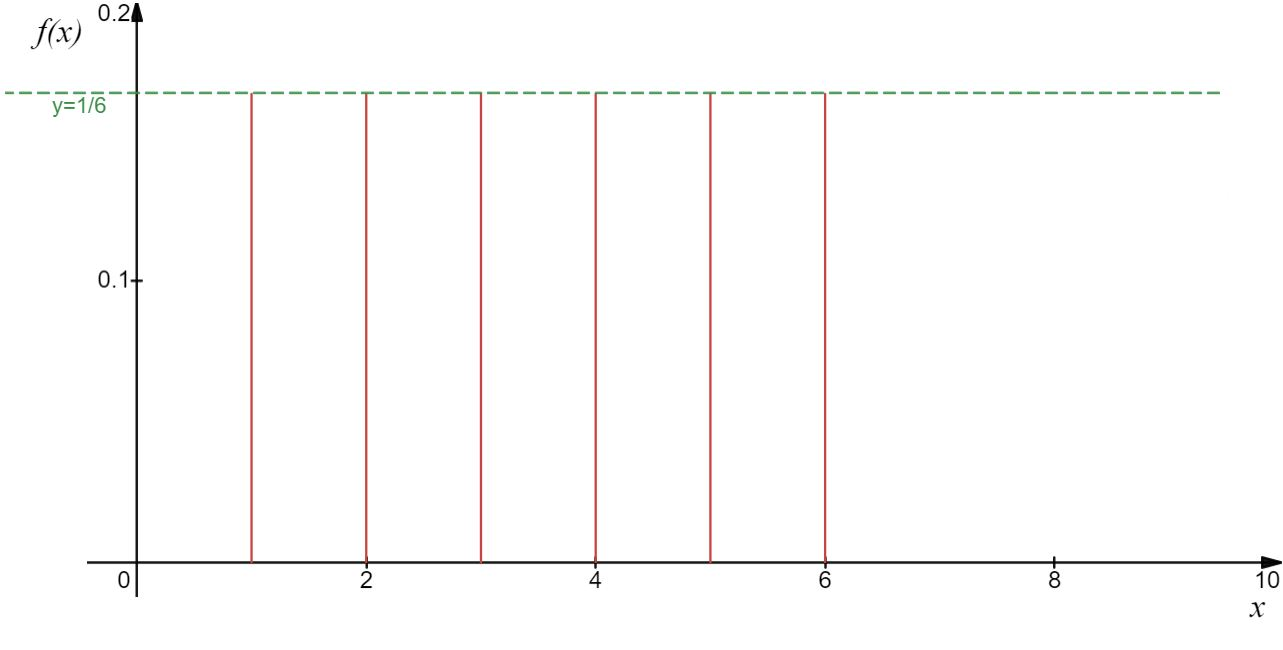
\includegraphics[width=0.75\linewidth]{./figures/uni_pdf} 

}

\caption{Probability mass function for a fair die}\label{fig:uniformdice}
\end{figure}

Clearly the graph is a very useful way to visualise how the probability is distributed. You can also see why this is called a discrete \emph{uniform} distribution - it's because the values are all the same.

Some questions to consider:

\begin{itemize}
\item
  Suppose your die had \(n\) sides, where \(n\) is some whole number greater than \(1\), and the faces numbered \(1,2,\dots n\). What does the distribution look like now?
\item
  Can you represent the distribution in each of the three ways above?
\end{itemize}

\begin{example}[Urn problem]
An urn contains five balls numbered \(1\) to \(5\). Two balls are drawn simultaneously.

\begin{enumerate}
\def\labelenumi{\arabic{enumi}.}
\item
  Let \(X\) be the larger of the two numbers.
\item
  Let \(Y\) be the sum of the two numbers.
\end{enumerate}

Find the probability distributions of \(X\) and \(Y\).

\emph{solution}

\begin{enumerate}
\def\labelenumi{\arabic{enumi}.}
\tightlist
\item
  We proceed as follows by enumerating all the possibilities and noting that there are \(^5C_2=10\) ways of drawing the balls from the urn. Note here that as the balls are drawn simultaneously, order does not matter here.
\end{enumerate}

To find the distribution of \(X\) one can list the outcomes systematically by the largest value.

\begin{longtable}[]{@{}cccccc@{}}
\toprule
\(x\) & & & & & \(\text{P}(X=x)\)\tabularnewline
\midrule
\endhead
2 & \((1,2)\) & & & & \(\frac{1}{10}\)\tabularnewline
3 & \((1,3)\) & \((2,3)\) & & & \(\frac{2}{10}\)\tabularnewline
4 & \((1,4)\) & \((2,4)\) & \((3,4)\) & & \(\frac{3}{10}\)\tabularnewline
5 & \((1,5)\) & \((2,5)\) & \((3,5)\) & \((4,5)\) & \(\frac{4}{10}\)\tabularnewline
\bottomrule
\end{longtable}

\begin{enumerate}
\def\labelenumi{\arabic{enumi}.}
\setcounter{enumi}{1}
\tightlist
\item
  To find the distribution of \(Y\) one can list the outcomes systematically by the sum.
\end{enumerate}

\begin{longtable}[]{@{}cccc@{}}
\toprule
\(y\) & & & \(\text{P}(Y=y)\)\tabularnewline
\midrule
\endhead
3 & (1,2) & & \(\frac{1}{10}\)\tabularnewline
4 & (1,3) & & \(\frac{1}{10}\)\tabularnewline
5 & (1,4) & (2,3) & \(\frac{2}{10}\)\tabularnewline
6 & (1,5) & (2,4) & \(\frac{2}{10}\)\tabularnewline
7 & (2,5) & (3,4) & \(\frac{2}{10}\)\tabularnewline
8 & (3,5) & & \(\frac{1}{10}\)\tabularnewline
9 & (4,5) & & \(\frac{1}{10}\)\tabularnewline
\bottomrule
\end{longtable}

In either case you should check that each individual probability is between \(0\) and \(1\) and that over all possible particular values the sum is \(1\).
\end{example}

\begin{example}[a geometric distribution]
\protect\hypertarget{exm:archer}{}\label{exm:archer}An archer hits a target rather randomly. Let's suppose that each time he takes aim \(\text{P}(\text{Hit})=\frac{1}{4}\), and so the complement \(\text{P}(\text{Miss})=\frac{3}{4}\). Let \(Y\) be the number of attempts required until he hits the target. Find the distribution of \(Y\).
\end{example}

\emph{solution}

We can consider the number of attempts separately.

\(Y=1\), first attempt is a hit, so \(\text{P}(Y=1)=\frac{1}{4}.\)

\(Y=2\), first attempt is a miss, second is a hit, so
\[\text{P}(Y=2)=\frac{3}{4}\times \frac{1}{4} = \frac{3}{16}.\]

\(Y=3\), first attempt is a miss, second is a miss, and third is a hit so
\[\text{P}(Y=3)=\frac{3}{4}\times \frac{3}{4}\times \frac{1}{4} = \frac{9}{64}.\]
\(Y=4\), the sequence is miss, miss, miss then hit:
\[\text{P}(Y=3)=\frac{3}{4}\times \frac{3}{4}\times \frac{3}{4}\times \frac{1}{4} = \frac{27}{256}.\]
And so on.

Notice that for the archer to hit the target on the \(y^{\text{th}}\) attempt, he must have missed on each of the previous \(y-1\) attempts, and so there is a formula for the mass function as follows.

\begin{equation*}
  f(Y=y)=\begin{cases}
    \left( \frac{3}{4} \right)^{y-1}\frac{1}{4} \ , & \text{if } y = 1, 2, 3, \dots \\
    \ 0 \ & \text{otherwise}.
  \end{cases}
\end{equation*}

Clearly these probabilities are quickly getting very small - you may recognise these terms as being in a geometric sequence with common ration \(\frac{3}{4}\).

A graph of this distribution looks like:

\begin{figure}

{\centering 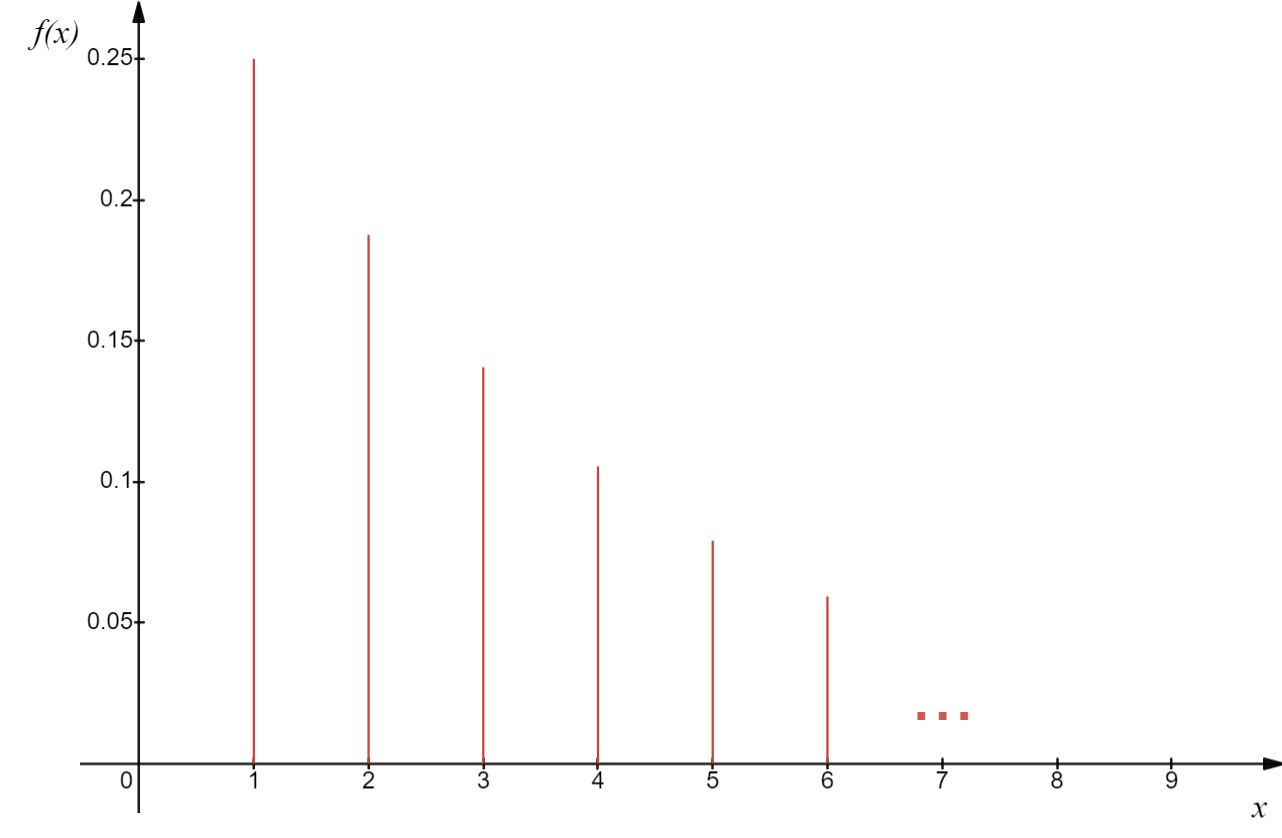
\includegraphics[width=0.75\linewidth]{./figures/geo_pdf} 

}

\caption{A geometric distribution}\label{fig:geomdriving}
\end{figure}

The choice of \(\frac{1}{4}\) is infact arbitrary. In general you can have `success' probability \(\pi\) and `failure' probability \(1-\pi\).

\begin{definition}
A random variable \(X\) representing the number of independent trials until the first success follows a geometric distribution with success probability \(\pi\), written as \(X \sim \text{Geom}(\pi)\), defined by the probability mass function

\begin{equation*}
  f(x)=\begin{cases}
    \left( 1-\pi \right)^{x-1}\pi , & x = 1, 2, 3, \dots \\
    \ 0 \ & \text{otherwise}.
  \end{cases}
\end{equation*}
\end{definition}

Of course the trials for the archer are arguably not independent - why?

\hypertarget{properties-of-probability-mass-functions}{%
\section{Properties of probability mass functions}\label{properties-of-probability-mass-functions}}

For a random variable \(X\) with probability distribution \(f(x)\) we have the following two properties:

\begin{enumerate}
\def\labelenumi{\arabic{enumi}.}
\item
  The probability of any particular value is between \(0\) and \(1\). That is,
  \[ 0 \leq f(x) \leq 1, \ \forall x\]
\item
  The probabilities sum to unity. That is,
\end{enumerate}

\[ \sum_{x} f(x)= 1\]

Probability distributions can be represented in a variety of different ways. In practice we use tables of distributions or use computer functions to evaluate them.

In R we can use the following functions to evaluate the probabilities from example \ref{exm:archer}.

\begin{Shaded}
\begin{Highlighting}[]
\NormalTok{y <-}\StringTok{ }\KeywordTok{dgeom}\NormalTok{(}\DataTypeTok{x =} \DecValTok{1}\OperatorTok{:}\DecValTok{4}\NormalTok{, }\CommentTok{#these are the particular values 1,2,3 and 4}
           \DataTypeTok{prob =} \DecValTok{1}\OperatorTok{/}\DecValTok{4}\NormalTok{ ) }\CommentTok{#This is the probability of success}
\NormalTok{y}
\end{Highlighting}
\end{Shaded}

\begin{verbatim}
## [1] 0.18750000 0.14062500 0.10546875 0.07910156
\end{verbatim}

\begin{Shaded}
\begin{Highlighting}[]
\CommentTok{#You can output these as fractions using the MASS library}
\NormalTok{MASS}\OperatorTok{::}\KeywordTok{fractions}\NormalTok{(y)}
\end{Highlighting}
\end{Shaded}

\begin{verbatim}
## [1]    3/16    9/64  27/256 81/1024
\end{verbatim}

The important function is \(\texttt{dgeom()}\), the \(\texttt{d}\) stands for distribution and \(\texttt{geom}\) for the geometric distribution.

Another way to represent a probability distribution is as a cumulative sum.

\begin{definition}[Cumulative distribution function]
Given a random variable \(X\) and its probability mass function \(f(x)\), the cumulative distribution function (abbreviated CDF) denoted with a capital letter \(F(x)\) is defined as the sum of the probabilities less than or equal to the value \(x\). That is,

\[ F(x) = \text{P}(X\leq x) = \sum_{t\leq x}f(t)\]
\end{definition}

\begin{example}[another urn problem]
Consider the setup previously where two balls numbered \(1\) through \(5\) are drawn and the maximum of two numbers is taken.
We found the probability distribution to be,

\begin{longtable}[]{@{}cc@{}}
\toprule
\(x\) & \(\text{P}(X=x)\)\tabularnewline
\midrule
\endhead
2 & \(\frac{1}{10}\)\tabularnewline
3 & \(\frac{2}{10}\)\tabularnewline
4 & \(\frac{3}{10}\)\tabularnewline
5 & \(\frac{4}{10}\)\tabularnewline
\bottomrule
\end{longtable}

Work out the CDF \(F(x)\).

\emph{solution}

If \(x<2\) we have \(F(x)=0\).
If \(2\leq x < 3\) we have \(F(x) = \frac{1}{10}\).
If \(3\leq x < 4\) we have \(F(x) = \frac{1}{10} + \frac{2}{10}\).
If \(4\leq x < 5\) we have \[F(x) = \frac{1}{10} + \frac{2}{10} + \frac{3}{10}.\]
If \(5\leq x\) we have \[F(x) = \frac{1}{10} + \frac{2}{10} + \frac{3}{10} + \frac{4}{10}.\]

Altogether,

\begin{equation*}
  F(x)=\begin{cases}
  0  \ \ \ \ \ \ \ \ \ \ \   x<2 \\
  \frac{1}{10} \  \  2\leq x < 3 \\
  \frac{3}{10} \ \  3\leq x < 4 \\
  \frac{6}{10} \ \ \ 4\leq x < 5 \\
  1 \ \ \  \ \ \  5\leq x
  \end{cases}
\end{equation*}
\end{example}

\begin{example}
The CDF of a geometric distribution is given by
\[F(x) = 1- (1-\pi)^{x}.\]
\end{example}

\emph{solution}

\[F(x) = \sum_{t\leq x}f(t)\]
Sum from \(t=1\) to \(t=x\).

\[  = \pi + \pi(1-\pi) + \pi(1-\pi)^2 + \dots +  \pi(1-\pi)^{x-1} \]
You might recognise a geometric series here, with \(a=\pi\) and \(r=(1-\pi)\), so this can be collected as:

\[F(x) = \frac{\pi (1-(1-\pi)^x)}{1-(1-\pi)} \]
Evaluating the denominator and cancelling gives the result.

The CDF is more useful than the mass function since if we are given the CDF we can calculate the mass function directly as the difference.

\[f(x) = F(x)-F(x-1)\]

\begin{example}
Calculate \(f(4)\) given the CDF

\begin{equation*}
  F(x)=\begin{cases}
  0  \ \ \ \ \ \ \ \ \ \ \   x<2 \\
  \frac{1}{10} \  \  2\leq x < 3 \\
  \frac{3}{10} \ \  3\leq x < 4 \\
  \frac{6}{10} \ \ \ 4\leq x < 5 \\
  1 \ \ \  \ \ \  5\leq x
  \end{cases}
\end{equation*}

\emph{solution}

\(f(4) = F(4)-F(3) = \frac{6}{10}-\frac{3}{10} = \frac{3}{10}\)
\end{example}

Due to the fact that the mass function can be calculated from the CDF, statistical tables often prioritise tabulating the CDF for various different types of distribution.

We finish this section with an example of how this theory may be used in applied calculations.

\begin{example}

Assuming the archer's attempts to hit a target follows a geometric distribution with success parameter \(\frac{1}{4}\) calculate the probability that he

\begin{enumerate}
\def\labelenumi{\arabic{enumi}.}
\item
  Hits on the \(10^{\text{th}}\) attempt.
\item
  Takes fewer than \(4\) attempts to hit the target.
\item
  Takes at least \(8\) attempts to hit the target.
\item
  Takes between \(4\) and \(8\) attempts inclusive.
\end{enumerate}

\end{example}

\emph{solution}

Let \(Y\) be the number of attempts to hit the target. We know that

\[f(y) = \left( \frac{3}{4} \right) ^{y-1}\frac{1}{4}\]

and

\[ F(y) = 1- \left(1-\frac{1}{4}\right)^y = 1-\left( \frac{3}{4}\right)^y.\]

\begin{enumerate}
\def\labelenumi{\arabic{enumi}.}
\item
  \(\text{P}(Y=10) = f(10) = \left( \frac{3}{4}\right)^9\times \frac{1}{4} = 0.0188\) (\(3\) s.f.).
\item
  \(\text{P}(Y<4) = \text{P}(Y\leq 3) = F(3) =1 - \left( \frac{3}{4}\right)^3 = 0.578\), (\(3\) s.f.).
\item
  Using the complement, \(\text{P}(Y\geq 8) = 1 - \text{P}(Y\leq 7)\). Now using the CDF:
\end{enumerate}

\[1-F(7) = 1- \left( 1-\left(\frac{3}{4}\right)^7\right) = 0.134.\]

\begin{enumerate}
\def\labelenumi{\arabic{enumi}.}
\setcounter{enumi}{3}
\tightlist
\item
  Rewrite the required range as a difference of two CDF values as follows:
\end{enumerate}

\[\text{P}(4\leq Y\leq 8) = \text{P}(Y\leq 8) - \text{P}(Y\leq 3)\]

\[ = F(8) - F(3)\]

\[ = \left[ 1-\left(\frac{3}{4}\right)^8\right] -  \left[ 1-\left(\frac{3}{4}\right)^3\right]\]
\[ = 0.322\]
You should be careful when evaluating the CDF to ensure that you have the correct values in the given inequality. A small diagram or list can be invaluable here.

\hypertarget{mean-variance-and-moments}{%
\section{Mean, variance and moments}\label{mean-variance-and-moments}}

The mean and variance of a random variable essentially mirror the definitions of mean and variance for samples.The mean or expected value is the \emph{average} value of the variable if it were observed repeatedly. The variance indicates the likely spread of values of the variable.

\begin{example}
If you toss a coin \(2\) times how many heads would you expect to turn up?

\emph{solution}

Your would expect \(1\) intuitively. Let \(X\) be the number of heads.
The outcomes are \((T,T),(H,T),(T,H),(H,H)\). The average number of heads is then

\[ \frac{0+1+1+2}{4} = 1\]
We can relate this to the probability of each number of heads. We have,

\[\text{P}(X=0) = \frac{1}{4}\]
\[\text{P}(X=1) = \frac{2}{4}\]
\[\text{P}(X=2) = \frac{1}{4}\]

The sum of the possible \(x\) values weighted by the probability is:
\[0\times \frac{1}{4} + 1\times \frac{2}{4} + 2\times \frac{1}{4} = 1.\]
\end{example}

\begin{definition}
The \textbf{\emph{expectation}}, or \textbf{\emph{expected value}} of a random variable \(X\) is defined as the sum of the possible values of the random variable weighted by the probability of that value.

\[ \text{E}[X] = \sum_x x\times\text{P}(X=x)\]
This is just a number once it is calculated is called the \textbf{\emph{mean}}, and so is written as a constant \(\text{E}[X]=\mu\) to omit the random quantity \(X\).

The expected value of any function of a discrete random variable \(g(X)\) is defined similarly by
\[ \text{E}[X] = \sum_x g(x)\times\text{P}(X=x)\]
\end{definition}

\begin{definition}
The \textbf{\emph{variance}} of a random variable \(X\) is defined as:

\[ \text{Var}[X] = \text{E}[(X-\mu)^2]\]
\end{definition}

The following is a very useful in practice for actually computing the variance.

\begin{theorem}
Given a random variable \(X\) we have that the variance is equal to the difference between the expectation of \(X^2\) and the squared expectation of \(X\). That is,

\[ \text{Var}[X]=\text{E}[X^2]-\text{E}[X]^2 \]
\end{theorem}

We omit the proof for now and see some examples, leaving this for the interested reader.

\begin{proof}
The expectation is a sum, so behaves linearly. By definition,

\[\text{Var}[X] = \text{E}[(X-\mu)^2]\]
Expanding out the bracket on the inside gives,
\[ = \text{E}[X^2 - 2\mu X +\mu^2] \]
Using linearity,

\[= \text{E}[X^2]-2\mu\text{E}[X]+\mu^2.\]
\[= \text{E}[X^2]-2\mu^2+\mu^2.\]
Hence the result.
\end{proof}

\begin{example}

A discrete random variable \(X\) representing the score on a loaded die has the following probability mass function.

\begin{longtable}[]{@{}cllllll@{}}
\toprule
\begin{minipage}[b]{0.28\columnwidth}\centering
\(x\)\strut
\end{minipage} & \begin{minipage}[b]{0.09\columnwidth}\raggedright
1\strut
\end{minipage} & \begin{minipage}[b]{0.09\columnwidth}\raggedright
2\strut
\end{minipage} & \begin{minipage}[b]{0.09\columnwidth}\raggedright
3\strut
\end{minipage} & \begin{minipage}[b]{0.09\columnwidth}\raggedright
4\strut
\end{minipage} & \begin{minipage}[b]{0.09\columnwidth}\raggedright
5\strut
\end{minipage} & \begin{minipage}[b]{0.09\columnwidth}\raggedright
6\strut
\end{minipage}\tabularnewline
\midrule
\endhead
\begin{minipage}[t]{0.28\columnwidth}\centering
\(\text{P}(X=x)\)\strut
\end{minipage} & \begin{minipage}[t]{0.09\columnwidth}\raggedright
\(\frac{1}{21}\)\strut
\end{minipage} & \begin{minipage}[t]{0.09\columnwidth}\raggedright
\(\frac{2}{21}\)\strut
\end{minipage} & \begin{minipage}[t]{0.09\columnwidth}\raggedright
\(\frac{3}{21}\)\strut
\end{minipage} & \begin{minipage}[t]{0.09\columnwidth}\raggedright
\(\frac{4}{21}\)\strut
\end{minipage} & \begin{minipage}[t]{0.09\columnwidth}\raggedright
\(\frac{5}{21}\)\strut
\end{minipage} & \begin{minipage}[t]{0.09\columnwidth}\raggedright
\(\frac{6}{21}\)\strut
\end{minipage}\tabularnewline
\bottomrule
\end{longtable}

Calculate:

\begin{enumerate}
\def\labelenumi{\alph{enumi})}
\item
  \(\text{E}[X]\)
\item
  \(\text{E}[X^2]\)
\item
  \(\text{Var}[X]\)
\item
  \(\text{E}[e^X]\)
\end{enumerate}

\end{example}

\emph{solution}

\begin{enumerate}
\def\labelenumi{\alph{enumi})}
\tightlist
\item
  Using the definition of expectation:
\end{enumerate}

\[ \text{E}[X] = 1\times \frac{1}{21}+2\times \frac{2}{21}+3\times \frac{3}{21}+4\times \frac{4}{21}+5\times \frac{5}{21}+6\times \frac{6}{21},\]
\[ = 4.33 \ \ \ (3 \ \text{s. f.})\]
Compared to a fair die, the mean of the loaded die is higher.

\begin{enumerate}
\def\labelenumi{\alph{enumi})}
\setcounter{enumi}{1}
\tightlist
\item
  \[ \text{E}[X^2] = 1^2\times \frac{1}{21}+2^2\times \frac{2}{21}+3^2\times \frac{3}{21}+4^2\times \frac{4}{21}+5^2\times \frac{5}{21}+6^2\times \frac{6}{21},\]
\end{enumerate}

\[ = 21\]

\begin{enumerate}
\def\labelenumi{\arabic{enumi}.}
\setcounter{enumi}{2}
\tightlist
\item
  The variance is then,
\end{enumerate}

\[\text{Var}[X]=\text{E}[X^2]-\mu^2 = 21-(4.33\dots)^2= 2.22 \ \ \ (3 \ \text{s. f.})\]
4. \(e^X\) is just a function of \(X\).

\[ \text{E}[X] = e^1\times \frac{1}{21}+e^2\times \frac{2}{21}+e^3\times \frac{3}{21}+e^4\times \frac{4}{21}+e^5\times \frac{5}{21}+e^6\times \frac{6}{21},\]

\[ = 164.622 \ (3 \ \text{d. p.}) \]

\begin{example}[expected profit]
Consider the following game. A spinning wheel is divided into three equal sections numbered \(1\), \(2\) and \(3\). You pay £\(1\) to play the game, and you have to guess the number that will show when the wheel is spun. If you guess correctly, you get £\(2\). If you do not then you get nothing. What is the expected profit from playing the game?

\emph{solution}

The profit is the winnings minus the stake. Let the profit be the random variable \(X\). The distribution of \(X\) is:

\begin{longtable}[]{@{}cllllll@{}}
\toprule
\(x\) & -1 & 1 & & & &\tabularnewline
\midrule
\endhead
\(\text{P}(X=x)\) & \(\frac{2}{3}\) & \(\frac{1}{3}\) & & & &\tabularnewline
\bottomrule
\end{longtable}

\[\text{E}[X] = -1 \times \frac{2}{3} + 1 \times \frac{1}{3} = -\frac{1}{3}\]
So we would expect on average to make a loss playing this game. For any gambling game to be profitable for the house, it is necessary that the expectation of the players winnings be negative.
\end{example}

\begin{example}
Let \(X\) be a random variable whose value is a constant, that is the particular values it can take are all the same, \(x=a\). Show that \(\text{E}[X]=a\) and \(\text{Var}[X]=0\)

\emph{solution}

\[\text{E}[X]=\sum_{x}x\times\text{P}(X=x)= \sum a\times\text{P}(X=a)=a\times \sum \text{P}(X=a) = a \times 1 = a\]

For the variance,

\[ \text{Var}[X] = \text{E}[(X-\mu)^2]=\text{E}[(a-a)^2]=0 \]
\end{example}

We will now proceed to find the mean and variance of a Geometric distribution. We will need a fact about series first.

\begin{proposition}
Suppose \(|r|<1\) and recall the infinite geometric series is given by the following formula:

\[g(r) = \sum_{k=0}^{\infty}ar^{k} = \frac{a}{1-r}\]
For a convergent series such as this we can differentiate term by term with respect to \(r\), and equate this to what we would get from differentiating the RHS likewise. Doing so results in the following two formulae:

\[g'(r) = \sum_{k=0}^{\infty}akr^{k-1} = \frac{a}{(1-r)^2}\]

\[g''(r) = \sum_{k=0}^{\infty}ak(k-1)r^{k-2} = \frac{2a}{(1-r)^3}\]
\end{proposition}

\begin{theorem}
Let \(X\) be a random variable which follows a geometric distribution, \(X \thicksim \text{Geom}(\pi)\), then we have:

\[\text{E}[X] = \frac{1}{\pi}\]
and
\[ \text{Var}[X]=\frac{1-\pi}{\pi^2}\]
\end{theorem}

\begin{proof}
By definition,
\[\text{E}[X] = \sum_{x=1}^{\infty}x(1-\pi)^{x-1}\pi\]
\[ = \pi + 2\pi(1-\pi) + 3\pi(1-\pi)^2+4\pi(1-\pi)^3+ \dots \]
The latter sum can be seen as \(g'(1-\pi)\), with \(a=\pi\). Using the RHS result from the previous proposition we have,
\[\text{E}[X] = \frac{\pi}{[1-(1-\pi)]^2} = \frac{1}{\pi}\]
For the variance we first find the expectation of a function of \(X\) called a factorial moment.

\[\text{E}[X(X-1)] = \sum_{x=1}^{\infty}x(x-1)\pi(1-\pi)^{x-1}\]
\[ = (1-\pi)\sum_{x=2}^{\infty}x(x-1)\pi(1-\pi)^{x-2}\]
The infinite series turns out to be \(g''(1-\pi)\) with \(a=\pi\). Substituting this in gives,

\[\text{E}[X(X-1)]=(1-\pi)\frac{2\pi}{[1-(1-\pi)]^3} = \frac{2(1-\pi)}{\pi^2}.\]
Now we can use this to find the variance as follows,

\[\text{Var}[X] = \text{E}[X^2]-\text{E}[X]^2 \]
\[ = \text{E}[X(X-1)]+\text{E}[X]-\text{E}[X]^2 \]
\[ = \frac{2(1-\pi)}{\pi^2} + \frac{1}{\pi} - \frac{1}{\pi^2} \]
\[ = \frac{1-\pi}{\pi^2}\]
as required.
\end{proof}

If you are given two random variables \(X\) and \(Y\) a \emph{linear combination} means an expression of the form \(aX+bY\).

\begin{theorem}[Linear Combinations]
For any random variables \(X\) and \(Y\) and constants \(a\) and \(b\) we have that the expectation of a linear combination is a linear combination of the expectations.

\[\text{E}[aX\pm bY] = a\text{E}[X]\pm b\text{E}[Y]\]
However the variance is a nonlinear sum of the variances.\\
\[\text{Var}[aX\pm bY] = a^2\text{Var}[X]+b^2\text{Var}[Y] \]
\end{theorem}

\begin{proof}
This is omitted, but follows from properties of summations and mass functions.
\end{proof}

\begin{example}
Recall the loaded die had mass function given by,

\begin{longtable}[]{@{}cllllll@{}}
\toprule
\begin{minipage}[b]{0.28\columnwidth}\centering
\(x\)\strut
\end{minipage} & \begin{minipage}[b]{0.09\columnwidth}\raggedright
1\strut
\end{minipage} & \begin{minipage}[b]{0.09\columnwidth}\raggedright
2\strut
\end{minipage} & \begin{minipage}[b]{0.09\columnwidth}\raggedright
3\strut
\end{minipage} & \begin{minipage}[b]{0.09\columnwidth}\raggedright
4\strut
\end{minipage} & \begin{minipage}[b]{0.09\columnwidth}\raggedright
5\strut
\end{minipage} & \begin{minipage}[b]{0.09\columnwidth}\raggedright
6\strut
\end{minipage}\tabularnewline
\midrule
\endhead
\begin{minipage}[t]{0.28\columnwidth}\centering
\(\text{P}(X=x)\)\strut
\end{minipage} & \begin{minipage}[t]{0.09\columnwidth}\raggedright
\(\frac{1}{21}\)\strut
\end{minipage} & \begin{minipage}[t]{0.09\columnwidth}\raggedright
\(\frac{2}{21}\)\strut
\end{minipage} & \begin{minipage}[t]{0.09\columnwidth}\raggedright
\(\frac{3}{21}\)\strut
\end{minipage} & \begin{minipage}[t]{0.09\columnwidth}\raggedright
\(\frac{4}{21}\)\strut
\end{minipage} & \begin{minipage}[t]{0.09\columnwidth}\raggedright
\(\frac{5}{21}\)\strut
\end{minipage} & \begin{minipage}[t]{0.09\columnwidth}\raggedright
\(\frac{6}{21}\)\strut
\end{minipage}\tabularnewline
\bottomrule
\end{longtable}

Suppose you win \(W\) is an amount depending on the number that you roll on the loaded die.

If \(W = 3X-10\) find \(\text{E}[W]\) and \(\text{Var}[W]\)

\emph{solution}

\[\text{E}[W] = 3\times (4.333\dots) -10 = £3\]

\[\text{Var}[W] = 3^2\times(2.22\dots) = 19.99\dots = 20.0 \  (3 \ \text{s.f.})\]
\end{example}

\hypertarget{exercises-week-3}{%
\section{Exercises Week 3}\label{exercises-week-3}}

\begin{exercise}

An urn contains two yellow balls and three red balls. Three balls are drawn at random from the urn without replacement.

\begin{enumerate}
\def\labelenumi{\alph{enumi})}
\item
  Draw a tree diagram to represent the sample space for this experiment and find the probabilities of each outcome.
\item
  Let the random variable \(X\) denote the number of red balls drawn.
\item
  Write down the probability distribtion of \(X\).
\end{enumerate}

\begin{enumerate}
\def\labelenumi{\roman{enumi})}
\setcounter{enumi}{1}
\tightlist
\item
  Find the mean and variance of \(X\).
\end{enumerate}

\end{exercise}

\begin{exercise}

Let \(X\) be the value observed from rolling an \(8\)-sided die

\begin{enumerate}
\def\labelenumi{\alph{enumi})}
\item
  What is the probability distribution of \(X\).
\item
  Draw a graph of the probability distribution.
\item
  Find the mean and variance of \(X\).
\item
  Find the expected value of:
\item
  \(3X+5\)
\end{enumerate}

\begin{enumerate}
\def\labelenumi{\roman{enumi})}
\setcounter{enumi}{1}
\tightlist
\item
  \(\ln(X)\)
\end{enumerate}

\end{exercise}

\begin{exercise}

A game consists of tossing a coin until the first head appears. The score recorded is the number of tosses required.

\begin{enumerate}
\def\labelenumi{\alph{enumi})}
\item
  If the random variable \(Y\) is the number of tosses, what is the distribution of \(Y\)?
\item
  Write down the first \(6\) values of the probability distribution, and draw a sketch.
\item
  Find the mean and variance of \(Y\).
\end{enumerate}

\end{exercise}

\begin{exercise}

Two fair dice are rolled and the \emph{total} score observed.

\begin{enumerate}
\def\labelenumi{\alph{enumi})}
\item
  Write down the probability distribution of the total score.
\item
  Find the mean and variance of the total score.
\end{enumerate}

\end{exercise}

\begin{exercise}

Two fair dice are rolled and the \emph{maximum} score observed.

\begin{enumerate}
\def\labelenumi{\alph{enumi})}
\item
  Write down the probability distribution of the maximum score.
\item
  Find the mean and variance of the maximum score.
\end{enumerate}

\end{exercise}

\begin{exercise}

A fair coin is tossed three times. Let \(X\) be the number of heads in the tosses minus the number of tails.
a) Find the probability distribution of \(X\)

\begin{enumerate}
\def\labelenumi{\alph{enumi})}
\setcounter{enumi}{1}
\tightlist
\item
  Find the mean and variance of \(X\).
\end{enumerate}

\end{exercise}

\begin{exercise}

The game of simple \emph{Chuck-a-luck} is played by a single player against the house. The game is conducted as follows:

The player chooses any number between \(1\) and \(6\) inclusive and places a bet of £\(1\). The banker then rolls \(2\) fair dice. If the player's number occurs \(1\) or \(2\) times, he wins £\(1\) or £\(2\) respectively. If the player's numberdoes not appear on any of the dice, he loses his £\(1\) stake. Let the random variable \(X\) denote the player's winnings in the game.

\begin{enumerate}
\def\labelenumi{\alph{enumi})}
\item
  Find the probability mass function of \(X\).
\item
  Find the expected value of the winnings, \(\text{E}[X]\).
\end{enumerate}

\end{exercise}

\begin{exercise}

The random variable \(X\) has the following probability mass function:

\begin{longtable}[]{@{}cccccc@{}}
\toprule
\(x\) & 1 & 2 & 3 & 4 & 5\tabularnewline
\midrule
\endhead
\(\text{P}(X=x)\) & \(7c\) & \(5c\) & \(4c\) & \(3c\) & \(c\)\tabularnewline
\bottomrule
\end{longtable}

\begin{enumerate}
\def\labelenumi{\alph{enumi})}
\item
  Find the value of \(c\) which makes this a valid probability mass function.
\item
  Find \(\text{E}[X]\) and \(\text{Var}[X]\).
\end{enumerate}

\end{exercise}

\begin{exercise}

The random variable \(X\) has the following probability mass function:

\begin{longtable}[]{@{}cccccc@{}}
\toprule
\(y\) & 2 & 3 & 5 & 7 & 11\tabularnewline
\midrule
\endhead
\(\text{P}(Y=y)\) & \(\frac{1}{6}\) & \(\frac{1}{3}\) & \(\frac{1}{4}\) & \(a\) & \(b\)\tabularnewline
\bottomrule
\end{longtable}

and \(\text{E}[Y]=\frac{14}{3}\)

\begin{enumerate}
\def\labelenumi{\alph{enumi})}
\item
  Find the values of \(a\) and \(b\).
\item
  Find \(\text{Var}[Y]\).
\end{enumerate}

\end{exercise}

\begin{exercise}

A fair six-sided die has `\(1\)' on one face, `\(2\)' on two faces and `\(3\)' on the remaining three faces.

\begin{enumerate}
\def\labelenumi{\alph{enumi})}
\item
  Let \(Y\) denote the score on a single roll of the die. Tabulate the mass function and calculate the mean and variance of \(Y\).
\item
  Let \(X\) be the total score on two rolls of the die. Tabulate the mass function and calculate the mean and variance of \(X\).
\end{enumerate}

\end{exercise}

\begin{exercise}
An urn contains \(n\) balls numbered \(1\) to \(n\) from which two balls are drawn simultaneously. Find the probability distribution of \(X\), the larger of the two numbers drawn. Calculate the expected value of \(X\).
\end{exercise}

\begin{exercise}

\(A\) and \(B\) play a game that involves each rolling a fair die simultaneously. Let \(X\) be the absolute difference in their scores.

\begin{enumerate}
\def\labelenumi{\alph{enumi})}
\item
  Tabulate the probability mass function of \(X\).
\item
  Find the mean and variance of \(X\).
\item
  If the value of \(X\) is \(1\) or \(2\) then \(A\) wins. If \(X\) is \(3\),\(4\) or \(5\) then \(B\) wins. If \(X\) is zero then they roll again. Find the probability that \(A\) wins on the first go. Find the probability that \(A\) wins on the second go. Find the probability that \(A\) wins on the \(r^{\text{th}}\) go.
\item
  Find the probability that \(A\) wins.
\end{enumerate}

\end{exercise}

\begin{exercise}
A discrete random variable has the following mass function

\begin{equation*}
  f(y)=\begin{cases}
    \pi \ \ \ \ \ \ \ \ \ \  y = 1 \\
    1-\pi \ \  \ y = 0 .
  \end{cases}
\end{equation*}

Where \(0<\pi<1\).This is known as the Bernoulli distribution.Find \(\text{E}[Y]\) and \(\text{Var}[Y]\)
\end{exercise}

\hypertarget{exercises-for-feedback-1}{%
\subsection{Exercises for feedback}\label{exercises-for-feedback-1}}

\begin{exercise}

Scrabble tiles for the letters of the word EXERCISES are in a bag.

\begin{enumerate}
\def\labelenumi{\alph{enumi})}
\item
  A random tile is drawn, what is the probability that it is the letter is E?
\item
  Given that the letter that is drawn from the bag is a vowel, what is the probability that it is an E?
\item
  Explain how the two questions are different in your own words, and compare the size of the probabilities in either part.
\end{enumerate}

\end{exercise}

\begin{exercise}

There are \(40\) students in a Maths class, and each are given a number \(1\) to \(40\). Separately the numbers \(1-40\) are placed in a hat and mixed randomly. The teacher will give three random students a prize. Three numbers are selected from the hat without replacement. Before the numbers are drawn the teacher guesses three numbers and writes them on the board.

\begin{itemize}
\tightlist
\item
  Work out the probability of the teacher matching \(0\), \(1\), \(2\) or \(3\) of the numbers that are drawn from the hat.
\end{itemize}

On a different occasion, the teacher has \(5\) students in his tutor group. He wants to give two prizes to the Maths students, and one to his tutor group. He will draw two numbers from his hat, and separately he will draw one of the numbers \(1-5\) from his shoe (he only has one hat). Again he writes his prediction on the board before the selection.

\begin{itemize}
\tightlist
\item
  Work out the probability of the teacher predicting \(0\), \(1\) or \(2\) Maths students, but not getting the tutee correct, and the probability of predicting \(0\), \(1\) or \(2\) Maths students and getting the tutee correct.
\end{itemize}

\end{exercise}

\begin{exercise}

A fairground game is played with \(5\) dice. The player pays £1 to play, and for every \(6\) that appears on the dice the player is rewarded with £\(6\).

\begin{enumerate}
\def\labelenumi{\alph{enumi})}
\item
  Work out the probabilities of getting \(0\),\(1\),\(2\),\(\dots\),\(5\) sixes when rolling the five dice.
\item
  If \(X\) is the profit of for the player of this game, work out the expected profit \(\text{E}[X]\).
\item
  Work out also the variance \(\text{Var}[X]\).
\item
  Explain if you think this is a good game or not.
\end{enumerate}

\end{exercise}

\begin{exercise}[Extension / Challenge]
You play a game with a standard pack of \(52\) cards. You are dealt a hand of \(3\) cards. If your hand contains a pair, you get \(3\) points. If your hand contains \(3\) of a kind, you get \(10\) points. If your hand contains neither a pair nor \(3\) of a kind you lose a point. What is the expected number of points you will score in this game?
\end{exercise}

\hypertarget{binpois}{%
\chapter{Special discrete random variables}\label{binpois}}

In this chapter you should be able to recognise contexts in which Binomial distributions arise. Calculate binomial probabilities using formulae. Use binomial tables, calculators and R to look up probabilities.

\hypertarget{the-binomial-distribution}{%
\section{The Binomial Distribution}\label{the-binomial-distribution}}

The binomial distribution is one of the most important discrete distributions and finds application in a wide number of areas.

The example to have in mind is the following:

\begin{example}[coin tossing]

Suppose you toss a coin \(10\) times and count the number of heads that are observed.

\begin{itemize}
\item
  There is fixed number of trials, here \(10\), and so a maximal number of heads we can observe.
\item
  The coin is the same, and so the probability of heads is the same throughout the process. For a fair coin this is \(\frac{1}{2}\).
\item
  The coin tosses are independent. There is no physical reason why any previous outcome may make heads more or less likely on subsequent tosses.
\item
  There are only two outcomes for a coin toss: heads or tails.
\end{itemize}

\end{example}

The binomial distribution can be used to find probabilities whenever the following conditions are met:

\begin{itemize}
\item
  The probability of observing a success in a single experiment is a fixed quantity, that is the probability is a constant \(\text{P}(\text{success}) = \pi\). (P for constant probability)
\item
  The trials are independent. (I)
\item
  The number of experiments, or trials, is a fixed number and so there is a maximum value attainable. (N for maximum number)
\item
  There are only two outcomes.(T for two outcomes)
\end{itemize}

The list of assumptions underlying the binomial model above can be summarised in the mnemonic PINT.

Although you can check the mnemonic is satisfied, it may in practicebe easier in a given situation to make an analogy with the coin tossing example. In a particular context the number could well vary, as could the definition of `success'. For example, suppose you are considering how many out of a number of men over \(50\), will suffer a heart attack in the next year. Then a `success' is a heart attack!

\hypertarget{the-binomial-mass-function}{%
\section{The binomial mass function}\label{the-binomial-mass-function}}

\begin{example}
You throw five drawing pins in the air and note if they land pin up or pin down. How many ways can two of the pins land facing up and the others land face down?

Suppose the probability a single pin lands facing up is \(0.3\), what is the probability that exactly two land facing up?

\emph{solution}

Consider this problem as a word UUDDD, how many different words can be obtained by rearrangement? The number of ways of rearranging this is \(\frac{5!}{2!}{3!} = 10\).

Note that this is one of the choice numbers \(^5C_2\). We are choosing from \(5\) things, two to be face up and so the remaining ones to be face down.

For any choice of two pins we have the same calculation for the probability. That is, \(0.3^2 \times 0.7^3\).

Altogether the probability is \(^5C_2 \times 0.3^2 \times 0.7^3\).
\end{example}

We can derive the binomial mass function in a similar way as this example.

\begin{theorem}
Suppose the random variable \(X\) satisfies the conditions of a binomial random variable, so that there are \(n\) trials with success probability \(\pi\). The mass function is given by:
\[\text{P}(X=x) = {}^nC_x \pi^{x}(1-\pi)^{n-x}\]
\end{theorem}

\begin{proof}
If the \(n\) trials result in \(x\) successes, each with probability \(\pi\), there must have also been \(n-x\) failures each with probability \((1-\pi)\). Using independence, the probability of this happening is

\[\pi ^x (1-\pi)^{n-x} \]
There are a number of ways this can happen, equal to \(^nC_x\). Hence result.
\end{proof}

\begin{example}
\protect\hypertarget{exm:fourfairdice}{}\label{exm:fourfairdice}Suppose a fair die is rolled four times. What is the probability of getting,

\begin{enumerate}
\def\labelenumi{\alph{enumi})}
\item
  exactly one six?
\item
  at most \(1\) six?
\end{enumerate}

\emph{solution}

\begin{enumerate}
\def\labelenumi{\alph{enumi})}
\tightlist
\item
  A common mistake is \(\frac{1}{6}\times \left( \frac{5}{6} \right)^3\). This is not correct - why? Because it can happen in \(^4C_1=4\) ways,
\end{enumerate}

\[4\times \frac{1}{6}\times \left( \frac{5}{6} \right)^3 = 0.386 \text{ (3 s.f.)}\]

\begin{enumerate}
\def\labelenumi{\alph{enumi})}
\setcounter{enumi}{1}
\tightlist
\item
  if \(X\) is the number of sixes, at most one means \(X \leq 1\). You could work this out by adding the two cases \(X=0\) and \(X=1\) together. One could calculate directly from the mass function as follows:
\end{enumerate}

\[^4C_0 \times \left( \frac{1}{6} \right)^0 \times \left( \frac{5}{6} \right)^4+ ^4C_1 \times \left( \frac{1}{6} \right)^1 \times \left( \frac{5}{6} \right)^3\]
Obtaining \(0.868\text{ (3 s.f.)}\).
\end{example}

Some examples of binomial probability distributions are given in the following figures.

\begin{figure}

{\centering 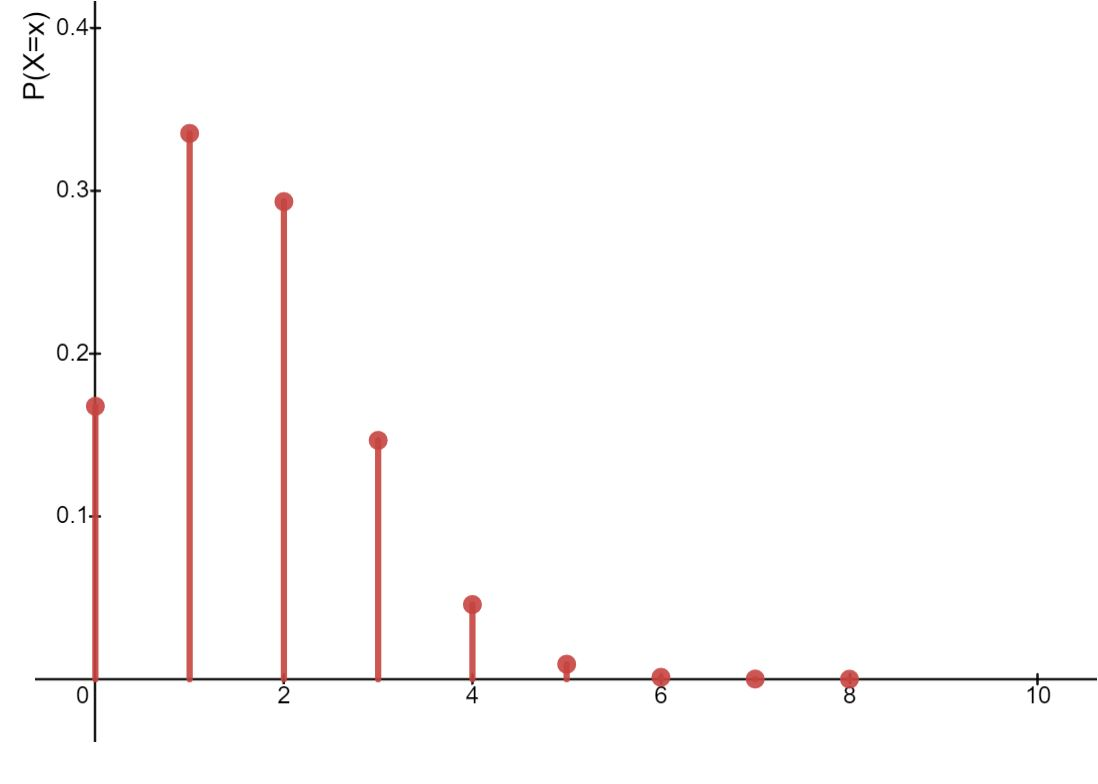
\includegraphics[width=0.75\linewidth]{./figures/binomial1} 

}

\caption{Probability mass function for B(9,0.2)}\label{fig:bin1}
\end{figure}

\begin{figure}

{\centering 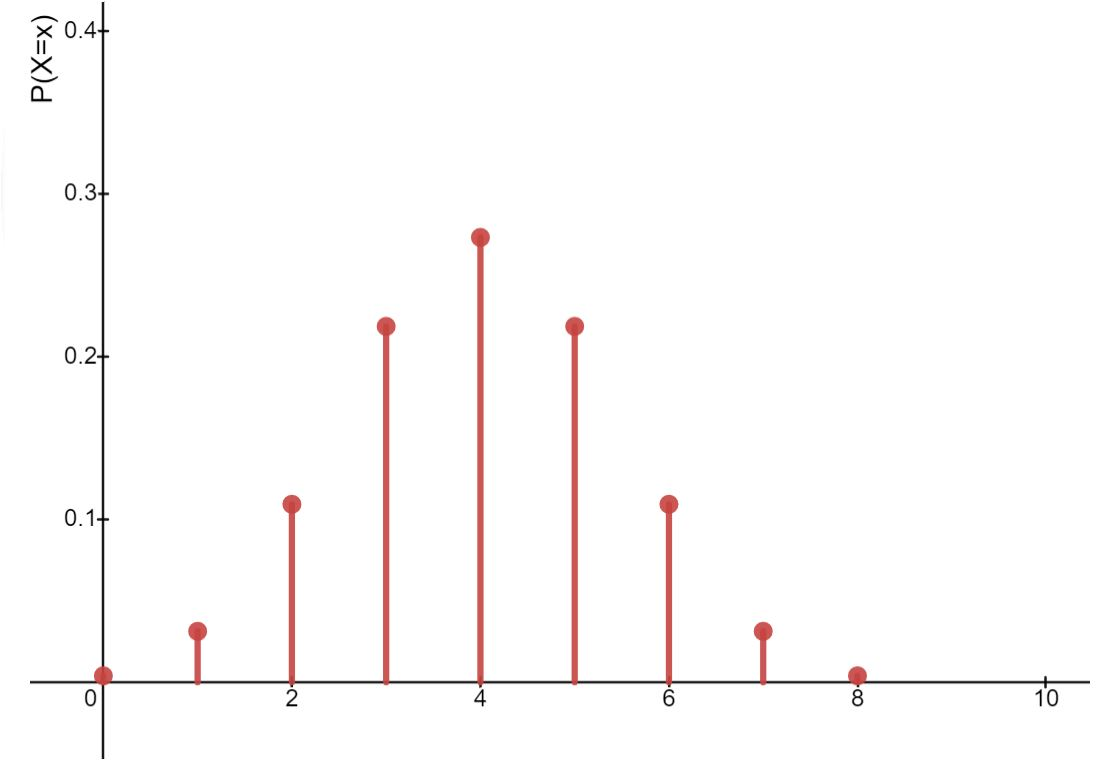
\includegraphics[width=0.75\linewidth]{./figures/binomial2} 

}

\caption{Probability mass function for B(8,0.5)}\label{fig:bin2}
\end{figure}

How can we account for the seemingly different shape?

If the success probability is close to \(0.5\) the distribution has a symmetrical shape, otherwise it is skewed.

\begin{example}
A train station has \(5\) self-service ticket machines. The probability of a machine not working at any time is \(0.15\). Let \(X\) be the number of machines not working.

\begin{enumerate}
\def\labelenumi{\alph{enumi})}
\tightlist
\item
  Comment on whether a binomial distribution is a suitable model for \(X\).
\end{enumerate}

Assuming a binomial distribution for X, evaluate the probability of the following number of machines not working.

\begin{enumerate}
\def\labelenumi{\alph{enumi})}
\setcounter{enumi}{1}
\item
  exactly \(2\).
\item
  at least \(4\).
\item
  at most \(2\).
\end{enumerate}

\emph{solution}

\begin{enumerate}
\def\labelenumi{\alph{enumi})}
\item
  Checking the mnemonic PINT here works. Here a `success' is a ticket machine not working. Independence might not hold if for example one machine not working caused the others to also fail somehow, but here the probability is the same \emph{at any time} including at a time when others have failed.
\item
  \(\text{P}(X=2) = ^5C_2 \times 0.15^2 \times (1-0.15)^{5-2} = 0.138\).
\item
  \(\text{P}(X\geq 4) = \text{P}(X=4) + \text{P}(X=5)\). Evaluating the formulae gives:
\end{enumerate}

\[= {}^5C_4 \times 0.15^4 \times (1-0.15)^{5-4}+ ^5C_5 \times 0.15^5 \times (1-0.15)^{5-5}\]
\[= 0.0022\]

\begin{enumerate}
\def\labelenumi{\alph{enumi})}
\setcounter{enumi}{3}
\tightlist
\item
  \(\text{P}(X\leq 2) = \text{P}(X=0) + \text{P}(X=1) + \text{P}(X=2)\). Again evaluating the formula for each term in the sum gives:
\end{enumerate}

\[= {}^5C_0 \times 0.15^0 \times (1-0.15)^{5-0}+ {}^5C_1 \times 0.15^1 \times (1-0.15)^{5-1}+ {}^5C_2 \times 0.15^2 \times (1-0.15)^{5-2}\]
\[ = 0.973 \]
\end{example}

Alternatively, if the number of cases to add is large enough to be tedious by hand calculation (here we only need to add a few cases together), one may consult statistical tables of the CDF.

Because the binomial distribution is so widely applied and is so important, almost every book of statistical tables will contain some pages of the binomial CDF. The tables used at MMU give probabilities for selected values of \(n\) and \(\pi\) in the form \(\text{P}(X\leq x)\). Any probability can be calculated from these tables using rules like the following:

\begin{itemize}
\item
  \(\text{P}(X\leq x)\), directly from table.
\item
  \(\text{P}(X\geq x) = 1- \text{P}(X\leq x-1)\), using complements.
\item
  \(\text{P}(X = x) = \text{P}(X\leq x) - \text{P}(X\leq x-1)\), as with getting the mass function from the CDF in the usual way.
\end{itemize}

You can the probability of \(X\) lying in a range too, but one must be careful about whether the inequality is strict or not.

\begin{itemize}
\item
  \(\text{P}(a\leq X\leq b) = \text{P}(X\leq b) - \text{P}(X\leq a-1)\)
\item
  \(\text{P}(a< X\leq b) = \text{P}(X\leq b) - \text{P}(X\leq a)\)
\item
  \(\text{P}(a\leq X < b) = \text{P}(X\leq b-1) - \text{P}(X\leq a-1)\)
\item
  \(\text{P}(a< X < b) = \text{P}(X\leq b-1) - \text{P}(X\leq a)\)
\end{itemize}

Graphing the inequality or listing the required values of \(X\) helps improve accuracy here, and I would not recommend learning just the rules here.

In modern times we more commonly would consult a calculator, which has the tables recorded in its memory. For example, in R we can do the calculation for \ref{exm:fourfairdice} using the following commands.

\begin{Shaded}
\begin{Highlighting}[]
\NormalTok{y <-}\StringTok{ }\KeywordTok{dbinom}\NormalTok{(}\DataTypeTok{x=}\DecValTok{0}\OperatorTok{:}\DecValTok{1}\NormalTok{, }\DataTypeTok{size =} \DecValTok{4}\NormalTok{, }\DataTypeTok{prob =} \DecValTok{1}\OperatorTok{/}\DecValTok{6}\NormalTok{ ) }\CommentTok{# putting x=0:1 makes y take the two values we want}
\KeywordTok{sum}\NormalTok{(y) }\CommentTok{# working out the sum is easy now}
\end{Highlighting}
\end{Shaded}

\begin{verbatim}
## [1] 0.8680556
\end{verbatim}

As with the geometric distribution, the binomial distribution function is called in R by \(\texttt{dbinom()}\), the \(\texttt{d}\) stands for distribution and \(\texttt{binom}\) for the binomial distribution.

\hypertarget{mean-and-variance}{%
\section{Mean and variance}\label{mean-and-variance}}

The goal here is to find simple expressions for the mean and variance of a binomial distribution. We choose to do this directly, though there are other methods which you may see next year.

\begin{theorem}
For a binomially distributed random variable \(X\sim \text{Bin}(n,\pi)\) we have the mean is the product of the number of trials and the success probability. That is,

\[\text{E}[X] = n\pi \]

And the variance of \(X\) is the product of the mean and the failure probability. That is,

\[ \text{Var}[X] = n\pi (1-\pi)\]
\end{theorem}

\begin{proof}
Starting with the definition,

\[ \text{E}[X] = \sum_{x=0}^{n}x\times \text{P}(X=x)\]
Combining this with the mass function gives

\[ \text{E}[X] = \sum_{x=0}^{n}x\times ^{n}C_{x} \pi^x (1-\pi)^{n-x} \]
And then the definition of the numbers \(^{n}C_{x}\),

\[ \text{E}[X] = \sum_{x=0}^{n}x\times \frac{n!}{x!\times(n-x)!} \pi^x (1-\pi)^{n-x} \]
Now the first term of the sum \(x=0\), but \(x\) is a factor of this so the sum actually starts from \(x=1\).
\[  = \sum_{x=1}^{n} \frac{n!}{(x-1)!\times(n-x)!} \pi^x (1-\pi)^{n-x} \]
\[  = n\pi\sum_{x=1}^{n} \frac{(n-1)!}{(x-1)!\times(n-x)!} \pi^{x-1} (1-\pi)^{n-x} \]
Now letting \(m=n-1\) and \(y=x-1\) the sum becomes,

\[  = n\pi\sum_{y=0}^{m} \frac{m!}{y!\times(m-y)!} \pi^{y} (1-\pi)^{m-y} \]
Each term in the sum is a binomial probability for some \(Y\sim \text{Bin}(m,\pi)\), and so altogether their sum will be equal to \(1\).

Hence \(\text{E}[X] = n\pi\).

For the variance we omit this proof as it is no longer instructive.

The interested reader could consider \(\text{E}[X(X-1)]\) and \(\text{E}[X^2]\), and the manipulations with the sums is similar to above.
\end{proof}

\hypertarget{the-poisson-distribution}{%
\section{The Poisson distribution}\label{the-poisson-distribution}}

This distribution was invented by the French mathematician Simeon Poisson, and as the distribution bears his namesake it appears capitalised unlike the binomial distribution.

The Poisson distribution can be applied in a remarkable number of areas involving counting processes. Some examples include.

\begin{itemize}
\item
  The number of `goals' scored in a sports game.
\item
  The number of sales per week.
\item
  The number of Website visitors per hour.
\item
  The number of arrivals to the A\&E of Manchester Royal Infirmary in a day.
\item
  The number of bacterial growths in a given area, such as on a Petri dish.
\end{itemize}

The Poisson distribution may be applied whenever the random variable of interest counts the number of events in a given interval, which could be any number without bound (though larger counts are less likely). The events occur one at a time, independently and randomly in the given interval. The events occur uniformly in a given interval, such that the mean number of events is proportional to the size of the interval - the events occur at a constant average rate.

The mnemonic SIR/MR can be used to summarise this paragraph.

S - not \textbf{\emph{simultaneously}}

I - Independent

R - Randomly

M - no \textbf{\emph{maximum}} number of events

R - at a constant average \textbf{\emph{rate}}

\begin{example}[telephone calls]
Let the number of telephone calls arriving at a switchboard in a minute be the random variable \(X\). Then \(X\) satisfies the assumptions to be modelled with a Poisson distribution.
\end{example}

A Poisson distribution depends on one parameter only - its mean rate \(\lambda\). Here are some pictures of Poisson distribution functions for different values of the mean rate.

\begin{figure}

{\centering 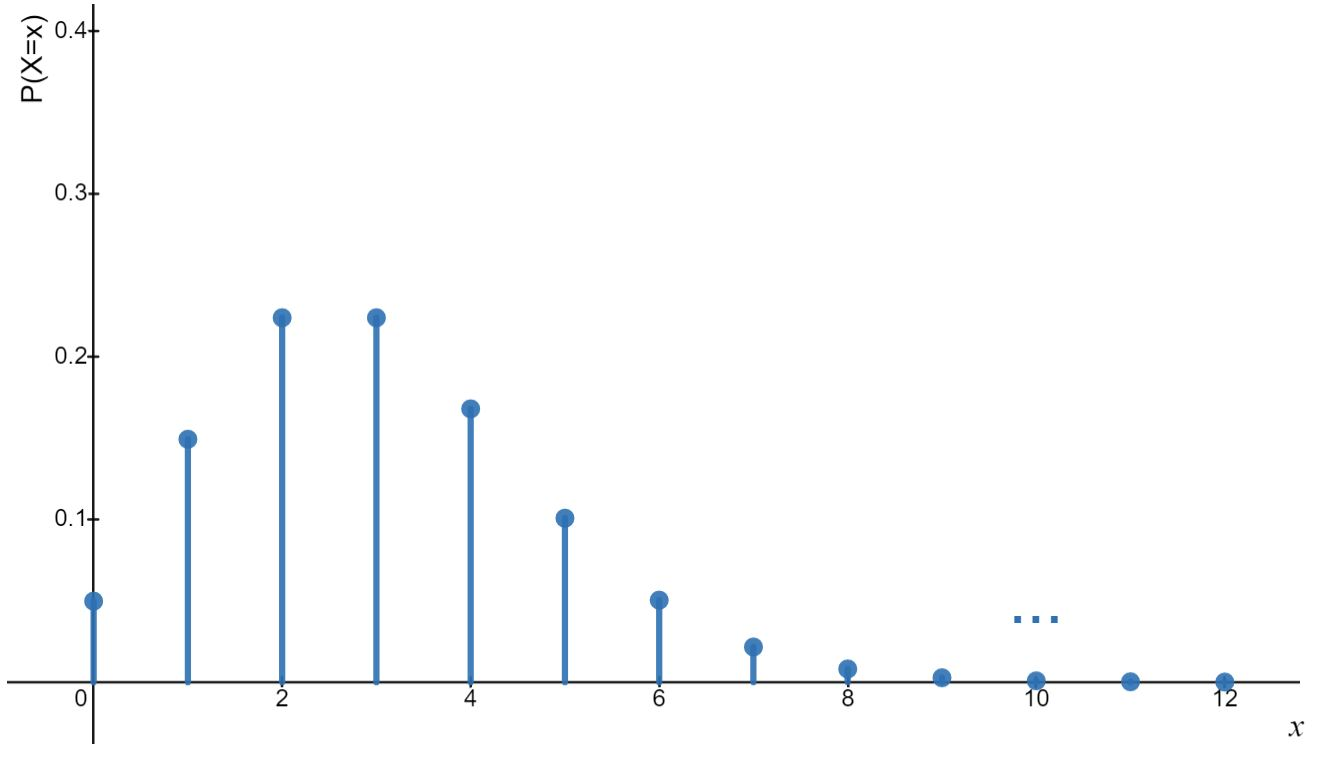
\includegraphics[width=0.75\linewidth]{./figures/poisson1} 

}

\caption{Probability mass function for Pois(3)}\label{fig:pois1}
\end{figure}

\begin{figure}

{\centering 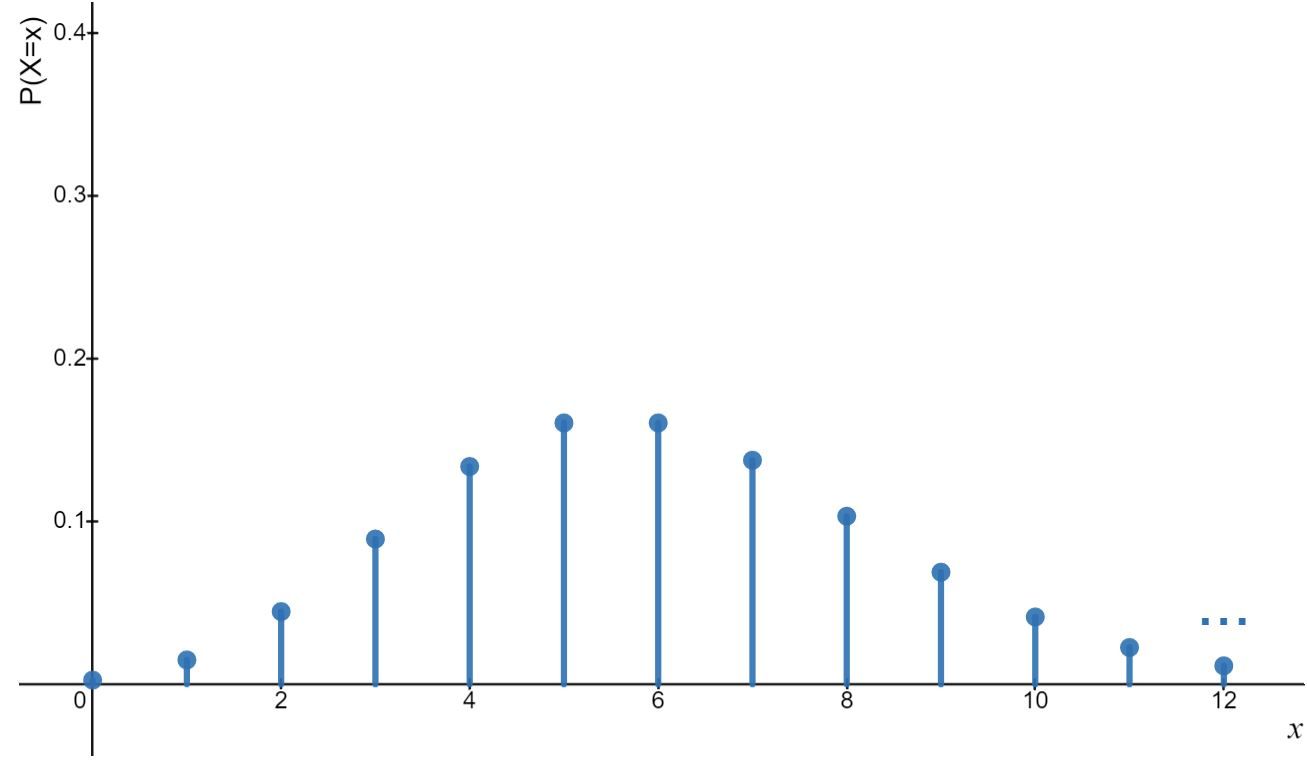
\includegraphics[width=0.75\linewidth]{./figures/poisson2} 

}

\caption{Probability mass function for Pois(6)}\label{fig:pois2}
\end{figure}

\begin{definition}
Given a random variable following a Poisson distribution \(X\sim \text{Pois}(\lambda)\) has mass function given by:

\[\text{P}(X=x) = \frac{\lambda^x e^{-\lambda}}{x!} \]
where \(x=0,1,2, \dots\), and \(\lambda>0\).
\end{definition}

Although the probabilities attached to higher values of \(x\) are positive, they quickly become very small. The mean rate \(\lambda\) does not need to be a whole number, even though the count in any given interval does need to be a whole number. As with the binomial distribution, tables are given of the CDF of the Poisson distribution.

\begin{example}

A company operates a helpdesk hotline service. Incoming calls to the hotline arrive at a mean rate of \(3.5\) per minute and outgoing calls are made at a rate of \(4.2\) per minute. Find the probability that

\begin{enumerate}
\def\labelenumi{\alph{enumi})}
\item
  at least five calls arrive in one minute.
\item
  exactly five calls arrive in one minute.
\item
  at most 7 calls are outgoing in one minute.
\item
  between \(4\) and \(9\) calls inclusive are outgoing in one minute.
\end{enumerate}

\emph{solution}

\begin{enumerate}
\def\labelenumi{\alph{enumi})}
\item
  \(\text{P}(X\geq 5) = 1 - \text{P}(X\leq 4) = 1-0.7254 = 0.2746\)
\item
  \(\text{P}(X=5) = \text{P}(X\leq 5) - \text{P}(X\leq 4) = 0.8576 - 0.7254 = 0.1322\)
\item
  \(\text{P}(Y\leq 7) = 0.9361\)
\item
  \(\text{P}(4\leq Y \leq 9 ) = \text{P}(Y\leq 9) - \text{P}(Y\leq 3) = 0.9889 - 0.3954 = 0.5935\).
\end{enumerate}

\end{example}

\hypertarget{further-properties}{%
\subsection{Further properties}\label{further-properties}}

An important aspect of the Poisson model is the uniform average rate. This means that we assume events occur at the same rate over the interval. If the size of the interval changes, then we must change the mean rate in direct proportion with that change of size.

\begin{example}[hotline continued]
Again assume calls to the hotline are incoming with rate \(3.5\) per minute. Find the probability that

\begin{enumerate}
\def\labelenumi{\alph{enumi})}
\item
  at least \(20\) calls arrive at the exchange in a \(4\) minute period.
\item
  at most \(1\) call arrives in a \(12\) second period.
\end{enumerate}

\emph{solution}

\begin{enumerate}
\def\labelenumi{\alph{enumi})}
\tightlist
\item
  If there are \(3.5\) calls per minute, then in a \(4\) minute period one expects a rate of \(3.5\times 4=14\) calls.
\end{enumerate}

Let \(W\) be the number of calls in a \(4\) minute period. Then \(W\sim\text{Pois}(14)\). Then,

\[\text{P}(W\geq 20) = 1- \text{P}(W\leq 19) = 1-0.9235 = 0.0765.\]

\begin{enumerate}
\def\labelenumi{\alph{enumi})}
\setcounter{enumi}{1}
\tightlist
\item
  As \(12\) seconds is one fifth of a minute, so we would expect a rate of \(3.5\div 5 = 0.7\) calls.
\end{enumerate}

Let \(Z\) be the number of calls in a \(12\) second period. Then,

\[\text{P}(Z\leq 1) = 0.8442\]
\end{example}

The second useful property is that different Poisson variables can be added together and yield another Poisson distribution whose rate parameter is the sum of the individual rates.

\begin{theorem}
That is, if \(X\sim \text{Pois}(\lambda)\) and \(Y\sim \text{Pois}(\mu)\) then
\[X+Y \sim \text{Pois}(\lambda+\mu)\]
\end{theorem}

\begin{proof}
Omitted for now. In your second year course you will learn moment generating functions which makes the proof very easy.
\end{proof}

\begin{example}
Suppose in a game of football the home team scores goals at a rate of \(2\) per match, and the away team scores goals at a rate of \(3\) per match. Then you would expect the total number of goals between these two teams to occur at a rate of \(5\) per match.

In this context for a particular pair of teams this may not be a realistic model. Why?
\end{example}

\hypertarget{mean-and-variance-1}{%
\section{Mean and Variance}\label{mean-and-variance-1}}

In this section we consider the mean and variance of the Poisson distribution.

We need a few Mathematical preliminaries from Calculus.

\begin{proposition}[characterisations of Euler's number]
\leavevmode

\begin{enumerate}
\def\labelenumi{\Alph{enumi})}
\tightlist
\item
  For any real number \(x \in \mathbb{R}\) we have
\end{enumerate}

\[e^x = \sum_{k=0}^{\infty} \frac{x^k}{k!}\]

\begin{enumerate}
\def\labelenumi{\Alph{enumi})}
\setcounter{enumi}{1}
\tightlist
\item
  \[ \lim_{n\to \infty} \left( 1+\frac{x}{n} \right)^n = e^x\]
\end{enumerate}

\end{proposition}

\begin{theorem}
Let \(X\) be a Poisson distributed random variable with rate \(\lambda\), that is \(X\sim \text{Pois}(\lambda)\). Then

\[\text{E}[X]  = \lambda\]
and
\[\text{Var}[X] = \lambda\]
\end{theorem}

\begin{proof}
\[\text{E}[X] = \sum_{x=0}^{\infty}x\frac{\lambda^x e^{-\lambda}}{x!}\]
\[ =\lambda e^{-\lambda} \sum_{x=1}^{\infty}\frac{\lambda^{(x-1)}}{(x-1)!} \]
\[=\lambda e^{-\lambda} \sum_{y=0}^{\infty}\frac{\lambda^{y}}{y!} \]
\[=\lambda e^{-\lambda} e^{\lambda}  \]
\[ = \lambda .\]
For the variance consider

\[\text{E}[X(X-1)] = \sum_{x=0}^{\infty}x(x-1)\frac{\lambda^x e^{-\lambda}}{x!}\]
\[ =\lambda^2e^{-\lambda} \sum_{x=2}^{\infty}\frac{\lambda^{x-2}}{(x-2)!}\]
\[ =\lambda^2e^{-\lambda} \sum_{y=0}^{\infty}\frac{\lambda^y}{y!}\]
\[ =\lambda^2e^{-\lambda} e^{\lambda}\]
\[ =\lambda^2\]
As \(\text{E}[X(X-1)] = \text{E}[X^2] - \text{E}[X]\), we can rearrange and find that

\[\text{E}[X^2] = \lambda^2 + \lambda \]

And as the variance \(\text{Var}[X] = \text{E}[X^2] - \text{E}[X]^2\), we have:

\[\text{Var}[X] = \lambda^2 + \lambda - \lambda ^2 = \lambda .\]
\end{proof}

\hypertarget{deriving-the-poisson-mass-function}{%
\section{Deriving the Poisson mass function}\label{deriving-the-poisson-mass-function}}

The Poisson distribution is intimately linked to the binomial distribution. The aim of this section is to show you why the mass function has the form given in the definition.

Suppose events occur as a result of a Poisson process independently and at a uniform rate \(\lambda\) in a given time interval. Divide up the time period into a large number of smaller intervals, \(n\) say, such that the chance of two events happening in one interval in negligible. The probability of an event happening in one of the small intervals is \(\lambda / n\).

Letting \(X\) be the random variable representing the number of small intervals that contain an event, then we can see that this is on the one hand binomially distributed for fixed \(n\). We have

\[ \text{P}(X=x) = {}^nC_{x} \left(\frac{\lambda}{n}\right)^x \left( 1- \frac{\lambda}{n}\right)^{n-x}\]

\[ = \lambda^{x} \underbrace{\frac{^nC_{x}}{n^x}}_{1} \underbrace{\left( 1- \frac{\lambda}{n}\right)^{n}}_{2}\underbrace{\left( 1- \frac{\lambda}{n}\right)^{-x}}_{3} \]

We consider what happens when we increase \(n\), and consider each term separately (which we are allowed to do for convergent sequences).

For term \(2\), as \(n\) gets larger the number inside the bracket gets close to \(1\), and so overall the limit is \(1\).

For term \(3\) this can be seen to be equal to \(e^{-\lambda}\) by the proposition (B).

The first term \(1\), can be manipulated as follows:

\[\lim_{n\to \infty}\frac{^nC_{x}}{n^x} = \lim_{n\to \infty} \frac{n!}{(n-x)!x!n^x}\]

\[ =\frac{1}{x!}  \lim_{n\to \infty} \frac{n(n-1)(n-2)\dots(n-x+1)}{n^x}\]

\[ =\frac{1}{x!}  \lim_{n\to \infty} \frac{n}{n}\frac{(n-1)}{n}\frac{(n-2)}{n}\dots \frac{(n-x+1)}{n}\]
\[ =\frac{1}{x!}  \lim_{n\to \infty} \frac{n}{n}\frac{(n-1)}{n}\frac{(n-2)}{n}\dots \frac{(n-x+1)}{n}\]
\[ =\frac{1}{x!}  \lim_{n\to \infty} \frac{(n-1)}{n}\frac{(n-2)}{n}\dots \frac{(n-x+1)}{n}\]
\[ =\frac{1}{x!}  \lim_{n\to \infty} \left(1 - \frac{1}{n}\right)\lim_{n\to \infty}\left(1 - \frac{2}{n}\right)\dots \lim_{n\to \infty} \left(1 - \frac{x-1}{n}\right)\]
And all of these limits are \(1\).

Altogether then,

\[lim_{n\to \infty} {}^nC_{x} \left(\frac{\lambda}{n}\right)^x \left( 1- \frac{\lambda}{n}\right)^{n-x}  = \lambda^x \times \frac{1}{x!} \times e^{-\lambda}\times 1 = \frac{\lambda^xe^{-\lambda}}{x!}.\]
This is the probability of observing \(x\) events in the whole time interval.

The other side of this relationship is that a Poisson distribution can be used to approximate the binomial distribution.

\begin{theorem}
If \(\pi\) is small and \(n\) is large then, a binomial distribution can be approximated by a Poisson distribution with rate parameter equal to the mean of the binomial distribution.

\[\text{Binom}(n,\pi) \approx \text{Pois} (\lambda)\]
Where we set \(\lambda = n\pi.\)

\emph{proof}
Omitted.
\end{theorem}

\hypertarget{exercises-week-4}{%
\section{Exercises week 4}\label{exercises-week-4}}

\begin{exercise}
Ropes are tested at a certain breaking strain. According to past experience a quarter of all ropes break at this strain. If \(4\) identical ropes are tested, write down the probability distribution of the number of ropes breaking.
\end{exercise}

\begin{exercise}

If it estimated that \(20\%\) of all individuals carry anibodies to a particular virus. What is the probability that in a group of \(20\) randomly selected individuals:

\begin{enumerate}
\def\labelenumi{\alph{enumi})}
\item
  More than \(8\) have antibodies.
\item
  Exactly \(6\) have antibodies.
\item
  Fewer than \(4\) have antibodies.
\item
  Between \(3\) and \(6\) inclusive have antibodies.
\end{enumerate}

\end{exercise}

\begin{exercise}

A car salesperson knows from past experience that she will make a sale to \(30\%\) of her customers. Find the probability that in \(20\) randomly selected sales pitches she makes a sale to

\begin{enumerate}
\def\labelenumi{\alph{enumi})}
\item
  More than 4 customers
\item
  Fewer than \(7\) customers
\item
  Exactly \(6\) customers
\item
  between \(4\) and \(10\) exclusive.
\end{enumerate}

\end{exercise}

\begin{exercise}
A footballer takes a free kick and scores a goal on \(10\%\) of occasions. Find the probability that in a match in which \(10\) free kicks are taken

\begin{enumerate}
\def\labelenumi{\alph{enumi})}
\item
  She scores at least two goals
\item
  She scores exactly two goals
\item
  She scores \(3\) goals or fewer.
\end{enumerate}

These are goals from free kicks alone. What assumptions do you need to make, and to what extent do you think these are reasonable?
\end{exercise}

\begin{exercise}
A statistics lecturer sets a test involving \(20\) multiple choice questions, where there are four possible answers for each question. They want to choose a pass mark so that the chance of passing a student who guesses every question is less than \(5\%\). What should the pass mark be?
\end{exercise}

\begin{exercise}
The game of \emph{advanced Chuck-a-luck} is an extension of the simple game from last week's exercises. The banker rolls \(n\) dice and the player wins £\(x\) if the number that the player guesses appears on \(x\) of the \(n\) dice. As before he loses his £\(1\) stake if the number does not come up on any of the dice.

\begin{enumerate}
\def\labelenumi{\alph{enumi})}
\item
  Write down the probability mass function of \(X\).
\item
  Show that \(\text{E}[X] = \frac{n}{6} - 1\)
\end{enumerate}

(Hint you might want to build up to part (a) in particular by picking values of \(n=1,2,3,\dots\) and pattern spotting.)
\end{exercise}

\begin{exercise}

A biologist on a field trip is studying biodiversity and has found that the number of plant species in a \(1 \  \text{m}^2\) quadrat follows a Poisson distribution with mean \(6\).

\begin{enumerate}
\def\labelenumi{\alph{enumi})}
\tightlist
\item
  Find the probability that the number of plant species in any given \(1 \  \text{m}^2\) quadrat is;
\end{enumerate}

\begin{enumerate}
\def\labelenumi{(\roman{enumi})}
\item
  at least 8
\item
  less than or equal to \(8\)
\item
  exactly \(8\)
\item
  between \(6\) and \(12\) inclusive
\end{enumerate}

\begin{enumerate}
\def\labelenumi{\alph{enumi})}
\setcounter{enumi}{1}
\tightlist
\item
  Find the probability that in a quadrat of area \(0.5 \  \text{m}^2\), the number of plant species is
\end{enumerate}

\begin{enumerate}
\def\labelenumi{(\roman{enumi})}
\item
  at least \(3\)
\item
  fewer than \(5\)
\item
  exactly \(4\)
\item
  between \(3\) and \(6\) inclusive
\end{enumerate}

\end{exercise}

\begin{exercise}

When a car leaves a production line it is carefully examined for any signs of imperfection in the paintwork. Previous experience has shown the number of blemishes per car follows a Poisson distribution with mean \(0.4\).
a) Find the probability that a car has

\begin{enumerate}
\def\labelenumi{(\roman{enumi})}
\item
  at least one blemish
\item
  more than one blemish
\item
  exactly one blemish
\item
  no blemishes
\end{enumerate}

\begin{enumerate}
\def\labelenumi{\alph{enumi})}
\setcounter{enumi}{1}
\tightlist
\item
  In \(1\) hour an inspector can examine \(20\) cars. Assuming that blemishes occur independently, find the probability that the inspector finds
\end{enumerate}

\begin{enumerate}
\def\labelenumi{(\roman{enumi})}
\item
  fewer than \(5\) blemishes
\item
  exactly five blemishes
\item
  at least one blemish
\end{enumerate}

\end{exercise}

\begin{exercise}

A traffic survey found that buses pass a checkpoint at an average rate of \(4.5\) per hour. Lorries pass the same checkpoint at the rate \(5\) per hour and coaches at the rate of \(1.5\) per hour.

\begin{enumerate}
\def\labelenumi{\alph{enumi})}
\tightlist
\item
  Find the probability that in \(1\) hour
\end{enumerate}

\begin{enumerate}
\def\labelenumi{(\roman{enumi})}
\item
  \(5\) or more buses pass the checkpoint
\item
  between \(10\) and \(15\) lorries inclusive pass the checkpoint
\item
  fewer than \(3\) buses pass the checkpoint
\end{enumerate}

\begin{enumerate}
\def\labelenumi{\alph{enumi})}
\setcounter{enumi}{1}
\item
  \begin{enumerate}
  \def\labelenumii{(\roman{enumii})}
  \tightlist
  \item
    At least \(8\) buses or coaches pass the checkpoint in an hour
  \end{enumerate}
\end{enumerate}

\begin{enumerate}
\def\labelenumi{(\roman{enumi})}
\setcounter{enumi}{1}
\item
  exactly \(15\) buses or coaches will pass the checkpoint in an hour
\item
  ten or fewer buses, lorries or coaches will pass the checkpoint in half an hour.
\end{enumerate}

\end{exercise}

\begin{exercise}

The numbers of emissions per minute from two radioactive rocks \(A\) and \(B\) are independent Poisson variables with means \(0.65\) and \(0.45\) respectively. Find the probability that

\begin{enumerate}
\def\labelenumi{(\alph{enumi})}
\item
  In a period of three minutes there are at least three emissions from \(A\).
\item
  In a period of two minutes there is a total of less than four emissions from \(A\) and \(B\) combined.
\end{enumerate}

\end{exercise}

\begin{exercise}

In a particular form of cancer, deformed blood corpuscles occur at random at the rate of \(10\) per \(1000\) corpuscles.

\begin{enumerate}
\def\labelenumi{\alph{enumi})}
\item
  Use an appropriate approximation to determine the probability that a random sample of \(200\) corpuscles taken from a cancerous area will contain no deformed corpuscles.
\item
  How large a sample should be taken in order to be \(99\%\) certain of there being at least one deformed corpuscle in the sample?
\end{enumerate}

\end{exercise}

\begin{exercise}[counting practice]

A box contains \(12\) golf balls, \(3\) of which are substandard. A random sample of \(4\) balls is selected, without replacement, from the box. The random variable \(R\) denotes the number of balls in the sample that are substandard.

\begin{enumerate}
\def\labelenumi{\alph{enumi})}
\item
\end{enumerate}

\begin{enumerate}
\def\labelenumi{(\roman{enumi})}
\tightlist
\item
  Show that the probability mass function of \(R\) satisfies
\end{enumerate}

\[\text{P}(R=r) = \frac{{}^3C_r \times {}^9C_{4-r}}{^{12}C_{4}} \]
(ii) Determine the probability that \(R=0\)

\begin{enumerate}
\def\labelenumi{(\roman{enumi})}
\setcounter{enumi}{2}
\tightlist
\item
  Determine the probability that there are fewer than two substandard balls.
\end{enumerate}

\begin{enumerate}
\def\labelenumi{\alph{enumi})}
\setcounter{enumi}{1}
\tightlist
\item
  A large bin contains \(5000\) used golf balls, \(1500\) of which are defective. The random variable \(X\) denotes the number of defective balls in a random sample of 20balls selected, without replacement,from the bin. Explain why \(X\) may be approximated as a binomial variable with parameters \(20\) and \(0.3\). Using the binomial model, calculate the probability that this sample contains
\end{enumerate}

\begin{enumerate}
\def\labelenumi{(\roman{enumi})}
\item
  fewer than \(5\) defective balls
\item
  at least \(7\) defective balls
\end{enumerate}

\end{exercise}

\begin{exercise}
The independent Poisson random variables \(X\) and \(Y\)have means \(2.5\) and \(1.5\) respectively. Obtain the mean and variance of the random variables below, and hence give a reason why they are or are not Poisson.
a) \(X-Y\)
b) \(2X+5\)
\end{exercise}

\hypertarget{cont}{%
\chapter{Continuous random variables}\label{cont}}

In this chapter we will learn about continuous random variables. Here the random variable may arise from a measurement process.

In real life many observations are assumed to take real numbered values. We could in principle observe any value on a \emph{continuum}. For example:

\begin{itemize}
\item
  The lifetime of a lithium-ion battery
\item
  The weight of a baby
\item
  The height of a random person
\end{itemize}

In practice we are constrained by the accuracy of our measuring device (heights are often quoted to the nearest inch, or centimeter) and the distinction between discrete and continuous is sometimes blurred.

\begin{example}

Consider a class of undergraduates at MMU. Each of the following is a measurement of age:

\begin{enumerate}
\def\labelenumi{\alph{enumi}.}
\item
  Age to the nearest decade
\item
  Age in years
\item
  Age in months
\item
  Age in days
\item
  Age in seconds
\end{enumerate}

\end{example}

Although none of the variables is strictly measured on a continuous scale, we would measure these variables differently. The decades would only take at most a few particular values and could be modelled as discrete, whereas age in seconds could take so many different values it's almost continuous.

\hypertarget{relation-to-histograms}{%
\section{Relation to histograms}\label{relation-to-histograms}}

Given some actual continuous data, one could make a plot how frequently the data lies within certain intervals. The resulting plot is called a histogram. These intervals need not be equal, but in modern practice they are. In most computer implementations the intervals are called bins and the interval size the bin width.

A classic example built into R is the Old Faithful geyser data. Here the waiting times between eruptions and the duration of the eruption were recorded for the Old Faithful geyser in Yellowstone National Park, Wyoming, USA.

Suppose you want to estimate a proportion or probability of a particularly long waiting time. Then instead of the bar height being equal to the frequency we can set the area to be proportional to the frequency. This can be done in such a way as to make the total area under the histogram equal to \(1\).

\begin{figure}
\centering
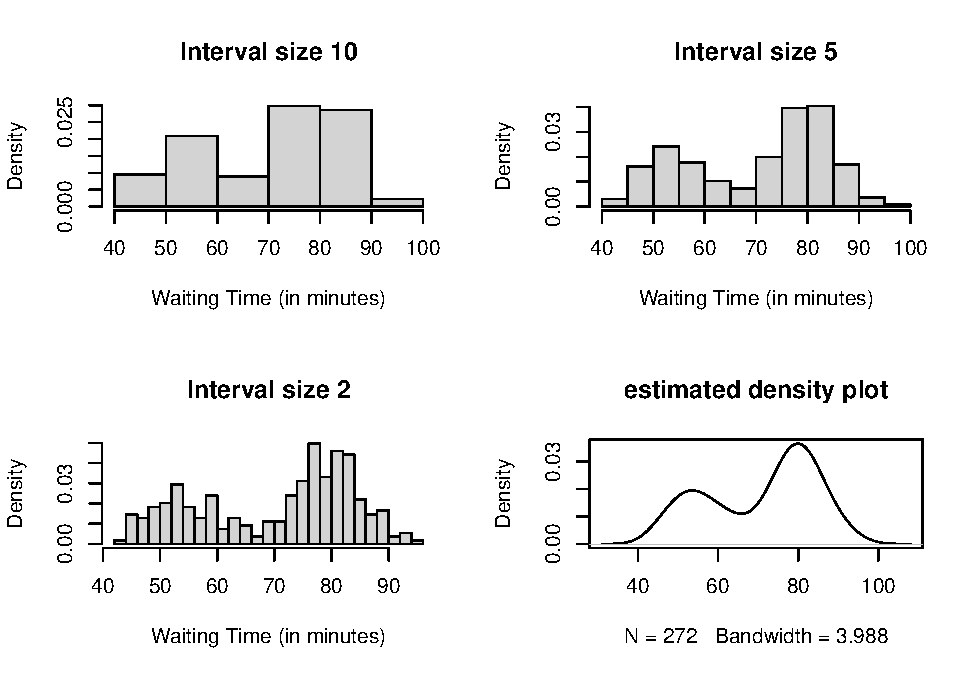
\includegraphics{6G4Z3008-notes_files/figure-latex/faithful-1.pdf}
\caption{\label{fig:faithful}Waiting time between eruptions, one sees the data in more precision with smaller bin width}
\end{figure}

To find the proportion between two values one could total the area of the bars. One can see the limit of this idea, perhaps for a very large sample is that we would have a smooth curve like the plot titled `estimated density', and find the area under the curve.

\hypertarget{two-students}{%
\section{Two students}\label{two-students}}

Consider two students who have an appointment with their tutor at \(12\)-noon.

The first student makes an effort to get there on time, so is more likely to be a little late than very late, as they live far from the university. They may be late but will certainly be there before \(1\) o'clock.
The second student has forgotten the appointment, but lives close to the university, so may arrive at any time before \(1\) o'clock, as soon as they remember.

What is the sample space here?

Take \(\Omega = [0,1]\) to be the delay measured in hours. An event here is an interval in which the student arrives. For example \([0,\frac{1}{2}]\) is the event that the student is no more than half an hour late.

The probability of arriving in a given interval is the area under the curve \[f(x) = 2-2x \ ,\ \text{for all } x\in[0,1].\]

This is shown in the image below:

\begin{figure}

{\centering 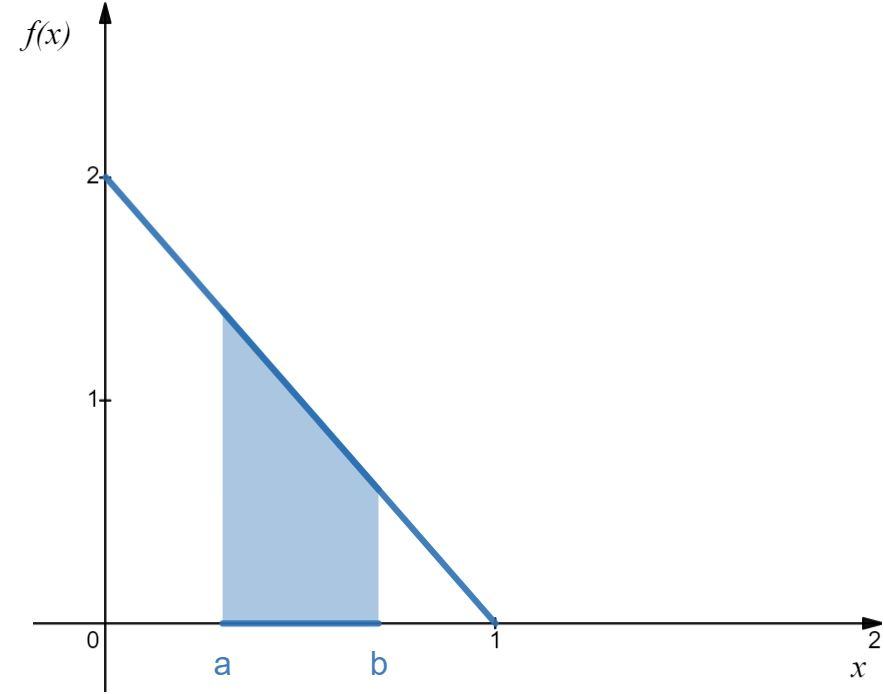
\includegraphics[width=0.75\linewidth]{./figures/student1} 

}

\caption{density function for first student}\label{fig:student1}
\end{figure}

The probability of the student arriving in the first half an hour, between \(12:00\) and \(12:30\), is \(\frac{3}{4}\), whereas the probability of arriving in the last half an hour, between \(12:30\) and \(13:00\), is \(\frac{1}{4}\).

The time until the second student arrives may be modelled by the function

\[f(x) = 1\ ,\ \text{for all } x\in[0,1].\]

This is called a \emph{uniform density} and reflects the fact that any time is equally likely.

\begin{figure}

{\centering 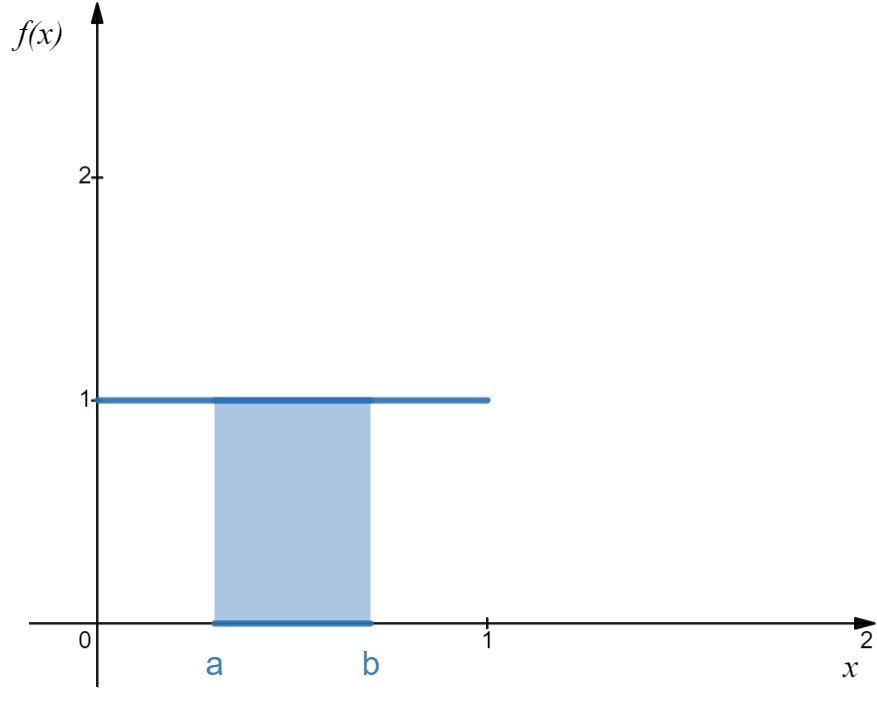
\includegraphics[width=0.75\linewidth]{./figures/student2} 

}

\caption{density function for second student}\label{fig:student2}
\end{figure}

The probability related to this function is \(\text{P}([a,b]) = b-a\).

Can you find an expression for \(\text{P}([a,b])\) for the first student?

\hypertarget{the-probability-density-function}{%
\section{The probability density function}\label{the-probability-density-function}}

For continuous random variables the equivalent of the probability mass function is called the \textbf{\emph{probability density function}}.

While for discrete random variables it makes sense to ask what is the probability that \(X\) takes some particular value \(\text{P}(X=x)\), this is always zero in the continuous setting. Instead we as what is the probability of \(X\) lying in an interval \(\text{P}(a<X<b)\).

\begin{definition}
The \textbf{\emph{probability density function}}of a continuous random variable \(X\) is a function such that

\begin{itemize}
\item
  The function is everywhere non-negative
  \[f(x) \geq 0 \text{ for all } \ x\in \mathbb{R}\]
\item
  The probability of \(X\) taking a value in the interval \((a,b)\) is given by the corresponding integral of that curve with respect to \(x\).
\end{itemize}

\[\text{P}(a<X<b) = \int_{a}^{b} f(x) \  dx\]

\begin{itemize}
\tightlist
\item
  The total area under the graph over the domain of \(f(x)\) is unity. Let the domain of \(f(x)\) be \(x\in (c,d)\).
\end{itemize}

\[ \int_{c}^{d} f(x) \  dx = 1\]
\end{definition}

\begin{example}
The continuous random variable \(X\) has probability density function given by

\begin{equation*}
  f(x)=\begin{cases}
    \frac{1}{2}x, &  0< x < 2\\
    0 & \text{otherwise}.
  \end{cases}
\end{equation*}

Calculate \(\text{P}(X>1)\).

\emph{solution}

you should do a sketch to get an intuition for whether the probability will be more than a half.

You could use calculus here, but if you draw a picture the area required is a trapezium.

The area is therefore \(\frac{(\frac{1}{2}+1)\times 1}{2}=\frac{3}{4}\).
\end{example}

\begin{example}
A continuous random variable has probability density function \(f(x) = kx^2\) for \(0\leq x\leq 4\).

\begin{enumerate}
\def\labelenumi{\alph{enumi})}
\item
  Find the value of the constant \(k\)
\item
  Find \(\text{P}(1\leq X \leq 3)\)
\end{enumerate}

\emph{solution}

\begin{enumerate}
\def\labelenumi{\alph{enumi})}
\item
\end{enumerate}

We need to use calculus here as we have a curve.

To find \(k\), we use the fact that \(f\) integrates to \(1\) over the domain.

\[ \int_{0}^{4}kx^2 \ dx = \left[ \frac{kx^3}{3}\right]^{x=4}_{x=0}\]

\[ 1= \frac{k}{3} (64-0)\]
\[ 1= \frac{64k}{3} \]
Hence \(k=\frac{3}{64}\).

\begin{enumerate}
\def\labelenumi{\alph{enumi})}
\setcounter{enumi}{1}
\tightlist
\item
  \[\text{P}(1\leq X \leq 3) = \int_{1}^{3} \frac{3}{64}x^2 \ dx\]
\end{enumerate}

Evaluating this numerically gives \(0.406\) to \(3\) significant figures.
\end{example}

Notice that if the inequality were \(1<X<3\) or any combination of \(<\) and \(\leq\) the calculation would be the same, so we do not need to worry about the inequality being strict or not for continuous random variables.

This is because the area at a single \(x\) value has zero width, so does not contribute to the integral.

\hypertarget{expectation-and-variance}{%
\section{Expectation and variance}\label{expectation-and-variance}}

The expectation is defined similarly to the case of discrete random variables, but here we use the integral rather than a sum.

\begin{definition}
The \textbf{\emph{expectation}}, or \textbf{\emph{expected value}} or \textbf{\emph{mean value}} of a continuous random variable \(X\) is given by

\[ \text{E}[X] = \int_{-\infty}^{\infty}x f(x) \ dx\]
Where the limits indicate that the integral is over the smallest and largest attainable values of \(X\). The mean value is often denotes \(\text{E}[X] = \mu\).

More generally we define

\[ \text{E}[g(X)] = \int_{-\infty}^{\infty}g(x) f(x) \ dx\]
\end{definition}

\begin{definition}
The variance of a continuous random variable is given by

\[\text{Var}[X] = \text{E}[(X-\mu)^2] = \text{E}[X^2]-\mu^2\]
The standard deviation \(\sigma\) of \(X\) is the square root of the variance. That is

\[\sigma = \sqrt{\text{Var}[X]}\]
\end{definition}

\begin{example}[marathon times]
The times in excess of \(2\) hours taken to complete a marathon road race are modelled by the continuous random variable \(T\) hours, where \(T\) has the probability density function

\begin{equation*}
  f(t)=\begin{cases}
    \frac{4}{27}t^2(3-t), &  0< x < 3\\
    0 & \ \ \ \  \text{otherwise}.
  \end{cases}
\end{equation*}

Find the \emph{mean} and \emph{standard deviation} of the times taken to complete the race.
\end{example}

\emph{solution}

For the mean

\[ \text{E}[T] = \int_{0}^{3} t\times \frac{4}{27}t^2(3-t) \ dt\]

This can be evaluated (for example numerically) as \(\frac{9}{5}\). This can be interpreted as \(1\) hour and \(48\) minutes excess of \(2\) hours, so the mean time is \(3\) hours and \(48\) minutes.

The variance use \(\text{Var}[T]=\text{E}[X^2]-\text{E}[X]^2 = \frac{18}{5} - (\frac{9}{5})^2 =\frac{9}{25}\). The interpretation is \(21.6\) minutes variance, and so \(\sigma = \sqrt{21.6} = 4.65\) minutes (\(3\) s.f.) standard deviation

\hypertarget{mode}{%
\section{Mode}\label{mode}}

If the probability density function has a unique maximum then the value of \(X\) at the maximum is called the mode. To locate the mode it is a good idea to draw a sketch. Sometimes the mode can be deduced immediately. Other times one may need to differentiate.

\begin{example}

Deduce the mode in the following cases

\begin{enumerate}
\def\labelenumi{\alph{enumi})}
\item
  \[f(x) = \frac{1}{8}x , 0\leq x \leq 4\]
\item
  \begin{equation*}
    f(x)=\begin{cases}
   \frac{1}{4}x, &  0< x \leq 2 \\
   1-\frac{1}{4}x & \ \  2< x \leq 4 \\
   0& \ \ \ \ \  \ \ \text{otherwise}
    \end{cases}
  \end{equation*}
\item
  \[f(x) = \frac{3}{80}(2+x)(4-x) , \ \  0\leq x \leq 4.\]
\end{enumerate}

\emph{solution}

\begin{enumerate}
\def\labelenumi{\alph{enumi})}
\item
  mode is 4
\item
  mode is 2
\item
  One could differentiate or complete the square here to show the mode is \(1\).
\end{enumerate}

\end{example}

\begin{example}[marathon times]
The times in excess of \(2\) hours taken to complete a marathon road race are modelled by the continuous random variable \(T\) hours, where \(T\) has the probability density function

\begin{equation*}
  f(t)=\begin{cases}
    \frac{4}{27}t^2(3-t), &  0< t < 3\\
    0 & \ \ \ \  \text{otherwise}.
  \end{cases}
\end{equation*}

Find the modal time taken to complete the race.
\end{example}

\emph{solution}

Differentiating gives

\[f'(t) = \frac{4}{27}(2t \times(3-t) + t^2\times(-1)) = \frac{4}{27}(6t -3t^2)\]

Setting \(f'(t)=0\) yields

\[0 = 3t(2 - t) \]
So either\(t=0\) or \(2\). So the modal excess is \(2\) hours, and the modal total time is \(2+2=4\) hours.

\hypertarget{cdf}{%
\section{CDF}\label{cdf}}

The cumulative distribution function can be defined in a similar way to discrete random variables.

\begin{definition}
The \textbf{\emph{distribution function}} or more simply the \textbf{\emph{CDF}} of a continuous random variable is the function defined by

\[F(x) = \text{P}(X\leq x) = \text{P}(X< x).\]

The function \(F\) is related to the density via

\[F(x) = \int_{-\infty}^{x}f(u) \ du\]
Where the lower limit \(-\infty\) is in practice the lowest attainable value of \(X\).

On the other hand,

\[ f(x) = \frac{d}{dx} F(x)\]
\end{definition}

These are some facts about the CDF.

\begin{itemize}
\item
  Since it is always impossible to have a value smaller than \(-\infty\) or larger than \(\infty\) we have \(F(-\infty)=0\) and \(F(\infty)=1\)
\item
  \(F\) is called \emph{monotonically increasing} which means it either increases or remains constant but never decreases.
\item
  \(F\) is a continuous function, even if \(f\) is not.
\item
  Useful relations are
  \[\text{P}(c<X<d) = F(d) - F(c)\]
\end{itemize}

and

\[ \text{P}(X>x) = 1-F(x)\]

\begin{example}
For a continuous random variable \(X\) with density

\[f(x) = \frac{1}{8}x, \ 0\leq x\leq 4\]
a) Find the distribution function \(F(x)\) and sketch it.

\begin{enumerate}
\def\labelenumi{\alph{enumi})}
\setcounter{enumi}{1}
\tightlist
\item
  Evaluate \(\text{P}(0.3\leq X\leq 1.8)\)
\end{enumerate}

\emph{solution}

For values between \(0\) and \(4\) we have

\[F(t) = \int_{0}^{t} \frac{1}{8}x \ dx = \left[ \frac{x^2}{16}\right]^{t}_{0}= \frac{t^2}{16}\]

Altogether

\begin{equation*}
  F(x)=\begin{cases}
        0 \ \ \ \ x\leq 0 \\
        \frac{x^2}{16} \ \ \   0\leq x \leq 4\\
        1 \ \ \ \ x\geq 4
  \end{cases}
\end{equation*}
\end{example}

\begin{example}
For a continuous random variable \(X\) with density

\begin{equation*}
  f(x)=\begin{cases}
        \frac{x}{3} \ \ \ \ \ \ \ \ \ \ \ \ 0\leq x\leq 2  \\
        -\frac{2}{3}x+2 \ \ \   2\leq x \leq 3\\
        0 \ \ \ \ \ \ \ \ \ \ \ \  \ \ \ \text{otherwise}
  \end{cases}
\end{equation*}

\begin{enumerate}
\def\labelenumi{\alph{enumi})}
\tightlist
\item
  Find the CDF F(x) and sketch it.
\end{enumerate}

\emph{solution}

The CDF must be found in two stages as \(f\) is a piecewise function.

Integrating over the interval \(0\leq x\leq 2\) gives \(\frac{x^2}{6}\)

Integrating over the interval \(2\leq x \leq 3\), and adding the integral over the previous interval, gives \(-\frac{x^2}{3} +2x -2\)

Altogether

\begin{equation*}
  F(x)=\begin{cases}
        \frac{x^2}{6} \ \ \ \ \ \ \ \ \ \ \ \ \ \ \ \ \ \ 0\leq x\leq 2  \\
        -\frac{x^2}{3} +2x -2 \ \ \   2\leq x \leq 3\\
        1 \ \ \ \ \ \ \ \ \ \  \ \ \ \ \  \ \ \ x\geq 3
  \end{cases}
\end{equation*}
\end{example}

Generally speaking a plot or sketch of \(F\) will look vaguely S-shaped.

\begin{figure}

{\centering 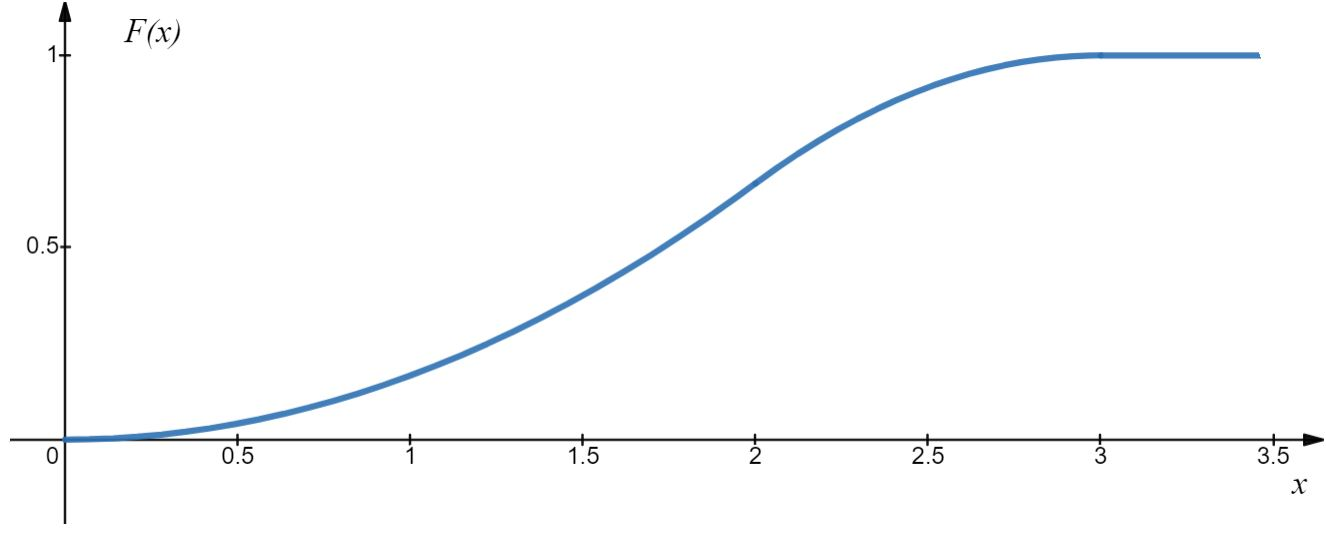
\includegraphics[width=0.75\linewidth]{./figures/cum1} 

}

\caption{cumulative distribution function is S shaped}\label{fig:cum1}
\end{figure}

For discrete random variables we sometimes called \(f\) the distribution function and called \(F\) the cumulative distribution function. However for continuous random variables \(f\) is never called the distribution function, and only called the density function, and \(F\) is called the distribution function exclusively.

\hypertarget{median-quartiles-and-percentiles}{%
\section{median, quartiles and percentiles}\label{median-quartiles-and-percentiles}}

The median, quartiles and percentiles are best expressed in terms of the CDF.

The median is the value \(50\%\) of the way through the distribution. It splits the area under the curve \(y=f(x)\) into two halves.

\begin{definition}
The \textbf{\emph{median}} of a continuous random variable \(X\) is the value \(m\) that satisfies either of

\[F(m) = 0.5 , \ \ \ \ \int_{-\infty}^{m}f(x) \ dx = 0.5\]
\end{definition}

\begin{definition}
The \textbf{\emph{lower quartile}} \(Q_1\) satisfies \(F(Q_1) = 0.25\).
The \textbf{\emph{upper quartile}} \(Q_3\) satisfies \(F(Q_3) = 0.75\).
The median is the second quartile \(m=Q_2\).
\end{definition}

\begin{definition}
More generally one may define a \textbf{\emph{percentile}} \(P_{\alpha}\) at \(\alpha \%\) to be the value such that \(F(P_{\alpha})= \alpha \%\). The median is the \(50^{\text{th}}\) percentile \(m = P_{50}\), and \(Q_1 = P_{25}\), \(Q_3 = P_{75}\)
\end{definition}

\begin{definition}
More generally still is the \textbf{\emph{quantile}} which is the value \(q\) such that \(F(q)=p\) for any \(p\in(0,1)\)
\end{definition}

\begin{example}
Let's find the median for the marathon example.

\begin{equation*}
  f(t)=\begin{cases}
    \frac{4}{27}t^2(3-t), &  0< t < 3\\
    0 & \ \ \ \  \text{otherwise}.
  \end{cases}
\end{equation*}

First find the CDF.

In the range \(0< t < 3\)
\[F(t) = \frac{4}{27}\int_{0}^{t} u^2(3-u) \ du\]

\[= \frac{4}{27}\left[\frac{3u^3}{3}-\frac{u^4}{4}\right]^{t}_{0} =\frac{4}{27}\left( t^3 - \frac{t^4}{4} \right)\]

Then solving \(F(t)=0.5\),

\[\frac{4}{27}\left(t^3 - \frac{t^4}{4} \right)= 0.5\]
this can be evaluated numerically and there are two values \(t=3.74\) and \(t= 1.84\) the first one is outside the range of \(0< t < 3\) so is discarded. And so the median time is \(2+1.84 = 3.84\) hours to complete the marathon. This is just under the mean.
\end{example}

The marathon example shows that mode, median and mean are not the same number usually. The mode was \(4\), the median was \(3.84\) and the mean was \(3.8\) hours.

\hypertarget{uniform-distribution}{%
\section{Uniform distribution}\label{uniform-distribution}}

We encountered a uniform random variable in the example of the forgetful student. Its characteristic is that for its entire domain of values of \(X\) the density is constant.

If the density is a constant on some interval, that means \(f(x) = k\) for \(a\leq x \leq b\). What is the value of \(k\)?

\begin{definition}
A continuous random variable follows a continuous \textbf{\emph{uniform distribution}} (sometimes called \textbf{\emph{rectangular}}) with support \([a,b]\), denoted \(X\sim U(a,b)\) has probability density function given by

\begin{equation*}
  f(x)=\begin{cases}
    \frac{1}{b-a}, &  a< x < b\\
    0 & \ \ \ \  \text{otherwise}.
  \end{cases}
\end{equation*}
\end{definition}

The uniform distribution is symmetrical so the mean is equal to the median, but there is no mode here.

\begin{theorem}
For a continuous uniform distribution \(X\sim U(a,b)\)

\[\text{E}[X] = \frac{a+b}{2}\]

and

\[\text{Var}[X]= \frac{(b-a)^2}{12}\]
\end{theorem}

\begin{proof}
\[\text{E}[X] = \int_a^b x \times \frac{1}{b-a} dx  =\frac{1}{b-a} \left[ \frac{x^2}{2} \right]^{b}_{a}\]

Now

\[= \frac{1}{b-a} \left( \frac{b^2-a^2}{2} \right)\]
And using the difference of two squares

\[= \frac{1}{b-a} \left( \frac{(b-a)(b+a)}{2} \right)\]
Hence the result, upon cancelling \((b-a)\).

For the variance consider

\[\text{E}[X^2] = \int_a^b x^2 \times \frac{1}{b-a} dx  =\frac{1}{b-a} \left[ \frac{x^3}{3} \right]^{b}_{a}\]

\[= \frac{1}{b-a} \left( \frac{b^3-a^3}{3} \right)\]

And using the difference of cubes

\[= \frac{1}{b-a} \left( \frac{(b-a)(b^2+ab+a^2)}{3} \right)\]

Hence \(\text{E}[X^2] = \frac{b^2+ab+a^2}{3}\).

Now

\[\text{Var}[X] = \text{E}[X^2] - \text{E}[X]^2 = \frac{b^2+ab+a^2}{3} - \left(\frac{a+b}{2} \right)^2\]

\[ = \frac{4(b^2+ab+a^2)- 3(a^2 + 2ab +b^2)}{12}\]
\[= \frac{a^2-2ab +b^2}{12}\]
Hence result by factorising the numerator.
\end{proof}

The CDF of the continuous uniform distribution can also be found.

\begin{proposition}
The CDF of a continuous uniform distribution \(X\sim U(a,b)\) has the form

\begin{equation*}
  F(x)=\begin{cases}
        0 & x \leq a \\
    \frac{x-a}{b-a}, &  a< x < b\\
    1 & \ \ x \geq b.
  \end{cases}
\end{equation*}
\end{proposition}

\emph{proof}

Find the equation of the line between \((a,0)\) and \((b,1)\).

\hypertarget{exponential-distribution}{%
\section{Exponential distribution}\label{exponential-distribution}}

The exponential distribution is like the continuous version of a geometric distribution. Instead of counting how many attempts until some event happens, we instead measure the time until an event occurs that would ordinarily occur at some rate.

Consider a sequence of independent events occuring at random points in time at a rate \(\lambda\). We learned last week how the number of events that occur could be modelled by a discrete random variable called a Poisson distribution.

Instead of counting how many events occur, we could consider measuring how long we wait until the next event.

We set a starting time \(x=0\) and denote the random variable `the time to the first event' by \(X\).

\[\text{P}(X>x) = \text{P}( \{\text{No events occur in the time interval (0,x)}\})\]

The mean number of events that occur per unit interval is \(\lambda\). So the number of events that occur in the interval \((0,x)\) of length \(x-0 = x\) is scaled proportionally so equals \(\lambda \times x\).

The probability of obtaining \(0\) events from a Poisson distribution with mean \(\lambda x\) is

\[\frac{(\lambda x)^0 e^{-\lambda x}}{0!} = e^{-\lambda x}\]
So

\[\text{P}(X>x) =  e^{-\lambda x}\]
And the cumulative distribution equals

\[F(x) = 1-\text{P(X>x)}=1-e^{-\lambda x}\]

Differentiating this with respect to \(x\) we obtain

\[f(x) = \lambda e^{-\lambda x}\]

\begin{definition}
A continuous random variable \(X\) is said to have an \textbf{\emph{exponential distribution}}, denoted \(X\sim \text{Exp}(\lambda)\) if it has the density function

\[f(x) = \lambda e^{-\lambda x} , x >0\]
\end{definition}

Now we will consider the shape of the exponential distribution.

\begin{theorem}
For an exponential distribution \(X\sim \text{Exp}(\lambda)\), we have

\[\text{E}[X] = \frac{1}{\lambda}\]
and

\[\text{Var}[X] = \frac{1}{\lambda ^2}\]
\end{theorem}

\begin{proof}
This can be verified by using integration.
\end{proof}

\hypertarget{exercises-week-5}{%
\section{Exercises week 5}\label{exercises-week-5}}

\begin{exercise}

A random variable \(Y\) has density function

\begin{equation*}
  f(x)=\begin{cases}
        ky & 0 \leq y \leq 4 \\
        0 &  \text{     Otherwise}
  \end{cases}
\end{equation*}

\begin{enumerate}
\def\labelenumi{\alph{enumi})}
\item
  Show that \(k = \frac{1}{8}\) that makes this a valid density function
\item
  Find the cumulative distribution function \(F(y)\)
\item
  Sketch the density \(f\) and \(F\) on the same axes
\item
  Calculate \(\text{P}(1\leq Y \leq 3)\) in two ways, one with \(f\) and one with \(F\).
\item
  Calculate the mean \(\text{E}[Y]\) and variance \(\text{Var}[Y]\) of \(Y\).
\end{enumerate}

\end{exercise}

\begin{exercise}

The length of time in minutes to serve a customer at a fast food restaurant is a random variable \(T\) with density

\begin{equation*}
  f(t)=\begin{cases}
        k(3t^2 + t) & 0 \leq t \leq 2 \\
        0 &  \text{     Otherwise}
  \end{cases}
\end{equation*}

\begin{enumerate}
\def\labelenumi{\alph{enumi})}
\item
  Show that \(k = \frac{1}{10}\) that makes this a valid density function
\item
  Find the cumulative distribution function \(F(t)\)
\item
  Sketch the density \(f\) and the distribution \(F\).
\item
  Use the graph of \(F\) to find the median.
\item
  Calculate the probability that the time to serve a customer is one minute or less.
\item
  Calculate the mean \(\text{E}[T]\) and variance \(\text{Var}[T]\) of the serving times.
\end{enumerate}

\end{exercise}

\begin{exercise}
Suppose the profit that a certain contractor will make on any one job, in thousands of pounds, is a random variable \(X\) with density function given by

\begin{equation*}
  f(x)=\begin{cases}
        c(4x -x^3) & 0 \leq x \leq 2 \\
        0 &  \text{     Otherwise}
  \end{cases}
\end{equation*}

\begin{enumerate}
\def\labelenumi{\alph{enumi})}
\item
  Show that \(k =\frac{1}{4}\) that makes this a valid density function
\item
  Find the expected profit and the variance of the profit per contract.
\item
  Find the cumulative distribution function \(F(x)\) and hence the median profit level.
\item
  What is the probability that the contractor makes a profit of less than £\(600\) on a contract?
\item
  Assuming that the profit levels for each contract are independent, what is the probability that the profit level is less than £\(600\) on
  i) each of the next \(10\) jobs?
  ii) exactly \(4\) of the next \(10\) jobs?
\end{enumerate}

(Hint: for part (e) you should use your answer from (d) and an appropriate binomial distribution)
\end{exercise}

\begin{exercise}

The lifetime of a mobile phone batters (in hundreds of hours) is a random variable \(X\) with density function

\begin{equation*}
  f(x)=\begin{cases}
        2xe^{-x^2} &  x \geq 0 \\
        0 &  \text{     Otherwise}
  \end{cases}
\end{equation*}

\begin{enumerate}
\def\labelenumi{\alph{enumi})}
\item
  Show that this is a valid density function (integrate by substitution)
\item
  Find the cumulative distribution function.
\item
  Find the median lifetime of the battery
\item
  Evaluate \(\text{P}(X\geq 2)\)
\end{enumerate}

\end{exercise}

\begin{exercise}

Bacteria grow on a Petri dish in a circular disk. The radius of a circle \(R\) can be modelled by a uniform distribution in the interval between \(1\) and \(3\) cm.

\begin{enumerate}
\def\labelenumi{\alph{enumi})}
\item
  Write down the density and distribution functions of \(R\)
\item
  Work out the expected value of R and the variance of \(R\).
\item
  If the area of the circle is the random variable \(A\), determine the distribution function of \(A\).
  (Start by considering what \(\text{P}(A\leq a)\) means in terms of \(R\).)
\item
  Determine the density function of \(A\).
\item
  Calculate the expected value of the area \(A\).
\end{enumerate}

\end{exercise}

\hypertarget{exercises-for-feedback-week-5}{%
\subsection{Exercises for feedback week 5}\label{exercises-for-feedback-week-5}}

\begin{enumerate}
\def\labelenumi{\arabic{enumi}.}
\tightlist
\item
  An archer continues to shoot at a target until he hits the bullseye.
\end{enumerate}

\begin{enumerate}
\def\labelenumi{\alph{enumi})}
\tightlist
\item
  Give a reason why it may be possible to model X with a geometric
  distribution.
\end{enumerate}

The archer shoots the target around \(100\) times and \(5\%\) of the shots hit the bullseye.
Suppose \(X \sim Geom(p)\) with \(p =5\%\).

\begin{enumerate}
\def\labelenumi{\alph{enumi})}
\setcounter{enumi}{1}
\item
  Calculate the probability that he shoots the target in at least ten attempts.
\item
  Give a reason why a geometric distribution may not be appropriate here, and how you could improve the model.
\end{enumerate}

\begin{enumerate}
\def\labelenumi{\arabic{enumi}.}
\setcounter{enumi}{1}
\tightlist
\item
  A continuous random variable \(X\) has the density function
\end{enumerate}

\begin{equation*}
  f(x)=\begin{cases}
        kx(1-x^2) & 0\leq x \leq 1 \\
        0 , &  \text{   otherwise}\\
  \end{cases}
\end{equation*}

\begin{enumerate}
\def\labelenumi{\alph{enumi})}
\item
  Find the value of the constant \(k\)
\item
  Calculate the mean and variance of \(X\).
\item
  Find an expression for the cumulative distribution \(F_X(x)\) and sketch this function.
\item
  Hence or otherwise calculate \(\text{P}(X\leq \frac{1}{3})\).
\end{enumerate}

\begin{enumerate}
\def\labelenumi{\arabic{enumi}.}
\setcounter{enumi}{2}
\tightlist
\item
  (counting practice)
\end{enumerate}

A box contains \(12\) golf balls, \(3\) of which are substandard. A random sample of \(4\) balls is selected, without replacement, from the box. The random variable \(R\) denotes the number of balls in the sample that are substandard.

\begin{enumerate}
\def\labelenumi{\alph{enumi})}
\item
\end{enumerate}

\begin{enumerate}
\def\labelenumi{(\roman{enumi})}
\tightlist
\item
  Show that the probability mass function of \(R\) satisfies
\end{enumerate}

\[\text{P}(R=r) = \frac{{}^3C_r \times {}^9C_{4-r}}{^{12}C_{4}}\]

(hint: count the number of choices out of the total number of ways. You may find it helpful to do the cases \(r=0,1,2,3\) separately.)

\begin{enumerate}
\def\labelenumi{(\roman{enumi})}
\setcounter{enumi}{1}
\item
  Determine the probability that \(R=0\)
\item
  Determine the probability that there are fewer than two substandard balls.
\end{enumerate}

\hypertarget{norm}{%
\chapter{Normal distribution}\label{norm}}

We have already seen some examples of continuous random variables including the \emph{uniform} distribution and the \emph{exponential} distribution. From one point of view, the normal distribution is just another example of a continuous random variable. However the normal distribution is the most important distribution in all of probability and statistics.

\hypertarget{relation-to-data}{%
\section{Relation to data}\label{relation-to-data}}

Suppose we weighed \(1000\) apples at harvest. The average weight may be \(100\) grams, and the apples may have a relatively small spread about this value with a standard deviation of \(10\) grams.

We know how to draw a histogram of such data in R. One can imagine that with a larger sample the histogram may resemble more closely the \emph{bell curve} in the left plot.

\begin{figure}
\centering
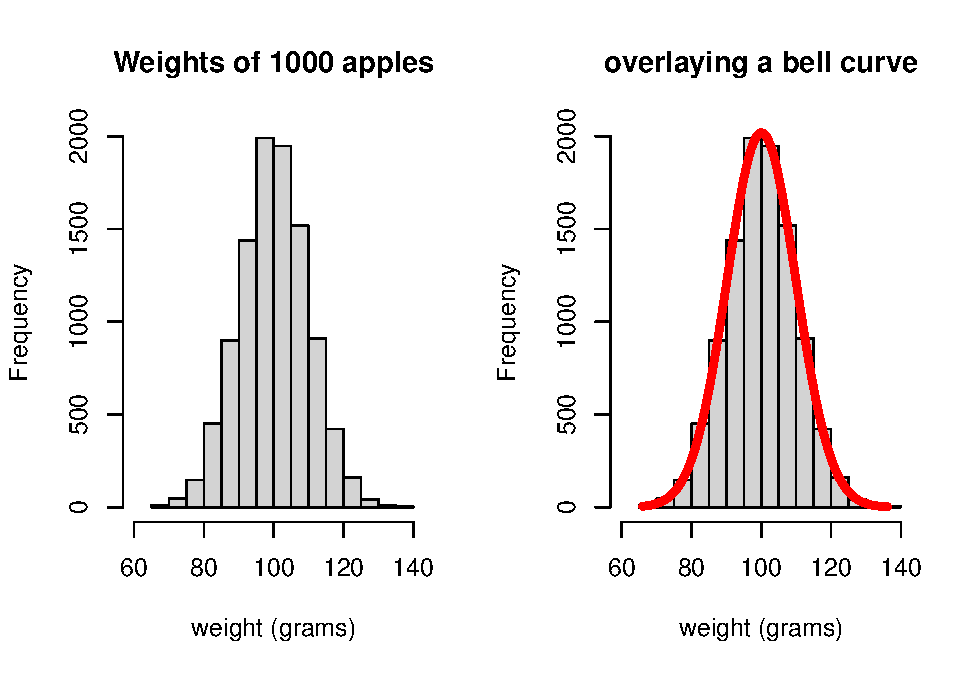
\includegraphics{6G4Z3008-notes_files/figure-latex/rnormhist-1.pdf}
\caption{\label{fig:rnormhist}A bell-shaped curve}
\end{figure}

\hypertarget{cauchy-density}{%
\section{Cauchy density}\label{cauchy-density}}

To study curves like the normal distribution it can be useful to consider what kinds of graphs could produce a curve with a single peak (unimodal) which are zero asymptotically.

Consider the curve

\[f(x) = \frac{1}{x^2+1}\]
Note \(f(0)=1\), and the square ensures it is everywhere positive. Notice the denominator cannot be zero, for \(x^2+1=0\) has no real roots.

When \(x\to \infty\), we divide by a larger and larger denominator so \(f(x)\to 0\). Similarly for \(x\to -\infty\).

People thought this curve looked like a witch's hat and is named after Italian Mathematician Maria Agnesi. The curve is called the `Witch of Agnesi'. Here is a graph of this curve:

\begin{figure}

{\centering 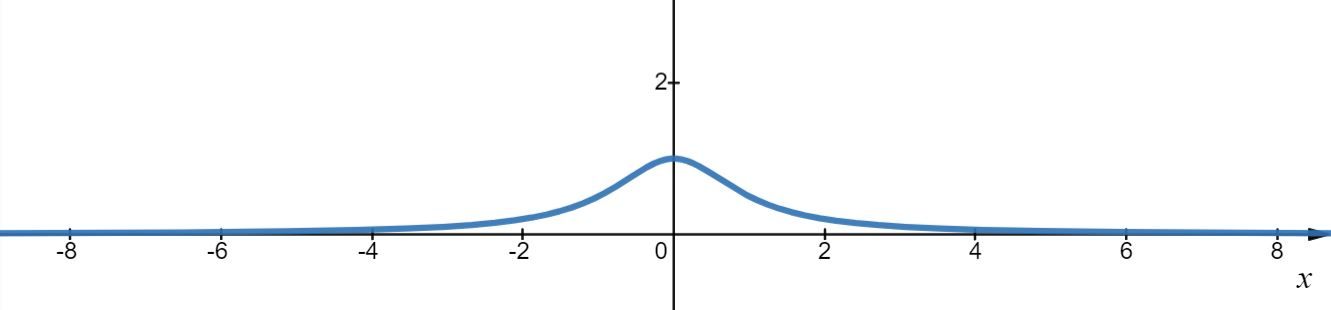
\includegraphics[width=0.75\linewidth]{./figures/cauchy} 

}

\caption{The Cauchy distribution}\label{fig:cauchy}
\end{figure}

However for this to be a density we need the integral to equal \(1\).

We can consider the integral

\[\int_{\mathbb{R}}\frac{1}{x^2+1} \ dx\]
You can use a trigonometric substitution here, for example \(x=\tan \theta\). Then

\[\frac{dx}{d\theta} = \sec^2\theta,\]
and \(1+x^2 = 1+\tan^2\theta = \sec^2 \theta\).

Then

\[\int_{\mathbb{R}}\frac{1}{x^2+1} \ dx = \int_{-\frac{\pi}{2}}^{\frac{\pi}{2}}1 \ d\theta \]

\[ = \left[\frac{\pi}{2} - \left(- \frac{\pi}{2}\right)\right] = \pi\]

The point of this example is that unexpectedly the number \(\pi\) crops up and we must divide by this \emph{normalising constant} so that the function

\[f(x) = \frac{1}{\pi(x^2+1)} ,\]
is a valid density function as it has integral \(1\).

\hypertarget{normal-density}{%
\section{Normal density}\label{normal-density}}

We will consider a function similar in shape to the above, namely

\[f(x) = e^{-\frac{1}{2}x^2} \]
It turns out that

\[\int _{-\infty}^{\infty} e^{-\frac{1}{2}x^2} \ dx = \sqrt{2\pi}\]
A Mathematical curiosity is that you can integrate \(e^{-\frac{1}{2}x^2}\) over the whole real line and get this result, but there exists no closed form (without integrals) antiderivative.

The upshot is that the integral involves \(\pi\) and so to make this a valid density we must have a factor involving \(1/{\sqrt{\pi}}.\) This should give you some intuition for the following definition.

\begin{definition}
A continuous random variable \(X\) is said to have a normal distribution with mean \(\mu\) and variance \(\sigma^2\), written \(X\sim \text{N}(\mu,\sigma^2)\) if it has the density function given by

\[ f(x) = \frac{1}{\sqrt{2\pi \sigma^2}}\text{exp}\left\{ -\frac{(x-\mu)^2}{2\sigma^2}\right\}, \]
where \(x, \mu\in \mathbb{R}\) and \(\sigma^2 > 0\).
\end{definition}

The density \(f(x)\) is a valid density, with the fraction \(\frac{1}{\sqrt{2\pi}\sigma}\) called the \emph{normalising constant} to ensure that the integral is \(1\) over the real line. The mean \(\text{E}(X)\) of this distribution is \(\mu\). The variance \(\text{Var}(X)\) is \(\sigma^2\). These three facts can be shown after studying \textbf{\emph{multi-variable calculus}} in second year.

The density of a normal distribution is a bell-shaped curve which is symmetric about the mean value \(\mu\). Most of the area under the curve is concentrated about the mean value with a relatively small amount at values a long way from \(\mu\). In general the density looks like the following picture, with a bell-shaped bump which tails off the zero at infinity either side. The curve is symmetrical about the line \(x=\mu\).

\begin{figure}

{\centering 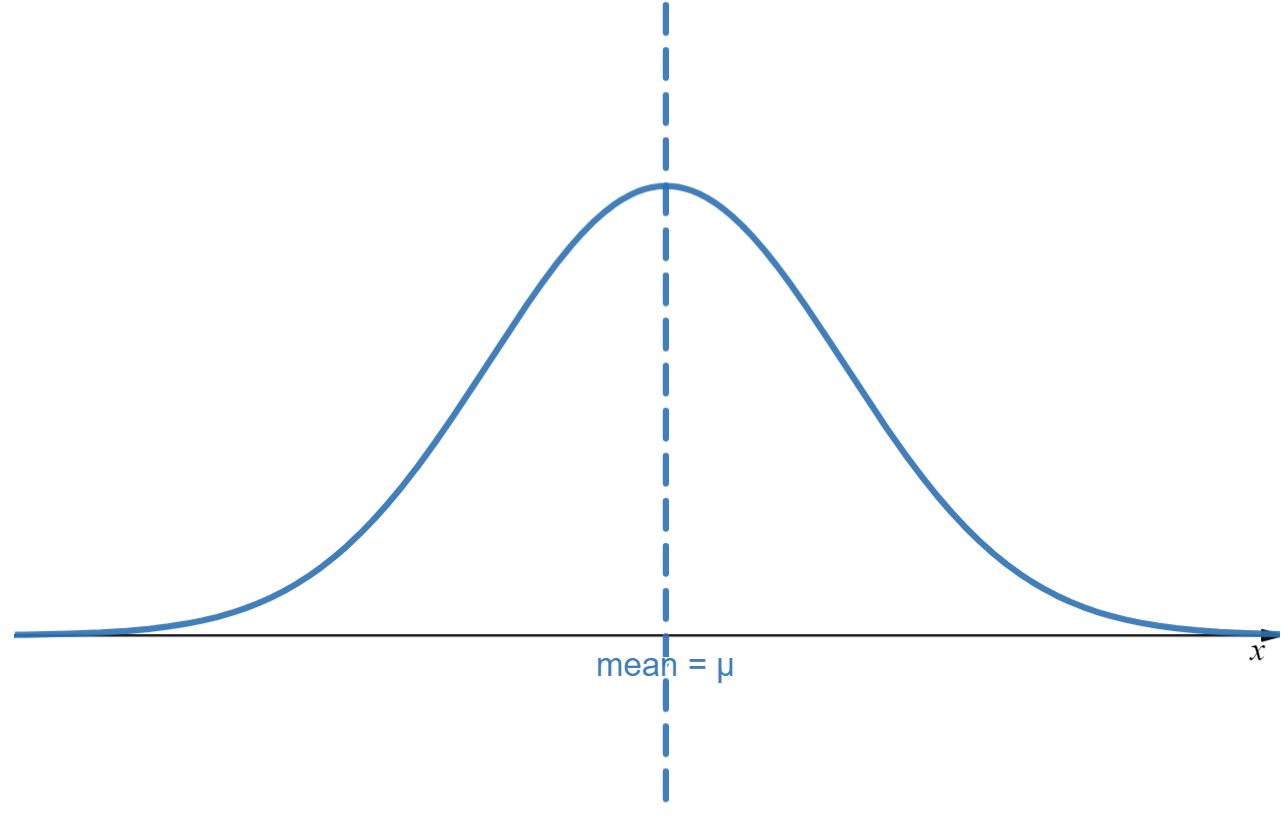
\includegraphics[width=0.75\linewidth]{./figures/norm1} 

}

\caption{a normal density curve is bell shaped}\label{fig:norm1}
\end{figure}

Changing the value of \(\mu\), will perform a translation along the \(x\) axis, and thereby the position of the centre of the curve.

\begin{figure}

{\centering 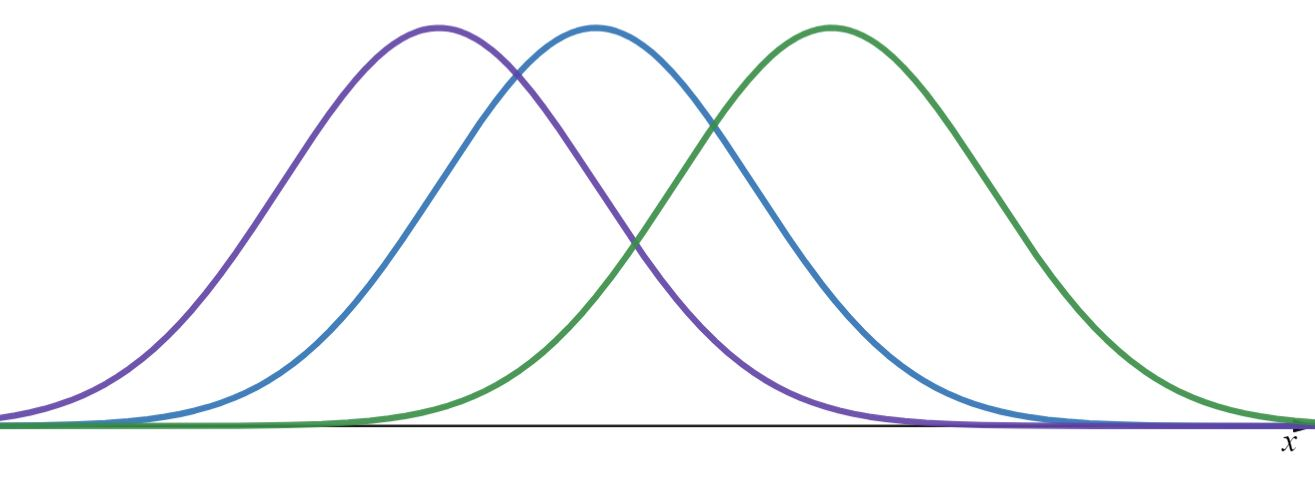
\includegraphics[width=0.75\linewidth]{./figures/norm2} 

}

\caption{three normal densities with the same standard deviation = 10, but means 90, 100 and 115}\label{fig:norm2}
\end{figure}

Changing the value of the standard deviation, or equivalently the variance, parameter determines how spread out the curve is about the mean. A smaller standard deviation results in a higher peak, as the model is less spread out and so is more mass around the mean value.

Conversely a larger standard deviation results in a lower peak, and more mass is spread out from the mean value towards the tails of the density.

We can view the

\begin{figure}

{\centering 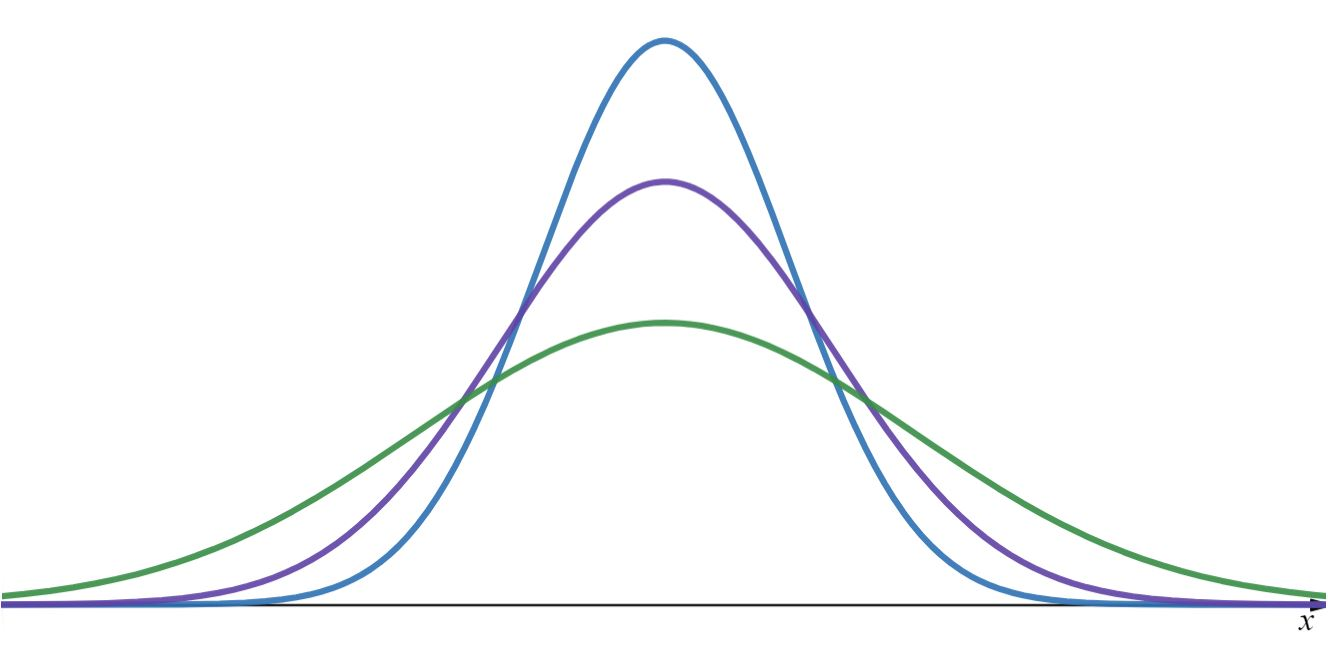
\includegraphics[width=0.75\linewidth]{./figures/norm3} 

}

\caption{three normal densities with the same mean, but standard deviations equal to 7.5, 10 and 15}\label{fig:norm3}
\end{figure}

One can access the normal density in R with the function \(\texttt{dnorm}()\), which we will see in labs.

\hypertarget{standard-normal}{%
\section{Standard normal}\label{standard-normal}}

\begin{definition}
The normal distribution with \(\mu=0\) and \(\sigma =1\) is called the standard normal distribution and is denoted by the letter \(Z\). Instead of \(f\) the density is denoted with the letter \(\phi\) and we have

\[\phi (z) = \frac{1}{\sqrt{2\pi}} \exp \left( -\frac{1}{2}z^2 \right) , z\in \mathbb{R}\]

The cumulative distribution function of the normal distribution is denoted with the capital \(\Phi(z) = \text{P}(Z\leq z)\).
\end{definition}

A graph of the density of the standard normal distribution \(Z\) is given below.

\begin{figure}

{\centering 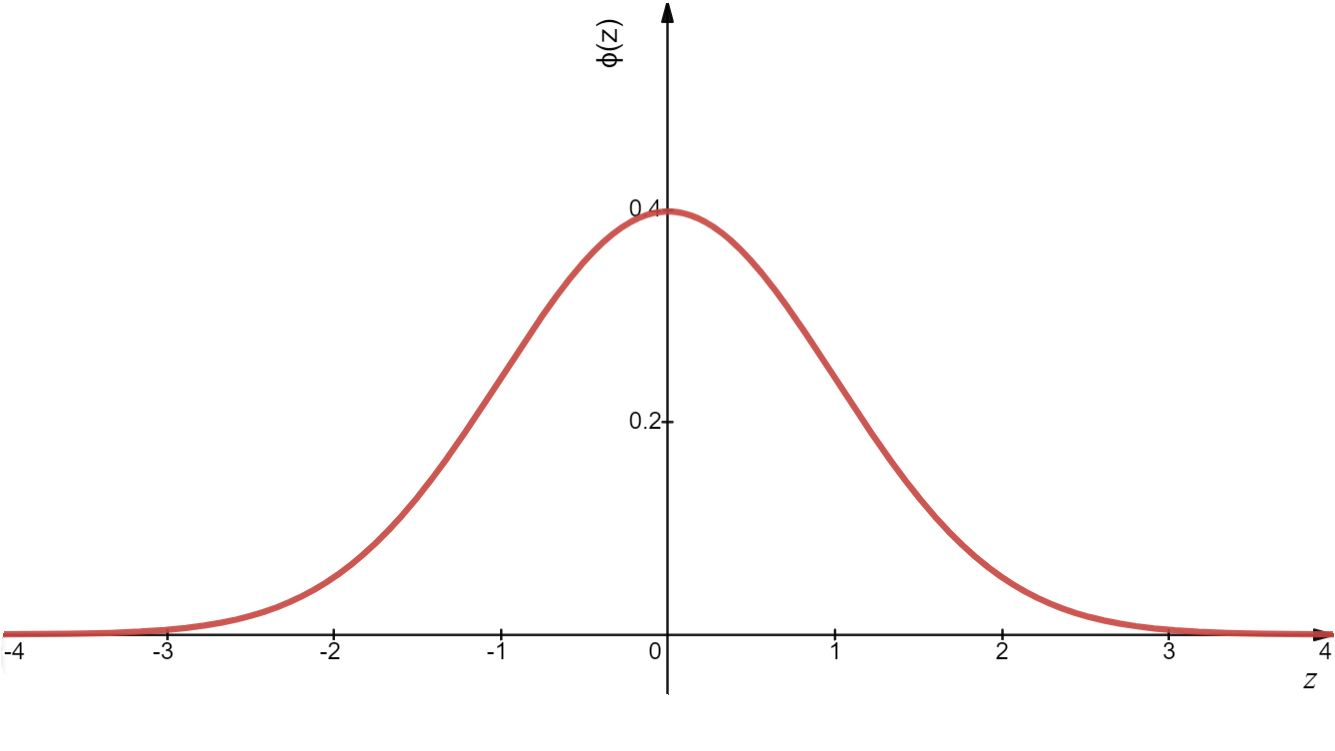
\includegraphics[width=0.75\linewidth]{./figures/znorm} 

}

\caption{the standard normal density}\label{fig:norm4}
\end{figure}

Notice that the majority of the area is between \(-3\) and \(3\). The distribution function of the standard normal is given in all statistical tables. We will see how problems involving any normal distribution can be recast in terms of the standard normal distribution.

\hypertarget{evaluating-the-standard-normal-distribution}{%
\section{Evaluating the standard normal distribution}\label{evaluating-the-standard-normal-distribution}}

The MMU tables give areas, i.e.~probabilities, in the \emph{tail} of the distribution for \(z>0\). Tables vary, some giving the left tail \(\text{P}(Z\leq z)\) (cumulative distribution \(\Phi\)), others give the upper tail \(\text{P}(Z\geq z)\), and if you are using tables you should read carefully the top-matter that describes the tabulation. The tables will only display the positive values of \(z\) in either format.

However, using tables we can find any area by observing:

\begin{enumerate}
\def\labelenumi{\arabic{enumi}.}
\item
  The area under the whole graph is 1. The law of complements applies so that \(\text{P}(Z\geq z)= 1-\text{P}(Z\leq z)\).
\item
  The graph is symmetric about \(0\). Lower tail areas with negative \(z\) value, are equal to the corresponding upper tail area with positive \(z\) value. In particular this implies that the areas above and below \(0\) are both \(0.5\).
\end{enumerate}

It is generally advised to draw a sketch of the density which shows the values required for the particular problem and the areas representing the probabilities.

\begin{example}

Use tables to find the following probabilities for a standard Normal random variable \(Z\).

\begin{enumerate}
\def\labelenumi{\arabic{enumi}.}
\item
  \(\text{P}(Z\geq 2.45)\)
\item
  \(\text{P}(Z\leq -2.45)\)
\item
  \(\text{P}(Z\leq 1.73)\)
\item
  \(\text{P}(Z\geq -0.5)\)
\item
  \(\text{P}(0.35\leq Z\leq 1.68)\)
\end{enumerate}

\end{example}

\emph{solutions}

\begin{enumerate}
\def\labelenumi{\arabic{enumi}.}
\item
  If the upper tail values are tabulated, we find this directly.
  \(\text{P}(Z\geq 2.45) = 0.0071\)
\item
  By symmetry we can argue that this is the same as the previous value.
  \(\text{P}(Z\geq 2.45) = 0.0071\)
\item
  Using complements \(\text{P}(Z\leq 1.73)= 1-\text{P}(Z\geq 1.73)\). From tables \(\text{P}(Z\geq 1.73)= 0.0418\), so \(\text{P}(Z\leq 1.73)= 1- 0.0418 = 0.9582\).
\item
  We have \(\text{P}(Z\geq -0.5) = 1 - \text{P}(Z\leq -0.5)\) by complements. Now also we have \(\text{P}(Z\leq -0.5) = \text{P}(Z\geq 0.5) = 0.3085\) by symmetry. Hence \[\text{P}(Z\geq -0.5) = 1 - 0.3085 = 0.6915 \]
\item
  We have \(\text{P}(0.35\leq Z\leq 1.68) = \text{P}(Z\geq 0.35)-\text{P}(Z\geq 1.68)\), looking up the latter two values gives \(0.3632 - 0.0465 = 0.3167.\)
\end{enumerate}

It is an important skill to be able to use statistical tables, and to familiarise yourself with their format. There may be other means of getting these numbers for particular distributions, for example using R or a calculator.

However later in the course some distributions will only appear in tables and you will be expected to use the tables in an exam.

\hypertarget{standardising}{%
\section{Standardising}\label{standardising}}

In the previous section we only considered the special case of a standard normal distribution (with mean \(0\) and variance \(1\)) for evaluating probabilities. We know that a normal distribution can be defined in general for any mean \(\mu\) and variance \(\sigma^2\). It is not possible to produce a table of values for every possible value of \(\mu\) and \(\sigma\). Fortunately it is also unnecessary.

\begin{theorem}
Suppose \(X\) follows a normal distribution with some mean and variance, so that \(X\sim \text{N}(\mu,\sigma^2)\), then subtracting the mean and dividing by the standard deviation results in a standard normal distrbution. That is,

\[\frac{X-\mu}{\sigma} \sim \text{N}(0,1) \]
Because of this result we write \(Z=\frac{X-\mu}{\sigma}\).
\end{theorem}

\emph{intuition}

\[\text{E}\left(\frac{X-\mu}{\sigma}\right)=\frac{1}{\sigma}\text{E}(X-\mu) \]
by linearity of the expectation, and,

\[ = \frac{1}{\sigma}(\text{E}(X) - \text{E}(\mu)) = \frac{1}{\sigma}(\mu-\mu)=0\]
as the expectation of a contant is just that constant.

For the variance,

\[ \text{Var} \left( \frac{X-\mu}{\sigma} \right) = \frac{1}{\sigma^2}\text{Var}(X-\mu)\]
By the the rule \(\text{Var}(aX)=a^2\text{Var}(X)\). Now the variance of a constant is zero so we have,

\[= \frac{1}{\sigma^2}\left( \text{Var}(X) - \text{Var}(\mu) \right) = \frac{1}{\sigma^2}\left( \sigma^2 - 0\right) = 1\]
Hence \(\frac{X-\mu}{\sigma}\) has the correct mean and variance. It remains to formally show it has the same density function as \(Z\), and so is normal.

An important consequence of the theorem which enables us to work out any probability is the following corollary.

\begin{corollary}
Suppose \(X\) follows a normal distribution with some mean and variance, so that \(X\sim \text{N}(\mu,\sigma^2)\) then

\[\text{P}(a\leq X \leq b) = \Phi\left(\frac{b-\mu}{\sigma}\right) - \Phi\left(\frac{a-\mu}{\sigma}\right)\]
\end{corollary}

\emph{proof}
\[\text{P}(a\leq X \leq b) = \text{P}\left(\frac{a-\mu}{\sigma} \leq \frac{X-\mu}{\sigma}  \leq  \frac{b-\mu}{\sigma}\right) = \text{P}\left(\frac{a-\mu}{\sigma} \leq Z  \leq  \frac{b-\mu}{\sigma}\right) \]
Where the last equality is by the theorem. Now recall \(\Phi\) is the CDF of \(Z\), so the result follows.

This formula has a very simple geometric interpretation. Recall that we can represent probabilities for continuous random variables as the area, between specified limits, under the distribution curve. This theorem just says that the area under \emph{any} Normal curve between limits \(a\) and \(b\) is always the same as the area under the standard Normal
curve between the \emph{transformed} limits \(\frac{a-\mu}{\sigma}\) and \(\frac{b-\mu}{\sigma}\).

\begin{example}

Suppose that the weight of a particular grade of apples is Normally distributed with mean 100g and standard deviation 8g. Let \(X\) denote the weight of a randomly selected apple, i.e.~\(X\sim\text{N}(100,{8^2})\), find:

\begin{enumerate}
\def\labelenumi{\arabic{enumi}.}
\item
  \(P(X>115)\)
\item
  \(P(X< 80)\)
\item
  \(P(105<X<112)\)
\item
  \(P(95<X<112)\)
\end{enumerate}

\end{example}

\emph{solution}

\begin{enumerate}
\def\labelenumi{\arabic{enumi}.}
\tightlist
\item
  \[P(X>115)  =  P\left(Z>\frac{115-100}{8}\right)
          =  P(Z>1.88)\]
\end{enumerate}

This quantity can be found directly from tables, i.e.
\(P(Z>1.88)=0.0301\).

\begin{enumerate}
\def\labelenumi{\arabic{enumi}.}
\setcounter{enumi}{1}
\tightlist
\item
  \[P(X<80)  =  P\left(Z<\frac{80-100}{8}\right)
          =  P(Z<-2.5)
          =  P(Z>2.5)\]
\end{enumerate}

From tables, \(P(Z>2.5)=0.0062\)

\begin{enumerate}
\def\labelenumi{\arabic{enumi}.}
\setcounter{enumi}{2}
\item
\end{enumerate}

\[P(105<X<112)  =  P\left(\frac{105-100}{8}<Z<\frac{112-100}{8}\right)\]

\[= P(0.63<Z<1.5)\]
\[=P(Z>0.63)-P(Z>1.5)\]
\[= 0.2643-0.0668=0.1975\]
4.
There are several ways in which this problem could be approached - a sketch or diagram will help. We have,

\[P(95<X<112) =  P\left(\frac{95-100}{8}<Z<\frac{112-100}{8}\right)
          =  P(-0.63<Z<1.5)\]

But,

\[P(Z<-0.63)+P(-0.63<Z<1.5)+P(Z>1.5)=1\]

\begin{itemize}
\tightlist
\item
  the three areas comprise the whole distribution. We also have,
  \[P(Z<-0.63)=P(Z>0.63)\]
  by symmetry, so that
\end{itemize}

\[P(-0.63<Z<1.5) =  1-P(Z>0.63)-P(Z>1.5)\]

\[=  1-0.2643-0.0668=0.6689\]

\hypertarget{inverse-cdf}{%
\section{Inverse CDF}\label{inverse-cdf}}

We saw how to solve problems which involved finding the probability that a Normally distributed
random variable lay in a certain range. The solution to this problem consisted of two steps:

\begin{itemize}
\tightlist
\item
  standardising the the value of the original variable to get a standard Normal variable.
\item
  using tables of the standard Normal distribution to find the required probability, recognising that the process of
  standardisation preserves areas, i.e.~probabilities.
\end{itemize}

We may think of the process as follows:
\[ \mbox{Original Value,
}X\stackrel{\frac{x-\mu}{\sigma}}{\longrightarrow} Z
\longrightarrow \mbox{Probability ?}
\]
The inverse problem, as the name suggests, is simply the same
process but applied backwards. We start out with a probability and seek to find
the value of the random variable corresponding to that probability. Thus, since

\[Z  =  \frac{X-\mu}{\sigma} \]
\[\Rightarrow \sigma Z = X-\mu \]
\[\Rightarrow X  =  \mu+\sigma Z\]

The inverse problem can be thought of as working through
the following process,
\[ \mbox{Original Value,
}X\mbox{? }\stackrel{\sigma Z+\mu}{\longleftarrow} Z
\longleftarrow \mbox{Probability}
\]
As before a simple sketch graph of the problem is invaluable.

\begin{example}
The weights of eggs laid by a particular breed of hens are
Normally distributed with mean \(50\)g and standard deviation \(5\)g. An
egg producer wants to classify eggs so that the heaviest \(10\)\% are
classified as large and the lightest \(30\)\% classified as small. The
remaining \(60\)\% are classified as medium. What weights should be
used to distinguish the three classes?
\end{example}

If we let the random variable \(X\) denote the weight of an egg,
we need to find the values of \(x_1\) and \(x_2\) indicated in the
following diagram,

\begin{figure}

{\centering 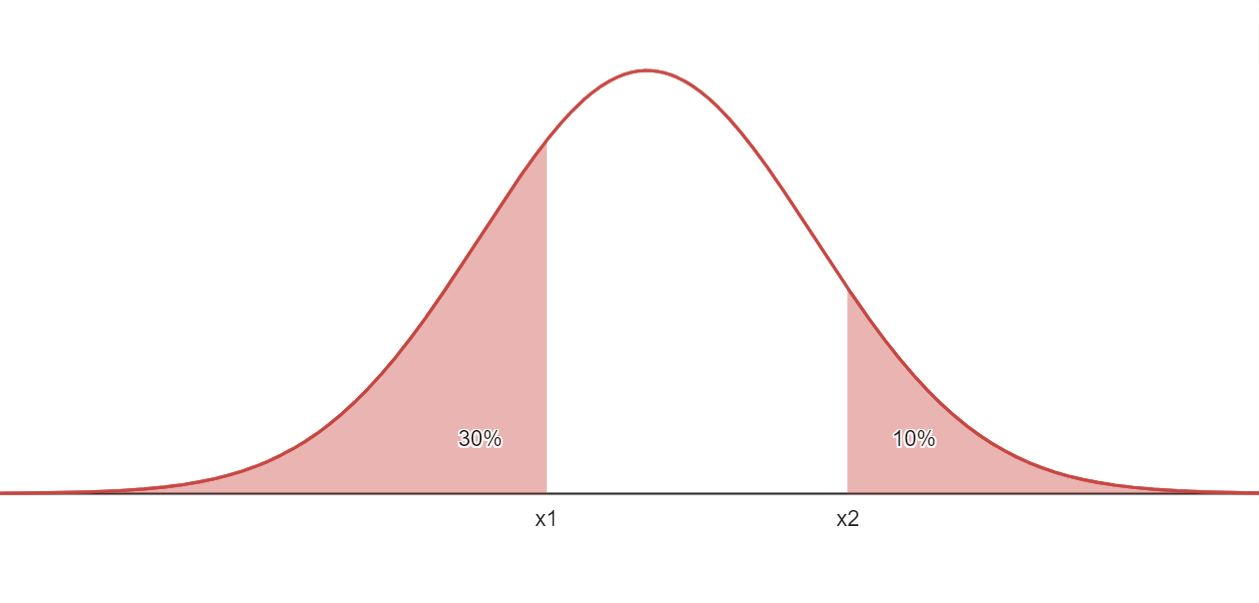
\includegraphics[width=0.75\linewidth]{./figures/eggs} 

}

\caption{proportions of eggs by weight}\label{fig:eggs}
\end{figure}

Common sense, and our knowledge of the Normal distribution, tells us that the value of \(x_1\) is a \emph{little} below the mean value of \(50\)g and the value of \(x_2\) somewhat higher than the mean value of \(50\)g. In fact, we can usually make a reasonably accurate guess if we use the result that virtually all the curve (99.7\%) is contained within the limits \(\pm\) 3 standard deviations either side of the mean. In case, virtually all the eggs will lie in the range \([50-3\times 5,50+3\times5]\)=\([35,65]\)g.

In order to solve the problem, we have to find the values of a standard normal variable corresponding to the same probabilities indicated on the diagram above.

The \(z\) value exceeded with a probability 0.1 is found to be 1.2816, i.e.~\[P(Z\geq 1.2816)=0.1\].

At the other end of the distribution we find the probability a \(Z\) value is less than 0.3 is -0.5244, i.e.~
\[P(Z\leq -0.5244)=0.3\].

Note that this last value was found using the symmetry of the distribution. You should check that these are the \(z\) values you would have obtained if you had been working the other way round.

Note that, if the required probability is not in the \emph{inverse} tables, you have to use the main table backwards. To do this, look for the required probability (or as close as you can get to it) in the body of the table, and then read off the corresponding \(z\)-value.

For example, scanning through the body of the table, we find that a probability of 0.1003 corresponds to a \(z\) value of 1.28 and a probability of 0.0985 corresponds to a z-value of 1.29. Clearly, the actual value corresponding to a probability of 0.10 (which we know is 1.2816) is somewhere between 1.28 and 1.29. In practice, a good estimate can be found using interpolation.

\begin{figure}

{\centering 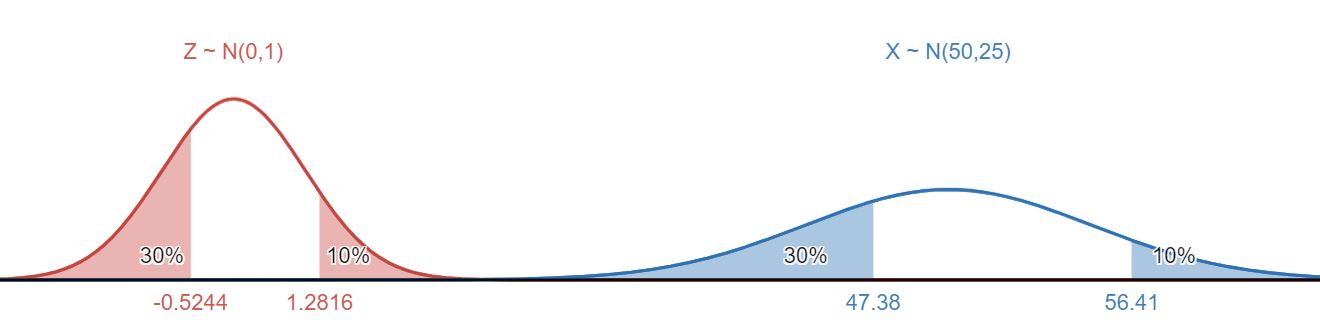
\includegraphics[width=0.75\linewidth]{./figures/inverseeggs} 

}

\caption{Standardised values of the egg weight distribution give the same area in the tails}\label{fig:inveggs}
\end{figure}

The final stage of the problem is to apply the inverse transformation to get the appropriate values on the original
scale. Recall, the inverse transformation is, \(X=\sigma Z+\mu\).
Thus we, have,

\begin{enumerate}
\def\labelenumi{\alph{enumi})}
\item
  The weight which will be exceeded by the largest 10\% of eggs is given
  by, \(X = 5\times 1.2816+50 = 56.41\)g.
\item
  The weight which the smallest 30\% of eggs will lie below is
  given by, \(X = 5\times -0.5244+50 = 47.38\)g
\end{enumerate}

\begin{example}

A vending machine discharges hot chocolate. The volume of liquid the machine discharges may be modelled by a normal distribution. With probability \(5\%\), the volume discharged is greater than \(475\)ml. While the probability of the volume being less than \(460\)ml is one percent.

\begin{enumerate}
\def\labelenumi{\alph{enumi})}
\item
  Sketch a picture to show this information
\item
  Find \(\mu\) and \(\sigma\).
\end{enumerate}

\end{example}

\hypertarget{sampling-total}{%
\section{Sampling Total}\label{sampling-total}}

\subsection{Distribution of Sample Total}

Suppose we have an independent random sample of size \(n\) from a Normal distribution,
e.g.~\(X_1,\ldots,X_n\sim \text{N}(\mu,\sigma^2)\).

Define the random variable \(T=\sum_{i=1}^n X_i\), then,
\[ T \sim \text{N}(n\mu,n\sigma^2). \]

That is, the \emph{sampling distribution} of the total, \(T\), is also Normally distributed with \(\text{E}(T)=n\mu\) and \(\text{Var}(T)=n\sigma^2\).

\begin{example}[apples revisited]

Earlier we assumed that the weight of
individual apples sold by a supermarket were Normally distributed
with mean 100g and standard deviation 8g, i.e.~if the random variable \(X\)
represents the weight then \(X \sim \text{N}(100,{8^2})\).

Let the random variable \(T\) denote the total weight of a carton of 4 apples. Find the probability that the total weight of a carton is,

\begin{enumerate}
\def\labelenumi{\alph{enumi})}
\item
  more than 450g
\item
  between 375g and 425g
\end{enumerate}

\end{example}

\emph{solution}

Here \(n=4\), \(\mu=100\) and \(\sigma=8\) so that, the total weight,
\[ T\sim \text{N}({4\times 100},{4\times 8^2})\sim \text{N}({400},{16^2}) \]
We answer the problem by converting to a standard Normal as before,

\begin{enumerate}
\def\labelenumi{\alph{enumi})}
\tightlist
\item
  We have,
\end{enumerate}

\[P(T>450)  =  P\left(Z>\frac{450-400}{16}\right)\]
\[=  P(Z>3.13)\]
\[ =  0.0009\]

\begin{enumerate}
\def\labelenumi{\alph{enumi})}
\setcounter{enumi}{1}
\tightlist
\item
  We have,
\end{enumerate}

\[P(375<T<425)  =  P\left(\frac{375-400}{16}<Z<\frac{425-400}{16}\right) \]
\[=  P(-1.56<Z<1.56)=1-2\times P(Z>1.56)\]
\[=  1-2\times 0.0594=0.8812\]

\hypertarget{sampling-distribution-of-the-mean}{%
\section{Sampling distribution of the mean}\label{sampling-distribution-of-the-mean}}

All the problems considered so far have supposed that a single
measurement is randomly drawn from some population in which the
possible values of the measurement follow a Normal distribution.
We now consider what happens if we,

\begin{itemize}
\item
  Take a random sample of size \(n\) from a population whose
  values follow a Normal distribution. We will denote the random sample of
  values by \(X_1,X_2,\ldots,X_n\). For example, we might
  randomly select \(n=10\) people and measure their height.
\item
  Calculate the \textbf{\emph{mean}} value of the sample, i.e.~
  \[\bar{X}=\frac{X_1+X_2+\ldots+X_n}{n}=\frac{1}{n}\sum_i X_i\]
\item
  Calculate the \textbf{\emph{total}} value of the sample, i.e.~
  \[T = X_1+X_2+\ldots+X_n =\sum_i X_i\]
\end{itemize}

Now, since each member of the sample is a random variable, the sample mean must also be a random variable.

\begin{example}
The heights of two randomly selected MMU students are \(X_1\) and \(X_2\). Given a particular sample, i.e.~two actual students say \(x_1=170\)cm and \(x_2=158\)cm, we can calculate their mean \(\bar{x}=164\)cm. However until we pick the sample, the quantity \((X_1+X_2)/2\) is random. So we can treat this mean as a random variable and denote it with a capital letter \(\bar{X}\).
\end{example}

\begin{definition}
A \textbf{\emph{statistic}} is a random variable whose particular values can be calculated from a particular sample. For example the statistic \(\bar{X}\) is calculated as \(\frac{X_1+X_2+\ldots+X_n}{n}\).
\end{definition}

Given a random variable one can always ask `what is its distribution?'.

The following result can only be quoted.

\begin{theorem}
Suppose that random variables \(X_1,X_2,\ldots,X_n\) each follow a
Normal distribution with mean \(\mu\) and variance \(\sigma^2\), i.e.
\(X_i\sim \text{N}({\mu},{\sigma^2})\). Then, for the sample mean \(\bar{X}\), we
have the \emph{sampling distribution} of that statistic is
\[\bar{X}\sim \text{N}(\mu,\frac{\sigma^2}{n})\]
\end{theorem}

\emph{proof}
This proof is beyond the scope of the course, however we can check the mean and variance are as described.

What this result says is that the sample mean has the same theoretical population mean, \(\mu\), as any single value drawn from the population, but that its variance is reduced by a factor \(n\). Given our knowledge of the role of the variance in the Normal distribution, the result suggests that sample mean ought to lie closer to the true population mean \(\mu\) as the sample size increases.

\begin{example}
Suppose I take \(10\) samples of bamboo shoots and measure their lengths. The length of these particular bamboo shoots are normally distributed with mean \(74\)mm and standard deviation \(5\)mm.

\begin{longtable}[]{@{}ccc@{}}
\toprule
Sample & Shoot lengths(mm) & Sample mean\tabularnewline
\midrule
\endhead
1 & 76,73,75,73,74,74,74,74,74,77 & 74.4\tabularnewline
2 & 74,72,75,76,73,71,73,80,75,75 & 74.4\tabularnewline
3 & 68,72,78,74,75,74,69,77,77,72 & 73.6\tabularnewline
4 & 72,76,76,77,70,77,72,74,77,76 & 74.7\tabularnewline
5 & 78,72,70,74,76,72,73,71,74,74 & 73.4\tabularnewline
6 & 75,79,75,74,75,74,71,73,75,73 & 74.4\tabularnewline
7 & 75,70,73,75,70,72,72,71,76,73 & 72.7\tabularnewline
8 & 74,76,74,75,74,76,75,75,73,73 & 74.5\tabularnewline
9 & 78,74,73,75,74,73,72,76,73,76 & 74.4\tabularnewline
10 & 74,71,72,71,79,78,69,77,73,71 & 73.5\tabularnewline
\bottomrule
\end{longtable}

The range in values of the shoot lengths is from \(68\) to \(80\). The values of the statistic \(\bar{X}\) vary noticably less, are close to the original mean value of \(74\)mm.
\end{example}

Now we have two variances \(\sigma^2\) and \(\sigma^2/n\) or equivalently standard deviations \(\sigma\) and \(\sigma / \sqrt{n}\) we need to be clear which one we are talking about.

\begin{definition}
The quantity \(\sigma/\sqrt{n}\) is called the \textbf{\emph{standard error of the
mean}}. This is the standard deviation of \(\bar{X}\) - the sampling distribution of the mean. It is essentially the same as the standard deviation for a single observation but reflects the fact that the variance of
the mean depends on the sample size \(n\).
\end{definition}

As \(n\) gets larger and larger, the distribution of the sample mean
gets more and more concentrated around the value of the population
mean \(\mu\).In practice, this suggests that, if the true
population mean were unknown, the sample mean ought to be a good
estimate of its value.

\begin{example}

Apple weights (revisited)
Recall we assumed that the weight of individual apples sold by a supermarket were Normally distributed
with mean 100g and standard deviation 8g, i.e.~if the random variable \(X\)
represents the weight then \(X \sim \text{N}({100},{8^2})\).

The supermarket also sells apples in cartons of four. What is the
probability that the mean weight of the apples in a randomly
selected carton is,

\begin{enumerate}
\def\labelenumi{\alph{enumi})}
\tightlist
\item
  more than 105g
\item
  less than 98g
\item
  between 98 and 102g
\end{enumerate}

\end{example}

\emph{solution}
Here \(n=4\), \(\mu=100\) and \(\sigma=8\). If we denote the mean weight
of the apples in a carton by \(\bar{X}\), then,
\[ \bar{X} \sim \text{N}({100},8^2/4) \sim \text{N}(100,16)\]

In this case the standard error of the mean is
\(8/\sqrt{4}=\sqrt{16}=4\). Having calculated the standard error, we
answer such problems in the same way as before by converting the
problem to one involving the standard Normal distribution.

\begin{enumerate}
\def\labelenumi{\alph{enumi})}
\item
  \[P(\bar{X} \geq 105)  =  P\left ( Z \geq \dfrac{105-100}{4}\right) \]
  \[=  P(Z\geq 1.25)\]
  \[=  0.1056\]
\item
\end{enumerate}

\[P(\bar{X} \leq 98)  =  P\left ( Z \leq \dfrac{98-100}{4}\right)\]

\[=  P(Z\leq -0.5)=P(Z\geq 0.5)\]
\[= 0.3085\]

\begin{enumerate}
\def\labelenumi{\alph{enumi})}
\setcounter{enumi}{2}
\tightlist
\item
  \[P(98\leq \bar{X} \leq 102)  = P\left (\dfrac{98-100}{4} \leq Z \leq \dfrac{102-100}{4}\right)\]
\end{enumerate}

\[=  P(-0.5\leq Z\leq 0.5)=1-2\times P(Z\geq 0.5)\]
\[=  0.3830\]

\hypertarget{exercises-week-6}{%
\section{Exercises week 6}\label{exercises-week-6}}

\begin{exercise}
Suppose the lifetime of an electrical component follows
a uniform distribution on the range \([0,2000]\) hours.

\begin{enumerate}
\def\labelenumi{\alph{enumi})}
\item
  Draw a sketch of the distribution.
\item
  Find the probability that the lifetime will be,
\end{enumerate}

\begin{enumerate}
\def\labelenumi{(\roman{enumi})}
\tightlist
\item
  at least 1000 hours
\item
  less than 250 hours
\item
  between 500 and 1500 hours
\end{enumerate}

(draw a sketch of the distribution and the area under the
distribution representing the probability)
\end{exercise}

\begin{exercise}

The time taken (in minutes) to serve a customer in a fast food
restaurant is a continuous random variable, \(X\), with probability
distribution,
\[ f(x) = \left \{\begin{array}{ll}
  \dfrac{x}{2}& 0\leq x \leq 2 \\
  0 & \mbox{otherwise}
\end{array} \right .
\]

\begin{itemize}
\tightlist
\item
  Sketch the density.
\item
  Show that the area under the distribution is one.
\item
  You only need to use the areas of triangles to answer these
  questions. Find the probability that the time taken to serve a
  customer will be,
\end{itemize}

\begin{enumerate}
\def\labelenumi{\roman{enumi}.}
\tightlist
\item
  less than one minute
\item
  more than one minute
\item
  more than 30 seconds
\item
  between 30 seconds and 1 minute.
\end{enumerate}

\end{exercise}

\begin{exercise}

Use standard Normal tables to find the following
probabilities, (draw a sketch diagram in each case)

\begin{enumerate}
\def\labelenumi{\roman{enumi}.}
\item
  \(P(Z>1.7)\)
\item
  \(P(Z>2.35)\)
\item
  \(P(Z<-0.92)\)
\item
  \(P(Z<-2.33)\)
\item
  \(P(0.78<Z<2.56)\)
\item
  \(P(-1.99<Z<-0.34)\)
\item
  \(P(-1.67<Z<2.58)\)
\end{enumerate}

\end{exercise}

\begin{exercise}

The lifetime of a certain brand of lightbulb is Normally distributed with
mean 2000 hours and standard deviation 75 hours. Find the probability that a
randomly selected bulb will have lifetime,

\begin{enumerate}
\def\labelenumi{\alph{enumi}.}
\item
  greater than 2100 hours
\item
  greater than 2200 hours
\item
  less than 2050 hours
\item
  less than 1950 hours
\item
  between 1950 and 2100 hours
\item
  between 2050 and 2200 hours
\item
  between 1900 and 1950 hours
\end{enumerate}

\end{exercise}

\begin{exercise}

Bags of sugar packed by a machine have a mean weight of 2kg and a
standard deviation of 0.02kg. Find the probability that the weight of a
bag will be

\begin{enumerate}
\def\labelenumi{\roman{enumi}.}
\item
  greater than 2.05kg
\item
  less than 1.96kg
\item
  between 1.95 and 2.05kg
\item
  less than 2.03kg
\item
  between 1.95 and 1.98 kg
\item
  between 2.01 and 2.05 kg
\end{enumerate}

\end{exercise}

\begin{exercise}

A type of laboratory mouse has weight which is Normally distributed with mean
30g and standard deviation 2.5g. Find the probability that the weight of a randomly
selected mouse is,

\begin{enumerate}
\def\labelenumi{\alph{enumi}.}
\item
  at least 33g
\item
  less than 33.5g
\item
  more than 29g
\item
  less than 28g
\item
  between 27g and 33g
\item
  between 31g and 33.5g
\end{enumerate}

\end{exercise}

\begin{exercise}
Eggs are classified as standard, if they weigh less than
46.0g, medium if they weigh between 46.0g and 56.0g, or large if
they weigh over 56.0g. Suppose the eggs laid by a particular
breed of hen have weight which is Normally distributed with mean
50.0g and standard deviation 5.0g. What percentage of eggs laid by
these hens falls into the three classes?
\end{exercise}

\begin{exercise}
A manufactured item requires a fuse which can be supplied by one
of two suppliers. Supplier 1's fuses have a lifetime which is Normally distributed
with mean 1000 hours and standard deviation 30 hours. Supplier 2's fuses have a
lifetime which is Normally distributed with mean 990 hours and standard deviation
10 hours. Your product specification requires that fuses should last at least 980
hours. Which of the two suppliers would you choose and why.
\end{exercise}

\begin{exercise}

Marks in a statistics examination are Normally
distributed with mean 50 and standard deviation 10. What is the
probability that

\begin{enumerate}
\def\labelenumi{\roman{enumi})}
\item
  the mean mark of a group of 5 students will be above 60?
\item
  the mean mark of a group of 20 students will be between 44
  and 48?
\end{enumerate}

\end{exercise}

\begin{exercise}
A ski-lift is designed with a load limit of 18,000lbs and claims a
capacity of 100 people. If the weight of people using the lift is Normally
distributed with mean 175lbs and standard deviation 30lbs, what is the
probability that a group of 100 randomly selected people will exceed the load
limit of the lift? Would you be willing to use the lift?
\end{exercise}

\begin{exercise}

Lengths of bicycle chain links are Normally distributed with mean
0.5cm and standard deviation 0.04cm. The finished chains must be between 49
and 50cm long.

\begin{enumerate}
\def\labelenumi{\alph{enumi})}
\item
  If the chains are made of 100 links, what proportion meets the
  standard?
\item
  If chains are made instead of 99 links what proportion meets the
  standard?
\item
  Using 99 links, to what value must the standard deviation be reduced in
  order to have the following percentages meet the standard?
\item
  90\%\\
\end{enumerate}

\begin{enumerate}
\def\labelenumi{\roman{enumi})}
\setcounter{enumi}{1}
\tightlist
\item
  95\%\\
\item
  99\%\\
\end{enumerate}

\end{exercise}

\begin{exercise}
Bags of sugar packed by a machine have a mean weight of 2kg and a standard
deviation of 0.02kg. What weights will

\begin{enumerate}
\def\labelenumi{\alph{enumi})}
\item
  be exceeded by 15\% of bags
\item
  be exceeded by 90\% of bags
\item
  20\% of bags contain less than
\item
  90\% of bags be between
\item
  A multipack contains 5 bags of sugar. What is the probability that
\item
  All the bags contain less than 1.992 kg
\end{enumerate}

\begin{enumerate}
\def\labelenumi{\roman{enumi})}
\setcounter{enumi}{1}
\tightlist
\item
  Exactly four bags contain less than 1.992kg
\end{enumerate}

(Hint: Consider using the normal distribution and then the Binomial
with the appropriate probability.)
\end{exercise}

\begin{exercise}
The weight of a child can be modelled as normally distributed with mean \(30\)kg and standard deviation \(5\)kg.

A fairground ride has a total carrying capacity of \(2.8\) metric tons (thousand kilograms).

\(k\) children are admitted to the ride and their total weight \(X_1+X_2+ \ldots + X_k\).

What is the maximum number of children that could be admitted to the ride, to ensure that the total weight is within the carrying capacity with probability \(99\%\)?
\end{exercise}

\begin{exercise}

The masses of penguins on an island are found to be normally distributed with mean \(\mu\) and standard deviation \(\sigma\). Given that \(10\%\) of the penguins have mass less than \(18\)kg and \(5\%\) have mass greater than \(30\)kg,

\begin{enumerate}
\def\labelenumi{\alph{enumi})}
\item
  Sketch a diagram to represent this information
\item
  Find \(\mu\) and \(\sigma\).
\end{enumerate}

\end{exercise}

\hypertarget{sampling-and-confidence-intervals}{%
\chapter{Sampling and confidence intervals}\label{sampling-and-confidence-intervals}}

This week we begin the Statistical applications of the theory we have learned so far.

We will learn the basis of (Frequentist) statistical inference. We will construct and interpret confidence intervals for a mean and a proportion. We will then introduce hypothesis testing.

If Mathematics is a deductive process, Statistics is an inferential one. Given imperfect information (usually data), we make (sensible) inferences about models of the real world.

Most modelling situations involve estimating the value of a population parameter or characteristic, and one of the main tasks in Statistics is to estimate the values of the parameters from sample data.

\begin{example}
Suppose we are interested in the average height of an adult man in the UK. The \textbf{\emph{population}} of interest is then all UK adult men (approximately \(33\) million). A \emph{model} for the height of men may be a normal distribution:

\[X\sim \text{N}(\mu,\sigma^2),\]

where \(\mu\) and \(\sigma^2\) are the \textbf{\emph{population parameters}} of the distribution.

Why might it not be possible to measure the height of every UK man? Instead we take a smaller number of men to measure, say \(100\) or \(1000\). This is called a \textbf{\emph{sample}}.

From the sample we can calculate the sample mean \(\bar{x}\) and the sample standard deviation \(s\).
\end{example}

Population parameters like \(\mu\) are in practice unknowable with certainty. Typically in statistics we may specifically want to

\begin{itemize}
\item
  Estimate the value of \(\mu\).
\item
  Determine a range or interval of plausible values for \(\mu\).
\item
  Decide whether a particular value of \(\mu\) appears to be reasonable.
\end{itemize}

We distinguish between real world, or population parameters, and sample statistics in the following table:

\begin{longtable}[]{@{}lll@{}}
\toprule
Characteristic & Population parameter & Sample statistic / estimator\tabularnewline
\midrule
\endhead
Mean & \(\mu\) & \(\bar{x}\)\tabularnewline
Standard deviation & \(\sigma\) & \(s\)\tabularnewline
Proportion & \(\pi\) & \(\hat{p}\),\(p\)\tabularnewline
\bottomrule
\end{longtable}

It is intuitively obvious that we can use the sample mean to estimate the true value of the population mean. However we must recognise that when drawing a random sample, from a normal distribution in this case, any statistic calculated from the sample will also have a probability distribution.

Recall \textbf{\emph{Theorem 6.2}} from last week. The sampling distribution of the mean \(\bar{X}\) is normally distributed with the same mean but with variance divided by a factor given by the sample size \(n\). That is

\[\overline{X} \sim \text{N} (\mu, \sigma^2/{n})\]

With larger values of \(n\) we can compare the proportion of the density about the mean.

\begin{example}

Suppose we assume the percentage of glucose in bars of toffee is normally distributed with mean \(20\%\) and standard deviation \(2\%\). Find the probability that:

\begin{enumerate}
\def\labelenumi{\alph{enumi})}
\item
  One bar of toffee selected at random has glucose level between \(19.5\%\) and \(20.5\%\).
\item
  The mean percentage glucose in \(20\) randomly selected toffee bars is between \(19.5\%\) and \(20.5\%\).
\item
  The mean percentage glucose in \(100\) randomly selected toffee bars is between \(19.5\%\) and \(20.5\%\).
\end{enumerate}

\end{example}

\emph{solution}

\begin{enumerate}
\def\labelenumi{\alph{enumi})}
\tightlist
\item
  \[\text{P}(19.5<X<20.5)= \text{P}\left(\frac{19.5-20}{2}<Z<\frac{20.5-20}{2}\right)\]
\end{enumerate}

\[= \text{P}(-0.25<Z<0.25)=1-2\times\text{P}(Z>0.25)\]

\[=1-2\times 0.4013=0.20\]

\begin{enumerate}
\def\labelenumi{\alph{enumi})}
\setcounter{enumi}{1}
\tightlist
\item
  \[\text{P}(19.5<\overline{X}<20.5)= \text{P}\left(\frac{19.5-20}{\sqrt{2^2 / 20}}<Z<\frac{20.5-20}{\sqrt{2^2 / 20}}\right)\]
\end{enumerate}

\[= \text{P}(-1.12<Z<1.12)=1-2\times\text{P}(Z>1.12)\]

\[=1-2\times 0.1314=0.74 \approx 75\%\]

\begin{enumerate}
\def\labelenumi{\alph{enumi})}
\setcounter{enumi}{2}
\tightlist
\item
  \[\text{P}(19.5<\overline{X}<20.5)= \text{P}\left(\frac{19.5-20}{\sqrt{2^2 / 100}}<Z<\frac{20.5-20}{\sqrt{2^2 / 100}}\right)\]
\end{enumerate}

\[= \text{P}(-2.5<Z<2.5)=1-2\times\text{P}(Z>2.5)\]

\[=1-2\times 0.0062=0.99\ldots \approx 99\%\]

We can summarise this example with the following table:

\begin{longtable}[]{@{}cc@{}}
\toprule
Sample size \(n\) & \(\text{P}(19.5 <\overline{X} < 20.5)\)\tabularnewline
\midrule
\endhead
1 & \(20\)\tabularnewline
20 & \(75\%\)\tabularnewline
100 & \(99\%\)\tabularnewline
\bottomrule
\end{longtable}

We can use the sampling distribution in various ways to make inferences about the true population mean glucose content. For example, in a samle of \(100\) toffee bars, and assuming the true mean is \(\mu=20\%\), a value of \(\bar{x}\) outside the range \(19.5 - 20.5\%\) would appear very unusual.

\hypertarget{confidence-intervals}{%
\section{Confidence Intervals}\label{confidence-intervals}}

This specifies a range of plausible values for the parameter of interest.

Recall we can find a particular value of \(Z\sim \text{N}(0,1)\) within which the distribution has a specified probability - using the inverse CDF of the normal distribution.

\begin{example}
Calculate the \(z\)-value containing the middle \(95\%\) of density. In other words find \(z\) such that \(\text{P}(|Z|\leq z)=0.95\).

\emph{solution}

Recall \(|x|<1\) means \(-1<x<1\).

The inequality \(|Z|\leq z\) means \(-z\leq Z\leq z\).

\[\text{P}(-z\leq Z \leq z)=0.95\]
\[\iff  \text{P}(Z\geq z) = P(Z\leq -z) =0.025\]
From tables:

\[\Phi^{-1}(0.025) = -1.96\]
Or alternatively \[\Phi^{-1}(0.975) = 1.96\]

So \(z=1.96\), and \(\text{P}(|Z|<1.96) =0.95\)
\end{example}

Note that \(95\% = 100(1-0.05)\%\). The \(z\) value we calculated corresponded to \(\alpha / 2\).

\begin{definition}
A confidence interval for the population mean \(\mu\) of level \(100(1-\alpha)\%\) is given by the following expression.

\[\left( \bar{x}-z_{\frac{\alpha}{2}}\frac{\sigma}{\sqrt{n}},\bar{x}+z_{\frac{\alpha}{2}}\frac{\sigma}{\sqrt{n}} \right)\]
\end{definition}

The confidence interval is derived from standardisation of the sampling distribution of the mean. That is,

\[\overline{X} \sim \text{N} (\mu, \sigma^2/{n}),\]
implies

\[Z = \frac{\overline{X} - \mu}{\sigma / \sqrt{n}} \sim \text{N}(0,1).\]

\[\text{P}\left( |Z| <z_{\frac{1}{2}\alpha} \right) = 1-\alpha\]

Now by standardisation replace \(Z\) with the expression involving \(\overline{X}\).

\[\text{P}\left( \left|\frac{\overline{X} - \mu}{\sigma / \sqrt{n}} \right| <z_{\frac{1}{2}\alpha} \right) = 1-\alpha\]
The denominator is positive so this is equivalent to:
\[\text{P}\left( |\overline{X} - \mu| <z_{\frac{1}{2}\alpha} \frac{\sigma}{\sqrt{n}}  \right) = 1-\alpha\]

\[\text{P}\left( |\mu - \overline{X} | <z_{\frac{1}{2}\alpha} \frac{\sigma}{\sqrt{n}}  \right) = 1-\alpha\]

\[\text{P}\left(z_{\frac{1}{2}\alpha} \frac{\sigma}{\sqrt{n}} < \mu - \overline{X} <z_{\frac{1}{2}\alpha} \frac{\sigma}{\sqrt{n}}  \right) =1-\alpha\]
\[\text{P}\left( \overline{X}+ z_{\frac{1}{2}\alpha} \frac{\sigma}{\sqrt{n}} < \mu <\overline{X} + z_{\frac{1}{2}\alpha} \frac{\sigma}{\sqrt{n}}  \right) =1-\alpha\]

\begin{example}
The milligrams of fat in a sample of hotdogs were measured as
\[25.2, \ 21.3,\ 22.8,\ 17.0,\ 29.8,\ 21.0,\ 25.5,\ 16.0,\ 20.9, \ 19.5\]
Supposing that the fat content is normally distributed, that this is a random sample of hotdogs, and the population standard deviation \(\sigma = 5\), calculate a \(90\%\) confidence interval for the mean fat content \(\mu\).
\end{example}

\emph{solution}

With \(90\%\) centrally, we must have \(5\%\) in either tail. One can look up the \(z\) value as \(z_{0.95}= 1.6449\).

In R we could get this value with the quantile command \(\texttt{qnorm(0.95,mean=0,sd=1)}\).

Then,
\[\bar{x} \ \pm \ z\frac{\sigma}{\sqrt{n}} = 21.9 \ \pm 1.6449\times\frac{5}{\sqrt{10}}\]

\[=[19.3 , 24.5] \text{   (to 3 s.f.)}\]

Warning - there are many incorrect interpretations of confidence intervals, and it is contentious how meaningful such an interval is.

Note that while \(\mu\) is unknown, it is a constant rather than a random quantity. We cannot say ``with \(95\%\) chance \(\mu\) will lie inside the interval'', because there is no chance associated to a constant quantity.

The random part of the interval comes from \(\overline{X}\), so rather we must say that with repeated samples, and in the long run, approximately \(95\%\) of intervals will contain \(\mu\).

Another misconception is to say that if there were 100 such intervals, exactly 95 would contain the interval, but this is a general error about the interpretation of probability.

Below is some R code to simulate this process.

\begin{Shaded}
\begin{Highlighting}[]
\KeywordTok{library}\NormalTok{(plotrix)}
\end{Highlighting}
\end{Shaded}

\begin{verbatim}
## Warning: package 'plotrix' was built under R version 4.0.5
\end{verbatim}

\begin{Shaded}
\begin{Highlighting}[]
\NormalTok{z<-}\KeywordTok{qnorm}\NormalTok{(}\FloatTok{0.975}\NormalTok{,}\DecValTok{0}\NormalTok{,}\DecValTok{1}\NormalTok{) }\CommentTok{# this is the z-value }
\NormalTok{sigma <-}\StringTok{ }\DecValTok{5}
\NormalTok{x<-}\StringTok{ }\DecValTok{1}\OperatorTok{:}\DecValTok{100}

\KeywordTok{set.seed}\NormalTok{(}\DecValTok{1234}\NormalTok{) }\CommentTok{#ensures the code is reproducible}

\CommentTok{#100 samples of 10 hotdogs each}
\NormalTok{hotdogs <-}\StringTok{ }\KeywordTok{replicate}\NormalTok{(}\DecValTok{100}\NormalTok{, }\KeywordTok{rnorm}\NormalTok{(}\DecValTok{10}\NormalTok{,}\DataTypeTok{mean=}\DecValTok{20}\NormalTok{,}\DataTypeTok{sd=}\DecValTok{5}\NormalTok{))}

\CommentTok{#Calculate the mean of each sample}
\NormalTok{xbar <-}\StringTok{ }\KeywordTok{vector}\NormalTok{(}\DataTypeTok{length =} \DecValTok{100}\NormalTok{)}
\ControlFlowTok{for}\NormalTok{ (i }\ControlFlowTok{in} \DecValTok{1}\OperatorTok{:}\DecValTok{100}\NormalTok{)\{}
\NormalTok{xbar[i] <-}\StringTok{ }\KeywordTok{mean}\NormalTok{(hotdogs[}\KeywordTok{seq}\NormalTok{(}\DecValTok{10}\OperatorTok{*}\NormalTok{(i}\DecValTok{-1}\NormalTok{),}\DecValTok{10}\OperatorTok{*}\NormalTok{i,}\DecValTok{1}\NormalTok{)])}
\NormalTok{\}}

\CommentTok{#lower end of interval L}
\NormalTok{L <-}\StringTok{ }\NormalTok{xbar }\OperatorTok{-}\StringTok{ }\NormalTok{z}\OperatorTok{*}\NormalTok{sigma}\OperatorTok{/}\KeywordTok{sqrt}\NormalTok{(}\DecValTok{10}\NormalTok{)}

\CommentTok{#upper end of interval U}
\NormalTok{U <-}\StringTok{ }\NormalTok{xbar }\OperatorTok{+}\StringTok{ }\NormalTok{z}\OperatorTok{*}\NormalTok{sigma}\OperatorTok{/}\KeywordTok{sqrt}\NormalTok{(}\DecValTok{10}\NormalTok{)}

\KeywordTok{plotCI}\NormalTok{(x, xbar, }\DataTypeTok{ui=}\NormalTok{U, }\DataTypeTok{li=}\NormalTok{L,}\DataTypeTok{ylab=}\StringTok{"hotdog fat content"}\NormalTok{)}
\KeywordTok{abline}\NormalTok{(}\DataTypeTok{a=}\DecValTok{20}\NormalTok{, }\DataTypeTok{b=}\DecValTok{0}\NormalTok{,}\DataTypeTok{col=}\StringTok{"red"}\NormalTok{, }\DataTypeTok{lwd=}\DecValTok{3}\NormalTok{, }\DataTypeTok{lty=}\DecValTok{2}\NormalTok{)}
\end{Highlighting}
\end{Shaded}

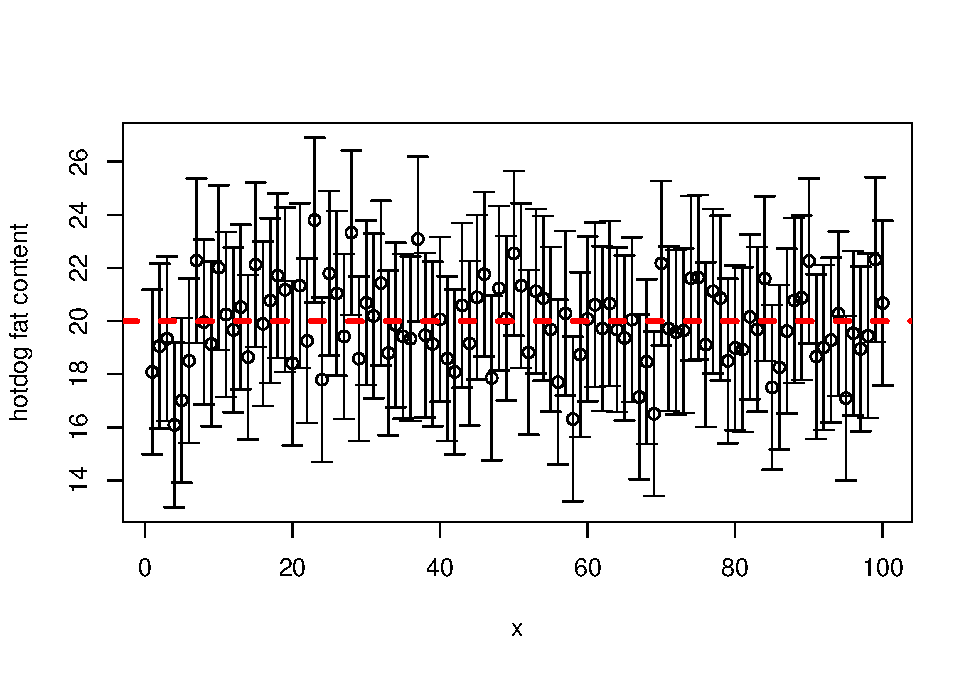
\includegraphics[width=0.75\linewidth]{6G4Z3008-notes_files/figure-latex/ci_sim-1}

In this example it turns out that \(5\%\) of intervals did not contain the mean. However setting a different seed shows this is not fixed, just a long term probability.

In many scientific studies all the data is pooled in a single sample, and one calculates a single confidence interval. There is no way of knowing if the interval contains the mean. What `confidence' do we really have here?

If \(\bar{x}\) is a single-valued or \emph{point estimate}, the C.I. is just by convention just an \emph{interval estimate}.

\hypertarget{unknown-variance}{%
\section{Unknown variance}\label{unknown-variance}}

What do we do if we do not know \(\sigma\)? Well we have to estimate it.

\hypertarget{estimating-the-variance}{%
\subsection{Estimating the variance}\label{estimating-the-variance}}

Recall we estimate the population parameters such as \(\mu\) with statistics like \(\bar{X}\).

We can ask what the expected value of a statistic is

\[\text{E}(\overline{X})= \text{E}\left( \frac{1}{n}\sum_{i=1}^{n}X_i \right)\]

\[=\frac{1}{n}\sum_{i=1}^{n}\text{E}(X_i) = \frac{1}{n}\sum_{i=1}^{n}\mu =\frac{1}{n}n\mu=\mu\]

We can see that \(\text{E}(\bar{X})=\mu\).

\begin{definition}
When a statistic is used to estimate a parameter, if the expectation of the estimator is equal to the parameter, then the statistic is called \textbf{\emph{unbiased}}.

Hence \(\bar{X}\) is an unbiased estimator for \(\mu\).
\end{definition}

It turns out that the obvious choice to estimate \(\sigma^2\) is not unbiased.

\[\text{E}\left( \frac{1}{n}\sum_{i=1}^{n}(X_i-\bar{X})^2 \right) = \frac{1}{n}\text{E}\left( \sum_{i=1}^n (X_i^2-2\bar{X} X_i +\bar{X}^2)\right) \]

\[=\frac{1}{n}\text{E}\left( \sum_{i=1}^n X_i^2 -2\bar{X}\sum_{i=1}^n{X_i} +\sum_{i=1}^n \bar{X}^2 \right) \]

\[=\frac{1}{n}\text{E}\left( \sum_{i=1}^n X_i^2 -2n\bar{X}^2 +n \bar{X}^2 \right) =\frac{1}{n}\text{E}\left( \sum_{i=1}^n X_i^2 -n\bar{X}^2  \right)  \]

\[=\frac{1}{n}\left( \sum_{i=1}^n \text{E}(X_i^2) -n\text{E}(\bar{X}^2)  \right) \]
Using the identity \(\text{Var}(X)= \text{E}(X^2)=\text{E}(X)^2\) gives:

\[=\frac{1}{n}\left( \sum_{i=1}^n [\text{Var}(X_i)+\text{E}(X_i)^2] -n[\text{Var}(\bar{X})+\text{E}(\bar{X})^2]  \right) \]
And now we have \(\text{Var}(X_i) = \sigma^2\), \(\text{E}(X_i)^2 = \mu^2\), \(\text{E}(\bar{X}) = \mu\), and \(\text{Var}(\bar{X})=\frac{\sigma^2}{n}\). Putting this together gives.

\[=\frac{1}{n}\left( \sum_{i=1}^n [\sigma^2+\mu^2] -n\left[\frac{\sigma^2}{n}+\mu^2\right]  \right) =\frac{1}{n}\left( n\sigma^2+n\mu^2-n\left[\frac{\sigma^2}{n}+\mu^2\right]\right)\]

Altogether

\[\text{E}\left( \frac{1}{n}\sum_{i=1}^{n}(X_i-\bar{X})^2 \right) = \frac{(n-1)\sigma^2}{n} \]

To make a statistic that is an unbiased estimator for \(\sigma^2\), we could rescale by multiplying by \(n\) and dividing by \((n-1)\).

If the variance \(\sigma\) is unknown, an unbiased estimate of \(\sigma\) is

\[s^2 = \frac{1}{n-1}\sum_{i=1}^n (x_i-\bar{x})^2\]

This has the property that \(\text{E}(S^2) = \sigma^2\).

It may in practice be easier to compute:

\[s^2= \frac{1}{n-1}\left(\sum_{i=1}^n x_i^2 - n\bar{x}^2\right) = \frac{1}{n-1}\left(\sum x_i^2 - \frac{(\sum x_i)^2}{n}\right).\]
Check which appears in the formula booklet.

\hypertarget{the-t-distribution}{%
\subsection{The t distribution}\label{the-t-distribution}}

When we do not know the population variance \(\sigma^2\), we have more uncertainty. The more data we have the less uncertainty we have, but for small samples we need to account for this and use a distribution with more mass in the tails.

To deal with this we use the quantiles of the \(t\)-distribution instead of the quantiles of the \(Z\sim \text{N}(0,1)\). Below is a picture of a \(t\)-distribution,

\begin{figure}

{\centering 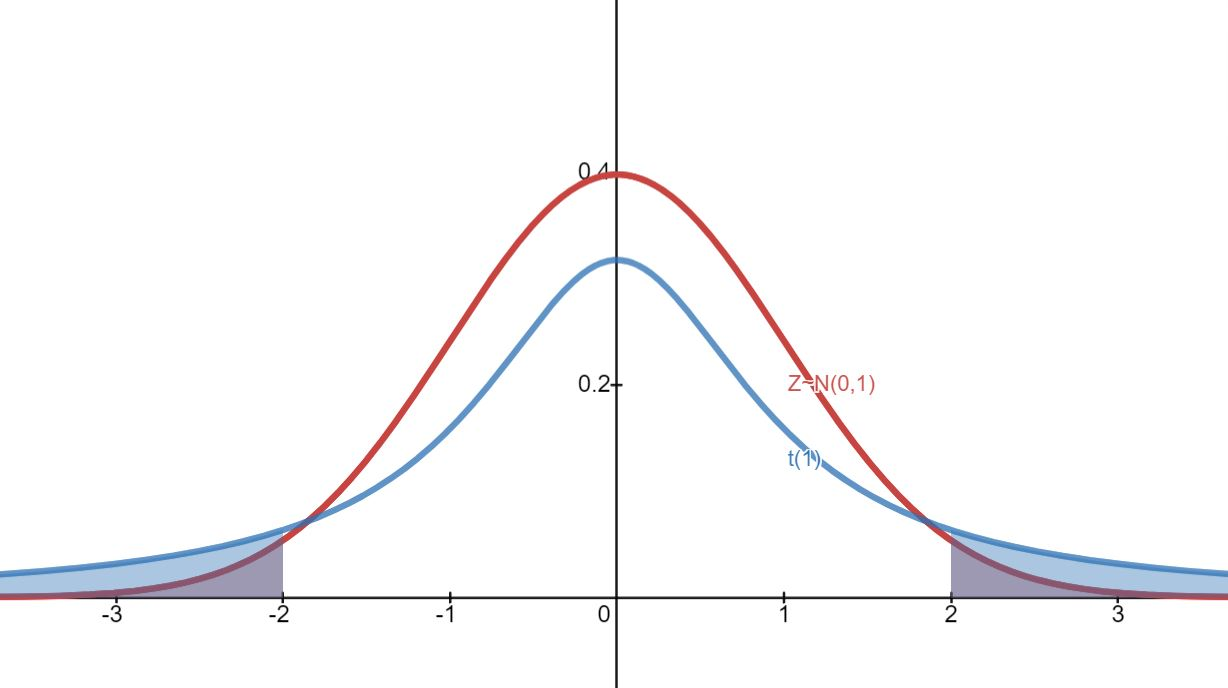
\includegraphics[width=0.75\linewidth]{./figures/tdist} 

}

\caption{fat tails of the t-distribution}\label{fig:t1}
\end{figure}

The \(t\)-distribution has a number of degrees of freedom to account for the decreased uncertainty in the tails with more data. As the number of degrees of freedom increases we can see the distribution approaches the standard normal density.

\begin{figure}

{\centering 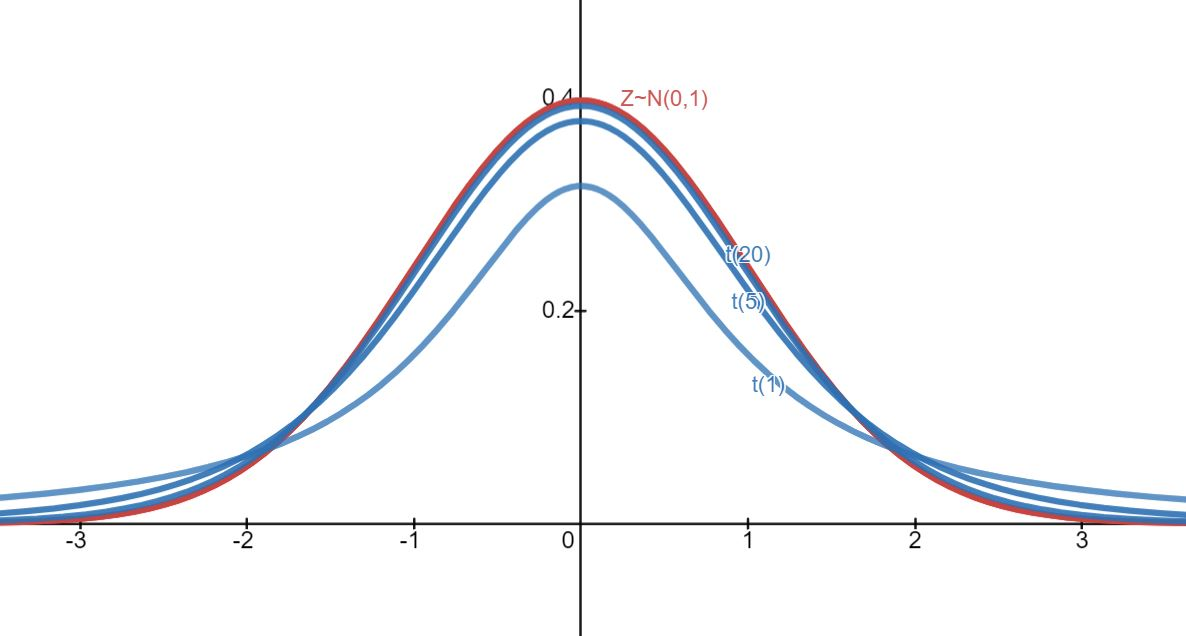
\includegraphics[width=0.75\linewidth]{./figures/df} 

}

\caption{t distributions with 1, 5 and 20 degrees of freedom}\label{fig:t2}
\end{figure}

\begin{definition}
For the \(t\)-distribution, the number of \textbf{\emph{degrees of freedom}} \(\nu\) is one less than the number of data points.

\[\nu = n-1\]
\end{definition}

\begin{definition}
Given a random sample of size \(n\) from a normally distributed population with unknown population variance a \(100(1-\alpha)\%\) confidence interval for the population mean \(\mu\) is given by

\[\left( \bar{x} - t_{n-1,\alpha /2} \frac{s}{\sqrt{n}}, \bar{x} + t_{n-1,\alpha /2} \frac{s}{\sqrt{n}}\right)\]
The quantiles of the \(t\)-distribution need to be obtained from the table in the formula booklet, or from the R function \(\texttt{qt()}\).
\end{definition}

\begin{example}

A sample of \(6\) trout taken from a fish farm were caught and their lengths in centimetres were measured. the lengths of the fish were as follows:

\[ 26.8, \ 26.0, \ 25.8, \ 25.5, \ 24.3, \ 24.6 \]

Assuming the lengths of the trout are normally distributed:

\begin{itemize}
\item
  Calculate unbiased estimates for the mean and variance.
\item
  Find a \(90\%\) confidence interval for the mean length of trout in the fish farm.
\end{itemize}

\end{example}

\emph{solution}
Using a calculator gives \(\bar{x}=25.5\) and \(s^2 = 0.8560\).

The \(90\%\) confidence limits for \(\bar{x}\) are:

\[\bar{x} \pm t_{5,5\%}\frac{s}{\sqrt{n}} = 25.5 \pm 2.015\times \frac{0.9252}{\sqrt{6}}\]

\[=(24.7,26.3)\]

\begin{example}[exam-style]

The masses in grams of ten packets of biscuits of a particular brand were weighed. The results are summarised by a computerised weighing machine as:

\[\sum x_i = 3978.8 \ , \ \sum x_i^2 = 1583098.3 \]

\begin{enumerate}
\def\labelenumi{\alph{enumi})}
\item
  What assumptions and requirements are necessary to produce a
  confidence interval for the mean weight of a packet of biscuits? Explain these in context.
\item
  Calculate unbiased estimates for the mean and variance.
\item
  Calculate a \(95\%\) confidence interval.
\item
  The weight on the packet says \(400\)g, does the data support this labelling?
\end{enumerate}

\end{example}

\emph{solution}

\begin{enumerate}
\def\labelenumi{\alph{enumi})}
\item
  The sample is assumed to be random. The weights are assumed to follow a normal distribution.
\item
  \[\bar{x} = 3978.8/10 = 397.88\text{g}\]
  \[s^2 = \frac{1}{10-1}\left(1583098.3-\frac{3978.8^2}{10}\right) =1.484\text{g}\]
\item
  The required interval is:
\end{enumerate}

\[\bar{x} \pm t_{9}(2.5\%)\frac{s}{\sqrt{n}} = 397.88 \pm 2.2622\times \frac{\sqrt{1.484}}{\sqrt{10}}\]
\[(397.0,398.8 ) \]

\begin{enumerate}
\def\labelenumi{\alph{enumi})}
\setcounter{enumi}{3}
\tightlist
\item
  As \(400\) lies outside the interval, this sample does not support the labelling.
\end{enumerate}

\hypertarget{required-sample-sizes}{%
\section{Required sample sizes}\label{required-sample-sizes}}

Note that the width of the confidence interval is determined by the required level of confidence and the sample size as long as we know or can estimate the standard deviation. We can use this to decide in advance how many observations are needed to estimate the mean with of a given degree of precision.

\begin{example}[Ikea]
From time to time a firm manufacturing pre-packed furniture needs to check the mean distance between pairs of holes drilled by a machine in pieces of chipboard to ensure that no change has occurred. It is known from experience that the standard deviation of the distance is \(0.43\)mm. The first intends to take a random sample of size \(n\), and to calculate a \(99\%\) confidence interval for the mean of the population. The width of this interval must be no more than \(0.60\)mm. Calculate the minimum value of \(n\).
\end{example}

\emph{solution}

The width is the difference between the end points of the interval, and so is twice the term that is added (and subtracted) from \(\bar{x}\) in the formula.

\[2z\frac{\sigma}{\sqrt{n}} <0.6\]
\[2\times 2.576\times \frac{0.43}{\sqrt{n}}<0.6\]
\[2\times 2.576\times {0.43}<0.6\sqrt{n}\]
\[\frac{2\times 2.576\times {0.43}}{0.6}<\sqrt{n}\]
\[\sqrt{n} > 3.69\ldots \]
\[n > 13.6\ldots \]
The smallest value of \(n\) is therefore \(14\).

\hypertarget{interval-for-a-population-variance}{%
\section{Interval for a population variance}\label{interval-for-a-population-variance}}

We have shown earlier that the sampling distribution of the sample variance has expectation \(\sigma^2\). That is, the random variable \(S^2\) given by:

\[S^2 = \frac{1}{n-1}\sum_{i=1}^n(X_i-\overline{X})^2 ,\]

is such that,

\[\text{E}(S^2) = \sigma^2\]
But as yet we do not know the distribution of \(S^2\).

We introduce the relevant distributions, prove a proposition and derive use this to derive a confidence interval for the variance.

\begin{definition}
A random variable \(Y\) is said to have a \textbf{\emph{chi-squared distribution}} with one degree of freedom, written \(Y\sim\chi^2(1)\) if it has density function:

\[f_Y(y) = \frac{1}{\sqrt{2\pi y}}e^{-y/2} \]
\end{definition}

\begin{proposition}
The square of a standard normal distribution \(Z^2\) follows a \(\chi^2(1)\) distribution. That is, if \(Z\sim N(0,1)\) then \(Z^2\sim \chi^2(1)\)
\end{proposition}

\emph{proof}

Recall the density and distribution functions of the standard normal are written in greek letters \(f_Z = \phi\) and \(F_Z = \Phi\). We will also need to remember from last week that \(\phi\) takes the form

\[\phi(z) =  \frac{1}{\sqrt{2\pi}} \exp \left( -\frac{1}{2}z^2 \right)\]

Consider the distribution function of \(Y=Z^2\).
\[ F_Y(z) = \text{P}(Z^2<z)\]
\[= \text{P}\left(-\sqrt{z}<Z<\sqrt{z}\right)\]
\[=\int_{-\sqrt{z}}^{\sqrt{z}}\phi(x) \ dx \]

\[=\int_{-\infty}^{\sqrt{z}}\phi(x) \ dx - \int_{\infty}^{-\sqrt{z}}\phi(x) \ dx\]
\[=\Phi(\sqrt{z})- \Phi(-\sqrt{z})\]
\[=\Phi(\sqrt{z})-(1-\Phi(\sqrt{z})), \text{ by symmetry}\]

\[=2\Phi(\sqrt{z})-1. \]

So \(F_Y(z) = 2\Phi(\sqrt{z})-1\). We can find the density by differentiating,

\[f_Y (z)= \frac{d}{dz}F_Y(z)\]
\[=\frac{d}{dz}\left[2\Phi(\sqrt{z})-1\right] \]

\[=2\Phi'(\sqrt{z})\times\frac{1}{2}z^{-\frac{1}{2}} , \text{by the chain rule}\]
\[=\Phi'(\sqrt{z})\times\frac{1}{\sqrt{z}}\]
But differentiating a distribution gives you the density, that is \(\Phi' = \phi\). Hence

\[=\phi(\sqrt{z})\times\frac{1}{\sqrt{z}}\]
\[=\frac{1}{\sqrt{2\pi}} \exp \left( -\frac{1}{2}(\sqrt{z})^2 \right) \times \frac{1}{\sqrt{z}}\]
\[=\frac{1}{2\pi z} e^{-z/2}. \]
But this is the density function of \(\chi^2(1)\), and if two random variables have the same density they must be equal, so we must have
\[Z^2 = \chi^2(1).\]
With this result it will not be hard to believe the following

\begin{proposition}
If \(Z_1 ,Z_2, \ldots, Z_k\) are independent standard normal random variables then a sum of squares these random variables is a chi-squared distribution with \(k\) degrees of freedom.

\[Z_1^2+Z_2^2+\ldots+ Z_k^2 \sim \chi^2(k) \]
\end{proposition}

proof: omitted.

\begin{theorem}
We can scale the sampling distribution of the sample variance to be a chi-squared distribution on \(n-1\) degrees of freedom.

\[\frac{(n-1)S^2}{\sigma^2} \sim\chi^2_{n-1}\]
\end{theorem}

\emph{proof}

\[S^2 =\frac{1}{n-1}\sum_{i=1}^n(X_i-\overline{X})^2 \]

\[(n-1)S^2 =\sum_{i=1}^n(X_i-\overline{X})^2 \]
\[\frac{(n-1)S^2}{\sigma^2} =\frac{1}{\sigma^2}\sum_{i=1}^n(X_i-\overline{X})^2 \]
\begin{equation}
\frac{(n-1)S^2}{\sigma^2} =\sum_{i=1}^n\left(\frac{X_i-\overline{X}}{\sigma}\right)^2
\label{eq:var}
\end{equation}
If \(\bar{X}\) were \(\mu\) we could view the RHS as a sum of squares of standardised variables. Let \(Q\) be the expression we wanted it to be

\[Q = \sum_{i=1}^n\left(\frac{X_i-\mu}{\sigma}\right)^2 \]

Then \(Q\sim \chi^2(n)\). Now we can manipulate

\[Q=\sum_{i=1}^n\left(\frac{(X_i- \bar{X}) + (\bar{X}-\mu)}{\sigma}\right)^2\]
Splitting this up gives:
\[=\sum_{i=1}^n\left(\frac{X_i - \bar{X}}{\sigma}\right)^2+2\left(\frac{\bar{X}-\mu}{\sigma}\right)\sum_{i=1}^n \left(\frac{X_i-\bar{X}}{\sigma}\right) + \sum_{i=1}^n\left(\frac{\bar{X} - \mu}{\sigma}\right)^2\]

\[=\underbrace{\sum_{i=1}^n\left(\frac{X_i - \bar{X}}{\sigma}\right)^2}_{(7.1)}+2\left(\frac{\bar{X}-\mu}{\sigma^2}\right)\underbrace{\sum_{i=1}^n \left(X_i-\bar{X}\right)}_{=0} + n\left(\frac{\bar{X} - \mu}{\sigma}\right)^2\]
\begin{equation}
Q =\frac{(n-1)S^2}{\sigma^2}+n\left(\frac{\bar{X} - \mu}{\sigma}\right)^2
\label{eq:Q}
\end{equation}

We now think about the latter term on the RHS. Last week we learned that

\[\bar{X}\sim N(\mu,\sigma^2/n)\]
Which is equivalent to

\[\frac{\bar{X}-\mu}{\sigma / \sqrt{n}} \sim \text{N}(0,1),\]
squaring this gives

\[n\left(\frac{\bar{X} - \mu}{\sigma}\right)^2 \sim\chi^2(1) \]

So equation (7.2) yields

\[\chi^2(n) = \frac{(n-1)S^2}{\sigma^2}+\chi^2(1)\]
And the result is shown.

This will all be a lot cleaner with the theory of moment generating functions and transformations of random variables in your second year course. I have included this derivation for the interested reader.

\begin{definition}
If \(x_1,\ldots,x_n\) is a random sample of observations from a normal distribution with mean \(\mu\) and variance \(\sigma^2\), both of which unknown. Then a confidence interval for the variance is given by

\[\left[ \frac{(n-1)s^2}{\chi^2_{n-1,\alpha / 2}},\frac{(n-1)s^2}{\chi^2_{n-1,1-\alpha / 2}}\right]\]
\end{definition}

\emph{proof}

\[\text{P}\left( \chi^2(\alpha / 2)<\frac{(n-1)S^2}{\sigma^2} < \chi^2(1-\alpha/2) \right) = 1-\alpha \]
Rearranging the inequality gives:

\[\text{P}\left( \frac{(n-1)S^2}{\chi^2_{n-1}(\alpha / 2)}<\sigma^2 < \frac{(n-1)S^2}{\chi^2_{n-1}(1-\alpha / 2)} \right) = 1-\alpha \]

\begin{example}
In order to determine the accuracy of a new rifle, \(8\) marksmen were selected at random to fire the
rifle at a target. The distances \(x\), in mm, of the \(8\) shots from the centre of the target were as follows:
\[10, \ \ 14, \ \ 12,\ \ 8, \\ 6,  \ \ 11,  \ \ 18, \ 14.\]
Assuming that the distances are normally distributed, find a 95\% confidence interval for the variance.
\end{example}

\emph{solution}

Calculating the unbiased estimators gives \(\bar{x}=11.625\) and \(s^2 = 14.2679\).

There are \(8\) data, so \(\nu = 7\). For \(95\%\) in the middle, we require

\[\chi^2_7 (0.975) = 1.690 \ \ \ ,\ \ \ \chi^2_7(0.025)=16.013\]
Calculating the endpoints gives,
\[\frac{(n-1)s^2}{\chi^2_{n-1}(0.025)}= \frac{7\times 14.2679}{16.013} = 6.2371\ldots\]

and,

\[\frac{(n-1)s^2}{\chi^2_{n-1}(0.025)}= \frac{7\times 14.2679}{1.690} = 59.097\ldots\]
\[(6.24,59.1)\]
To get an interval for the standard deviation we may take the square root of the end points.

\hypertarget{interval-for-a-proportion}{%
\section{Interval for a proportion}\label{interval-for-a-proportion}}

We will derive an approximate confidence interval for an unknown population proportion \(\pi\) based on using a suitable normal distribution.

\hypertarget{approximating-the-binomial-distribution.}{%
\subsection{Approximating the binomial distribution.}\label{approximating-the-binomial-distribution.}}

The normal distribution is really so important in statistics because under very mild conditions the distribution of the sample mean \(\overline{X}\) is a normal distribution, for \textbf{\emph{any}} distribution of the original \(X_i\) (in particular, not necessarily normal themselves). This result is called the Central Limit Theorem (CLT).

Due to the CLT a normal distribution can be used to approximate various discrete distributions, the most important is the binomial distribution.

This result shows that even in a world full of chaotic randomness there is some underlying statistical order.

\begin{theorem}
If \(X\sim \text{Bin}(n,\pi)\) then \(X\approx N(n\pi,n\pi(1-\pi))\).

The approximation is better for sufficiently large \(n\), and \(\pi\) close to \(\frac{1}{2}\).
\end{theorem}

\emph{intuitive idea}

Recall the mean of a binomial distribution \(\text{E}(X)=n\pi\), and the variance is \(\text{Var}(X)=n\pi(1-\pi)\). The theorem says one can approximate the discrete distribution for the normal distribution with the same mean and variance.

In the image below one can see the pmf of a \(\text{Bin}(20,0.5)\) distribution (red) and a normal approximation (green). As the probabilities are calculated as the area under the curve, adding the probabilities corresponds to adding the areas of the rectangles. For this reason the convention is to apply a continuity correction when using the normal approximation to calculate probabilities. The red rectangles extend \(0.5\) in either direction from the particular value of \(x\).

\begin{figure}

{\centering 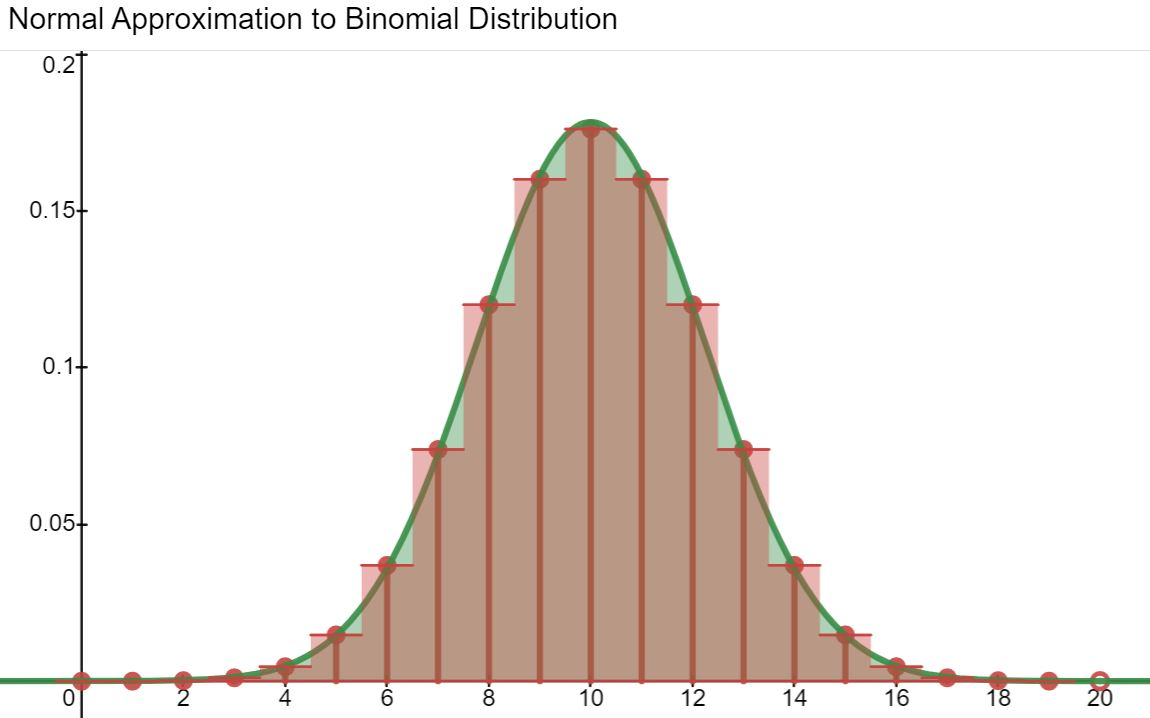
\includegraphics[width=0.75\linewidth]{./figures/normapprox} 

}

\caption{t distributions with 1, 5 and 20 degrees of freedom}\label{fig:napprox}
\end{figure}

\begin{example}
Approximate the probability of getting between \(8\) and \(12\) heads when tossing \(20\) fair coins.

\emph{solution}
\[Y \sim \text{Bin}(20,0.5) \approx X\sim \text{N}(10,0.5)\]

The exact probability is \(\text{P}(Y\leq 12) - \text{P}(Y\leq 7) = 0.7368\)

With a continuity correction:

\[\text{P}(8\leq X\leq12) = \text{P}\left(\frac{8-0.5-10}{\sqrt{5}} \leq Z \leq \frac{12+0.5-10}{\sqrt{5}} \right) \]
\[=\text{P}(-1.118\leq Z \leq 1.118)\]
\[=0.7364\]
\end{example}

\begin{example}
A galton board has small ball bearings that are released from an internal cavity to roll down a board. The board has small pins and when the ball bearing hits a pin, it will move to the left or the right of that pin. The distribution of the pins at the base of the instrument can be seen to follow a bell-curve empirically.
\end{example}

\hypertarget{proportions}{%
\subsection{Proportions}\label{proportions}}

Rather than using the normal approximation for \(X\) directly, we often want to estimate a proportion. This is the number out of the total number \(\frac{X}{n}\).

If \(X\sim \text{Bin}(n,\pi)\) is approximated by \(\text{N}(n\pi,n\pi(1-\pi))\), then what happens to the mean and variance if we want an approximation for \(X/n\)?

\[\text{E}\left(\frac{X}{n}\right) = \frac{1}{n}\text{E}(X)=\frac{1}{n}\times n\pi = \pi\]

\[\text{Var}\left(\frac{X}{n}\right) = \frac{1}{n^2}\text{Var}(X)\]

\[= \frac{1}{n^2}\times n\pi(1-\pi) = \frac{\pi(1-\pi)}{n}\]
So to approximate a proportion we use \(\text{N}(\pi,\frac{\pi(1-\pi)}{n})\)

\begin{definition}
A confidence interval for the population proportion \(\pi\) is given by the following expression

\[\left(p - z_{\alpha/2}\sqrt{\frac{p(1-p)}{n}}, p + z_{\alpha/2}\sqrt{\frac{p(1-p)}{n}}\right)\]
Where \(p\) is the observed proportion.
\end{definition}

This can be seen as

\begin{example}
An importer has ordered a large consignment of tomatoes. When it arrives he examines a randomly chosen sample of \(50\) boxes and finds that \(12\) contain at least one bad tomato. Assuming that these boxes may be regarded as being a random sample from the boxes in the consignment, obtain an approximate \(99\%\) confidence interval for the proportion of boxes containing at least one bad tomato, giving your confidence limits to three decimal places.
\end{example}

\emph{solution}

We have \(p=0.24\) and \(1-p = 0.76\). The relevant quantile is \(2.576\), so the confidence interval is

\[0.24 \pm 2.576\sqrt{\frac{0.24\times 0.76}{50}} = (0.084,0.396) \]

So approximately \(8\%\) to \(40\%\).

\hypertarget{summary}{%
\section{Summary}\label{summary}}

A confidence interval can be constructed from a sample or summary statistics. There are four types of confidence interval we have considered this week:

\begin{enumerate}
\def\labelenumi{\arabic{enumi})}
\item
  confidence interval for the mean with variance known.
  \[\left( \bar{x}-z_{\frac{\alpha}{2}}\frac{\sigma}{\sqrt{n}},\bar{x}+z_{\frac{\alpha}{2}}\frac{\sigma}{\sqrt{n}} \right) \]
\item
  confidence interval for the mean with variance \emph{unknown}.
  \[\left( \bar{x} - t_{n-1,\alpha /2} \frac{s}{\sqrt{n}}, \bar{x} + t_{n-1,\alpha /2} \frac{s}{\sqrt{n}}\right)  \]
\item
  confidence interval for an unknown variance.
  \[\left( \frac{(n-1)s^2}{\chi^2_{n-1,\alpha / 2}} \ , \ \frac{(n-1)s^2}{\chi^2_{n-1,1-\alpha / 2}}\right) \]
\end{enumerate}

You can take the square root endpoints for standard deviation.

\begin{enumerate}
\def\labelenumi{\arabic{enumi})}
\setcounter{enumi}{3}
\tightlist
\item
  confidence interval for a population proportion.
\end{enumerate}

\[\left(p - z_{\alpha/2}\sqrt{\frac{p(1-p)}{n}}, p + z_{\alpha/2}\sqrt{\frac{p(1-p)}{n}}\right)\]

We used \emph{unbiased estimates} for the mean and variance

\begin{enumerate}
\def\labelenumi{\arabic{enumi}.}
\item
  \[\bar{x} = \frac{1}{n}\sum_{i=1}^n x_i\]
\item
  \[s^2 = \frac{1}{n-1}\sum_{i=1}^n (x_i - \bar{x})^2 \]
\end{enumerate}

\[=\frac{1}{n-1}\left\{\sum_{i=1}^nx_i^2 - \frac{\left(\sum_{i=1}^n x_i\right)^2}{n} \right\} \]
- A binomial distribution \(\text{Bin}(n,p) \approx \text{N}(np, np(1-p))\).

\hypertarget{exercises-week-7}{%
\section{Exercises week 7}\label{exercises-week-7}}

\begin{exercise}

A random sample of size \(25\) is taken from a normal distribution with standard deviation \(4\). The sample mean is \(85\).

\begin{enumerate}
\def\labelenumi{\alph{enumi}.}
\item
  Find a 90\% confidence interval for the mean of the distribution.
\item
  Find a 95\% confidence interval for the mean of the distribution.
\item
  Find a 99\% confidence interval for the mean of the distribution.
\item
  Compare the intervals you calculated in a-c.
\end{enumerate}

\end{exercise}

\begin{exercise}

A random sample of \(20\) lobster traps gave the following results:

\begin{longtable}[]{@{}c@{}}
\toprule
Weights (lb)\tabularnewline
\midrule
\endhead
\(17.4, \ \ \ \  18.9, \ \ \ \ 39.6, \ \ \ \ 34.4, \ \ \ \  19.6\)\tabularnewline
\(33.7 , \ \ \ \  37.2, \ \ \ \  43.4, \ \ \ \  41.7, \ \ \ \  27.5\)\tabularnewline
\(24.1, \ \ \ \  39.6, \ \ \ \  12.2, \ \ \ \  25.5, \ \ \ \  22.1\)\tabularnewline
\(29.3, \ \ \ \  21.1, \ \ \ \  23.8, \ \ \ \  43.2, \ \ \ \  24.4\)\tabularnewline
\bottomrule
\end{longtable}

\begin{enumerate}
\def\labelenumi{\alph{enumi})}
\item
  Construct a \(95\%\) confidence interval for the mean weight of a catch.
\item
  What assumptions are necessary for the interval to be valid, one distributional and one otherwise.
\item
  Give an example of how these assumptions may not be valid in context.
\item
  The government have made some policies to reduce over-fishing. Historical records have that the mean catch is \(30.31\)lb. Is there evidence that the government policy has been effective?
\end{enumerate}

\end{exercise}

\begin{exercise}
Human body temperature can be modelled by a normal distibution with mean \(\mu\) and variance \(\sigma^2\). Emily, a medical student measured the body temperature of a random sample of \(20\) patients in a hospital.

She calculated a \(90\%\) confidence interval to be \((35.2,41.8)\).

Using Emily's sample and interval, calculate a \(99\%\) confidence interval.
\end{exercise}

\begin{exercise}

A random sample of size \(25\) is taken from a normal population with standard deviation \(2.5\).
The mean of the sample is \(17.8\).

\begin{enumerate}
\def\labelenumi{\alph{enumi}.}
\item
  Find a \(99\%\) C.I. for the population mean \(\mu\).
\item
  What size sample is required to obtain a \(99\%\) C.I. of width of at most \(1.5\)?
\item
  What confidence level would be associated with the interval based on the above sample of \(25\) but of width \(1.5\), i.e.~\((17.05, 18.55)\)?
\end{enumerate}

\end{exercise}

\begin{exercise}

The masses (in grams) of \(10\) nails selected at random from a bin of \(90\) mm long nails were:
\[9.7, \ \ 10.2, \ \  11.2, \ \  9.4, \ \  11.0, \ \  11.2, \ \  9.8, \ \  9.8, \ \  10.0, \ \  11.3\]
a. Calculate a 98\% confidence interval for the mean mass of the nails in the bin.

\begin{enumerate}
\def\labelenumi{\alph{enumi}.}
\setcounter{enumi}{1}
\tightlist
\item
  State one assumption you have made in your calculation.
\end{enumerate}

\end{exercise}

\begin{exercise}
A random sample of the feet of \(8\) adult males gave the following summary
statistics of length \(x\) (in cm):

\[\sum x = 224.1 , \ \ \ \ \ \ \sum x^2 = 6337.39 \]
Assuming that the length of men's feet is normally distributed, calculate a \(99\%\)
confidence interval for the mean length of men's feet based upon these results.
\end{exercise}

\begin{exercise}

A random sample of \(50\) one pound coins were weighed at the Royal Mint. It was found that the weights in grams were summarised by:

\[\sum x = 474.51 , \ \ \ \ \ \ \sum x^2 = 4503.8276 \]
a) Calculate unbiased estimates for the mean and variance.

\begin{enumerate}
\def\labelenumi{\alph{enumi})}
\setcounter{enumi}{1}
\item
  Find a \(t\)-distribution value and a \(z\)-value. Compare these.
\item
  Calculate a \(90\%\) confidence interval for the mean weight of a pound coin.
\item
  Estimate the size of a random sample required to give an interval of half the width of that calculated in the previous question.
\item
  It was later found that the scales were consistently underweighing by \(0.05\) grams. Which of the results of a), b) and d) will need amending, and which will be the same? Calculate the amended values.
\end{enumerate}

\end{exercise}

\begin{exercise}
A new variety of small daffodil is grown in the trial ground of a nursery. During the flowering period, a random sample of \(10\) flowers was taken and the lengths, in millimetres, of their stalks were measured. The results were as follows:
\[266, \ \ 254, \ \  215, \ \  220, \ \  253, \ \  230, \ \  216, \ \  248,  \ \ 234, \ \  244\]
Assuming that the lengths are normally distributed, calculate a \(95\%\) confidence interval for the variance of the lengths.
\end{exercise}

\begin{exercise}
A random sample of \(1000\) voters are interviewed, of whom \(349\) state they support the Conservative party. Determine an approximate \(98\%\) confidence interval for the proportion of Conservative supporters in the population.
\end{exercise}

\begin{exercise}

A market researcher performs a survey in order to determine the popularity of the washing powder brand ``SUDZ''. He visits every house on a large housing estate in the Manchester area and asks the question ``Do you use SUDZ washing powder?''. Of \(235\) people questioned, \(75\) responded in the positive.

\begin{enumerate}
\def\labelenumi{\alph{enumi})}
\item
  Calculate a \(95\%\) confidence interval for the proportion of households in the Manchester area that use SUDZ.
\item
  Comment on the sampling methodology, and how this may impact the validity of the interval.
\item
  Comment on whether the interview question is effective.
\end{enumerate}

\end{exercise}

\begin{exercise}

When a biased cubical die is rolled the probability that a six will be obtained is an unknown constant \(p\). The die is rolled \(40\) times and the number \(X\) of sixes obtained is recorded. The number \(Y\) of sixes obtained when the die is rolled a further \(60\) times is also recorded.

\begin{enumerate}
\def\labelenumi{\alph{enumi})}
\tightlist
\item
  Show that
\end{enumerate}

\[T_1 = \frac{3X+2Y}{240} \ \ \ \text{    and  } \ \ \ \ T_2 = \frac{X+Y}{100} \]
are both unbiased estimators for \(p\).
(Hint: find \(\text{E}(T_1)\) and \(\text{E}(T_2)\))

\begin{enumerate}
\def\labelenumi{\alph{enumi})}
\setcounter{enumi}{1}
\item
  Find in terms of \(p\) the standard errors of \(T_1\) and \(T_2\)
\item
  Reflecting on your previous answer, which of these estimators do you consider better?
\end{enumerate}

\end{exercise}

\hypertarget{hypothesis-testing}{%
\chapter{Hypothesis testing}\label{hypothesis-testing}}

This week we will introduce the main method of statistical inference - the hypothesis test. We will formulate hypothesis tests, interpret and report the results of hypothesis tests for a mean and variance.

We will also understand how to test comparisons between population parameters.

\hypertarget{one-sample-tests}{%
\section{One sample tests}\label{one-sample-tests}}

The operation of a hypothesis tests can be summarised in the following steps:

\begin{enumerate}
\def\labelenumi{\arabic{enumi})}
\item
  Summarise competing ideas about population parameters in terms of two hypotheses, called \textbf{\emph{null}} and \textbf{\emph{alternative}} hypotheses. The null hypothesis represents your default position, and the alternative is what you wish to test.
\item
  Choose a suitable test statistic, which assuming the null hypothesis should have a known distribution. Calculate the value of this test statistic, comparing it to a critical value of the known distribution. Or calculate the probability of the test statistic at least as extreme as that observed in the sample (p-value).
\item
  On the basis of this probability, decide whether there is evidence to reject the null hypothesis.
\end{enumerate}

Because of step (2) the conclusion of a hypothesis test is never \(100\%\) true. Statistical inference does not involve black and white absolute truths, but is rather more subtle.

\hypertarget{test-for-mean-known-variance}{%
\subsection{test for mean (known variance)}\label{test-for-mean-known-variance}}

In this section we will test hypotheses about the population mean \(\mu\) of a normal distribution.

How we implement the test depends on the hypotheses that we are testing.

\begin{example}
Each year trainees throughout the country sit a test. Over a period of time it has been established that the number of marks can be modelled by a normal distribution with mean \(70\) and standard deviation \(6\) marks.

This year it was thought that trainees from Greater Manchester performed better than expected.

A random sample of \(25\) trainees from Manchester had an average mark of \(\bar{x}=73.2\).

Does this provide evidence, at the \(5\%\) significance level, that the trainees from Greater Manchester did better than the national average?
\end{example}

\emph{solution}

\begin{enumerate}
\def\labelenumi{\arabic{enumi}.}
\tightlist
\item
  \emph{State your hypotheses}
\end{enumerate}

\[\text{H}_0: \ \mu = 70 \\  \text{H}_A: \ \mu > 70\]

\begin{enumerate}
\def\labelenumi{\arabic{enumi}.}
\setcounter{enumi}{1}
\tightlist
\item
  \emph{Choose test statistic}
\end{enumerate}

Here the statistic is \(\bar{X}\) and recall \(\bar{X}\sim\text{N}(\mu,6^2/25)\). Assuming \(\text{H}_{0}\), then \(\mu=70\). So we have the distribution: \[\bar{X}\sim\text{N}(70,1.44)\]

We calculate the standardised value of the observed sample mean

\[\frac{\bar{x} - 70}{\sigma /\sqrt{ n}}=\frac{73.2 - 70}{1.2} = 2.67\]
And compare this to the \(z\)-value with \(5\%\) in the upper tail, which you can find in the inverse normal tables. (Why the upper tail? Because \(H_{A}\) has a \(>\) in). See picture below.

\begin{figure}

{\centering 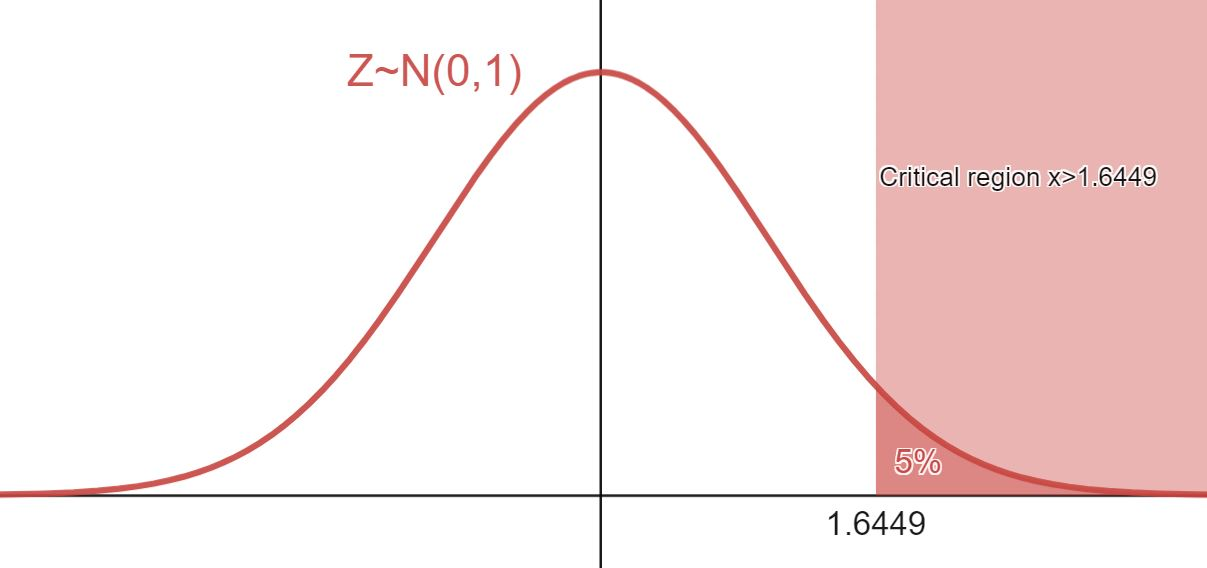
\includegraphics[width=0.75\linewidth]{./figures/criticalregion} 

}

\caption{critical region}\label{fig:crit1}
\end{figure}

\begin{enumerate}
\def\labelenumi{\arabic{enumi}.}
\setcounter{enumi}{2}
\tightlist
\item
  \emph{Decision}
  Now \(2.6667 > 1.6449\), this value of the sample mean is in the critical region. The interpretation is that a value as extreme as this or worse is sufficiently unlikely (\(<5\%\)), so we are able to reject \(\text{H}_{0}\).
\end{enumerate}

It is important that the sample is random, as otherwise this invalidates the conclusion. For example if these \(25\) were particularly high attainers, then it would not be representative of the distribution, and \(\bar{x}\) may have been smaller in a representative sample.

In the example above we compare positive values, and the critical region is in the left tail of the distribution.

\begin{definition}
We say a hypothesis test is \textbf{\emph{right-tailed}} if it is of the form:
\[\text{H}_A: \ \mu > \mu_0\]
A hypothesis is \textbf{\emph{left-tailed}} if it is of the form:

\[\text{H}_A: \ \mu < \mu_0\]

And \textbf{\emph{two-tailed}} if it is of the form:
\[\text{H}_A: \ \mu \neq \mu_0\]
\end{definition}

This is a table for the decision process

\begin{longtable}[]{@{}cc@{}}
\toprule
\(\text{H}_{A}\) & Reject \(H_{0}\) if\tabularnewline
\midrule
\endhead
\(H_{A}: \mu > \mu_0\) & \(Z>z_{\alpha}\)\tabularnewline
\(H_{A}: \mu < \mu_0\) & \(Z<-z_{\alpha}\)\tabularnewline
\(H_{A}: \mu \neq \mu_0\) & \(|Z|>z_{\frac{1}{2}\alpha}\)\tabularnewline
\bottomrule
\end{longtable}

\begin{example}
In the testing example suppose the sample mean had been \(\bar{x}=69.5\), and we wished to test at the \(5\%\) level if the mean is different from \(70\). That is:

\[\text{H}_0: \ \mu = 70 \\  \text{H}_A: \ \mu \neq 70\]
\emph{solution}

We calculate the test statistic as before:

\[\frac{\bar{x}-\mu_0}{\sigma / \sqrt{n}} =\frac{69.5-70}{1.2}=-0.4167  \]
The alternative hypothesis \(\neq\) includes left \(>\) and right \(<\) tails. Now \(5\%\) is in both tails, so \(5\% / 2 =2.5\%\) in either tail.

Using tables we find that \(z_{2.5\%} = 1.960\). We would reject if the test statistic were greater than \(1.96\) or if the test statistic were smaller than \(-1.96\). Equivalently we would reject \(\text{H}_0\) if the modulus exceeds 1.96, that is \[|\text{ test statistic}|>1.96.\]

Here
\[|-0.4167| = 0.4167 \ngtr 1.96,\]
so there is insufficient evidence to reject \(\text{H}_0\).
\end{example}

Recall the interpretation of this conclusion is never definitive. We never accept the null hypothesis, but rather fail to reject it. It may be that with further data we pass the threshold of the critical value and are able to reject the null hypothesis.

A two-sided alternative hypothesis is similar to a confidence interval.

If a confidence interval with confidence level \(c\%\) excludes the population value of interest, then the null hypothesis that teh population parameter takes this value will be rejected at the \(100(1-c)\%\) level.

\begin{example}
Suppose a \(95\%\) confidence interval for the mean \(\mu\) is \((83.0,85.1)\), then the null hypothesis that \(\mu=85.2\) will be rejected at the \(5\%\) level since the interval excludes \(85.2\). Indeed any hypothesised value outside the interval will be rejected at the \(5\%\) level.
\end{example}

\hypertarget{test-for-mean-unknown-variance}{%
\subsection{test for mean (unknown variance)}\label{test-for-mean-unknown-variance}}

When the population variance (\(\sigma^2\)), or equivalently the population standard deviation \(\sigma\), is \emph{unknown} we must estimate it from the sample.

For small samples the distribution of the test statistic follows a \(t\)-distribution.

If the null hypothesis is given by \(\text{H}_0: \mu = \mu_0\), the test statistic is given by

\[T = \frac{\bar{x}-\mu_0}{s/\sqrt{n}}\sim t_{n-1}\]
The decision rules are essentially the same but with \(z_\alpha\) and \(z_{\alpha/2}\) replaced by the same quantiles of the t-distribution \(t_{n-1,\alpha}\) and \(t_{n-1,\alpha}\), respectively. Further \(\sigma\) is estimated by \(s\).

\begin{longtable}[]{@{}cc@{}}
\toprule
\(\text{H}_{A}\) & Reject \(H_{0}\) if\tabularnewline
\midrule
\endhead
\(H_{A}: \mu > \mu_0\) & \(T>t_{\alpha}\)\tabularnewline
\(H_{A}: \mu < \mu_0\) & \(T<-t_{\alpha}\)\tabularnewline
\(H_{A}: \mu \neq \mu_0\) & \(|T|>t_{\frac{1}{2}\alpha}\)\tabularnewline
\bottomrule
\end{longtable}

Where \(t_{\alpha}\) and \(t_{\alpha/2}\) are obtained from \(t\)-tables with degrees of freedom \(\nu = n-1\), and the sample variance is given by, for example,

\[s^2 =\frac{1}{n-1}\sum_{i=1}^{n}(x_i-\bar{x})^2.\]

\begin{example}

A shopkeeper sells jars of jam. The weights of the jars of jam are normally distributed with a mean of \(150\)g. A customer complains that the mean weight of a pack of\(8\) jars she had bought was only \(147\)g. An estimate for the standard deviation of the weights of the \(8\) jars of jam calculated from the \(8\) observations was \(2\)g.

\begin{enumerate}
\def\labelenumi{\alph{enumi})}
\item
  Test at the \(5\%\) significance level whether \(147\)g is significantly less than the quoted mean.
\item
  Discuss whether the customer has cause for complaint.
\end{enumerate}

\emph{solution}

\begin{enumerate}
\def\labelenumi{\alph{enumi})}
\item
\end{enumerate}

\[H_{0}: \mu = 150 \\ \text{H}_A: \mu<150\]

Significance level \(=0.05\), left-tailed test.

Degrees of freedom \(\nu = 8-1 = 7\).

From tables \(t_{7, \ 5\%} = -1.895\)

We reject \(H_0\) if the statistic is less than \(-1.895\)

\[T =\frac{\bar{x}-\mu}{s/\sqrt{n}}=\frac{147-150}{2/\sqrt{8}}=-4.2426 \]
Now \(-4.2426 < -1.895\), the result is significant and \(H_0\) is rejected.

\begin{enumerate}
\def\labelenumi{\alph{enumi})}
\setcounter{enumi}{1}
\tightlist
\item
  There is evidence to suggest that the mean weight is less than \(150\)g, supporting the customer complaint. However one pack is not a random sample, so it could be a bad batch not that all the jars are being under-filled.
\end{enumerate}

\end{example}

The distribution of \(T\) is only a \(t\)-distribution when we assume a normally distributed population.

If the sample is large and so the degrees of freedom are increased, we still need to estimate and calculate \(s\), but often a \(z\)-value can be used in practice. Strictly speaking a \(t\)-value should be used in place of a \(z\)-value whenever \(s\) is used in place of \(\sigma\) and not just because \(n\) is small.

\hypertarget{test-for-variance}{%
\subsection{test for variance}\label{test-for-variance}}

If you have a random sample of observations from a normal distribution with mean \(\mu\) and standard deviation \(\sigma\) where both are unknown, the sample variance is given by (for example) the formula

\[S^2 = \frac{1}{n-1}\sum_{i=1}^{n}(x_i-\bar{x})^2\]

Recall it can be shown that

\[\frac{(n-1)S^2}{\sigma^2}\sim\chi^2_{n-1}\]

To test against the null hypothesis that the variance is some particular value, that is
\[\text{H}_0: \sigma^2 = \sigma_0^2\]
We can just compare the expression \(\frac{(n-1)S^2}{\sigma^2}\), with the hypothesised population variance, to the relevant quantile of some chi-squared distribution. This gives the following decision rules:

\begin{longtable}[]{@{}cc@{}}
\toprule
\begin{minipage}[b]{0.43\columnwidth}\centering
\(\text{H}_{A}\)\strut
\end{minipage} & \begin{minipage}[b]{0.51\columnwidth}\centering
Reject \(H_{0}\) if\strut
\end{minipage}\tabularnewline
\midrule
\endhead
\begin{minipage}[t]{0.43\columnwidth}\centering
\(H_{A}: \sigma^2 > \sigma^2_0\)\strut
\end{minipage} & \begin{minipage}[t]{0.51\columnwidth}\centering
\(\frac{(n-1)S^2}{\sigma^2}>\chi^2_{\alpha, \ n-1}\)\strut
\end{minipage}\tabularnewline
\begin{minipage}[t]{0.43\columnwidth}\centering
\(H_{A}: \sigma^2 \neq \sigma^2_0\)\strut
\end{minipage} & \begin{minipage}[t]{0.51\columnwidth}\centering
\(\frac{(n-1)S^2}{\sigma^2}<\chi^2_{1-\frac{1}{2}\alpha, \ n-1}\) or \(\frac{(n-1)S^2}{\sigma^2}>\chi^2_{\frac{1}{2}\alpha, \ n-1}\)\strut
\end{minipage}\tabularnewline
\bottomrule
\end{longtable}

\begin{example}
A bus company is trying to improve their reliability, and so the consistency with respect to the schedule is monitored. The company wants the arrival time to have standard deviation \(2\) minutes or less. A sample of \(10\) arrival times shows a sample variance of \(5\). Using a \(5\%\) signifiance level, does the data suggest that the variance in arrival times is meeting the company standard?

\emph{solution}
Our hypotheses are:
\[\text{H}_0: \sigma^2=4 \ \ \ , \ \ \ \text{H}_A: \sigma^2 >4\]
The test statistic is:
\[\frac{(n-1)S^2}{\sigma^2}=\frac{9\times5}{4} = 11.25\]
Our critical value is
\[\chi^2_{\alpha,n-1}=\chi^2_{0.05,9}=16.92\]
Since \(11.25\ngtr16.92\) we have insufficient evidence to reject \(\text{H}_0\). Therefore we are unable to conclude that the variance in bus arrival times is not meeting the company standard.
\end{example}

\hypertarget{p-value-approach}{%
\subsection{p-value approach}\label{p-value-approach}}

There are two ways of looking at the comparison involved to reject a null hypothesis, via the critical region or via p-values. The critical region is rather blunt and uninformative - we either reject or do not reject the null. However, the p-value allows us to quantify the weight of evidence against the null hypothesis given by the sample data. For many tests exact p-values can be calculated in R.

\begin{definition}
A \textbf{\emph{p-value}} is the probability of a observing the value of a statistic at least as extreme as that of the particular value of that statistic in the observed sample.

For example if a sample gives sample mean \(\bar{x}=101.3\) then the p-value would be \[p  =\text{P}(\bar{X}\geq101.3).\]
\end{definition}

We will illustrate an example with a right tailed test.

\begin{example}
Suppose we want to test the following:
\[\text{H}_0:\mu = 26.3 \ \ \ , \ \ \ \text{H}_A: \mu >26.3\]

Where:

\begin{longtable}[]{@{}cccc@{}}
\toprule
\(n\) & \(\bar{x}\) & \(\sigma\) & \(\alpha\)\tabularnewline
\midrule
\endhead
10 & 27 & 1.2 & \(5\%\)\tabularnewline
\bottomrule
\end{longtable}

\begin{enumerate}
\def\labelenumi{\alph{enumi})}
\item
  Perform the test
\item
  Calculate the p-value
\end{enumerate}

Here we can work out the \(z\)-value tobe \(1.6449\). The statistic is

\[\frac{27 - 26.3}{1.2/\sqrt{10}} = 1.845\]
And we would reject \(\text{H}_0\) as \(1.845 > 1.6449\).

\begin{enumerate}
\def\labelenumi{\alph{enumi})}
\setcounter{enumi}{1}
\item
\end{enumerate}

We know under the null hypothesis that \(\bar{X} \sim \text{N}(26.3, 1.2^2/10)\).

The p-value is the probability of observing a particular value at least as extreme as \(\bar{x}=27\).

You could use the distribution of \(\bar{X}\) directly or the already standardised value above and find \[p = \text{P}(\bar{X} >27) = \text{P}(Z>1.845) = 0.0325 \]
\end{example}

In the example above the p-value is \(0.0325\) and the significance level was \(5\%\). The p-value can be compared to the significance level directly to conclude a hypothesis test. If the p-value is lower than the significance level, then we can reject the null hypothesis.

The statistic is \emph{greater} than the critical value only when the p-value (tail probability) is \emph{less} than the significance level. See the following picture:

\begin{figure}

{\centering 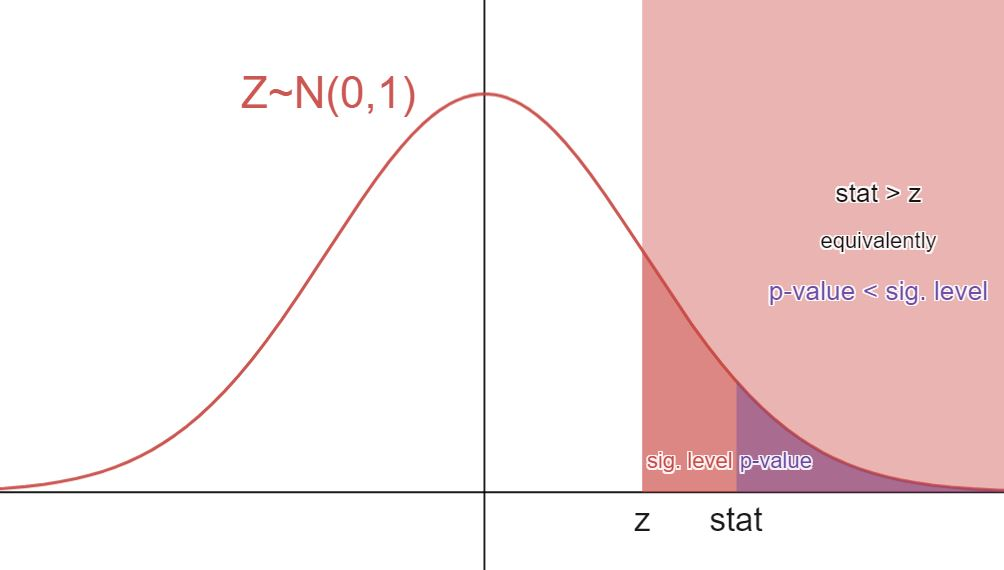
\includegraphics[width=0.75\linewidth]{./figures/p-value} 

}

\caption{critical region}\label{fig:pval}
\end{figure}

For tests involving the t-distribution or the chi-squared distribution, the p-value is in practice obtained via software such as R, and we will see this in labs this week.

Usually the p-value is compared to \(5\%\) however, there are standard interpretations of p-values which quantify the evidence against \(\text{H}_0\).

\begin{longtable}[]{@{}cc@{}}
\toprule
p-value range & interpretation\tabularnewline
\midrule
\endhead
\(p>0.1\) & No evidence against H\(_0\), or data consistent with H\(_0\)\tabularnewline
\(0.05 < p < 0.1\) & Weak evidence against H\(_0\)\tabularnewline
\(0.01 < p < 0.05\) & Some evidence against H\(_0\)\tabularnewline
\(0.001 < p < 0.01\) & Strong evidence against H\(_0\)\tabularnewline
\(0.001 < p < 0.01\) & very strong evidence against H\(_0\)\tabularnewline
\bottomrule
\end{longtable}

In formal reports if a significant effect is found, quantify the effect with a confidence interval. Phrasing of conclusions is important, always set in context (without jargon e.g.~H\(_0\)).

\hypertarget{types-of-error}{%
\subsection{types of error}\label{types-of-error}}

Any decision relying on imperfect information has to allow for the fact that there is uncertainty so the decision cannot be certain. There are two types of systematic uncertainty that arise from hypothesis testing, or types of error.

\begin{example}
Suppose a man is in court accused of murder. The decision that the judge or jury come to is separate from the truth of the guilt or innocence of the man.

\[\ \ \ \ \text{H}_0: \text{the man is innocent} \\ \text{H}_1: \text{the man is guilty}\]
The trial process is like an hypothesis test in which the evidence presented is equivalent to the data. The possible decisions are summarised in the table below:

\begin{longtable}[]{@{}ccc@{}}
\toprule
& Innocent & Not innocent\tabularnewline
\midrule
\endhead
Accept innocence & & x\tabularnewline
Reject innocence & x &\tabularnewline
\bottomrule
\end{longtable}

It would be undesirable to sentence an innocent man, or to find set a guilty man loose.
\end{example}

\begin{definition}

There are two types of error which are systematic to hypotheis testing.

A \textbf{\emph{type I error}} is to reject the null hypothesis when it is, in fact true.

A \textbf{\emph{type II error}} is to accept the null hypothesis when it is in fact false.

\begin{longtable}[]{@{}ccc@{}}
\toprule
& H\(_0\) true & H\(_0\) false\tabularnewline
\midrule
\endhead
Accept \(H_0\) & & II\tabularnewline
Reject \(H_0\) & I &\tabularnewline
\bottomrule
\end{longtable}

\end{definition}

The probabilities of each type of error are important, we would seek to minimise both if possible.

\begin{definition}
The \textbf{\emph{significance level}} of the test is the probability of type I error.
\[\text{P}(\text{Type I error}) = \text{P}(\text{H}_0 \text{ rejected} | \text{H}_0 \text{ is true})\]
If you are given the significance level for example \(5\%\), then this is the probability of type I error. However this may not always be stated in a question and you may have to work it out.
\end{definition}

\begin{example}
A random variable has a normal distribution with mean µ and standard deviation \(3\).
The null hypothesis \(\mu=20\) is to be tested against the alternative hypothesis \(\mu>20\) using a random sample of \(25\).
It is decided that the null hypothesis will be rejected if the sample mean is greater than \(21.4\).
Calculate the probability of making a type I error.

\emph{solution}

\[\text{P}(\text{Type I error}) = \text{P}(\text{H}_0 \text{ rejected} | \text{H}_0 \text{ is true})\]
\[=\text{P}(\bar{X} > 21.4 \ | \ \mu = 20)\]
This can be obtained, for example by standardising from tables,
\[=\text{P}\left(\frac{\bar{X}-20}{3/\sqrt{25}}>\frac{21.4-20}{3/\sqrt{25}} \right)\]
\[=\text{P}(Z>2.33) = 9.9\times 10^{-3} \approx 1\%\]
\end{example}

\begin{example}
The weight of jam in a jar, measured in grams, is distributed normally with a mean of \(150\)g and a standard deviation of \(6\)g. The production process occasionally leads to a change in the mean weight of jam per jar but the standard deviation remains unaltered. The manager monitors the production process and for every new batch takes a random sample of \(25\) jars and weighs their contents to see if there has been any \emph{reduction} in the mean weight of jam per jar.
Find the critical values for the test statistic \(\bar{X}\), the mean weight of jam in a sample of \(25\) jars, using

\begin{enumerate}
\def\labelenumi{\alph{enumi})}
\item
  5\% level of significance
\item
  1\% level of significance
\item
  Given that the true value of µ for the new batch is in fact 147g. Find the probability of a type II error for each of the above critical regions
\end{enumerate}

\emph{solution}
a) \(z_{5\%} = -1.6449\), so we would reject \(H_0\) if

\[\frac{\bar{x}-150}{6/\sqrt{25}}<-1.6449 \]
Rearranging this inequality gives \(\bar{x} < 148.03\)

\begin{enumerate}
\def\labelenumi{\alph{enumi})}
\setcounter{enumi}{1}
\item
  \(z_{1\%} = -2.326\) , rearranging a similar inequality gives \(\bar{x} < 147.208\ldots\)
\item
  Here you use the distribution \(\bar{X}\sim\text{N}(147, 6^2/\sqrt{25})\). Type II error is where we do not reject \(H_0\) so we reverse the inequalities from the regions above and evaluate the probabilities:
\end{enumerate}

\[\text{P}(\bar{x} \geq 148.03 | \ \mu = 147) = 0.195 \approx 20\%\]

\[\text{P}(\bar{x} \geq 147.2 | \ \mu = 147) = 0.4309\ldots \approx 43\%\]
\end{example}

When we reduce the P(Type I error) from 5\% to 1\%, P(Type II error) increased from \(\approx 20\%\) to \(43\%\). So just reducing the probability of one type of error is not a cure-all.

\hypertarget{two-sample-tests}{%
\section{Two sample tests}\label{two-sample-tests}}

We may wish to use hypothesis testing to compare two populations. The two populations may be the distributions of heights of males and females separately. Or we may wish to compare average the weights of babies born in one region to another.

Supposing we have two distributions \(X\) and \(Y\), we write the population parameters with a subscript to indicate to which distribution they correspond. The basic setup is as follows

\begin{longtable}[]{@{}ccc@{}}
\toprule
Parameter & Population 1 & Population 2\tabularnewline
\midrule
\endhead
Mean & \(\mu_X\) & \(\mu_Y\)\tabularnewline
Variance & \(\sigma^2_X\) & \(\sigma^2_Y\)\tabularnewline
\bottomrule
\end{longtable}

The main hypotheses of interest are whether or not the means are different. That is:

\[\text{H}_0: \mu_X = \mu_Y \ \ \ \ \ \ , \ \ \ \ \ \text{H}_A:\mu_X \neq \mu_Y\]

Though one-sided alternatives, or specified differences can also be used.

We will assume both populations are normally distributed and consider three different situations:

\begin{enumerate}
\def\labelenumi{\alph{enumi})}
\item
  The population variances are known
\item
  The population variances are unknown, but known to be or are assumed to be equal.
\item
  The population variances are unknown and cannot be assumed to be equal.
\end{enumerate}

\hypertarget{known-variance}{%
\subsection{known variance}\label{known-variance}}

Assume we have a random sample \(x_1,x_2,\ldots,x_{n_1}\) of \(n_1\) observations from the first population, and another random sample \(y_1,y_2,\ldots, y_{n_2}\) of \(n_2\) observations from the second population.

The test statistic here is \(\bar{X}-\bar{Y}\).

Recall that the sampling distribution of the mean takes the form:
\[\bar{X} \sim \text{N}(\mu_X, \sigma^2_X / n_1) \ \ \ \ \ \ , \ \ \ \ \bar{Y} \sim \text{N}(\mu_Y, \sigma^2_Y / n_2)\]
Then, as the difference of normal distributions is again normal, with linearity of the expectation and variance the sum of the variances we have:

\[\bar{X}-\bar{Y} \sim \text{N}\left(\mu_X-\mu_Y , \frac{\sigma_X^2}{n_1} + \frac{\sigma_Y^2}{n_2}\right)\]
The test statistic is the standardised value of this statistic:

\[Z = \frac{\bar{X} - \bar{Y} - (\mu_X-\mu_Y)}{\sqrt{\frac{\sigma_X^2}{n_1} + \frac{\sigma_Y^2}{n_2}}}\]
\[\sim\text{N}(0,1).\]
Now under the null hypothesis \(\mu_X-\mu_Y = 0\), so this simplifies to:

\[\frac{\bar{X} - \bar{Y}}{\sqrt{\frac{\sigma_X^2}{n_1} + \frac{\sigma_Y^2}{n_2}}}\]
And we have the same decision rules as before.

\begin{example}
The weights of boys and girls of a particular age are known to be normally distributed with standard deviations \(5\)kg and \(8\)kg respectively. In a particular school, a random sample of \(25\) boys had mean weight \(48\)kg and a random sample of \(30\) girls had mean weight \(45\)kg.

Test, at the \(5\%\) significance level, whether there is evidence that the mean weight of the boys is greater than that of the girls.

\emph{solution}

\[\text{H}_0: \mu_B = \mu_G \ \ \ \ \ \ , \ \ \ \ \ \text{H}_A:\mu_B > \mu_G\]

We have
\[\frac{\bar{B}-\bar{G}}{\sqrt{\frac{\sigma_B^2}{n_1} + \frac{\sigma_G^2}{n_2}}}= \frac{48-45}{\sqrt{\frac{5^2}{25}+\frac{8^2}{30}}}= 1.69747\ldots \]
The critical value is \(1.6449\)
Hence here we reject the null hypothesis and conclude there is sufficient evidence to say that the boys weigh more than the girls on average.
\end{example}

\hypertarget{unknown-equal-variance}{%
\subsection{unknown equal variance}\label{unknown-equal-variance}}

In this section we know or can assume that the variances are equal. We may know outright that the variances are equal, even if they are unknown. For example, if I take a sample of men's heights from Manchester and compare to a sample of men's heights in London. It may be that there are average height differences, but as both are UK adult men they come from the same containing population, can be assumed to be just as variable as each other.

In this case we do not know \(\sigma_X^2\) or \(\sigma_Y^2\), so we will have to estimate each of these from actual data. We can estimate each by

\[s_x^2 = \frac{1}{n_1}\sum_{i=1}^n(x_i-\bar{x})^2 \ \ \ \ , \ \ \ \ s_y^2 = \frac{1}{n_2}\sum_{j=1}^n(y_j-\bar{y})^2 \]

But now we have two estimates for the unknown population variances \(\sigma_x^2, \ \sigma_y^2\). But we know, or can assume, these are equal to a common population variance \(\sigma_x^2=\sigma_y^2=\sigma^2\). The solution to this is to `pool' the variance using the formula:

\[s_p^2  = \frac{(n_1-1)s_x^2+(n_2-1)s_y^2}{n_1+n_2-2}\]
The test statistic is then calculated as,

\[T = \frac{\bar{X}-\bar{Y}}{s_p\sqrt{\frac{1}{n_1}+\frac{1}{n_2}}} \sim t_{n_1+n_2-2} \]
which follows a t distribution on \(n_1+n_2-2\) degrees of freedom.

\begin{example}

The heights (measured to the nearest centimetre) of a random sample of six policement from a certain force in Wales were found to be
\[176, \ 180, \ 179, \ 181, \ 183, \ 179.\]
The heights of a random sample of \(11\) policemen from Scotland gave the following data

\[\sum y =1991  \ \ \ \ , \ \ \ \sum(y-\bar{y})^2 = 54\]
a) Test at the \(5\%\) level the hypothesis that the Welsh policemen are shorter than the Scottish policemen.

\begin{enumerate}
\def\labelenumi{\alph{enumi})}
\setcounter{enumi}{1}
\tightlist
\item
  What assumptions are necessary for part (a)?
\end{enumerate}

\end{example}

\emph{solution}

The hypotheses are
\[\text{H}_0: \mu_{x} = \mu_{y} \ \ \ \ , \ \ \ \text{H}_A: \mu_{x}< \mu_{y}\]
From the question:

\[\bar{x}=179.66667, \ \ s^2_x =5.46667 \]

\[\bar{y}= 1991/11 = 181, \ \ \ s^2_y = 54/10 = 5.4 \]
We observe that 5.4 and 5.47 are approximately equal, so it is reasonable to pool these.

\[s^2_p = \frac{(6-1)\times5.46667 +(11-1)\times5.4 }{6+11-2} =5.422\ldots\]
Giving a pooled standard deviation of \(\sqrt{5.422} = 2.329\).
(you want to work a bit more accurately than the accuracy of the critical value you will be comparing to)

Now evaluating the test statistic:

\[\frac{179.66 - 181}{2.329\sqrt{\frac{1}{6}+\frac{1}{11}}} =  -1.128\]
We compare this to \(t_{15, 0.05} = 1.7531\)

Comparison: \(|-1.128|\ngtr 1.7531\)

There is insufficient evidence based on these samples to conclude that the population of Welsh officers are shorter than the population of Scottish officers.

\hypertarget{testing-for-equal-variance}{%
\subsection{testing for equal variance}\label{testing-for-equal-variance}}

In this situation we have two sample variances \(S^2_x\) and \(S^2_y\), and we want to determine by means of a hypothesis test if these are equal or not. Of course the conclusion is not definite, but in practice this informs whether we will pool the variances or not.

The null hypothesis is that the variances are equal, with the usual alternatives.

\[\text{H}_0: \sigma^2_x = \sigma^2_y\ \]

First a recap. We know that when scaled, sample variances follow a \(\chi^2\)-distribution. That is,

\[\frac{(n_1-1)S^2_x}{\sigma^2_x}\sim \chi^2_{n_1-1} \ \ \ , \ \ \  \frac{(n_2-1)S^2_y}{\sigma^2_y}\sim \chi^2_{n_2-1}\]

There is another distribution we must define, and this will be the last for the statistical tables.

\begin{definition}
Let \(X\sim \chi^2_n\) and \(Y\sim \chi^2_m\) then the following ratio defines an F-distribution with degrees of freedom \(n\) and \(m\). That is:

\[\frac{\left(\frac{X}{n}\right)}{\left(\frac{Y}{m}\right)}\sim \text{F}_{n,m}\]
\end{definition}

In our situation this tells us that under the null hypothesis we have

\[\frac{S^2_x}{S^2_y}\sim \text{F}_{n_1 - 1,n_2-1} \]
:::\{.example\}
A manufacturer of wooden furniture stores some of its wood outside and some inside a special
store. It is believed that the wood stored inside should have less variable hardness properties than that stored outside. Some \(25\) pieces of wood stored outside was taken and compared to \(21\) similar pieces taken from the inside store, with the following results:

\begin{longtable}[]{@{}ccc@{}}
\toprule
Value & Outside & Inside\tabularnewline
\midrule
\endhead
sample size & 25 & 21\tabularnewline
Mean hardness & 110 & 122\tabularnewline
\(\sum(x-\bar{x})^2\) & 5190 & 3972\tabularnewline
\bottomrule
\end{longtable}

\begin{enumerate}
\def\labelenumi{\alph{enumi})}
\item
  Test at the \(5\%\) significance level whether the manufacturer's belief is correct.
\item
  State two assumptions necessary to carry out this test.
\end{enumerate}

\emph{solution}

\begin{enumerate}
\def\labelenumi{\alph{enumi})}
\tightlist
\item
  We wish to test
\end{enumerate}

\[\text{H}_0: \sigma^2_x=\sigma^2_y \ \ \ , \ \ \ \text{H}_A: \sigma^2_x>\sigma^2_y\]
Working out the sample variances gives

\[s^2_x = \frac{5190}{25}=216.25, \ \ \ s^2_y = \frac{3972}{20} = 198.6\]
The test statistic is then

\[216.25/198.6 = 1.089,\]
which we compare to \(\text{F}_{24,20} = 2.08\).

Now, \(1.089 < 2.08\) so there is insufficient evidence to reject \(\text{H}_0\). So the wood from outside is just as variable as the wood inside.

\begin{enumerate}
\def\labelenumi{\alph{enumi})}
\setcounter{enumi}{1}
\tightlist
\item
  The assumption is that both populations are normal, and that the samples are independent and random.
  :::
\end{enumerate}

\hypertarget{unknown-unequal-variances-non-examinable}{%
\subsection{unknown unequal variances (non-examinable)}\label{unknown-unequal-variances-non-examinable}}

If we want to carry out a \(2\) sample \(t\)-test without assuming equal population variances we can use \[T = \frac{\bar{X} - \bar{Y}}{\sqrt{\frac{S_X^2}{n_1} + \frac{S_Y^2}{n_2}}}\]

However the distribution of this quantity is in general not of a convenient closed-form (analytic). As such it is actually a famous an unsolved problem generally, called the Behrens--Fisher problem. However it is approximately a \(t_\nu\)-distribution with degrees of freedom \(\nu\) given by the integer part of the following expression.

\[\frac{\left[\frac{S^2_x}{n_1}+\frac{S^2_y}{n_2} \right]^2}{\frac{1}{(n_1-1)}\left[\frac{S_x^2}{n_1}\right]^2+\frac{1}{(n_2-1)}\left[\frac{S_y^2}{n_2}\right]^2} \]

The above expression is known as the Welch approximation.

\begin{example}
A market inspector randomly samples the produce on two market stalls. A sample of \(80\) apples from Rufus Russett's stall had masses (in grams) having sample mean \(74.2\) and sample variance \(43.23\).
An independent random sample of \(100\) apples sold my Granny Smith had a sample mean of \(68.6\) and a sample variance of \(43.34\).

Test at the \(5\%\) significance level if there is evidence that the apples on Smith's stall have a lower average mass than Russett's stall.
\end{example}

\emph{solution}

We are testing
\[\text{H}_0: \mu_x = \mu_y \ \ \ , \ \ \text{H}_A:\mu_x>\mu_y\]
The test statistic is

\[ \frac{74.2 - 68.8}{\sqrt{\frac{24.21}{80}+\frac{43.23}{100}}} = 6.299\]
We want to compare this to \(t_\nu\). Let's evaluate the degrees of freedom here:

\[\frac{\left[\frac{24.21}{80}+\frac{43.23}{100} \right]^2}{\frac{1}{79}\left[\frac{24.21}{80}\right]^2+\frac{1}{99}\left[\frac{43.23}{100}\right]^2} = 177.26 \]
The integer value of this is \(177\), so we would check the critical value of a \(t_177\) distribution.

However \(177\) is a large number of degrees of freedom, so we use \(t_{\infty}=1.6448\) or \(z\)-value essentially, and the null is overwhelmingly rejected, as \(6.299 >1.6448\).

\hypertarget{summary-1}{%
\subsection{Summary}\label{summary-1}}

\begin{itemize}
\tightlist
\item
  A hypothesis test is a decision process about population parameters.
\end{itemize}

One sample tests we have learned about include:

\begin{itemize}
\item
  one sample \(z\)-test for the mean, known variance
  \[ \frac{\bar{x}-\mu_0}{\sigma/\sqrt{n}}\sim \text{N}(0,1) \]
\item
  one sample \(t\)-test, for the mean, unknown variance
  \[T = \frac{\bar{x}-\mu_0}{s/\sqrt{n}}\sim t_{n-1}\]
\item
  one sample test for variance
\end{itemize}

\[\frac{(n-1)S^2}{\sigma^2}\sim\chi^2_{n-1} \]

There are two types of systematic errors that occur when we test hypotheses, we typically limit the \emph{type I} error by setting the significance level.

We can compare two independent samples with:

\begin{itemize}
\tightlist
\item
  two sample \(z\)-test (known variances)
\end{itemize}

\[\frac{\bar{X} - \bar{Y}}{\sqrt{\frac{\sigma_X^2}{n_1} + \frac{\sigma_Y^2}{n_2}}}\sim \text{N}(0,1)\]

\begin{itemize}
\tightlist
\item
  two sample \(t\)-test (unknown equal variances) require pooled variance estimate:
\end{itemize}

\[T = \frac{\bar{X}-\bar{Y}}{s_p\sqrt{\frac{1}{n_1}+\frac{1}{n_2}}} \sim t_{n_1+n_2-2}\]
\[s_p = \frac{(n_1-1)s_x^2+(n_2-1)s_y^2}{n_1+n_2-2}\]

We can often assume the variances are equal. There is also a test for equality of variances.

\hypertarget{exercises-week-8}{%
\section{Exercises week 8}\label{exercises-week-8}}

\begin{exercise}

Jars of honey are filled by a machine. Over the lifetime of the machine, it has been found the quantity of honey has mean \(460.3\)g and standard deviation \(3.2\)g. It is believed that the machine has been altered so that the mean may have changed. \(60\) jars are taken and the mean quantity of honey per jar is found to be \(461.2\)g

\begin{enumerate}
\def\labelenumi{\alph{enumi})}
\item
  State suitable null and alternative hypotheses
\item
  Carry out a test using a \(5\%\) level of significance.
\item
  State two assumptions required for this test, and give an example of how each may not hold true.
\end{enumerate}

\end{exercise}

\begin{exercise}
The distance driven by a long distance lorry driver in a week is a normally distributed variable with mean \(1130\)km and standard deviation \(106\)km. New driving regulations are introduced and, in the first \(20\) weeks he drives a total of \(21900\)km. Assuming the standard deviation has not changed since the new regulations, test at the \(10\%\) level of significance whether the mean weekly distance has reduced. State clearly your null and alternative hypotheses.
\end{exercise}

\begin{exercise}
After a nuclear accident,government scientists measured radiation levels at \(20\) randomly chosen sites in a small area. The measuring instrument used is calibrated so as to measure the ratio of present radiation to the previous known average radiation in that area. The measurements are summarised by

\[\sum x = 22.8 \ \ , \ \ \sum x^2 = 27.55\]
Making suitable assumptions test, at the \(5\%\) level, the hypothesis that there has been an increase in the radiation level.
\end{exercise}

\begin{exercise}
Bottles of wine are supposed to contain \(75\)cl of wine. An inspector takes a sample of six bottles and determines the volumes of their contents, correct to the nearest half millilitre. Her results are:

\[747.0, \ \  ,751.5, \ \ 752.0, \  \ 747.5, \ \ 748.0, \ \ 748.0 \]
Determine whether these results provide evidence at the \(5\%\) significance level that the population mean is less than \(75\)cl.

What assumption about the distribution of the volumes is necessary?

What distribution about the sample is necessary?
\end{exercise}

\begin{exercise}

It is given that \(X\sim\text{N}(\mu,16)\). It is desired to test the null hypothesis \(\mu=12\) against the alternative \(\mu>12\), with the probability of type I error being \(1\%\). A random sample of \(15\) observations of \(X\) is taken and the sample mean \(\bar{X}\) is taken to be the test statistic.

\begin{enumerate}
\def\labelenumi{\alph{enumi})}
\tightlist
\item
  Find the range of values for \(\bar{X}\) that would lead to
\end{enumerate}

\begin{enumerate}
\def\labelenumi{\roman{enumi}.}
\tightlist
\item
  rejecting the null hypothesis
\item
  not rejecting the null hypothesis
\end{enumerate}

\begin{enumerate}
\def\labelenumi{\alph{enumi})}
\setcounter{enumi}{1}
\tightlist
\item
  Given that \(\mu = 15\), calculate the probability of type II error.
\end{enumerate}

\end{exercise}

\begin{exercise}

The mean of a random sample of \(10\) observations from a population distributed as \(\text{N}(\mu_1,25)\) is \(97.3\). The mean of a random sample of \(15\) observations from a population distributed as \(\text{N}(\mu_2,36)\) is \(101.2\). Test at the \(5\%\) level

\begin{enumerate}
\def\labelenumi{(\roman{enumi})}
\item
  Whether \(\mu_1 < \mu_2\)
\item
  Whether \(\mu_1\neq\mu_2\)
\end{enumerate}

\end{exercise}

\begin{exercise}
A machine assesses the life of a ball-point pen by measuring the length of a continuous line drawn using the pen. A random sample of \(80\) pens from brand A have a total writing length of \(96.84\)km. A random sample of \(75\) ens of brand B have a total writing length of \(93.75\)km.
Given that the standard deviation of the writing length of a single pen is \(0.15\)km for both brands,test at the \(5\%\) level, whether writing lengths of the two brands differ significantly.
\end{exercise}

\begin{exercise}
A random sample of \(10\) yellow grapefruit is weighed and the average weight is found to be \(\bar{x}=201.4\)g. The value of an unbiased estimate for the population variance is \(s^2_x=234.1\). The corresponding figures for a random sample of \(8\) pink grapefruit are \(\bar{y}=221.8\)g and \(s^2_y=281.9\). Determine at the \(1\%\) level of significance, whether there is a difference in the mean weights of the two kinds of grapefruit.
\end{exercise}

\begin{exercise}

The volume of beer in a random sample of \(7\) pints bought at `The Sensible Statistician' are measured in litres and the results are summarised by:
\[\sum x = 4.15, \ \ \sum x^2 = 2.4638\]
The results for a random sample of \(5\) pints from `The Mad Mathematician' are summarised by:
\[\sum y = 2.79 , \ \ \sum y^2 = 1.5585\]

\begin{enumerate}
\def\labelenumi{(\alph{enumi})}
\item
  Assuming the population variances are equal, find a pooled estimate of the common variance.
\item
  Test at the \(5\%\) significance level whether there is more beer in a pint from `The Sensible Statistician' than `The Mad Mathematician'.
\end{enumerate}

\end{exercise}

\begin{exercise}
A machine saws logs of wood into lengths that are supposed to have a standard deviation of \(3\)cm. If the machine goes wrong then the standard deviation increases. A random sample of \(10\) logs have lengths in cm as follows:

\[997, \ \ , 1004, \ \ 1009, \ \ 999, \ \ 1006, \ \, 1014, \ \ 998, \ \ 999, \ \ 1001, \ \ 1000 \]

Determine whether there is evidence at the \(1\%\) significance level that the machine has gone wrong.
\end{exercise}

\begin{exercise}
The following observations are taken from a normal distribution that is believed to have unit variance.
\[16.2, \ \ 14.4, \ \ 17.9, \ \ 11.6, \ \ 18.3, \ \ 15.5, \ \ 17.2, \ \ 16.6\]

Determine whether there is evidence that the population variance is not equal to 1.
\end{exercise}

\begin{exercise}

The cellulose contents of the leaves of a tree are determined from random samples of leaves taken from two different locations. The results are shown below:

Location 1:
\[15.4, \ \ 13.9, \ \ 15.1, \ \ 14.8, \ \ 14.4, \ \ 14.8, \ \ 15.0, \ \  13.9, \ \ 15.4, \ \ 14.6, \ \ 14.8 \]
Location 2:
\[13.8, \ \ 14.4, \ \ 13.0, \ \ 15.3, \ \ 14.7, \ \ 14.3, \ \ 14.1, \ \ 12.9, \ \ 14.9 \]
Let the population variances for the two locations be denoted \(\sigma_1^2\) and \(\sigma_2^2\).

\begin{enumerate}
\def\labelenumi{\alph{enumi})}
\item
  Obtain unbiased estimates for \(\sigma_1^2\) and \(\sigma_2^2\).
\item
  Test the hypothesis that \(\sigma_1^2=\sigma_2^2\).
\end{enumerate}

\end{exercise}

\hypertarget{goodness-of-fit-and-association}{%
\chapter{Goodness of fit and association}\label{goodness-of-fit-and-association}}

\hypertarget{introduction}{%
\section{Introduction}\label{introduction}}

This week we formulate hypothesis tests for association or to evaluate model fit. We will interpret the results of any such test and describe the nature of any association between two factors defining a contingency table. We will recognise the form of a multinomial distribution and compare this to known discrete distributions. In further work we will carry out a chi-squared goodness of fit test for most of the distributions we have learned about previously.

There are two main situations when a \(\chi^2\) significance test is used:

\begin{enumerate}
\def\labelenumi{\arabic{enumi}.}
\tightlist
\item
  A \(\chi^2\) goodness-of-fit test
\end{enumerate}

In this test we may have some practical data and you want to know how well a particular statistical distribution, such as a binomial or a normal, models that data. The null hypothesis will be to assume the data follows that particular distribution.

\begin{enumerate}
\def\labelenumi{\arabic{enumi}.}
\setcounter{enumi}{1}
\tightlist
\item
  A \(\chi^2\) test for association (or independence)
\end{enumerate}

This is used when you have some practical data concerning two variables and you want to know whether they are independent or whether an association exists between the two. The null hypothesis here will be that the factors are independent.

Following the process of hypothesis tests previously established, we will assume a null hypothesis and calculate the expected frequencies which are then compared to that which is observed in the data. A test statistic involving the expected and observed frequencies is calculated and compared to an appropriate critical value of a \(\chi^2\) distribution.

\hypertarget{measuring-discrepancy}{%
\subsection{Measuring discrepancy}\label{measuring-discrepancy}}

Suppose we roll an apparently normal and fair six-sided die \(60\) times, and obtain the following frequencies:

\begin{longtable}[]{@{}ccccccc@{}}
\toprule
Outcome & 1 & 2 & 3 & 4 & 5 & 6\tabularnewline
\midrule
\endhead
Observed frequency & 4 & 7 & 16 & 8 & 8 & 17\tabularnewline
\bottomrule
\end{longtable}

What do you notice about these numbers?

In this sample (of possible results from rolling the die) there seems to be a rather large number of \(3\)s and \(6\)s. Is the die fair or is it biased?

With a fair die the probability of each outcome is \(\frac{1}{6}\). With \(60\) tosses the expected frequencies would each be \(\frac{1}{6}\times 60=10\).

\begin{longtable}[]{@{}ccccccc@{}}
\toprule
Outcome & 1 & 2 & 3 & 4 & 5 & 6\tabularnewline
\midrule
\endhead
Expected frequency & 10 & 10 & 10 & 10 & 10 & 10\tabularnewline
\bottomrule
\end{longtable}

The question is whether the observed frequencies and the expected frequencies are reasonably close or unreasonably different. We add the differences to our table:

\begin{longtable}[]{@{}ccccccc@{}}
\toprule
Observed frequency, \(O\) & 4 & 7 & 16 & 8 & 8 & 17\tabularnewline
\midrule
\endhead
Expected frequency, \(E\) & 10 & 10 & 10 & 10 & 10 & 10\tabularnewline
Difference \(O-E\) & -6 & -3 & 6 & -2 & -2 & 7\tabularnewline
\bottomrule
\end{longtable}

The larger the magnitude of the differences, the more the observed data differs from that expected from the model (a fair die).

Suppose now we roll a second die \(660\) times. What would be the expected here? Suppose we obtain the following results:

\begin{longtable}[]{@{}ccccccc@{}}
\toprule
Outcome & 1 & 2 & 3 & 4 & 5 & 6\tabularnewline
\midrule
\endhead
Observed frequency & 104 & 107 & 116 & 108 & 108 & 117\tabularnewline
Expected frequency & 110 & 110 & 110 & 110 & 110 & 110\tabularnewline
Difference \(O-E\) & -6 & -3 & 6 & -2 & -2 & 7\tabularnewline
\bottomrule
\end{longtable}

This time the observed values seem remarkably close, yet the difference \(O-E\) values are the same as before.
It is not just the sizeof \(O-E\) that matters, but also its size relative to the expected frequency:

\[\frac{O-E}{E}\]
Combining the ideas that both the absolute `difference' and the `relative size' matter suggests using the product

\[(O-E)\times\frac{(O-E)}{E} = \frac{(O-E)^2}{E}.\]
An aggregate measure of the goodness of fit is the measure

\[X^2 = \sum_{i=1}^m \frac{(O_i-E_i)^2}{E_i}\]

where \(m\) is the number of different outcomes.

\hypertarget{contingency-tables-and-association}{%
\section{Contingency tables and association}\label{contingency-tables-and-association}}

In its simplest form a contingency table consists of a two-way table of counts or frequencies. The rows and columns of the table are often referred to as \textbf{\emph{factors}}. We begin by revising independent events for two way tables.

\begin{example}

We have taken a random sample of \(310\) graduates six months after graduation and information on their course (Bachelor of Arts BA, or Bachelor of Science BSc) and employment status is presented below.

\begin{longtable}[]{@{}cccc@{}}
\toprule
& Full-time employed & Postgraduate studies & Temporary employment\tabularnewline
\midrule
\endhead
BSc & 100 & 33 & 25\tabularnewline
BA & 90 & 40 & 22\tabularnewline
\bottomrule
\end{longtable}

\begin{enumerate}
\def\labelenumi{\alph{enumi})}
\item
  Work out \(\text{P}(\text{Full-time employed})\)
\item
  Work out \(\text{P}(\text{earned a BSc})\)
\item
  Are the events \(\{\text{Full-time employed}\}\) and \(\{\text{earned a BSc} \}\) independent?
\end{enumerate}

\end{example}

\emph{solution}

\begin{enumerate}
\def\labelenumi{\alph{enumi})}
\tightlist
\item
  \(190/310=0.613\)
\item
  \(158/310 = 0.510\)
\item
  For independence of events \(A\) and \(B\) we would require
  \[\text{P}(A\cap B)=\text{P}(A)\times\text{P}(B).\]
  The intersection has probability \(100/310 = 0.323\). The product of the answers in (a) and (b) give
  \[\frac{190}{310}\times\frac{158}{310}= 0.313\].
\end{enumerate}

The answer is that they are not independent, but it is quite close!

Instead of testing if each event in the columns is independent of each event in the rows we can do a test to see if the column factor as a whole is independent of, or \emph{associated to}, the row factor.

The test statistic used in this situation is known as the chi-squared statistic and we test between the hypotheses.

\[\text{H}_0: \text{ There is no association between employment status and degree type}\]
\[\text{H}_A: \text{There is an association between employment status and degree type}\]

It will be helpful to consider the table with totals in:

\begin{longtable}[]{@{}ccccc@{}}
\toprule
& Full-time employed & Postgraduate studies & Temporary employment & Total\tabularnewline
\midrule
\endhead
BSc & 100 & 33 & 25 & 158\tabularnewline
BA & 90 & 40 & 22 & 152\tabularnewline
Total & 190 & 73 & 47 & 310\tabularnewline
\bottomrule
\end{longtable}

We need to consider what we would expect the counts to be would be if there were indeed no association between the two factors. Recall the following about expected totals.

\begin{example}
If I toss a fair coin \(100\) times, how many do I expect to be tails?

\emph{solution}

\(100 \times 0.5=50\)
\end{example}

In the example above,
\[\text{Expected number} = \text{Total} \times \text{Probability}.\]

Suppose my table is like this:

\begin{longtable}[]{@{}ccccc@{}}
\toprule
& Full-time employed & Postgraduate studies & Temporary employment & Total\tabularnewline
\midrule
\endhead
BSc & \(E\) & & & Row Total\tabularnewline
BA & & & &\tabularnewline
Total & Column Total & & & Grand Total\tabularnewline
\bottomrule
\end{longtable}

If the events \(\{\text{Full-time employed}\}\) and \(\{\text{earned a BSc} \}\) are independent then what can be said about \(E\)? Well, it is the grand total multiplied by the probability of being in this cell. Assuming independence we get:

\[E = \text{Grand Total} \times \frac{\text{Row Total}}{\text{Grand Total}}\times \frac{\text{Column Total}}{\text{Grand Total}}\]
\[= \frac{\text{Row Total}\times\text{Column Total}}{\text{Grand Total}}\]
Using this formula we can work out the expected (E) values for every entry in the table

\begin{longtable}[]{@{}ccccc@{}}
\toprule
& Full-time employed & Postgraduate studies & Temporary employment &\tabularnewline
\midrule
\endhead
BSc & 96.84 & 37.21 & 23.95 &\tabularnewline
BA & 93.16 & 35.79 & 23.05 &\tabularnewline
\bottomrule
\end{longtable}

We then calculate the statistic:

\[X^2 = \frac{(100-96.84)^2}{96.84}+\frac{(33-37.21)^2}{37.21} + \frac{(25-23.95)^2}{23.95}+\ldots+\frac{(22-23.05)^2}{23.05}\]
\[=0.103 + 0.476 + 0.046 + 0.107 + 0.494 + 0.047\]
\[=1.273\]
We need to compare this test statistic to the \(95^{\text{th}}\) percentile of a suitable \(\chi^2\) distribution.

As the column sums and row sums are constrained, the number of \textbf{\emph{degrees of freedom}} is given by, number of columns minus one multiplied by the number of rows minus one. That is

\[\nu = (r-1)\times(c-1)\]
Here that is \(\nu = (2-1)\times(3-1) = 2\). The critical value is then \(\chi^2_{2, 95\%}=5.99\).
We have \(1.273 \ngtr 5.99\), so there is insufficient evidence to say that there is an association between the degree type and employment status.

\hypertarget{goodness-of-fit}{%
\section{Goodness of fit}\label{goodness-of-fit}}

\hypertarget{discrete-uniform-test}{%
\subsection{Discrete uniform test}\label{discrete-uniform-test}}

We can formally test when all the outcomes are equally likely using a chi-squared test as in the following example.

\begin{example}

The table shows the number of employees absent for just one day during a particular period of time in a large company.

\begin{longtable}[]{@{}cccccc@{}}
\toprule
Weekday & Mon & Tues & Wed & Thurs & Fri\tabularnewline
\midrule
\endhead
Number of absentees & 121 & 87 & 87 & 91 & 114\tabularnewline
\bottomrule
\end{longtable}

\begin{enumerate}
\def\labelenumi{\alph{enumi})}
\item
  Calculate the expected frequencies according to the hypothesis that the number of absentees is independent of the day of the week.
\item
  Test at the \(5\%\) significance level whether teh differences in the observed and expected data are significant.
\end{enumerate}

\end{example}

\emph{solution}

\begin{enumerate}
\def\labelenumi{\alph{enumi})}
\tightlist
\item
  The hypotheses are
\end{enumerate}

\[\text{H}_0: \text{The number of absentees is independent of the day of the week}\]
\[\text{H}_A: \text{The number of absentees is not independent of the day of the week}\]
If \(\text{H}_0\), then the chance of being absent on any given weekday is \(\frac{1}{5}\). The total number of days absent in the table is \(500\). Therefore the expected number of absentees on any given day is
\[\frac{1}{5}\times 500 = 100.\]
b) The number of degrees of freedom is the number of classes minus the number of restrictions on the numbers in the table (one restriction \(\sum E= 500\))
\[\nu=5-1=4\]
So we will get the critical value from
\[\chi^2_{n-1, \ 95\%} =9.488\]
Now calculate the test statistic \(X^2\), via tabulating the contributions.

\begin{longtable}[]{@{}ccc@{}}
\toprule
\(O\) & \(E\) & \(\frac{(O-E)^2}{E}\)\tabularnewline
\midrule
\endhead
121 & 100 & 4.41\tabularnewline
87 & 100 & 1.69\tabularnewline
87 & 100 & 1.69\tabularnewline
91 & 100 & 0.81\tabularnewline
114 & 100 & 1.96\tabularnewline
\bottomrule
\end{longtable}

\[X^2 = 10.56\]
\[X^2 = 10.56 > 9.488\]
Reject \(\text{H}_0\), and conclude that there is sufficient evidence that the number of absentees on a day is not independent of the day of the week.

Note the test does not tell us the nature of the failure of independence.

What are the biggest contributions to the statistic, and what do they tell us?

Notes:
- The \(O_i\) are observed frequencies and are always whole numbers.
- the \(E_i\) will not usually be whole numbers.
- Rounding errors can accumulate so it is advisable to use more decimal places than usual in \(X^2\) calculations.
- A \(\chi^2\) test is always right tailed. We add up positive contributions until over the critical threshold, where we reject \(\text{H}_0\).

\hypertarget{prescribed-probabilities}{%
\subsection{Prescribed probabilities}\label{prescribed-probabilities}}

When we tested the digits were random, we used the discrete uniform probabilities to calculate the expected numbers. However, we can perform a chi-squared test when the probabilities are specified in any number of categories.

\begin{example}
In experiments in pea breeding Gregor Mendel (the father of modern genetic theory) obtained the following data relating to \(556\) pea plants.

\begin{longtable}[]{@{}cccc@{}}
\toprule
Round and Yellow & Wrinkled and Yellow & Round and Green & Wrinkled and Green\tabularnewline
\midrule
\endhead
315 & 101 & 108 & 32\tabularnewline
\bottomrule
\end{longtable}

According to Mendel's theory, the expected figures should be in the ratio \(9:3:3:1\).

Test at the \(10\%\) significance level whether the theory is contradicted.
\end{example}

\emph{solution}

\[\text{H}_0: \text{The different types of peas occur in the ratio 9:3:3:1}\]
\[\text{H}_A: \text{The different types of peas do not occur in this ratio}\]

Calculate the table

\begin{longtable}[]{@{}ccccc@{}}
\toprule
& Round and Yellow & Wrinkled and Yellow & Round and Green & Wrinkled and Green\tabularnewline
\midrule
\endhead
Observed (O) & 315 & 101 & 108 & 32\tabularnewline
Exected (E) & 312.5 & 104.25 & 104.25 & 34.75\tabularnewline
\bottomrule
\end{longtable}

There are four classes and one restriction so
\[\nu = 4-1=3\]
And the critical value is

\[\chi^2_{3, \ 90\%} = 6.251\]
A table of contributions is:

\begin{longtable}[]{@{}ccc@{}}
\toprule
\(O\) & \(E\) & \(\frac{(O-E)^2}{E}\)\tabularnewline
\midrule
\endhead
315 & 312.75 & \(0.161\ldots\)\tabularnewline
101 & 104.25 & \(0.101\ldots\)\tabularnewline
108 & 104.25 & \(0.134\ldots\)\tabularnewline
32 & 34.75 & \(0.217\ldots\)\tabularnewline
\bottomrule
\end{longtable}

The total \(X^2 = 0.470\)

\[0.47 < 6.251\]
Insufficient evidence to reject \(\text{H}_0\), or the data is consistent with \(\text{H}_0\). Therefore we can conclude that the observed frequencies are consistent with the ratio given by genetic theory. The calculated value of \(X^2\) is very small indeed, suggesting very little discrepancy.

We have already seen in labs that we can do some hypothesis tests easily in R. You can do a \(\chi^2\) test in R using the command \(\texttt{chisq.test()}\)

\begin{Shaded}
\begin{Highlighting}[]
\NormalTok{peas <-}\StringTok{ }\KeywordTok{c}\NormalTok{(}\DecValTok{315}\NormalTok{, }\DecValTok{101}\NormalTok{,}\DecValTok{108}\NormalTok{,}\DecValTok{32}\NormalTok{)}

\KeywordTok{chisq.test}\NormalTok{(peas, }\DataTypeTok{p=}\KeywordTok{c}\NormalTok{(}\DecValTok{9}\OperatorTok{/}\DecValTok{16}\NormalTok{,}\DecValTok{3}\OperatorTok{/}\DecValTok{16}\NormalTok{,}\DecValTok{3}\OperatorTok{/}\DecValTok{16}\NormalTok{,}\DecValTok{1}\OperatorTok{/}\DecValTok{16}\NormalTok{))}
\end{Highlighting}
\end{Shaded}

\begin{verbatim}
## 
##  Chi-squared test for given probabilities
## 
## data:  peas
## X-squared = 0.47002, df = 3, p-value = 0.9254
\end{verbatim}

Which is the result we obtained previously. Recall we would reject if the p-value were lower than the significance level. Note the p-value is (very much) larger than \(5\%\), and so there is no evidence against then null hypothesis.

\hypertarget{small-expected-values}{%
\subsection{Small expected values}\label{small-expected-values}}

The distribution of our test statistic \(X^2\) is discrete as the numbers in any table could appear in a finite number of ways constrained by their sum.

\begin{example}
How many ways can I have a sum of three whole numbers \(n_1,n_2,n_3\) whose sum is \(5\)?

\emph{solution}
\((1,1,3)\) in \(3\) possible orders
\((1,2,2)\) in \(3\) possible orders
Altogether there are only \(6\) ways this can happen.
\end{example}

The \(\chi^2\) distribution is continuous, and the approximation becomes less and less accurate as the expected frequencies become smaller. The rule often stated for deciding whether the approximation is valid is \textbf{\emph{All the expected frequencies must be greater than or equal to 5}}. If the original chosen categories lead to the expected numbers being less than \(5\), then it is necessary to combine categories together. With numerical data adjacent categories are combined in this way.

\begin{example}
A test of a random number generator is provided by studying the lengths of `runs' of digits.

\begin{enumerate}
\def\labelenumi{\alph{enumi})}
\item
  Work out the probability of a run of length \(k\) (i.e.~that a random particular digit is followed by exactly \(k-1\) digits of the same).
\item
  If \(X\) is a random variable equal to the length of a run, what distribution does \(X\) follow?
\item
  A sequence of supposedly random numbers are generated and the following table is obtained:
\end{enumerate}

\begin{longtable}[]{@{}ccccccc@{}}
\toprule
Length of run & 1 & 2 & 3 & 4 & 5 & 6 or more\tabularnewline
\midrule
\endhead
Frequency & 8083 & 825 & 75 & 9 & 1 & 0\tabularnewline
\bottomrule
\end{longtable}

Use a \(10\%\) significance level to test whether these results suggest there is anything wrong with the random number generator.
\end{example}

\emph{solution}

\begin{enumerate}
\def\labelenumi{\alph{enumi})}
\item
  A run of length \(k\), a given digit must must be followed by \(k-1\) digits each has probability \(0.1\). The final digit is different from the previous \(k\), so has probability \(0.9\). Altogether
  \[ \text{P}(X=k) = 0.9\times 0.1^{k-1}\]
\item
  This is a geometric distribution with success probability \(0.1\).
\item
  We need to work out the probability of each category in the table first.
\end{enumerate}

\[\text{P}(X=1) = 0.9\]
\[\text{P}(X=2) = 0.9\times0.1 = 0.09 \]
\[\text{P}(X=3) = 0.009\]
\[\text{P}(X=4) = 0.0009\]
\[\text{P}(X=5) = 0.00009\]
\[\text{P}(X\geq 6) = 1- (0.9+0.09+0.009+0.0009+0.00009) = 1\times10^{-5}\]
The total frequency is \(8993\). To work out the expected we multiply the probability by this total frequency.

\begin{longtable}[]{@{}ccccccc@{}}
\toprule
Length of run & 1 & 2 & 3 & 4 & 5 & 6 or more\tabularnewline
\midrule
\endhead
Probability & 0.9 & 0.09 & 0.009 & 0.0009 & 0.00009 & 10\^{}\{-5\}\tabularnewline
Expected & 8093.700 & 809.370 & 80.937 & 8.094 & 0.809 & 0.090\tabularnewline
\bottomrule
\end{longtable}

The last three categories must be combined here:

\begin{longtable}[]{@{}ccccc@{}}
\toprule
Length of run & 1 & 2 & 3 & 4 or more\tabularnewline
\midrule
\endhead
Probability & 0.9 & 0.09 & 0.009 & 0.001\tabularnewline
Expected & 8093.700 & 809.370 & 80.937 & 8.993\tabularnewline
\bottomrule
\end{longtable}

Now we use the number of categories after combining is \(4\), so \(\nu = 4-1=3\) and we will use the critical value
\[\chi^2_{3 , \ 90\%}= 6.251\]
A table of contributions is:

\begin{longtable}[]{@{}ccc@{}}
\toprule
\(O\) & \(E\) & \(\frac{(O-E)^2}{E}\)\tabularnewline
\midrule
\endhead
8083 & 8093.700 & 0.014\tabularnewline
825 & 809.370 & 0.302\tabularnewline
75 & 80.937 & 0.435\tabularnewline
10 & 8.993 & 0.113\tabularnewline
\bottomrule
\end{longtable}

The total is \(X^2 = 0.864\)

Comparison: \(0.864\ngtr 6.251\).

There is no significant evidence for rejecting the null hypothesis here.

\hypertarget{goodness-of-fit-tests-to-discrete-distributions}{%
\subsection{Goodness of fit tests to discrete distributions}\label{goodness-of-fit-tests-to-discrete-distributions}}

We have already seen how we can test if data fits a distribution of outcomes being equally likely, a discrete uniform distribution, or if the data fits a distribution with some outcomes being more likely than others according to some mass function. Here we will test for some named distributions from earlier sections.

If we have to estimate a parameter of the distribution this is a further constraint from the data, so in general \textbf{\emph{we subtract one degree of freedom for each parameter we estimate}}. If we do not have to estimate a parameter, then it is one less than the number of categories (after possibly combining where expected is less than \(5\)).

\begin{example}

Eggs are packed in boxes of \(6\). On arrival at a supermarket each pack is inspected by a robot with lasers to make sure that no eggs are broken. The robot records the number of broken eggs in a pack. After examining \(5000\) egg packets the data is tabulated as follows:

\begin{longtable}[]{@{}ccccccc@{}}
\toprule
Number of broken eggs & 0 & 1 & 2 & 3 & 4 & 5\tabularnewline
\midrule
\endhead
Number of packs & 4704 & 273 & 22 & 0 & 0 & 1\tabularnewline
\bottomrule
\end{longtable}

\begin{enumerate}
\def\labelenumi{\alph{enumi})}
\item
  Let \(X\) be the number of broken eggs in a box. Explain why it may be suitable to model \(X\) with a binomial distribution.
\item
  Test whether these results are consistent with the data being modelled by a binomial distribution \(\text{Bin}(6,p)\) where \(p\) is estimated from the data.
\end{enumerate}

\end{example}

\emph{solution}

\begin{enumerate}
\def\labelenumi{\alph{enumi})}
\item
  PINT
\item
  The hypotheses are
  \[\text{H}_0: \text{Bin}(6,p) \text{ is a good fit}\]
  \[\text{H}_A: \text{Bin}(6,p) \text{ is not a good fit}\]
\end{enumerate}

We can estimate the probability of a single egg being broken in two ways. One way is to note there are \(5000\times 6 = 30000\) eggs of which \(322\) are recorded as broken, hence \[\hat{\pi}=322/30000=0.01703\ldots\]

Another way is to use the null hypothesis, the mean of the Binomial distribution is \(n\pi = 6p\) on the other hand the mean from the table is \(\bar{x}= 0.0644\), equating the two gives:

\[6p=0.0644\]
which gives the same answer. Once we have the parameter \(p\) we can evaluate \(\text{P}(X=0),\text{P}(X=1)\ldots ,\text{P}(X=6)\) using the pmf of the binomial distribution.

The \(X^2\) calculations proceed as usual. In this case the last five categories combine to `2 or more'.

\begin{longtable}[]{@{}cccc@{}}
\toprule
Broken & \(O_i\) & Probability & \(E_i\)\tabularnewline
\midrule
\endhead
0 & 4704 & 0.93730 & 4686.518\tabularnewline
1 & 273 & 0.06102 & 305.086\tabularnewline
\(\geq 2\) & 23 & 0.00168 & 8.396\tabularnewline
\bottomrule
\end{longtable}

Giving \(X^2 = 28.841\).
After combining we have \(3\) categories. We also estimated one parameter.

The degrees of freedom are then \(\nu = 3-1-1 = 1\).

The critical value is from a \(\chi^2_1\) distribution. It can be seen from tables that the p-value is less than \(0.1\%\). Here we reject \(H_0\) and conclude a binomial distribution is not a good fit to the data.

From the contributions to the \(X^2\) statistic, can you elaborate as to why?

There were far more than expected packs containing two or more broken eggs, it is likely that egg breakages are not independent, but may be caused by whole packs being dropped or other accidents.

\begin{example}

An analysis of the number of goals scored by the local football team in their last \(100\) matches gave the following results:

\begin{longtable}[]{@{}ccccccccc@{}}
\toprule
Goals per match & 0 & 1 & 2 & 3 & 4 & 5 & 6 & 7\tabularnewline
\midrule
\endhead
Number of matches & 14 & 18 & 29 & 18 & 10 & 7 & 3 & 1\tabularnewline
\bottomrule
\end{longtable}

\begin{enumerate}
\def\labelenumi{\alph{enumi})}
\item
  State the assumptions of modelling this data with a Poisson distribution
\item
  Carry out a \(\chi^2\) goodness of fit test at the \(10\%\) significance level to determine whether or not the above distribution can be reasonably modelled by a Poisson distribution with parameter \(2\).
\end{enumerate}

\end{example}

\begin{enumerate}
\def\labelenumi{\alph{enumi})}
\item
  SIR,MR
\item
\end{enumerate}

If \(X\) is the number of goals scored in a match:

\[\text{H}_0: \text{Pois(2)} \text{ is a good fit}\]
\[\text{H}_A: \text{Pois(2)} \text{ is not a good fit}\]
To calculate the probabilities \(\text{P}(X=x)\) for \(x=0,1,2,\ldots\) we can use the PD function for most of these.

For a Poisson distribution there is no theoretical maximum number of goals, even though \(7\) was the observed largest number, so we must account for this uncertainty in the tail of the distribution. Hence only for the last one we use the CDF function and calculate \(\text{P}(X\geq 7)\) (and we know to use the CDF as \(1-\text{P}(X\leq 6)\)).

The table is as follows:

\begin{longtable}[]{@{}cc@{}}
\toprule
Probability & Expected \(= 100 \times\)Probability\tabularnewline
\midrule
\endhead
\(\text{P}(X=0) = 0.1353\) & 13.53\tabularnewline
\(\text{P}(X=1) = 0.2707\) & 27.07\tabularnewline
\(\text{P}(X=2) = 0.2707\) & 27.07\tabularnewline
\(\text{P}(X=3) = 0.1804\) & 18.04\tabularnewline
\(\text{P}(X=4) = 0.0902\) & 9.02\tabularnewline
\(\text{P}(X=5) = 0.0361\) & 3.61\tabularnewline
\(\text{P}(X=6) = 0.0121\) & 1.21\tabularnewline
\(\text{P}(X\geq7) = 1- 0.9955 = 0.0045\) & 0.45\tabularnewline
\bottomrule
\end{longtable}

We must combine the last three categories to be `\(5\) or more'. The revised table for observed and expected is:

\begin{longtable}[]{@{}ccc@{}}
\toprule
\(O\) & \(E\) & \(\frac{(O-E)^2}{E}\)\tabularnewline
\midrule
\endhead
14 & 13.53 & 0.016\tabularnewline
18 & 27.07 & 3.038\tabularnewline
29 & 27.07 & 0.137\tabularnewline
18 & 18.04 & 0.000\(\ldots\)\tabularnewline
10 & 9.02 & 0.106\tabularnewline
11 & 5.27 & 6.23\tabularnewline
\bottomrule
\end{longtable}

Finding the sum gives \(X^2 = 9.529\)

There are \(6\) classes after combining, so the degrees of freedom \(\nu = 6-1 =5\). The critical value is therefore \(\chi^2_{5, \ 90\%} = 9.236\).

Here we have \(X^2 = 9.529 > 9.236\), so we reject the null hypothesis. We conclude the number of goals per match cannot be modelled by a Poisson distribution with parameter \(2\).

Was it far off? How could we improve the model?

\begin{example}
Can the data from the previous example be modelled by a Poisson distrubtion with some appropriate parameter?
\end{example}

Recall for a Poisson distribution the mean is equal to the rate parameter. That is if \(X\sim \text{Pois}(\lambda)\) then \(\text{E}(X)=\lambda\). The estimate of the mean is \(\bar{x} = 2.3\) from the table (can be found by putting the original table into a calculator).

\[\text{H}_0: \text{Pois(2.3)} \text{ is a good fit}\]
\[\text{H}_A: \text{Pois(2.3)} \text{ is not a good fit}\]
The table of probabilities and expected values becomes:

\begin{longtable}[]{@{}cc@{}}
\toprule
Probability & Expected \(= 100 \times\)Probability\tabularnewline
\midrule
\endhead
\(\text{P}(X=0) = 0.10025\) & 10.03\tabularnewline
\(\text{P}(X=1) = 0.2306\) & 23.06\tabularnewline
\(\text{P}(X=2) = 0.2652\) & 26.52\tabularnewline
\(\text{P}(X=3) = 0.2033\) & 20.33\tabularnewline
\(\text{P}(X=4) = 0.1169\) & 11.69\tabularnewline
\(\text{P}(X=5) = 0.0538\) & 5.38\tabularnewline
\(\text{P}(X=6) = 0.0206\) & 2.06\tabularnewline
\(\text{P}(X\geq7) = 0.0099\) & 0.99\tabularnewline
\bottomrule
\end{longtable}

We can combine the last three classes, and proceed to calculate \(X^2\)

\begin{longtable}[]{@{}ccc@{}}
\toprule
\(O\) & \(E\) & \(\frac{(O-E)^2}{E}\)\tabularnewline
\midrule
\endhead
14 & 10.03 & 1.571\tabularnewline
18 & 23.06 & 1.110\tabularnewline
29 & 26.52 & 0.231\tabularnewline
18 & 20.33 & 0.267\tabularnewline
10 & 11.69 & 0.244\tabularnewline
11 & 8.43 & 0.783\tabularnewline
\bottomrule
\end{longtable}

Then the sum is \(X^2 = 4.208\).

The number of classes after combining is \(6\) and we estimated \(1\) parameter so we have the number of degrees of freedom as \(\nu=6-1-1 = 4\).

\hypertarget{goodness-of-fit-tests-to-continuous-distributions}{%
\subsection{Goodness of fit tests to continuous distributions}\label{goodness-of-fit-tests-to-continuous-distributions}}

As the chi-squared test uses counts, the data must be grouped in order to do a chi-squared test on continuous distributions,i.e.~count how many data items lie inside a given interval. As such, there is a loss of accuracy, and in another course you may learn better tests to show data follow a particular distribution.

Suppose you have some data and you would like to test if this data follows a normal distribution. In order to summarise the data we will need to group it somehow, for example a histogram counts the number of data values that lie within an interval. There are a number of steps to follow:

\begin{itemize}
\item
  Calculate (or estimate for grouped data) the sample mean \(\bar{x}\) and standard deviation \(s_x\) from the data. These become our estimated parameters for the normal distribution.
\item
  Standardise the endpoints of the intervals.
\item
  Evaluate the probability of lying within the standardised intervals using Z
\item
  Calculate the expected values by multiplying the total frequency by the probability of lying within the interval.
\item
  Perform the chi-squared test on these values
\item
  Ensure you subtract 2 from the degrees of freedom for having estimated two parameters of the normal distribution.
\end{itemize}

We will do an example in R.

\begin{example}
Recall the body temperature data from labs, which recorded the body temperature of \(223\) individuals in degrees Farenheit. Test at the \(5\%\) level whether the data can be modelled by a suitable normal distribution.
\end{example}

We first calculate the sample mean and standard deviation to hypothesise a distribution.

\begin{Shaded}
\begin{Highlighting}[]
\NormalTok{data <-}\StringTok{ }\KeywordTok{read.csv}\NormalTok{(}\StringTok{"Bodytemp.csv"}\NormalTok{)}

\NormalTok{xbar <-}\StringTok{ }\KeywordTok{mean}\NormalTok{(data}\OperatorTok{$}\NormalTok{Body_temp)}
\NormalTok{xbar}
\end{Highlighting}
\end{Shaded}

\begin{verbatim}
## [1] 98.16502
\end{verbatim}

\begin{Shaded}
\begin{Highlighting}[]
\NormalTok{sx <-}\StringTok{ }\KeywordTok{sd}\NormalTok{(data}\OperatorTok{$}\NormalTok{Body_temp)}
\NormalTok{sx}
\end{Highlighting}
\end{Shaded}

\begin{verbatim}
## [1] 0.5273048
\end{verbatim}

So our hypotheses are

\[\text{H}_0: \text{N}(98.2,0.527^2) \text{ is a good fit}, \ \ \ \ \ \text{H}_A: \text{N}(98.2,0.527^2) \text{ is not a good fit}\]

We do not have intervals yet, but we can make some by getting R to draw a histogram. We could set our own intervals, or use the ones R gives us.

\begin{Shaded}
\begin{Highlighting}[]
\NormalTok{data <-}\StringTok{ }\KeywordTok{read.csv}\NormalTok{(}\StringTok{"Bodytemp.csv"}\NormalTok{)}

\NormalTok{h <-}\StringTok{ }\KeywordTok{hist}\NormalTok{(data}\OperatorTok{$}\NormalTok{Body_temp, }
          \DataTypeTok{main =} \StringTok{"Histogram of human body temperatures"}\NormalTok{,}
          \DataTypeTok{xlab =} \StringTok{"Temperature (°F)"}\NormalTok{)}
\end{Highlighting}
\end{Shaded}

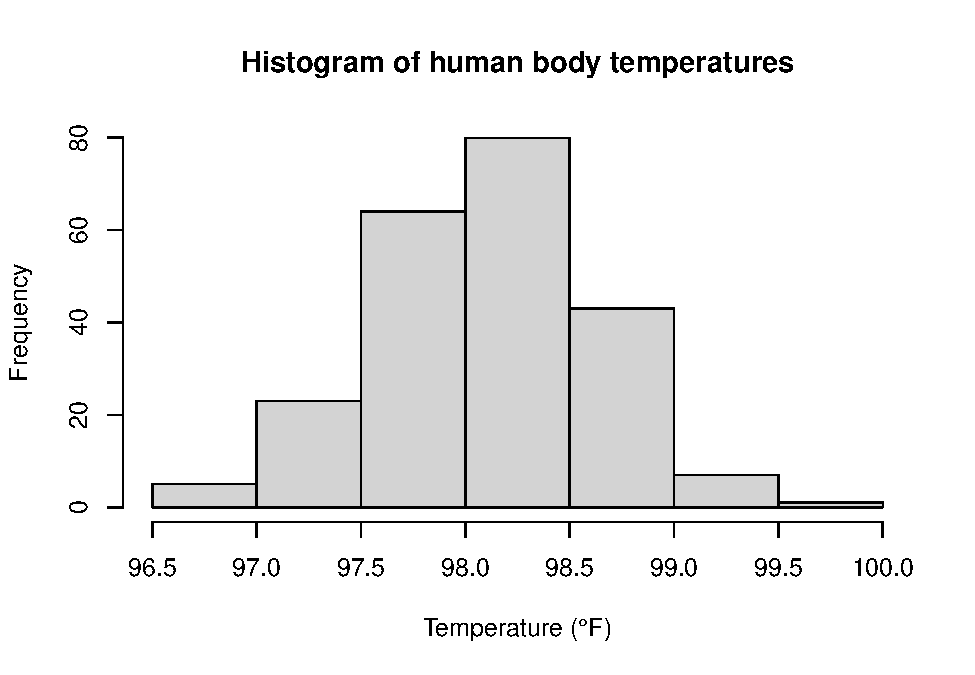
\includegraphics{6G4Z3008-notes_files/figure-latex/hist-1.pdf}

\begin{Shaded}
\begin{Highlighting}[]
\CommentTok{# These are the endpoints of the intervals}
\NormalTok{h}\OperatorTok{$}\NormalTok{breaks}
\end{Highlighting}
\end{Shaded}

\begin{verbatim}
## [1]  96.5  97.0  97.5  98.0  98.5  99.0  99.5 100.0
\end{verbatim}

\begin{Shaded}
\begin{Highlighting}[]
\CommentTok{# These are the observed frequencies}
\NormalTok{h}\OperatorTok{$}\NormalTok{counts }
\end{Highlighting}
\end{Shaded}

\begin{verbatim}
## [1]  5 23 64 80 43  7  1
\end{verbatim}

So we can summarise the histogram as a table:

\begin{longtable}[]{@{}cc@{}}
\toprule
Interval & Observed frequency\tabularnewline
\midrule
\endhead
\(96.5\leq x < 97\) & 5\tabularnewline
\(97\leq x < 97.5\) & 23\tabularnewline
\(97.5\leq x < 98\) & 64\tabularnewline
\(98\leq x < 98.5\) & 80\tabularnewline
\(98.5\leq x < 99\) & 43\tabularnewline
\(99\leq x < 99.5\) & 7\tabularnewline
\(99.5\leq x < 100\) & 1\tabularnewline
\bottomrule
\end{longtable}

Now this table is for the distribution of body temperatures in question. We want to compare this to a normal distribution, and one way of doing so is to standardise the intervals and work out the areas of the standard normal between the standardised endpoints.

\begin{Shaded}
\begin{Highlighting}[]
\CommentTok{#standardising the endpoints}
\NormalTok{st_breaks <-}\StringTok{ }\NormalTok{(h}\OperatorTok{$}\NormalTok{breaks }\OperatorTok{-}\StringTok{ }\NormalTok{xbar)}\OperatorTok{/}\NormalTok{sx}

\CommentTok{# creating a vector to store the probabilities in}
\NormalTok{probs <-}\StringTok{ }\KeywordTok{vector}\NormalTok{(}\DataTypeTok{length =} \KeywordTok{length}\NormalTok{(st_breaks)}\OperatorTok{-}\DecValTok{1}\NormalTok{)}

\CommentTok{# A loop to calculate the probability between endpoints}
\ControlFlowTok{for}\NormalTok{ (i }\ControlFlowTok{in} \DecValTok{1}\OperatorTok{:}\KeywordTok{length}\NormalTok{(probs))\{}
\NormalTok{probs[i] <-}\StringTok{ }\KeywordTok{pnorm}\NormalTok{(st_breaks[i}\OperatorTok{+}\DecValTok{1}\NormalTok{])}\OperatorTok{-}\KeywordTok{pnorm}\NormalTok{(st_breaks[i])}
\NormalTok{\}}


\CommentTok{#changing the end probabilities to account for the tails}
\CommentTok{#see comment below}
\NormalTok{probs[}\DecValTok{1}\NormalTok{] <-}\StringTok{ }\NormalTok{probs[}\DecValTok{1}\NormalTok{] }\OperatorTok{+}\StringTok{ }\KeywordTok{pnorm}\NormalTok{(st_breaks[}\DecValTok{1}\NormalTok{])}
\NormalTok{probs[}\KeywordTok{length}\NormalTok{(probs)] <-}\StringTok{  }\DecValTok{1} \OperatorTok{-}\StringTok{ }\KeywordTok{pnorm}\NormalTok{(st_breaks[}\KeywordTok{length}\NormalTok{(probs)])}

\NormalTok{probs}
\end{Highlighting}
\end{Shaded}

\begin{verbatim}
## [1] 0.013573730 0.090049579 0.273534295 0.360214167 0.205972393 0.050980284
## [7] 0.005675552
\end{verbatim}

However the intervals at either end must also account for the tail probabilities (just because the data ended there, does not mean that a smaller or larger value could not be observed in another sample, so it affects our expected calculation).

We get the following table of probabilities:

\begin{longtable}[]{@{}cc@{}}
\toprule
Interval & Probability\tabularnewline
\midrule
\endhead
\(96.5\leq x < 97\) & 0.01357\tabularnewline
\(97\leq x < 97.5\) & 0.09005\tabularnewline
\(97.5\leq x < 98\) & 0.27353\tabularnewline
\(98\leq x < 98.5\) & 0.36021\tabularnewline
\(98.5\leq x < 99\) & 0.20597\tabularnewline
\(99\leq x < 99.5\) & 0.05098\tabularnewline
\(99.5\leq x < 100\) & 0.00568\tabularnewline
\bottomrule
\end{longtable}

We then work out the expected numbers by multiplying by the total frequency:

\begin{Shaded}
\begin{Highlighting}[]
\NormalTok{E <-}\StringTok{ }\NormalTok{probs}\OperatorTok{*}\KeywordTok{sum}\NormalTok{(h}\OperatorTok{$}\NormalTok{counts)}
\NormalTok{E}
\end{Highlighting}
\end{Shaded}

\begin{verbatim}
## [1]  3.026942 20.081056 60.998148 80.327759 45.931844 11.368603  1.265648
\end{verbatim}

\begin{longtable}[]{@{}cc@{}}
\toprule
Probability & Expected\tabularnewline
\midrule
\endhead
0.01357 & 3.026\tabularnewline
0.09005 & 20.081\tabularnewline
0.27353 & 60.998\tabularnewline
0.36021 & 80.328\tabularnewline
0.20597 & 45.932\tabularnewline
0.05098 & 11.369\tabularnewline
0.01110 & 1.266\tabularnewline
\bottomrule
\end{longtable}

Then we combine the categories where the expected is less than \(5\). You may have to do this `manually':

\begin{Shaded}
\begin{Highlighting}[]
\NormalTok{E[}\DecValTok{2}\NormalTok{] <-}\StringTok{ }\NormalTok{E[}\DecValTok{1}\NormalTok{]}\OperatorTok{+}\NormalTok{E[}\DecValTok{2}\NormalTok{] }\CommentTok{#combine 1st and 2nd expected no.s}

\NormalTok{E[}\DecValTok{6}\NormalTok{] <-}\StringTok{ }\NormalTok{E[}\DecValTok{7}\NormalTok{]}\OperatorTok{+}\NormalTok{E[}\DecValTok{6}\NormalTok{] }\CommentTok{#combine 6th and last expected no.s}

\CommentTok{#Overwrite our E vector}
\NormalTok{E <-}\StringTok{ }\NormalTok{E[}\OperatorTok{-}\KeywordTok{c}\NormalTok{(}\DecValTok{1}\NormalTok{,}\DecValTok{7}\NormalTok{)] }\CommentTok{#get rid of 1st & last entries}
\NormalTok{E}
\end{Highlighting}
\end{Shaded}

\begin{verbatim}
## [1] 23.10800 60.99815 80.32776 45.93184 12.63425
\end{verbatim}

\begin{Shaded}
\begin{Highlighting}[]
\CommentTok{# Do the same for the observed frequencies:}
\NormalTok{O <-}\StringTok{ }\NormalTok{h}\OperatorTok{$}\NormalTok{counts}

\CommentTok{#same combining as for expected categories}
\NormalTok{O[}\DecValTok{2}\NormalTok{] <-}\StringTok{ }\NormalTok{O[}\DecValTok{1}\NormalTok{]}\OperatorTok{+}\NormalTok{O[}\DecValTok{2}\NormalTok{] }\CommentTok{#combine 1st and 2nd expected no.s}

\NormalTok{O[}\DecValTok{6}\NormalTok{] <-}\StringTok{ }\NormalTok{O[}\DecValTok{7}\NormalTok{]}\OperatorTok{+}\NormalTok{O[}\DecValTok{6}\NormalTok{] }\CommentTok{#combine 6th and last expected no.s}

\CommentTok{#Overwrite our E vector}
\NormalTok{O <-}\StringTok{ }\NormalTok{O[}\OperatorTok{-}\KeywordTok{c}\NormalTok{(}\DecValTok{1}\NormalTok{,}\DecValTok{7}\NormalTok{)] }\CommentTok{#get rid of 1st & last entries}
\NormalTok{O}
\end{Highlighting}
\end{Shaded}

\begin{verbatim}
## [1] 28 64 80 43  8
\end{verbatim}

Now we redraw the combined table with the observed numbers to calculate the test statistic \(X^2\).

\begin{longtable}[]{@{}cc@{}}
\toprule
0 & E\tabularnewline
\midrule
\endhead
28 & 23.108\tabularnewline
64 & 60.998\tabularnewline
80 & 80.328\tabularnewline
43 & 45.932\tabularnewline
8 & 12.634\tabularnewline
\bottomrule
\end{longtable}

We can do this calculation using vectors in R. You may also find using a spreadsheet helps.

\begin{Shaded}
\begin{Highlighting}[]
\NormalTok{X_sq <-}\StringTok{ }\KeywordTok{sum}\NormalTok{((O}\OperatorTok{-}\NormalTok{E)}\OperatorTok{^}\DecValTok{2}\OperatorTok{/}\NormalTok{E) }
\NormalTok{X_sq}
\end{Highlighting}
\end{Shaded}

\begin{verbatim}
## [1] 3.071697
\end{verbatim}

\begin{Shaded}
\begin{Highlighting}[]
\KeywordTok{qchisq}\NormalTok{(}\FloatTok{0.95}\NormalTok{,}\DataTypeTok{df =}\DecValTok{2}\NormalTok{)}
\end{Highlighting}
\end{Shaded}

\begin{verbatim}
## [1] 5.991465
\end{verbatim}

Here there are \(5\) categories after combining, and we estimated \(2\) parameters, so the degrees of freedom are given by \(\nu = 5-1-2=2\).
Here the critical value is \(5.991465\). The test statistic has value 3.071697, so here we do not reject \(\text{H}_0\) and conclude that the data is consistent with a \(\text{N}(98.2,0.527^2)\) distribution.

Note if we combine the categories in the probability vector then R can do our test quickly as:

\begin{Shaded}
\begin{Highlighting}[]
\CommentTok{#same combining as for probability categories}
\NormalTok{probs[}\DecValTok{2}\NormalTok{] <-}\StringTok{ }\NormalTok{probs[}\DecValTok{1}\NormalTok{]}\OperatorTok{+}\NormalTok{probs[}\DecValTok{2}\NormalTok{] }\CommentTok{#combine 1st and 2nd expected no.s}

\NormalTok{probs[}\DecValTok{6}\NormalTok{] <-}\StringTok{ }\NormalTok{probs[}\DecValTok{7}\NormalTok{]}\OperatorTok{+}\NormalTok{probs[}\DecValTok{6}\NormalTok{] }\CommentTok{#combine 6th and last expected no.s}

\CommentTok{#Overwrite our E vector}
\NormalTok{probs <-}\StringTok{ }\NormalTok{probs[}\OperatorTok{-}\KeywordTok{c}\NormalTok{(}\DecValTok{1}\NormalTok{,}\DecValTok{7}\NormalTok{)] }\CommentTok{#get rid of 1st & last entries}
\NormalTok{probs}
\end{Highlighting}
\end{Shaded}

\begin{verbatim}
## [1] 0.10362331 0.27353429 0.36021417 0.20597239 0.05665584
\end{verbatim}

\begin{Shaded}
\begin{Highlighting}[]
\KeywordTok{chisq.test}\NormalTok{(}\DataTypeTok{x =}\NormalTok{ O, }\DataTypeTok{p =}\NormalTok{ probs)}
\end{Highlighting}
\end{Shaded}

\begin{verbatim}
## 
##  Chi-squared test for given probabilities
## 
## data:  O
## X-squared = 3.0717, df = 4, p-value = 0.5459
\end{verbatim}

This is a good check of our test statistic, however R does not know we combined the categories so the df are incorrect and so is the p-value.

\hypertarget{explanation-of-statistic-x2-non-examinable}{%
\section{\texorpdfstring{Explanation of Statistic \(X^2\) (non-examinable)}{Explanation of Statistic X\^{}2 (non-examinable)}}\label{explanation-of-statistic-x2-non-examinable}}

This section aims to give some intuition for the question: why is the statistic \(X^2 = \sum_{i=1}^m \frac{(O_i-E_i)^2}{E_i}\) a \(\chi^2\) distribution?

Suppose in the simplest case we have just two outcomes to observe rather than many so we have a binomial distribution \(Y_1 \sim \text{Bin}(n,\pi_1)\) and \(Y_2 = n - Y_1\). Also \(\pi_2 = 1-\pi_1\).

The observed numbers of the two outcomes are \(Y_1\) and \(Y_2\), and their expected numbers are \(n\pi_1\) and \(n\pi_2\). We consider the quantity:

\[X^2 = \frac{(Y_1-n\pi_1)^2}{n\pi_1} + \frac{(Y_2-n\pi_2)^2}{n\pi_2}\]
Using \(Y_2 = n - Y_1\) and \(\pi_2 = 1-\pi_1\) gives:

\[= \frac{(Y_1-n\pi_1)^2}{n\pi_1} + \frac{(n-Y_1-n(1-\pi_1))^2}{n(1-\pi_1)}\]

\[=\frac{(Y_1-n\pi_1)^2}{n\pi_1} + \frac{(Y_1-n\pi_1)^2}{n(1-\pi_1)}\]
Collecting as a single fraction:
\[=\frac{(Y_1-n\pi_1)^2(1-\pi_1)+(Y_1-n\pi_1)^2\pi_1}{n\pi_1(1-\pi_1)}\]
\[=\frac{(Y_1-n\pi_1)^2}{n\pi_1(1-\pi_1)}\]
Now we have

\[X^2 = \left( \frac{Y_1 - n\pi_1}{\sqrt{n\pi_1(1-\pi_1)}}\right)^2\]
Recall for a binomial distribution that the mean is \(n\pi\) and the variance is \(n\pi(1-\pi)\). Here this means that inside the brackets we have a standardised distribution - that is, we have subtracted the mean and divided by the standard deviation. By the Normal approximation to the binomial distribution, we know that this will be approximately a normal distribution, but because it is standardised it will be \(\text{N}(0,1)\).

Also recall that the square of a standard normal \(Z^2 \sim \chi^2_1\). Therefore we have

\[X^2 = Z^2 \sim \chi^2_1\]
When we had \emph{two} outcomes and the statistic \(X^2\) followed a \(\chi^2_1\) distribution. For a distribution with \(k\) categories, when there are \(k\) outcomes, \(X^2\) will follow a \(\chi^2_{k-1}\) distribution.

\hypertarget{summary-2}{%
\section{Summary}\label{summary-2}}

\hypertarget{goodness-of-fit-tests}{%
\subsection{Goodness of fit tests}\label{goodness-of-fit-tests}}

\begin{itemize}
\item
  A chi-squared test is always a right tailed test
\item
  The null hypothesis is always that the distribution is a good fit
\item
  Work out expected numbers by multiplying the probability by the total frequency.
\end{itemize}

\[E = \text{total}\times \text{P}(X=x)\]

\begin{itemize}
\item
  you have to combine categories where the expected numbers are less than \(5\).
\item
  The number of degrees of freedom \(\nu = \text{no. categories after combining} - 1\)
\item
  If you have to estimate a parameter you need to subtract one from the degrees of freedom.
\end{itemize}

\[\nu = \text{no. categories after combining} - 1 - \text{no. parameters estimated}\]

\hypertarget{contingency-tables}{%
\subsection{Contingency tables}\label{contingency-tables}}

\begin{itemize}
\item
  Here the null hypothesis is that there is no association.
\item
  The degrees of freedom is the one less than the number of columns multiplied by one less than the number of rows, after combining classes where \(E<5\).
  \[\nu =  (c-1)(r-1)\]
\item
  To work out the expected you multiply row and column totals and divide by the grand total.
\end{itemize}

\hypertarget{exercises-week-9}{%
\section{Exercises Week 9}\label{exercises-week-9}}

\begin{exercise}
A tetrahedral die is thrown \(120\) times and the number on which it lands is noted

\begin{longtable}[]{@{}ccccc@{}}
\toprule
Number & 1 & 2 & 3 & 4\tabularnewline
\midrule
\endhead
Frequency & 35 & 32 & 25 & 28\tabularnewline
\bottomrule
\end{longtable}

Test at the \(5\%\) significance level whether the die is fair.
\end{exercise}

\begin{exercise}

A new Fly spray is applied to \(50\) samples each of five flies in an air-tight box, and the number of living flies is counted after one hour. The results were:

\begin{longtable}[]{@{}ccccccc@{}}
\toprule
Number & 0 & 1 & 2 & 3 & 4 & 5\tabularnewline
\midrule
\endhead
Frequency & 7 & 20 & 12 & 9 & 1 & 1\tabularnewline
\bottomrule
\end{longtable}

\begin{enumerate}
\def\labelenumi{\alph{enumi})}
\item
  Under what circumstances would you expect to be able to model a variable \(X\) with a binomial distribution?
\item
  i)What is the mean of a Binomial distribution if it has parameters \(n\) and \(p\)?

  \begin{enumerate}
  \def\labelenumii{\roman{enumii})}
  \setcounter{enumii}{1}
  \tightlist
  \item
    Calculate the mean number of living flies per sample.
  \end{enumerate}
\item
  Calculate the expected values and perform a \(\chi^2\) test at the \(5\%\) significance level.
\end{enumerate}

\end{exercise}

\begin{exercise}

A group of students are performing an experiment where they drop \(20\) drawing pins on the ground and the number landing pointing down is counted. The experiment was carried out until the students had \(50\) observations. The results are in the table:

\begin{longtable}[]{@{}cc@{}}
\toprule
Number landing down & Frequency\tabularnewline
\midrule
\endhead
3 & 2\tabularnewline
4 & 2\tabularnewline
5 & 5\tabularnewline
6 & 7\tabularnewline
7 & 17\tabularnewline
8 & 8\tabularnewline
9 & 6\tabularnewline
10 & 1\tabularnewline
11 & 2\tabularnewline
\bottomrule
\end{longtable}

\begin{enumerate}
\def\labelenumi{\alph{enumi})}
\item
  Calculate the mean number landing point down. Hence show an estimate for the probability of a pin landing facing down is \(0.35\)
\item
  What are the parameters of the appropriate binomial distribution for this data? Calculate the probability of exactly \(8\) landing point down, and hence work out its expected frequency.
\item
  Calculate the expected number of times five or fewer pins would land point down.
\item
  The goodness of fit test is partially complete below. By grouping the data appropriately, evaluate the missing expected or observed frequencies. Hence calculate the value of \(X^2\) for this data.
\end{enumerate}

\begin{longtable}[]{@{}cccccc@{}}
\toprule
Number of pins & \(\leq 5\) & 6 & 7 & 8 & \(\geq 9\)\tabularnewline
\midrule
\endhead
Expected & & 8.6 & & & 11.8\tabularnewline
Observed & 9 & 7 & 17 & &\tabularnewline
\bottomrule
\end{longtable}

\begin{enumerate}
\def\labelenumi{\alph{enumi})}
\setcounter{enumi}{4}
\tightlist
\item
  How many degrees of freedom does the test have? Carry out the test making your findings clear.
\end{enumerate}

\end{exercise}

\begin{exercise}

A local council has a record of the number of children and the number of households in its area. The council calculates the average number of children per household is \(1.4\). It is suggested that the number of children per household may be modelled by a Poisson distribution with parameter \(1.4\). In order to test this a random sample of \(1000\) households is taken, giving the following data.

\begin{longtable}[]{@{}ccccccc@{}}
\toprule
Number of children & 0 & 1 & 2 & 3 & 4 & \(\geq 5\)\tabularnewline
\midrule
\endhead
Number of households & 273 & 361 & 263 & 78 & 21 & 4\tabularnewline
\bottomrule
\end{longtable}

\begin{enumerate}
\def\labelenumi{\alph{enumi})}
\item
  Calculate the corresponding expected frequencies obtained from the Poisson distribution with parameter \(1.4\).
\item
  Carry out a \(5\%\) significance test to show the proposed model should not be accepted.
\item
  With reference to relevant figures, give a reason in context for the lack of fit to the proposed model.
\item
  Which of the assumptions of a Poisson model may not be valid in this example?
\end{enumerate}

\end{exercise}

\begin{exercise}

The number of heavy rainstorms reported by \(330\) weather stations in the US over a one-year period are as follows:

\begin{longtable}[]{@{}cc@{}}
\toprule
Number of rainstorms (x) & Number of stations (f)\tabularnewline
\midrule
\endhead
0 & 102\tabularnewline
1 & 114\tabularnewline
2 & 74\tabularnewline
3 & 28\tabularnewline
4 & 10\tabularnewline
5 & 2\tabularnewline
\(> 5\) & 0\tabularnewline
\bottomrule
\end{longtable}

\begin{enumerate}
\def\labelenumi{\alph{enumi})}
\item
  Find the expected frequencies of rainstorms given by the Poisson distribution having the same mean and total as the observed data.
\item
  Carry out a \(\chi^2\) test for the adequacy of the Poisson distribution as a model for these data.
\end{enumerate}

\end{exercise}

\begin{exercise}
A farmer's cooperative decided to test three new fertilisers A, B and C. They allocated them at random to \(75\) plots. The yield of the crop was then classified as high, medium or low. The results are summarised below:

\begin{longtable}[]{@{}ccccc@{}}
\toprule
& A & B & C & Total\tabularnewline
\midrule
\endhead
High & 12 & 15 & 3 & 30\tabularnewline
Medium & 8 & 8 & 8 & 24\tabularnewline
Low & 5 & 7 & 9 & 21\tabularnewline
Total & 25 & 30 & 20 & 75\tabularnewline
\bottomrule
\end{longtable}

Test at the \(5\%\) level of significance whether there is any evidence of an association between brand of fertiliser and crop yield.
\end{exercise}

\begin{exercise}
A survey of the effectiveness of three hospitals A, B and C in treating a particular illness revealed the following:

\begin{longtable}[]{@{}cccc@{}}
\toprule
& Complete recovery & Partial recovery & Died\tabularnewline
\midrule
\endhead
A & 37 & 23 & 7\tabularnewline
B & 52 & 44 & 12\tabularnewline
C & 22 & 30 & 13\tabularnewline
\bottomrule
\end{longtable}

Do the data reveal significant evidence of differences in the effectiveness of the hospitals?
\end{exercise}

\hypertarget{linear-modelling-and-correlation}{%
\chapter{Linear modelling and correlation}\label{linear-modelling-and-correlation}}

In this final week we will be learning about linear modelling via regression and correlation. The aims are to understand the linear regression model and identify the response and regressor variables, use the model for prediction and the potential limitations of the model. Further we will analyse residuals and identify problems with the model from this viewpoint.

Next we will understand the concept of a correlation coefficient and some potential pitfalls in their use and interpretation.

\hypertarget{linear-regression}{%
\section{Linear regression}\label{linear-regression}}

Regression is concerned with modelling the relationship between two (or more) variables. We have concentrated principally on developing methods for a single random variable, but many data sets provide information about several variables and we want to study connections between these variables. We will concentrate on quantitative variables \(x\) and \(y\) where these are observed in pairs \((x,y)\).

The data may be collected at the same time. Some examples:

\begin{longtable}[]{@{}cc@{}}
\toprule
\(x\) & \(y\)\tabularnewline
\midrule
\endhead
Speed of ski jumper & Distance jumped\tabularnewline
Hand span & Foot length\tabularnewline
No.~red blood cells & No.~white blood cells\tabularnewline
Size of house & Value of house\tabularnewline
\bottomrule
\end{longtable}

However the data may be collected at a later time though the link is clear. We will not study the temporal aspect here.

\begin{longtable}[]{@{}cc@{}}
\toprule
\(x\) & \(y\)\tabularnewline
\midrule
\endhead
Mark in a mock exam & Mark in real exam\tabularnewline
Amount of fertiliser & Amount of growth\tabularnewline
Height of father & Height of adult son\tabularnewline
\bottomrule
\end{longtable}

In some cases the variable \(x\) affects the variable \(y\). In other cases both may be affected by some third unmeasured factor.

\begin{definition}
The variable \(x\) is called the \emph{explanatory} or \emph{independent} variable. The variable \(y\) is called the \emph{response} or \emph{dependent} variable.
\end{definition}

\begin{example}
The petrol consumption of a car is related to the speed at which it is driven.

\begin{longtable}[]{@{}ccccccccc@{}}
\toprule
mph & 35 & 35 & 35 & 35 & 40 & 40 & 40 & 40\tabularnewline
\midrule
\endhead
mpg & 48.4 & 47.6 & 47.8 & 46.2 & 45.8 & 45.6 & 45.0 & 44.9\tabularnewline
\bottomrule
\end{longtable}

\begin{longtable}[]{@{}ccccccccc@{}}
\toprule
mph & 45 & 45 & 45 & 45 & 50 & 50 & 50 & 50\tabularnewline
\midrule
\endhead
mpg & 43.0 & 42.8 & 42.7 & 42.2 & 39.9 & 40.3 & 38.9 & 39.6\tabularnewline
\bottomrule
\end{longtable}

Suggest the likely average fuel consumption of a car travelling at 42 mph.
\end{example}

Here is a similar example with the fuel consumption and weight of car.

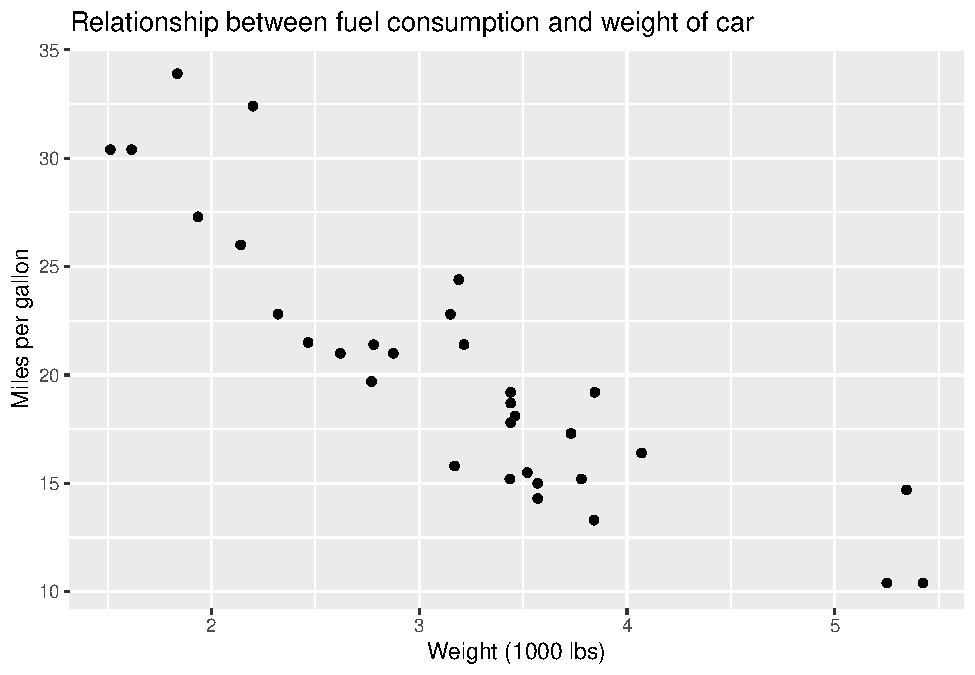
\includegraphics{6G4Z3008-notes_files/figure-latex/fuel1-1.pdf}

Here is another example from a political context.

\begin{figure}

{\centering 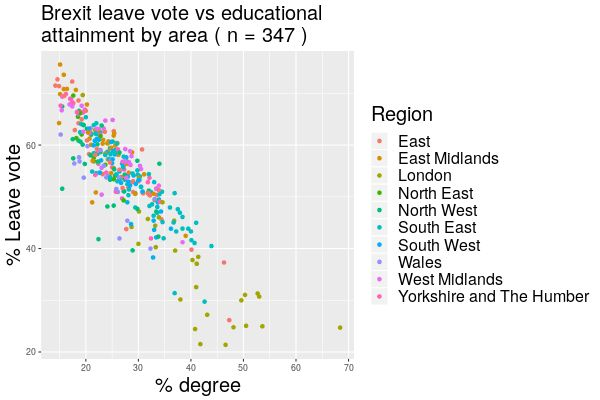
\includegraphics[width=0.75\linewidth]{./figures/Brexit} 

}

\caption{Regions with a lower percentage of graduates had a higher proportion of those voting leave}\label{fig:brexit}
\end{figure}

The simplest relationship to consider between \(y\) and \(x\) is the straight line \(y=a+bx\). When points are plotted we are often in a situation where the points do not lie exactly on any straight line.

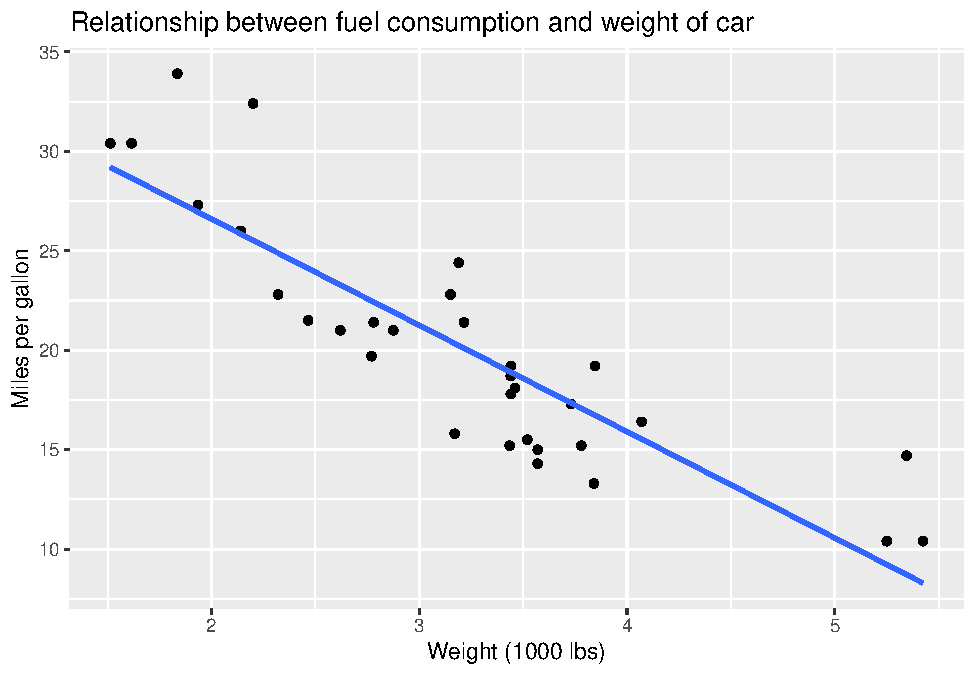
\includegraphics{6G4Z3008-notes_files/figure-latex/fuel2-1.pdf}

One needs to account for some error in the observation.

\begin{definition}
The \emph{simple linear regression model} is the equation
\[Y=a+bX+\varepsilon\]

where \(\varepsilon\) is a normally distributed random variable with mean zero and some constant variance. That is,

\[\varepsilon \sim \text{N}(0,\sigma^2)\]
For any particular value \(X=x_i\) and \(Y = y_i\), we would predict \(a+bx_i\). Sometimes the model is summarised as \(\text{E}(Y)=a+bX\).

The \emph{regression line} is the line
\[y = a +bx\]
\end{definition}

To fit the model \(y=a+bx\) the points could be plotted and \(a\) and \(b\) estimated by eye. However this is a subjective process. For two independent variables it becomes difficult to fit by eye, and in higher dimensions this is impossible to do. We consider what constrains line.

\begin{definition}
Given an observed datum \((x_i,y_i)\) and a fitted regression line \(y=a+bx\), the \textbf{\emph{residual}} \(r_i\) is the difference between the observed value and the value predicted by the regression line. That is,

\[r_i = y_i - (a+bx_i)\]
\end{definition}

Small residuals are desirable. However, residuals can be positive or negative, depending on whether the point lies vertically above or below the regression line. Taken together, we see that minimising the sum of squared residuals will achieve the optimal linear model. That is, if we let
\[S = \sum_{i=1}^{n}r_i^2\]
Then \emph{the} regression line \(y=a+bx\) minimises \(S\).

\begin{verbatim}
## Warning: The `<scale>` argument of `guides()` cannot be `FALSE`. Use "none" instead as
## of ggplot2 3.3.4.
## This warning is displayed once every 8 hours.
## Call `lifecycle::last_lifecycle_warnings()` to see where this warning was
## generated.
\end{verbatim}

\begin{figure}
\centering
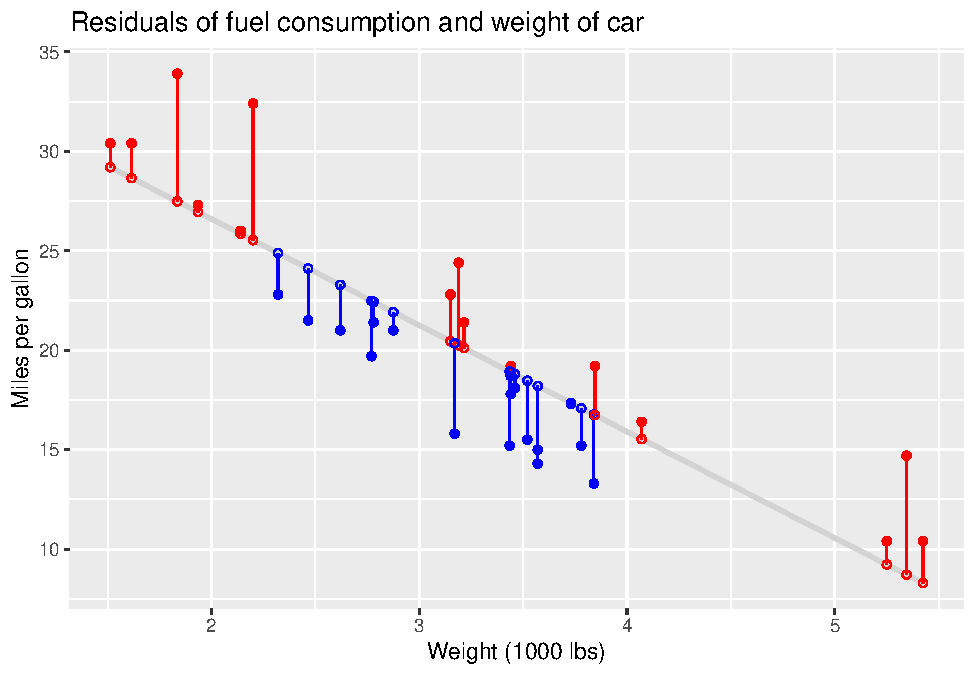
\includegraphics{6G4Z3008-notes_files/figure-latex/resids1-1.pdf}
\caption{\label{fig:resids1}Red residuals are positive, and blue residuals are negative}
\end{figure}

\begin{theorem}
Given \(n\) points \((x_i,y_i)\), \(1\leq i\leq n\), and regression line \(y=a+bx\) then we have that

\[a = \bar{y}-b\bar{x},\]
\[b = \frac{s_{xy}}{s_{xx}},\]
where
\[s_{xx} = \sum x_i^2 - \frac{(\sum x_i )^2}{n}\]
and
\[s_{xy} = \sum x_iy_i - \frac{(\sum x_i )(\sum y_i )}{n} \]
\end{theorem}

\emph{proof}

Consider the sum of the squared residuals

\[S = \sum_{i=1}^{n} r_i^2\]

Then \(S=S(a,b)\) is a function of \(a\) and \(b\).

\[S(a,b)=\sum_{i=1}^{n} (y_i - (a+bx_i))^2\]
Expanding gives

\[S(a,b) = \sum y_i^2 - 2a\sum y_i - 2b\sum x_i y_i + a^2n + 2ab\sum x_i + b^2 \sum x_i^2\]

Now we can find the minumum of this function (which is a minimum because it is a sum of squares) by partially differentiating and setting this equal to zero.

\[\frac{\partial S(a,b)}{\partial a} =-2\sum y_i+ 2an +2b\sum x_i\]
Setting \(\frac{\partial S(a,b)}{\partial a}=0\) implies,

\[0=-\sum y_i+ an +b\sum x_i \]

\[a= \frac{1}{n}\left(\sum y_i - b \sum x_i\right).\]
Likewise partially differentiating with respect to \(b\) gives:
\[ \frac{\partial S(a,b)}{\partial b} = -2\sum x_i y_i+2a\sum x_i + 2b\sum x_i^2\]
Again setting this equal to zero gives:

\[= -\sum x_i y_i+a\sum x_i + b\sum x_i^2 ,\]
which implies

\[b = \frac{\sum x_iy_i - a\sum x_i}{\sum x_i^2}.\]
Substituting in the result for \(a\) gives the result.

\begin{example}
Fit a linear regression line to the following data

\begin{longtable}[]{@{}ccccc@{}}
\toprule
\(x\) & 2 & 3 & 5 & 7\tabularnewline
\midrule
\endhead
\(y\) & 4 & 7 & 9 & 12\tabularnewline
\bottomrule
\end{longtable}

\emph{solution}

\begin{longtable}[]{@{}cccc@{}}
\toprule
\(y\) & \(x\) & \(xy\) & \(x^2\)\tabularnewline
\midrule
\endhead
4 & 2 & 8 & 4\tabularnewline
7 & 3 & 21 & 9\tabularnewline
9 & 5 & 45 & 25\tabularnewline
12 & 7 & 84 & 49\tabularnewline
\(\sum y =32\) & \(\sum x = 17\) & \(\sum xy = 158\) & \(\sum x^2 = 87\)\tabularnewline
\bottomrule
\end{longtable}

Then

\[b = \frac{\sum xy - \frac{\sum x \sum y}{n}}{\sum x^2 - \frac{(\sum x)^2}{n}} \]
\[=\frac{158 - \frac{17\times32}{4}}{87 - \frac{17^2}{4}} =1.4915\]

and

\[a = \frac{1}{n}(\sum y -b \sum x) =\frac{1}{4}(32 - 1.4915\times 17) = 1.661\]
So the line is

\[y = 1.66 + 1.49x\]
\end{example}

\begin{example}
For the car data in example \(10.1\). We have that \(n=16\) and the following:
\[\sum x_i = 680 \ , \ \sum x_i^2 = 29400\]
\[\sum y_i = 700.7 \ , \ \sum y_i^2 = 30828.05\]
Calculate the least squares estimates of \(a\) and \(b\).

\emph{answer}

\[s_{xy} = 29518.5 - \left(\frac{680\times700.7}{16}\right) = -261.25\]
\[s_{xx} = 29400 - \left(\frac{680^2}{16}\right) = 500.00\]
\[b = \frac{s_{xy}}{s_{xx}} = \frac{-261.25}{500.00}= -0.5225\]
\[a= \bar{y}-b\bar{x}=\frac{1}{16}[700.7 - (0.5225\times680)]= 66.0\]
Hence the line is
\[y = 66.0 -0.5225x\]
And the predicted value at \(42\)mph is therefore
\[y = 66.0 -0.5225\times 42 = 44.055\approx 44\]
\end{example}

A linear model can be fitted in R with the command \(\texttt{lm(formula = y}\sim\texttt{x)}\).

\hypertarget{residual-analysis}{%
\section{Residual analysis}\label{residual-analysis}}

The residuals are realisations of the modelled error term \(\varepsilon \sim \text{N}(0,\sigma^2)\). If the model is appropriate then we would expect the residuals to look approximately as if from this normal distribution. That is, they should be small in magnitude and random. This can be investigated graphically.

\begin{example}
The residuals in the earlier example can be plotted in a histogram, and we can plot a quantile-quantile plot, and series plots.

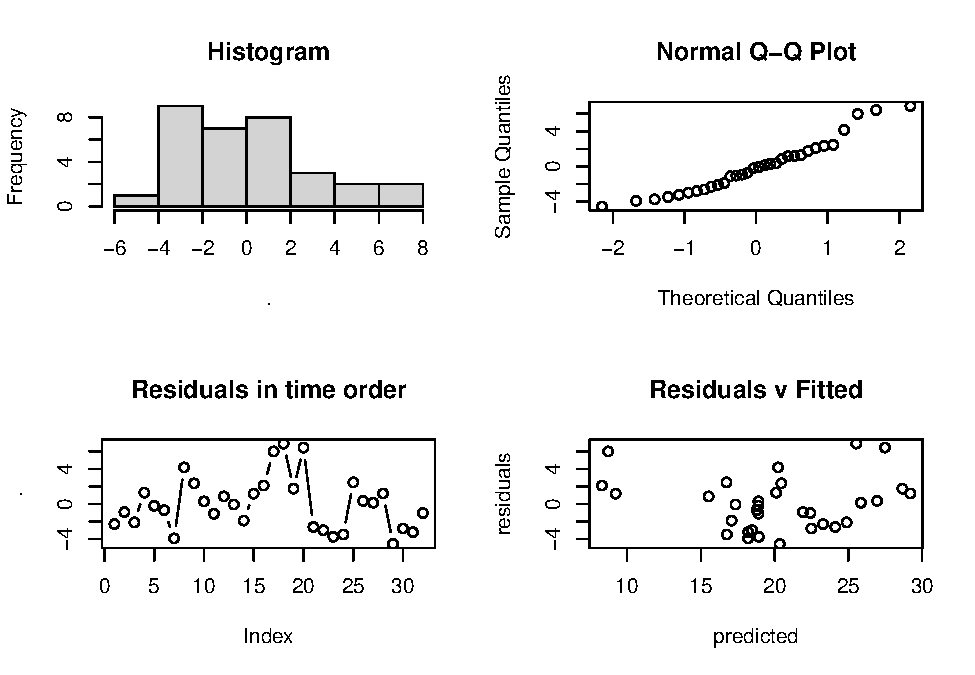
\includegraphics{6G4Z3008-notes_files/figure-latex/residplots-1.pdf}
\end{example}

In general, the following may be noted about these plots.

\begin{itemize}
\item
  The quantile-quantile plot matches the observed sample quantile with the quantiles of the theoretical normal distribution, and so for a good fit one would expect a straight line with gradient \(1\).
\item
  Residuals series, there should be no consistent pattern over time (i.e.~regular increase or decrease) and there should be no outliers.
\item
  The histogram should look unimodal and symmetrical.
\item
  residual and fitted value scatter plot should have no evident patterns.
\end{itemize}

Let's see an example where this does not work.

\begin{example}
In an experiment into using a biological enzyme in washing powder the enzyme activity \(y\) was measured at different washing temperatures \(x\).

\begin{longtable}[]{@{}ccccccccccc@{}}
\toprule
x & 20 & 30 & 40 & 50 & 60 & 70 & 80 & 90 & &\tabularnewline
\midrule
\endhead
y & 162 & 207 & 234 & 240 & & & & & &\tabularnewline
\bottomrule
\end{longtable}

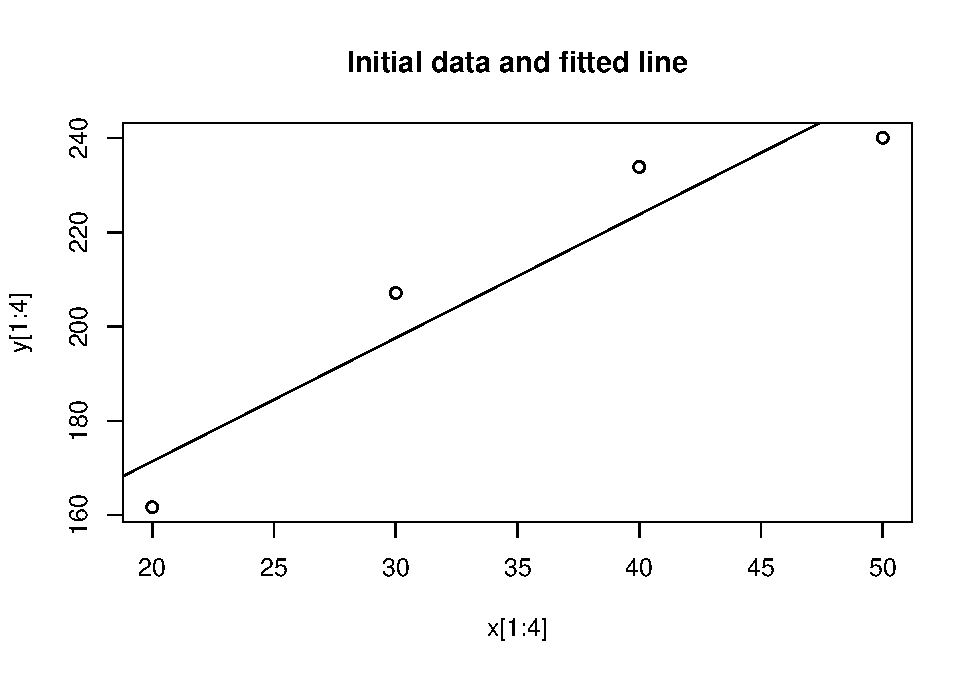
\includegraphics{6G4Z3008-notes_files/figure-latex/enzyme1-1.pdf}

Further data is collected:

\begin{longtable}[]{@{}ccccccccccc@{}}
\toprule
x & 20 & 30 & 40 & 50 & 60 & 70 & 80 & 90 & &\tabularnewline
\midrule
\endhead
y & 162 & 207 & 234 & 240 & 233 & 217 & 189 & 154 & &\tabularnewline
\bottomrule
\end{longtable}

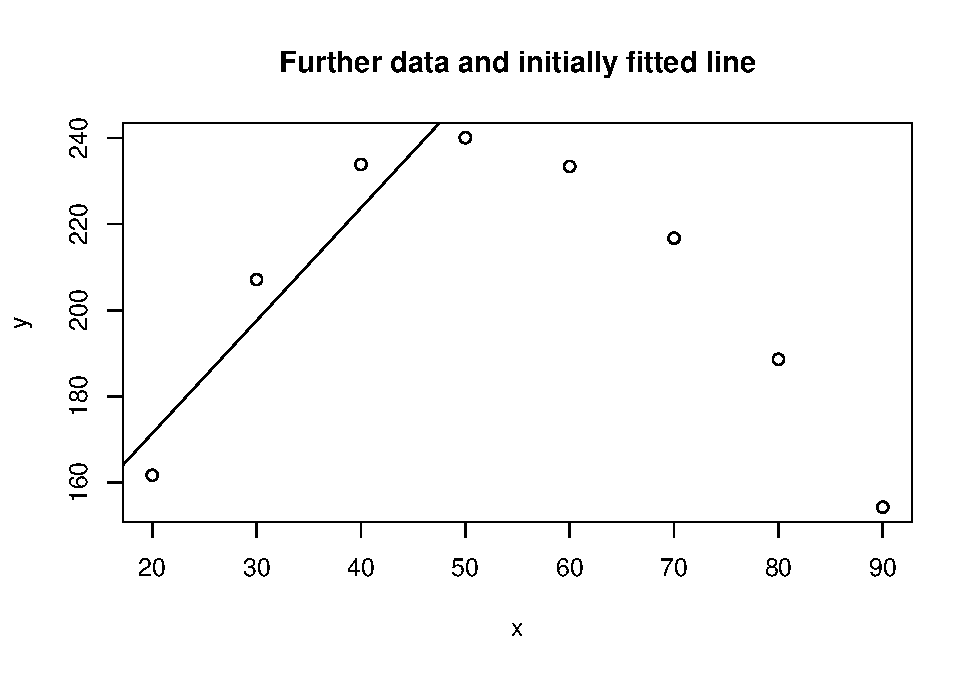
\includegraphics{6G4Z3008-notes_files/figure-latex/enzyme2-1.pdf}

Should a new line be fitted to the data?
\end{example}

If we look at the residuals from the original line over time we see that they are increasingly negative. This suggests that a linear is not suitable as a model, and a non-linear model such as a quadratic is more suitable. In context this may be because at higher temperatures the enzyme is denatured so is increasingly less effective.

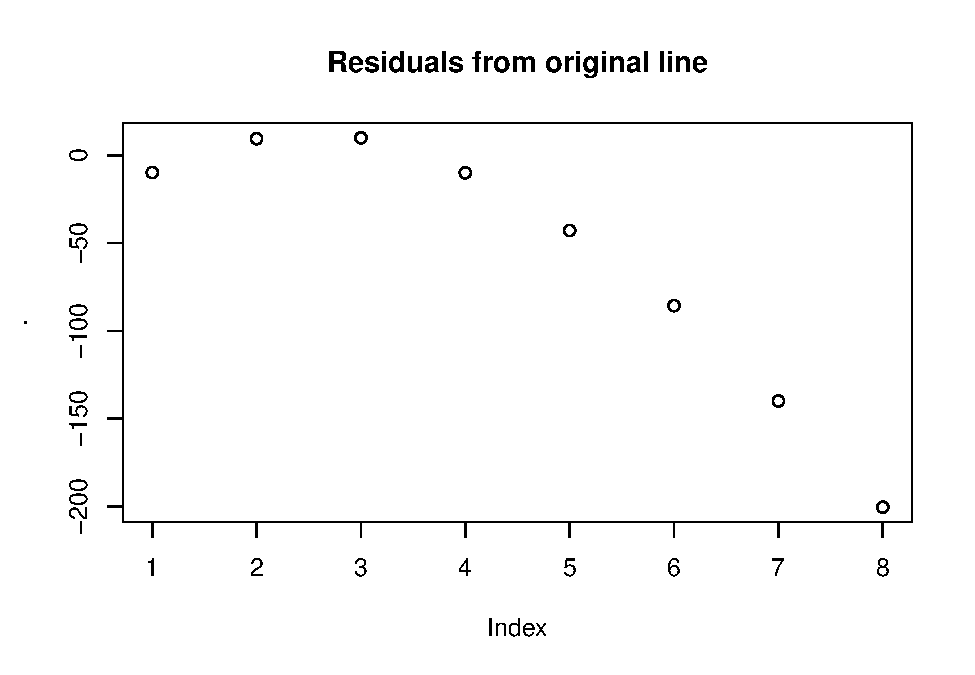
\includegraphics{6G4Z3008-notes_files/figure-latex/enzyme-1.pdf}

\hypertarget{analysis-of-variance}{%
\section{Analysis of Variance}\label{analysis-of-variance}}

The aim of fitting a regression model is to try and explain the variation in the response \(Y\) assuming it was generated by a linear model with random error.

\[y= a+bx+\varepsilon\]

Anything left over is random variation. A useful model will explain a significant proportion of this random variation. Thus,

\[\text{Variation in data} = \text{ variation in model} \  + \ \text{unexplained variation}\]
In linear models this variation is measured by sums of squares (SS) as follows:

\[SS_{T} =  SS_R + SS_E\]
So the total sum of squares equals the sum of squares due to regression add the error sum of squares.

The analysis is usually set out in an ANOVA table which can be used to test for the significance of the slope parameter.

\[H_0 : b=0\]
:::\{.definition\}
- The \textbf{\emph{total sum of squares}} is given by

\[SS_T = \sum (y-\bar{y})^2= \sum y^2 - \frac{(\sum y)^2}{n}\]
- The \textbf{\emph{regression sum of squares}} is given by

\[SS_R = b^2\sum(x-\bar{x})^2 = b^2 \left\{ \sum x^2 - \frac{(\sum x)^2}{n}\right\}\]
- The \textbf{\emph{error sum of squares}} is given by
\[SS_E=SS_T-SS_R \]
:::

\begin{definition}
The regression Analysis of Variance table is written as

\begin{longtable}[]{@{}cccc@{}}
\toprule
Source & Degrees of Freedom & SS & MS\tabularnewline
\midrule
\endhead
Regression & 1 & \(SS_R\) & \$SS\_R / 1 \$\tabularnewline
Error & \(n-2\) & \(SS_E\) & \(SS_E / (n-2)\)\tabularnewline
Total & \(n-1\) & \(SS_T\) &\tabularnewline
\bottomrule
\end{longtable}

This is given in the formula book. To test \(H_0 : b = 0\), one compares the ratio of the Mean sum of squares (MS) to the F-distribution critical value. That is,

\[F=\frac{MS_R}{MS_E}\sim F_{1,n-2} \]
\end{definition}

\begin{example}
Sales of major appliances vary with the new housing market. When new home sales are high, so too are the sales of appliances such as dishwashers, washing machines, and so on.

\begin{longtable}[]{@{}cc@{}}
\toprule
Housing starts (thousands) & Appliance sales (thousands)\tabularnewline
\midrule
\endhead
2.0 & 5.0\tabularnewline
2.5 & 5.5\tabularnewline
3.2 & 6.0\tabularnewline
3.6 & 7.0\tabularnewline
3.3 & 7.2\tabularnewline
4.0 & 7.7\tabularnewline
\bottomrule
\end{longtable}

Suppose we have calculated the regression line \(y=2.1549 + 1.3694x\) and the summary statistics:

\[\sum x = 18.6 \ , \ \sum x^2 = 60.34\]
\[\sum y = 38.4 \ , \ \sum y^2 = 251.38\]
Calculate the ANOVA table and test the hypothesis that \(H_0 : b = 0\).
\end{example}

\emph{solution}

We will only round at the end as we need to maintain accuracy to compare to a critical value.
\[SS_T = 251.38 - \frac{38.4^2}{6} = 5.62\]
\[SS_R = (1.3694)^2 \left( 60.34 - \frac{18.6^2}{6} \right) = 5.025\ldots\]
\[SS_E = SS_T - SS_R = 5.62 - 5.025\ldots = 0.5943\ldots \]

\[MS_R = 5.02\ldots /1 = 5.025 \]
\[MS_E = 0.5843\ldots / 4 = 0.1485\ldots\]

We can complete the ANOVA table as follows

\begin{longtable}[]{@{}cccc@{}}
\toprule
Source & Degrees of Freedom & SS & MS\tabularnewline
\midrule
\endhead
Regression & 1 & \(5.025687\) & \(5.025687\)\tabularnewline
Error & \(4\) & \(0.5943129\) & \(0.1485782\)\tabularnewline
Total & \(5\) & \(5.62\) &\tabularnewline
\bottomrule
\end{longtable}

We have that

\[F = \frac{5.025687}{0.1485782}=33.825188\]

From tables one can find the \(95^{\text{th}}\) percentile as \(F_{1,4}=7.71\)

Since \(33.83 > 7.71\) we can reject \(H_0\).

We can evaluate these tables manually, and may be required to do so in an exam, but they can be obtained from statistical software too, such as R. In R an ANOVA table can be obtained from the combination of the commands \(\texttt{aov()}\) and \(\texttt{summary()}\).

\begin{example}

In the housing example above we can do this analysis in R as follows:

\begin{Shaded}
\begin{Highlighting}[]
\NormalTok{x <-}\StringTok{ }\KeywordTok{c}\NormalTok{(}\FloatTok{2.0}\NormalTok{,}\FloatTok{2.5}\NormalTok{,}\FloatTok{3.2}\NormalTok{,}\FloatTok{3.6}\NormalTok{,}\FloatTok{3.3}\NormalTok{,}\FloatTok{4.0}\NormalTok{)}
\NormalTok{y <-}\StringTok{ }\KeywordTok{c}\NormalTok{(}\FloatTok{5.0}\NormalTok{,}\FloatTok{5.5}\NormalTok{,}\FloatTok{6.0}\NormalTok{,}\FloatTok{7.0}\NormalTok{,}\FloatTok{7.2}\NormalTok{,}\FloatTok{7.7}\NormalTok{)}
\NormalTok{df <-}\StringTok{ }\KeywordTok{as.data.frame}\NormalTok{(}\KeywordTok{cbind}\NormalTok{(x,y))}

\KeywordTok{aov}\NormalTok{(y}\OperatorTok{~}\NormalTok{x,df) }\OperatorTok\StringTok{ }\KeywordTok{summary}\NormalTok{()}
\end{Highlighting}
\end{Shaded}

\begin{verbatim}
##             Df Sum Sq Mean Sq F value  Pr(>F)   
## x            1  5.026   5.026   33.83 0.00435 **
## Residuals    4  0.594   0.149                   
## ---
## Signif. codes:  0 '***' 0.001 '**' 0.01 '*' 0.05 '.' 0.1 ' ' 1
\end{verbatim}

\end{example}

\hypertarget{confidence-and-prediction-intervals}{%
\section{Confidence and prediction intervals}\label{confidence-and-prediction-intervals}}

In this section we will calculate two kinds of intervals to do with regression which give a range of plausible values for the response \(y\). The first is a confidence interval for the mean response \(\bar{Y}\). The second accounts for further variability in \(Y\) and is called a prediction interval.

\begin{definition}
A \(100(1-\alpha)\%\) confidence interval for the mean response at a particular regression point \(x_0\) is given by

\[a+bx_0 \pm t_{n-2}\hat{\sigma}\sqrt{\frac{1}{n}+ \frac{(x_0-\bar{x})^2}{\sum(x-\bar{x})^2}}\]
where \(\hat{\sigma}=\sqrt{MS_E}\) from the ANOVA table.
\end{definition}

\begin{example}
Calculate \(95\%\) confidence interval for the mean response at \(x_0 = 3.9\) for the housing example above.

\emph{solution}

\[t_{4,0.0025}=2.7764\]
\[\bar{x} = 18.6/6\]
\[a+bx_0 = 2.1549 + 1.3694 \times 3.9 = 7.49556\]
The interval is then given by

\[7.49556 \pm 2.7764\times0.3854584\sqrt{\frac{1}{6}+\frac{(3.9 - 3.1)^2}{2.68}}\]
That is \[(6.81,8.18)\] (3 s.f.).
\end{example}

\begin{definition}
A \(100(1-\alpha)\%\) prediction interval for the response \(y_0\) at a particular regression point \(x_0\) is given by

\[a+bx_0 \pm t_{n-2}\hat{\sigma}\sqrt{1+\frac{1}{n}+ \frac{(x_0-\bar{x})^2}{\sum(x-\bar{x})^2}}\]
\end{definition}

Note that this is the same formula except that there is an extra \(1\) in the square root.

\begin{example}
A \(95\%\) prediction interval for the appliance sales when housing starts equals \(3900\) is given by

\[7.49556 \pm 2.7764\times0.3854584\sqrt{1+\frac{1}{6}+\frac{(3.9 - 3.1)^2}{2.68}}\]
\[=7.49556\pm 1.2687344\]
which gives \((6.23,8.76)\) (3 d.p.).
\end{example}

Prediction intervals and confidence intervals can be calculated for any point \(x_0\).

\begin{figure}
\centering
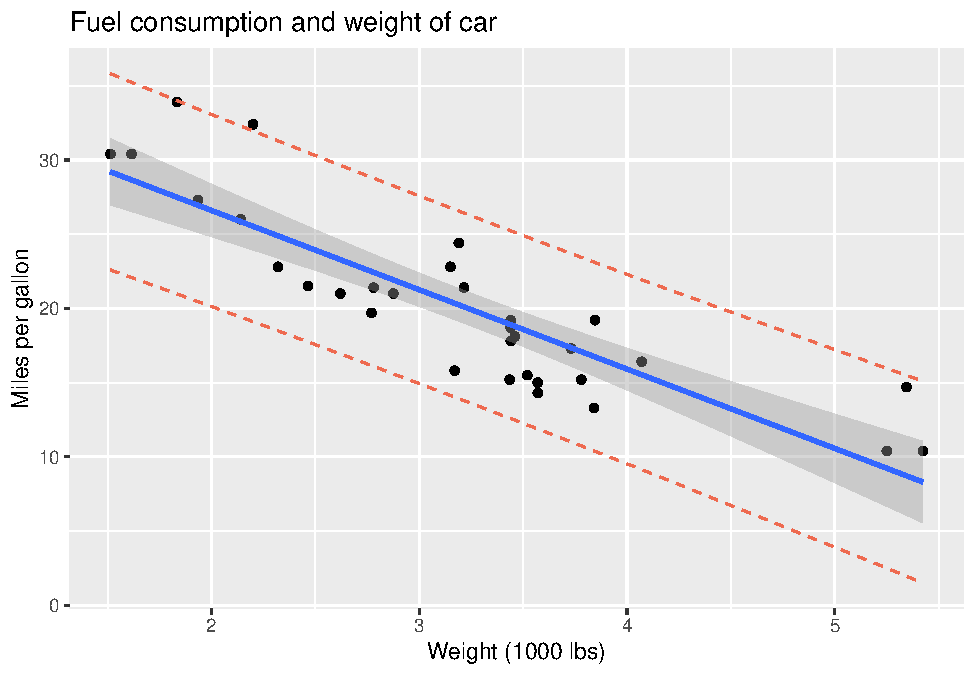
\includegraphics{6G4Z3008-notes_files/figure-latex/predex-1.pdf}
\caption{\label{fig:predex}Confidence intervals appear in grey, and prediction intervals appear in pink.}
\end{figure}

Notice that prediction intervals are generally wider than confidence intervals. We will not derive these formulas, though you are expected to know how to use them, and they appear in the formula book.

Note also that the width of the intervals increases near the ends of the available data, suggesting that there is more uncertainty at the extremes. Notice that the fuel consumption could never go below zero, so extrapolation for this data based on this model would be unreliable for weights above say \(6000\) lbs.

\hypertarget{pmcc}{%
\section{PMCC}\label{pmcc}}

A correlation coefficient is a measure of the strength of the (linear) relationship between two variables.We denote the population correlation coefficient by the Greek letter r - \(\rho\), and the sample correlation coefficient by \(r\).

The Pearson product moment correlation coefficient (PMCC) is closely related to the gradient of a simple linear regression line.

\begin{definition}
Given \(n\) observations \((x_i,y_i)\) where \(1\leq i \leq n\), the ****Pearson product moment correlation coefficient (PMCC)**** is given by

\[r = \frac{s_{xy}}{\sqrt{s_{xx}s_{yy}}}\]
\[=\frac{\sum xy - n\bar{x}\bar{y}}{\sqrt{(\sum x^2 - n\bar{x}^2)(\sum y^2 - n\bar{y}^2)}} \]
\end{definition}

The sign of the correlation is determined by the numerator in this expression. The denominator ensures that the coefficient always lies between the extremes of \(-1\) and \(1\). If the observations lie on a \emph{straight line} then the PMCC equals \(\pm 1\). With real data, it is extremely unlikely due to experimental error.

\begin{example}
The following data shows the age \(x\) (in years) and the second-hand price \(y\) (in hundreds of pounds) of a sample of \(11\) cars advertised online.

\begin{longtable}[]{@{}cccccccccccc@{}}
\toprule
x & 5 & 7 & 6 & 6 & 5 & 4 & 7 & 6 & 5 & 5 & 2\tabularnewline
\midrule
\endhead
y & 80 & 57 & 58 & 55 & 70 & 88 & 43 & 60 & 69 & 63 & 118\tabularnewline
\bottomrule
\end{longtable}

Calculate the PMCC for this data and interpret this in context.

\emph{solution}

One can use the formula or another calculation method, and find that \(r = -0.957\). This indicates a strong negative correlation between the age and the value of a car. In context this means that cars that are less old are worth more than older cars which are worth less (but not worthless).
\end{example}

\hypertarget{pitfalls}{%
\subsection{Pitfalls}\label{pitfalls}}

\begin{itemize}
\item
  Correlation does not imply causation. Even if a causal relationship exists, it may be reverse or due to a third unrelated or unmeasured factor. Ice cream sales and deaths in open water are correlated - why? Tree movement rate and wind speed are causally related, but which is the response? More seriously, this issue appears very often in the media when (mis)reporting findings of medical studies.
\item
  Correlation measures linear relationships. Variables may be perfectly related in a non-linear fashion e.g.~an exponential decay or quadratic curve, but could have zero linear correlation coefficient.
\item
  Correlations may be hidden or exaggerated due to clusters in the data which behave in distinctive ways. A plot of beak length of birds may have different trends for different species.
\item
  The correlation coefficient is not equal to the gradient of the regression line.
\end{itemize}

\hypertarget{hypothesis-tests-for-correlation}{%
\section{Hypothesis tests for correlation}\label{hypothesis-tests-for-correlation}}

It is easy to say if a correlation coefficient is close to \(1\) or \(-1\) that there is a strong correlation - but what if \(r=0.6\)? At what point do we say that there is no correlation, based on this number alone?

The answer is that we can conduct a hypothesis test, using \(r\) as a statistic. We can test the hypotheses:

\[\text{H}_0 : \rho = 0, \ \  \ \  \text{H}_1: \rho \neq 0\]
If the sample correlation coefficient \(r\), in absolute value, exceeds a critical value from tables, then we may reject the null hypothesis.

\begin{example}
The following data refer to the average temperature (in degrees Farenheit) and the average butterfat content for a herd of cows (expressed as a percentage of the milk).

\begin{longtable}[]{@{}ccccccccccc@{}}
\toprule
Temp. & 64 & 65 & 65 & 64 & 61 & 55 & 39 & 41 & 46 & 59\tabularnewline
\midrule
\endhead
Butterfat & 4.65 & 4.58 & 4.67 & 4.6 & 4.83 & 4.55 & 5.14 & 4.71 & 4.69 & 4.65\tabularnewline
\bottomrule
\end{longtable}

\begin{longtable}[]{@{}ccccccccccc@{}}
\toprule
Temp. & 56 & 56 & 62 & 37 & 37 & 45 & 57 & 58 & 60 & 55\tabularnewline
\midrule
\endhead
Butterfat & 4.36 & 4.82 & 4.65 & 4.66 & 4.95 & 4.6 & 4.68 & 4.65 & 4.6 & 4.46\tabularnewline
\bottomrule
\end{longtable}

Test at the \(5\%\) significance level whether there is evidence of any correlation between the two variables.

\emph{solution}

One calculates \(r=-0.453\).

The degrees of freedom equal \(n-2 = 18\).

Comparing this to the tables with level \(5\% /2 = 0.025\) gives \(0.444\).

Therefore as \(|r| = 0.453 > 0.444\) we can reject \(H_0\) and conclude that there is a weakly negative correlation.
\end{example}

Notes.

\begin{itemize}
\item
  Hypothesis testing with the PMCC assumes that the data are a random sample from normal marginals in \(x\) and \(y\). If the data is not a random sample from a normal population, then this analysis is not appropriate.
\item
  In some circumstances wemay wish to test against a one-sided alternative. That is that the correlation is strictly positive or negative. In this situation one should look up the \(5\%\) value rather than the \(2.5\%\) value.
\end{itemize}

\hypertarget{summary-3}{%
\section{Summary}\label{summary-3}}

\begin{itemize}
\tightlist
\item
  A linear model is an equation
\end{itemize}

\[y = a+bx +\varepsilon\]

\begin{itemize}
\tightlist
\item
  There are formulas for \(a\) and \(b\):
  \[a = \bar{y}-b\bar{x},\]
\end{itemize}

\[b = \frac{s_{xy}}{s_{xx}}\]
- Residuals are the difference between the point and the regression line. There are a few useful graphs that can tell if the model is a good fit to the linear model.

\begin{itemize}
\item
  A test for significance for the coefficient \(b\) is done via an ANOVA F-test. The table appears in the formula booklet.
\item
  Confidence and prediction intervals can be calculated to quantify uncertainty about the predicted value of the response.
\item
  Sample correlation can be calculated via
  \[r = \frac{s_{xy}}{\sqrt{s_{xx}s_{yy}}}\]
\item
  There is a hypothesis test to detect if there is a correlation or not.
\end{itemize}

\hypertarget{exercises-week-10}{%
\section{Exercises week 10}\label{exercises-week-10}}

\begin{exercise}

Eight pairs of observations on the variables \(x\) and \(y\) are given below.

\begin{longtable}[]{@{}ccccccccc@{}}
\toprule
x & 1.2 & 0.5 & 0.8 & 0.1 & 2.3 & 1.1 & 1.8 & 2.2\tabularnewline
\midrule
\endhead
y & 8.1 & 4.3 & 7.1 & 3.5 & 12.8 & 8.4 & 9.9 & 11.4\tabularnewline
\bottomrule
\end{longtable}

\begin{enumerate}
\def\labelenumi{\alph{enumi})}
\item
  Calculate \(\sum x\), \(\sum x^2\), \(\sum y\), \(\sum y^2\), \(\sum xy\).
\item
  Find \(\bar{x}\), \(\bar{y}\), \(s_{xx}\), \(s_{yy}\) and \(s_{xy}\)
\item
  Find the values of \(a\) and \(b\) for the regression line \(y=a+bx\).
\end{enumerate}

\end{exercise}

\begin{exercise}

Six pairs of observations on the variables \(x\) and \(y\) are given below.

\begin{longtable}[]{@{}ccccccc@{}}
\toprule
x & 55.7 & 10.4 & 67.1 & 91.2 & 30.8 & 72.1\tabularnewline
\midrule
\endhead
y & 21.2 & 45.9 & 88.3 & 11.4 & 75.4 & 21.4\tabularnewline
\bottomrule
\end{longtable}

\begin{enumerate}
\def\labelenumi{\alph{enumi})}
\item
  Calculate \(\sum x\), \(\sum x^2\), \(\sum y\), \(\sum y^2\), \(\sum xy\).
\item
  Find \(\bar{x}\), \(\bar{y}\).
\item
  Find the values of \(a\) and \(b\) for the regression line \(y=a+bx\).
\end{enumerate}

\end{exercise}

\begin{exercise}

Five pairs of observations on the variables \(x\) and \(y\) are given below.

\begin{longtable}[]{@{}cccccc@{}}
\toprule
y & 357.2 & 284.3 & 435.8 & 571.9 & 101.2\tabularnewline
\midrule
\endhead
x & 0.0149 & 0.0375 & -0.0172 & -0.0345 & 0.0651\tabularnewline
\bottomrule
\end{longtable}

\begin{enumerate}
\def\labelenumi{\alph{enumi})}
\item
  Calculate \(\sum x\), \(\sum x^2\), \(\sum y\), \(\sum y^2\), \(\sum xy\).
\item
  Find \(\bar{x}\), \(\bar{y}\).
\item
  Find the values of \(a\) and \(b\) for the regression line \(y=a+bx\).
\item
  Estimate the value of \(y\) when \(x=0.0572\).
\end{enumerate}

\end{exercise}

\begin{exercise}

When a car isdriven under specified conditionsofload, tyre pressure and surrounding temperature, the temperature \(T^{o}C\), generated in the shoulder of the tyre varieswith the speed \(V \ \text{km}/\text{h}\), according to a linear model \(T=a+bV\). Measurements of \(T\) were made at eight different values of \(V\) with the following results.

\begin{longtable}[]{@{}ccccccccc@{}}
\toprule
v & 20 & 30 & 40 & 50 & 60 & 70 & 80 & 90\tabularnewline
\midrule
\endhead
t & 45 & 52 & 64 & 66 & 91 & 86 & 98 & 104\tabularnewline
\bottomrule
\end{longtable}

Given the following

\[\sum v = 440, \ \sum v^2 = 28400, \ \sum t =606, \ \sum t^2 = 49278, \ \sum vt = 37000 \]

\begin{enumerate}
\def\labelenumi{\alph{enumi})}
\item
  Calculate the estimated regression line of \(T\) on \(V\).
\item
  Estimate the value of \(T\) when \(V=60\).
\item
  Calculate the ANOVA table for the data.
\item
  Test the hypothesis \(\text{H}_0: b=0\).
\end{enumerate}

\end{exercise}

\begin{exercise}

An anemometer is used to estimate wind speed by observing the rotational speed of its vanes. This speed is converted to wind speed by means of an equation obtained from calibrating the instrument in a wind tunnel. In this calibration the wind speed is fixed precisely and the resulting anemometer seed is noted. For a particular anemometer this process produced the following set of data.

\begin{longtable}[]{@{}cc@{}}
\toprule
Actual speed (m/s) & Anemometer revs (rev/min)\tabularnewline
\midrule
\endhead
1.0 & 30\tabularnewline
1.1 & 38\tabularnewline
1.2 & 48\tabularnewline
1.3 & 58\tabularnewline
1.4 & 68\tabularnewline
1.5 & 80\tabularnewline
1.6 & 92\tabularnewline
1.7 & 106\tabularnewline
1.8 & 120\tabularnewline
1.9 & 134\tabularnewline
\bottomrule
\end{longtable}

\begin{enumerate}
\def\labelenumi{\alph{enumi})}
\item
  Obtain the least squares regression line for these data
\item
  Calculate an ANOVA table for these data
\item
  Test the hypothesis \(\text{H}_0: b=0\).
\item
  Calculate a \(95\%\) prediction interval for when the actual wind speed is \(1.65 m/s\)
\item
  Give an example using a relevant calculation with the regression line, that it is unwise to extrapolate outside the range of this data.
\end{enumerate}

\end{exercise}

\begin{exercise}

A hospital doctor was interested in the percentage of a certain drug absorbed by patients. She obtained the following data on \(10\) patients taking the drug on two separate days.

\begin{longtable}[]{@{}ccc@{}}
\toprule
Patient & Day 1, x & Day 2, y\tabularnewline
\midrule
\endhead
1 & 35.5 & 27.6\tabularnewline
2 & 16.6 & 15.1\tabularnewline
3 & 13.6 & 12.9\tabularnewline
4 & 42.5 & 34.1\tabularnewline
5 & 28.5 & 35.5\tabularnewline
6 & 30.3 & 32.5\tabularnewline
7 & 8.7 & 84.3\tabularnewline
8 & 21.5 & 21.5\tabularnewline
9 & 16.4 & 11.1\tabularnewline
10 & 32.3 & 36.4\tabularnewline
\bottomrule
\end{longtable}

\begin{enumerate}
\def\labelenumi{\alph{enumi})}
\item
  Calculate the product moment correlation coefficient \(r\) for this data.
\item
  Test at the \(5\%\) significance level whether or not there is no correlation. That is \(H_0:\rho = 0\).
\item
  After examining a plot of the data, the doctor found one of the points was surprising. This result was an anomaly and excluded from the analysis. The \(r\) value for the remaining \(9\) points is \(0.863\). Which point was omitted?
\end{enumerate}

\end{exercise}

  \bibliography{book.bib,packages.bib}

\end{document}
